\documentclass[11pt,oneside,a4paper,english,french,spanish,brazil]{abntex2}

% ----------------------------------------------------------------------------------------
% - Librerias
  \usepackage{sty/modal_configs}    
  \usepackage{sty/datos_portada}      
  \usepackage{sty/modal_dados}              
   \usepackage{sty/modal_vocabulario}         
  \usepackage{sty/modal_leiaute_rt} 
  
  \definecolor{mycolor}{RGB}{0.122, 0.435, 0.698}% Rule colour
  
\captionsetup[figure]{labelformat=empty}% redefines the caption setup of the figures environment in the beamer class.


% ----------------------------------------------------------------------------------------
% - INICIO
  \begin{document}
%      \begin{sloppypar}

          % Seleciona o idioma do documento (conforme pacotes do babel)
            \selectlanguage{spanish}

          % Retira espaço extra obsoleto entre as frases.
            \frenchspacing

          % ------------------------------------------------------------------------------
          % - ESTRUTURA DO DOCUMENTO
          % ------------------------------------------------------------------------------
          % ------------------------------------------------------------------------------
          % - PRÉ-TEXTUAL
          % ------------------------------------------------------------------------------
          \pagestyle{modalpre}

          % Portada
            %~~~~~~~~~~~~~~~~~~~~~~~~~~~~~~~~~~~~~~~~~~~~~~~~~~~~~~~~~~~~~~~~~~~~~
% File  : capa
%~~~~~~~~~~~~~~~~~~~~~~~~~~~~~~~~~~~~~~~~~~~~~~~~~~~~~~~~~~~~~~~~~~~~~

% Limpa os estilos de página
  \thispagestyle{empty}

% Desenho no fundo da página
  \ThisCenterWallPaper{1}{sty/pulso_portada.pdf}

% Cria uma mini-página para inserir os dados da capa usando 70% da largura do texto
    \begin{minipage}{0.85\textwidth}
    \end{minipage}%

    \vspace{14cm}
    \begin{minipage}{0.85\textwidth}
      \begin{center}
          % Rodapé da capa
          \sffamily
          
          \rule{\textwidth}{0.2mm}
          \textbf{\ppidata} \\[0.5cm]
          \textbf{Versión Preliminar} \\[0.5cm]
%          Orientador: \textbf{\Orientador} \\[-0.2cm]
          \rule{\textwidth}{0.2mm}\\
      \end{center}
    \end{minipage}%
    


            \clearpage

          % Metadata
            %~~~~~~~~~~~~~~~~~~~~~~~~~~~~~~~~~~~~~~~~~~~~~~~~~~~~~~~~~~~~~~~~~~~~~
% File  : revisoes
%~~~~~~~~~~~~~~~~~~~~~~~~~~~~~~~~~~~~~~~~~~~~~~~~~~~~~~~~~~~~~~~~~~~~~

% Tabela de revisões do plano de trabalho

    %\ABNTEXchapterfont
    \setlength{\parindent}{0cm}

    \vspace*{\fill}

    {\sffamily \Large Autores}

        \begin{tabular}{r p{12cm}}
            \hline
            \emph{Equipo BID:}     & Priscilla Grissel Gutierrez Juarez\\
            \emph{Equipo Universidad EAFIT} & 	Mónica Hernandez y Juan Carlos Muñoz  \\
            \emph{Investigadores Junior:}  & Germán Angulo y Ana Pirela\\
            \emph{Versión:}      & \ppiversao \\
            \hline
        \end{tabular}

%----------------------------------------------------------------------

            \clearpage

          % Sumarios
            \vspace{1cm}
            \tableofcontents
            \clearpage
            
            \vspace{1cm}
            \listoffigures
            \clearpage

            \vspace{1cm}
            \listoftables

            \clearpage
  
          % ------------------------------------------------------------------------------
          % - Introducción
          % -----------------------------------------------------------------------------
          %~~~~~~~~~~~~~~~~~~~~~~~~~~~~~~~~~~~~~~~~~~~~~~~~~~~~~~~~~~~~~~~~~~~~~
% File  : capa
%~~~~~~~~~~~~~~~~~~~~~~~~~~~~~~~~~~~~~~~~~~~~~~~~~~~~~~~~~~~~~~~~~~~~~

% Limpa os estilos de página
  \thispagestyle{empty}

% Desenho no fundo da página
  \ThisCenterWallPaper{1}{sty/pulso_titulos.pdf}

% Cria uma mini-página para inserir os dados da capa usando 70% da largura do texto
    \begin{minipage}{0.85\textwidth}
    \end{minipage}%

    \vspace{14cm}
    \begin{minipage}{0.85\textwidth}
      \begin{center}
          % Rodapé da capa
          \sffamily
          
          \rule{\textwidth}{0.2mm}
          \chapter{Introducción}
%          Orientador: \textbf{\Orientador} \\[-0.2cm]
          \rule{\textwidth}{0.2mm}\\
      \end{center}
    \end{minipage}%
    


          \clearpage
          \newpage
          
          \pagestyle{modal}
          

    %%% Introducción Pulso Social
    El presente informe
    
    
    %%% Los principales 
    
    \begin{tcolorbox}[enhanced,fit to height=10cm, colback=mycolor,colframe=mycolor,drop fuzzy shadow,watermark color=white,
                        %%% Title
                        title=Principales Resultados]
    \begin{itemize}
        \item Las brechas de ingreso por género son muy grandes, especialmente en los percentiles más bajos de ingreso.
        \item El ingreso de las mujeres está rezagado 10 años con respecto al de los hombres, en los percentiles más bajos.
        \item La tasa de mujeres jóvenes que ni estudian, ni trabajan es casi el doble que la de los hombres jóvenes. Esta brecha se agudizó con la pandemia.
         \item Gran brecha de ingreso entre minorías y no minorías  en todos los niveles de ingreso.
        \item A pesar de que la pobreza ha disminuido, las diferencias entre regiones todavía son muy altas.
        \item La pandemia del COVID-19 causó un aumento preocupante en las tasas de pobreza en las zonas urbanas, al punto de hacerla converger con la de las zonas  rurales.
     \end{itemize}
    \end{tcolorbox}




           \clearpage
        % ------------------------------------------------------------------------------
          % - Contexto
          % -----------------------------------------------------------------------------
          %~~~~~~~~~~~~~~~~~~~~~~~~~~~~~~~~~~~~~~~~~~~~~~~~~~~~~~~~~~~~~~~~~~~~~
% File  : capa
%~~~~~~~~~~~~~~~~~~~~~~~~~~~~~~~~~~~~~~~~~~~~~~~~~~~~~~~~~~~~~~~~~~~~~

% Limpa os estilos de página
  \thispagestyle{empty}

% Desenho no fundo da página
  \ThisCenterWallPaper{1}{sty/pulso_titulos.pdf}

% Cria uma mini-página para inserir os dados da capa usando 70% da largura do texto
    \begin{minipage}{0.85\textwidth}
    \end{minipage}%

    \vspace{14cm}
    \begin{minipage}{0.85\textwidth}
      \begin{center}
          % Rodapé da capa
          \sffamily
          
          \rule{\textwidth}{0.2mm}
          \chapter{Indicadores de Contexto}
%          Orientador: \textbf{\Orientador} \\[-0.2cm]
          \rule{\textwidth}{0.2mm}\\
      \end{center}
    \end{minipage}%
    


          \clearpage
          \newpage
          
          \pagestyle{modal}
 
           


\section{Ingreso Familiar}

    %%%%---------------------
    %%% Principales resultados
    %%%%---------------------
    \begin{tcolorbox}[enhanced, colback=mycolor,colframe=mycolor,drop fuzzy shadow,watermark color=white,
                        %%% Título
                        title=Principales Resultados]
    

                    \begin{itemize}
                    \item Pero hay una brecha de género enorme, especialmente en los percentiles más bajos de ingreso.
                    \item El rezago en el ingreso de las mujeres con respecto al de los hombres es de más de 10 años.
                \end{itemize}
     
     
    \end{tcolorbox}
    %%%%---------------------
    %%%%---------------------
    %%%%---------------------



    \subsection{Ingreso Laboral}
 %%%% Include figures
    \begin{figure}[H]
    \caption[Percentil 25 del ingreso laboral por ciudades principales - 2019]{\label{ingreso_laboral_25_ciudades}}
        \begin{center}
        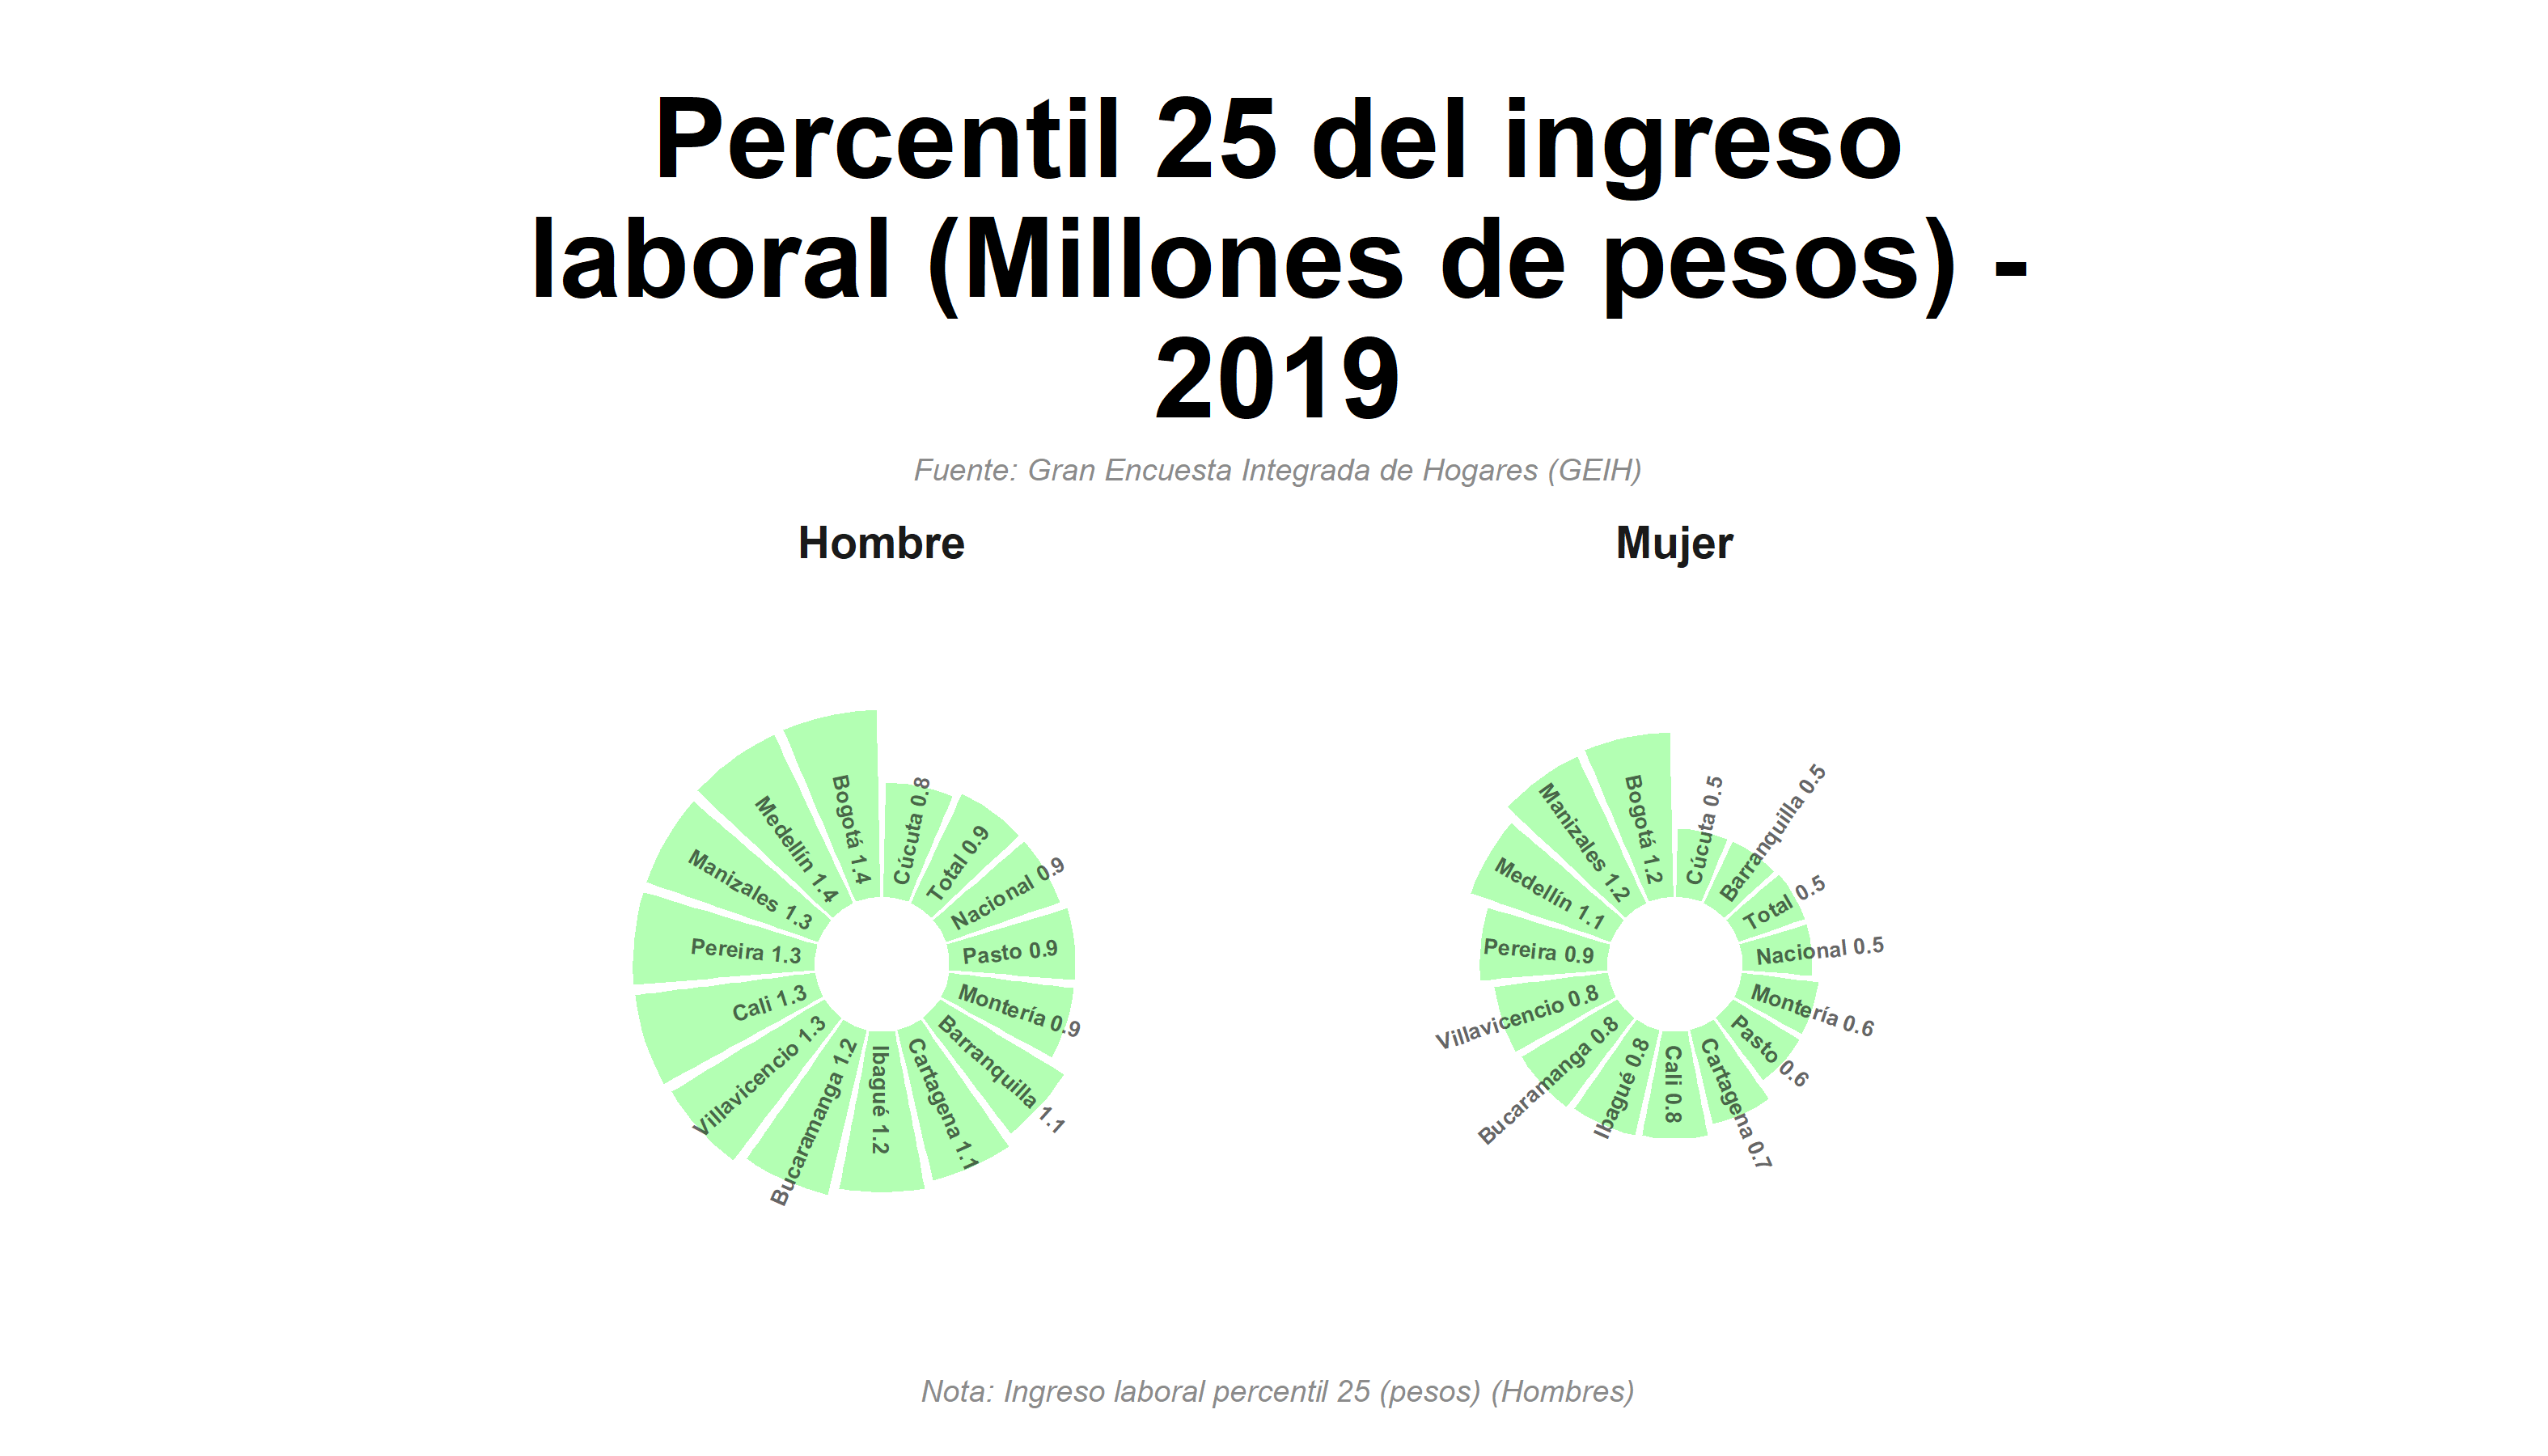
\includegraphics[width=\textwidth,keepaspectratio]{img/var_2_static.png}
        \end{center}
    \end{figure}
            \begin{itemize}
                    \item Hay una diferencia de ingreso de más de un millón entre la ciudad de menor ingreso y la de mayor (Cúcuta -  Bogotá).
                    \item Todas las ciudades principales están por encima del promedio nacional a excepción de Cúcuta.
                \end{itemize}

 %%%% Include figures
    \begin{figure}[H]
        \caption[Percentil 25 del ingreso laboral por ciudades principales para minorías - 2020]{\label{ingreso_laboral_25_ciudades_minorias} }
        \begin{center}
        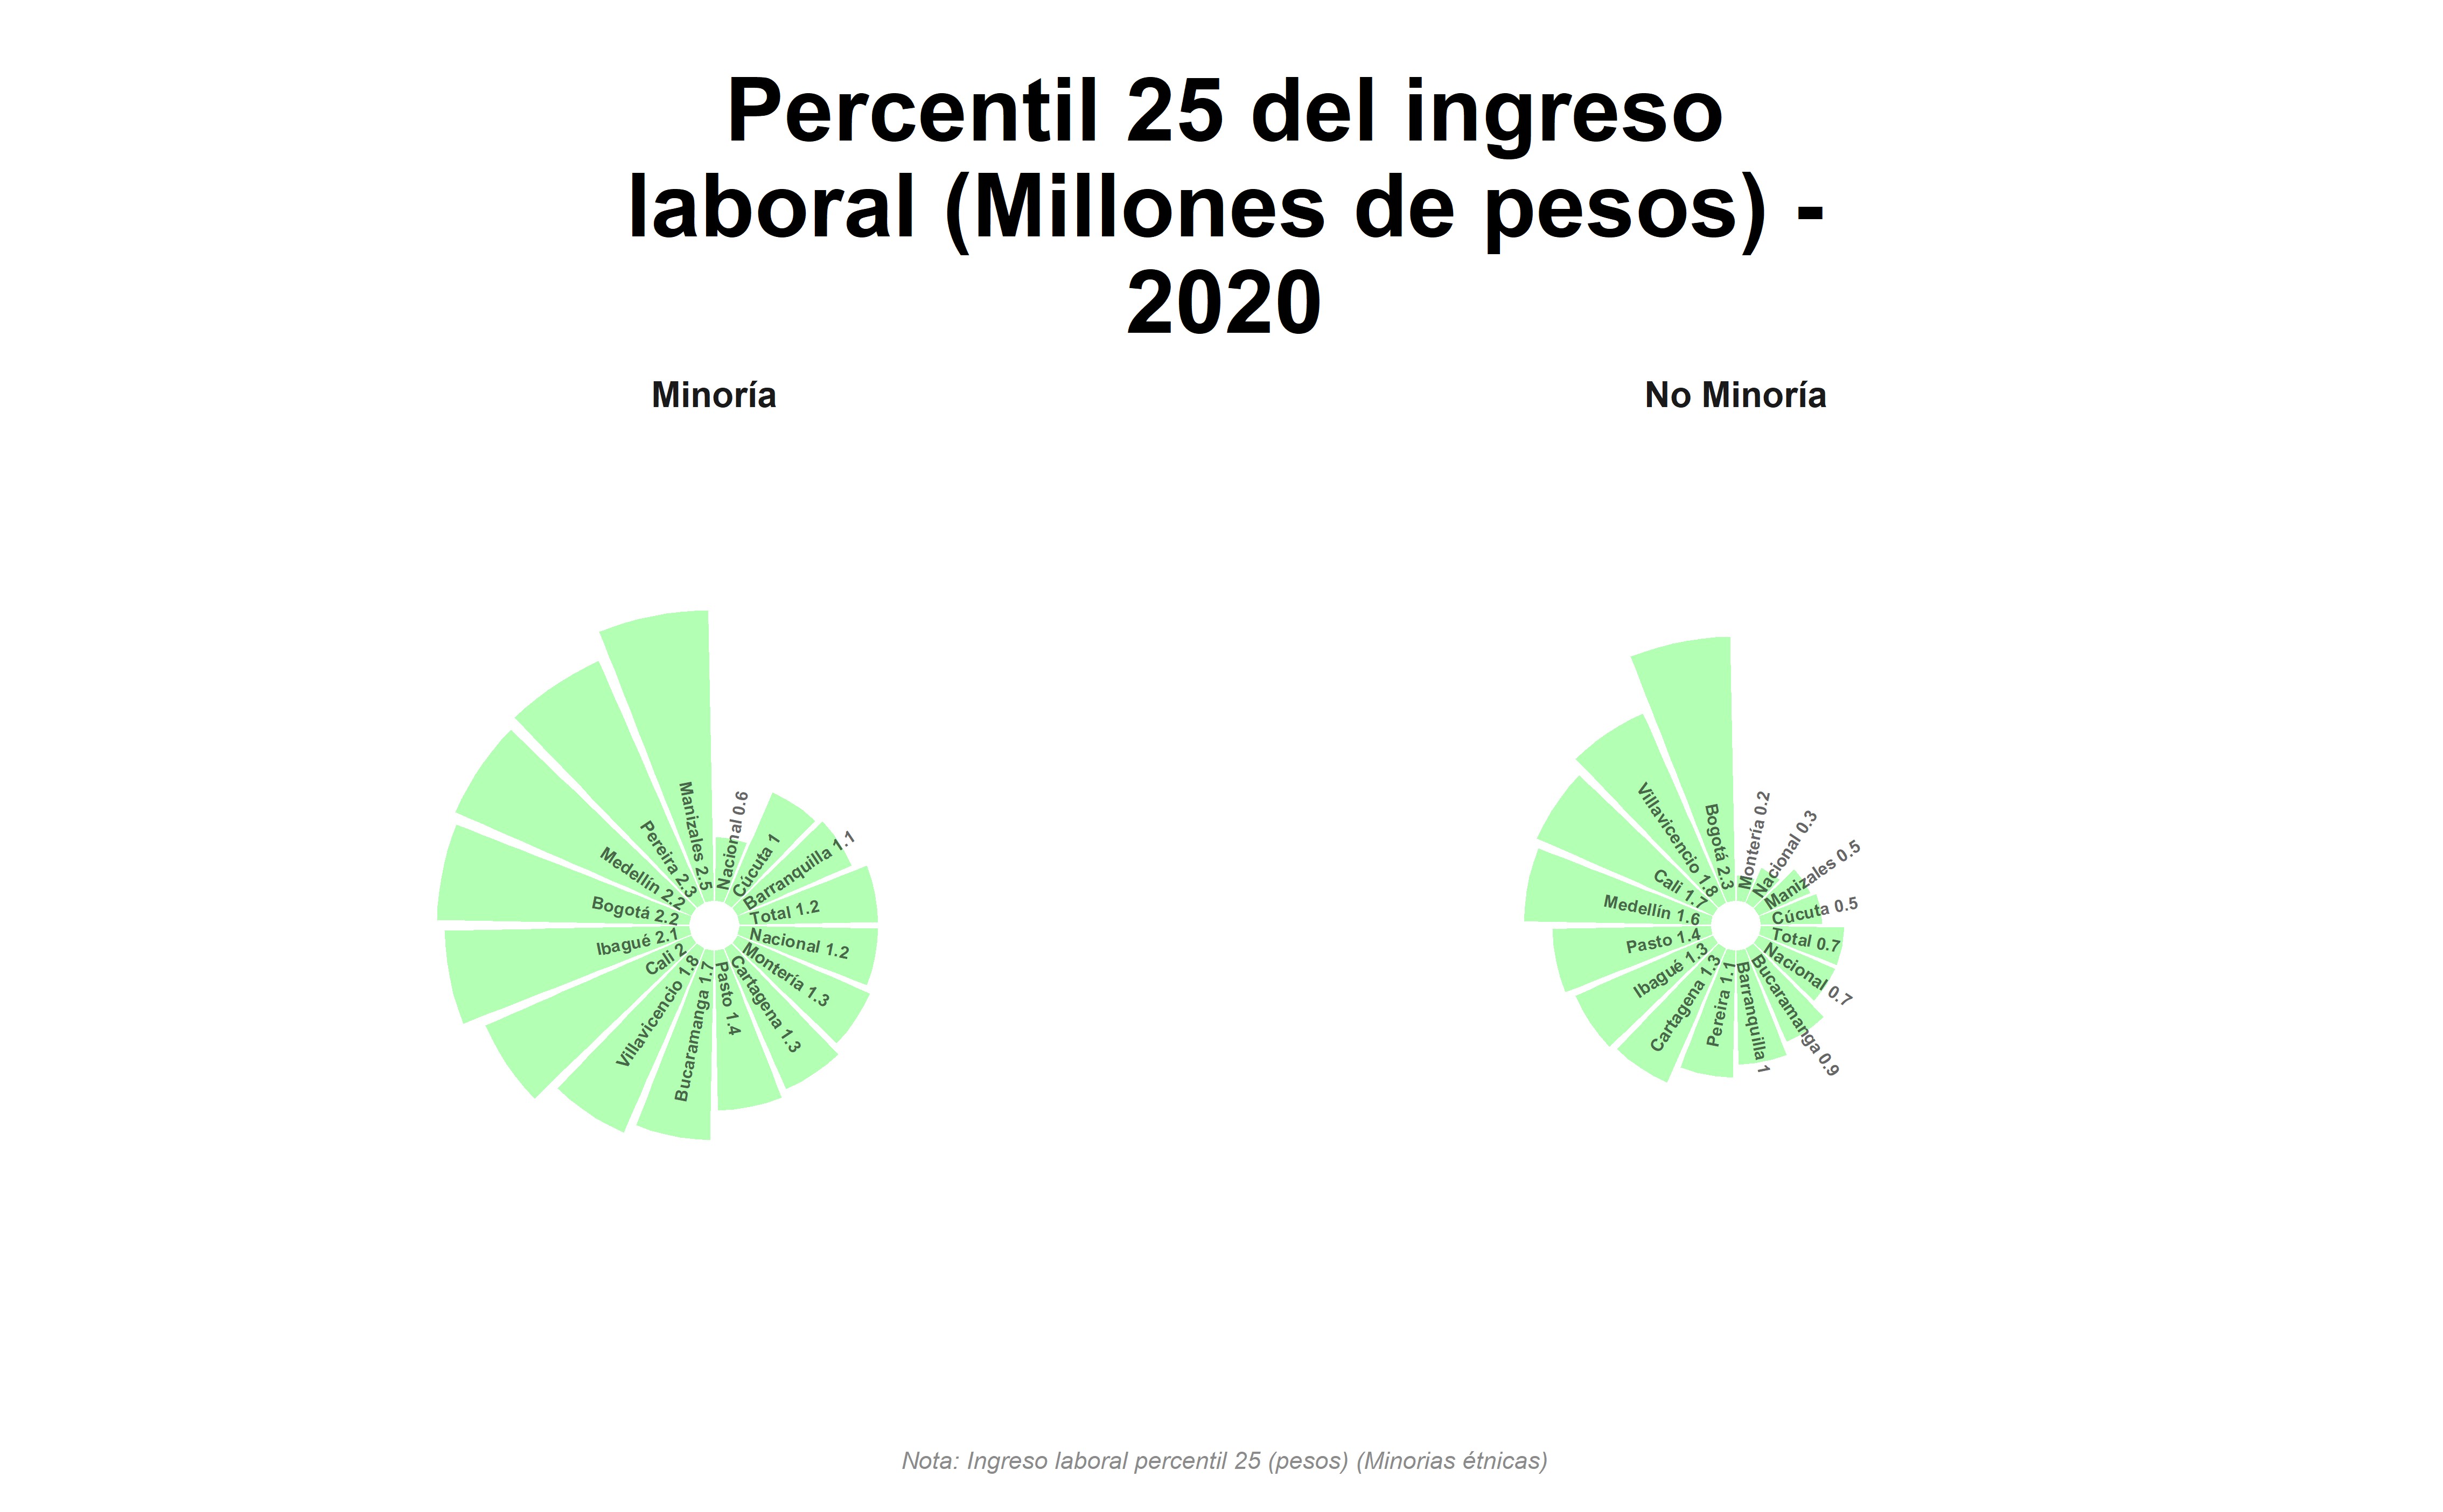
\includegraphics[width=\textwidth,keepaspectratio]{img/var_1_static.png}
        \end{center}
    \end{figure}
            \begin{itemize}
                    \item Hay una diferencia de ingreso de alrededor de 2 millones entre la ciudad de mayor ingreso y la de menor para minorías (Cúcuta -  Manizales) y no minorías (Montería - Bogotá).
                    \item Todas las ciudades principales están por encima del promedio nacional a excepción de Montería en el caso de las no minorías.
                    \item En general las minorías tienen ingresos mayores con respecto a las no minorías en el percentil más bajo de ingresos.
                \end{itemize}

%%%% Include figures
    \begin{figure}[H]
        \caption[Percentil 25 del ingreso laboral por ciudades principales - 2010 VS 2019 ]{\label{ingreso_laboral_25_ciudades_VS} }
        \begin{center}
        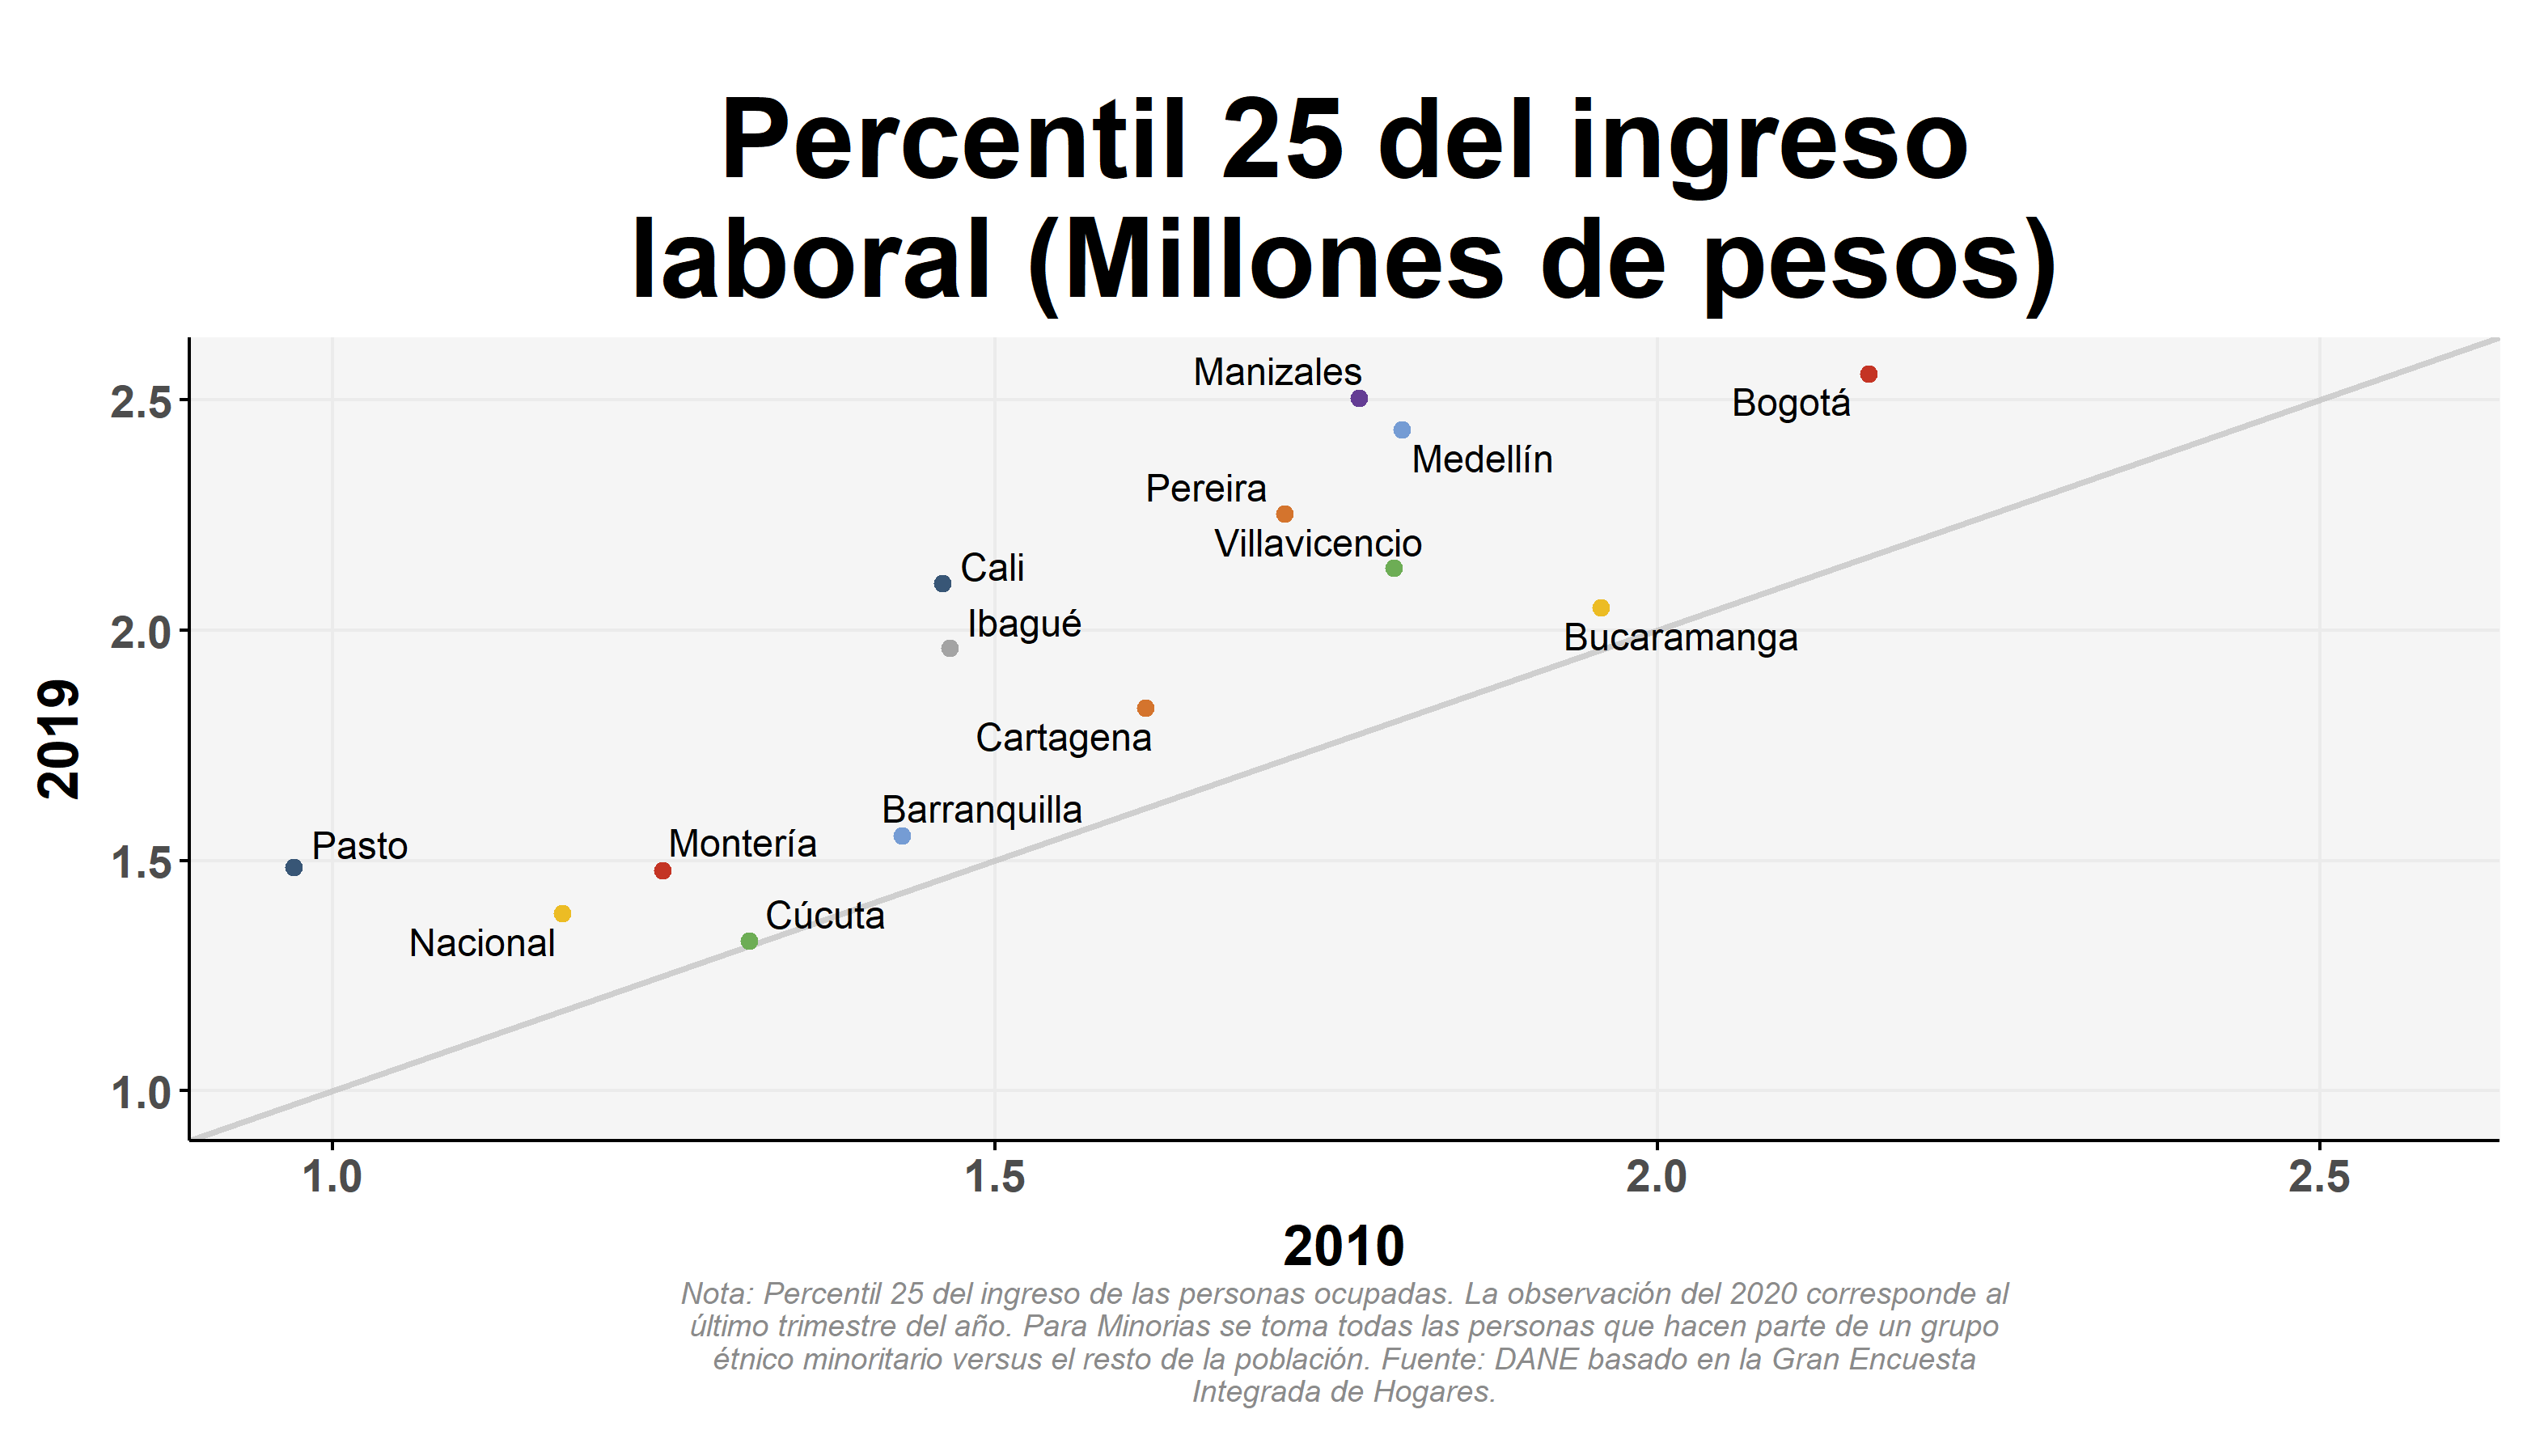
\includegraphics[width=\textwidth,keepaspectratio]{img/var_2_scatter_time.png}
        \end{center}
    \end{figure}
            \begin{itemize}
                    \item Todas las ciudades mejoraron en los últimos 10 años el ingreso laboral en el percentil a excepción de Cúcuta que se mantiene igual.
                    \item Ciudades que hace 10 años tenían similares ingresos pero unas mejoraron más significativamente que otras, caso Ibagué y Cali, y Villavicencio y Medellín.
                \end{itemize}

%%%% Include figures
    \begin{figure}[H]
        \caption[Percentil 25 del ingreso laboral por género]{ \label{ingreso_laboral_25_genero} }
        \begin{center}
        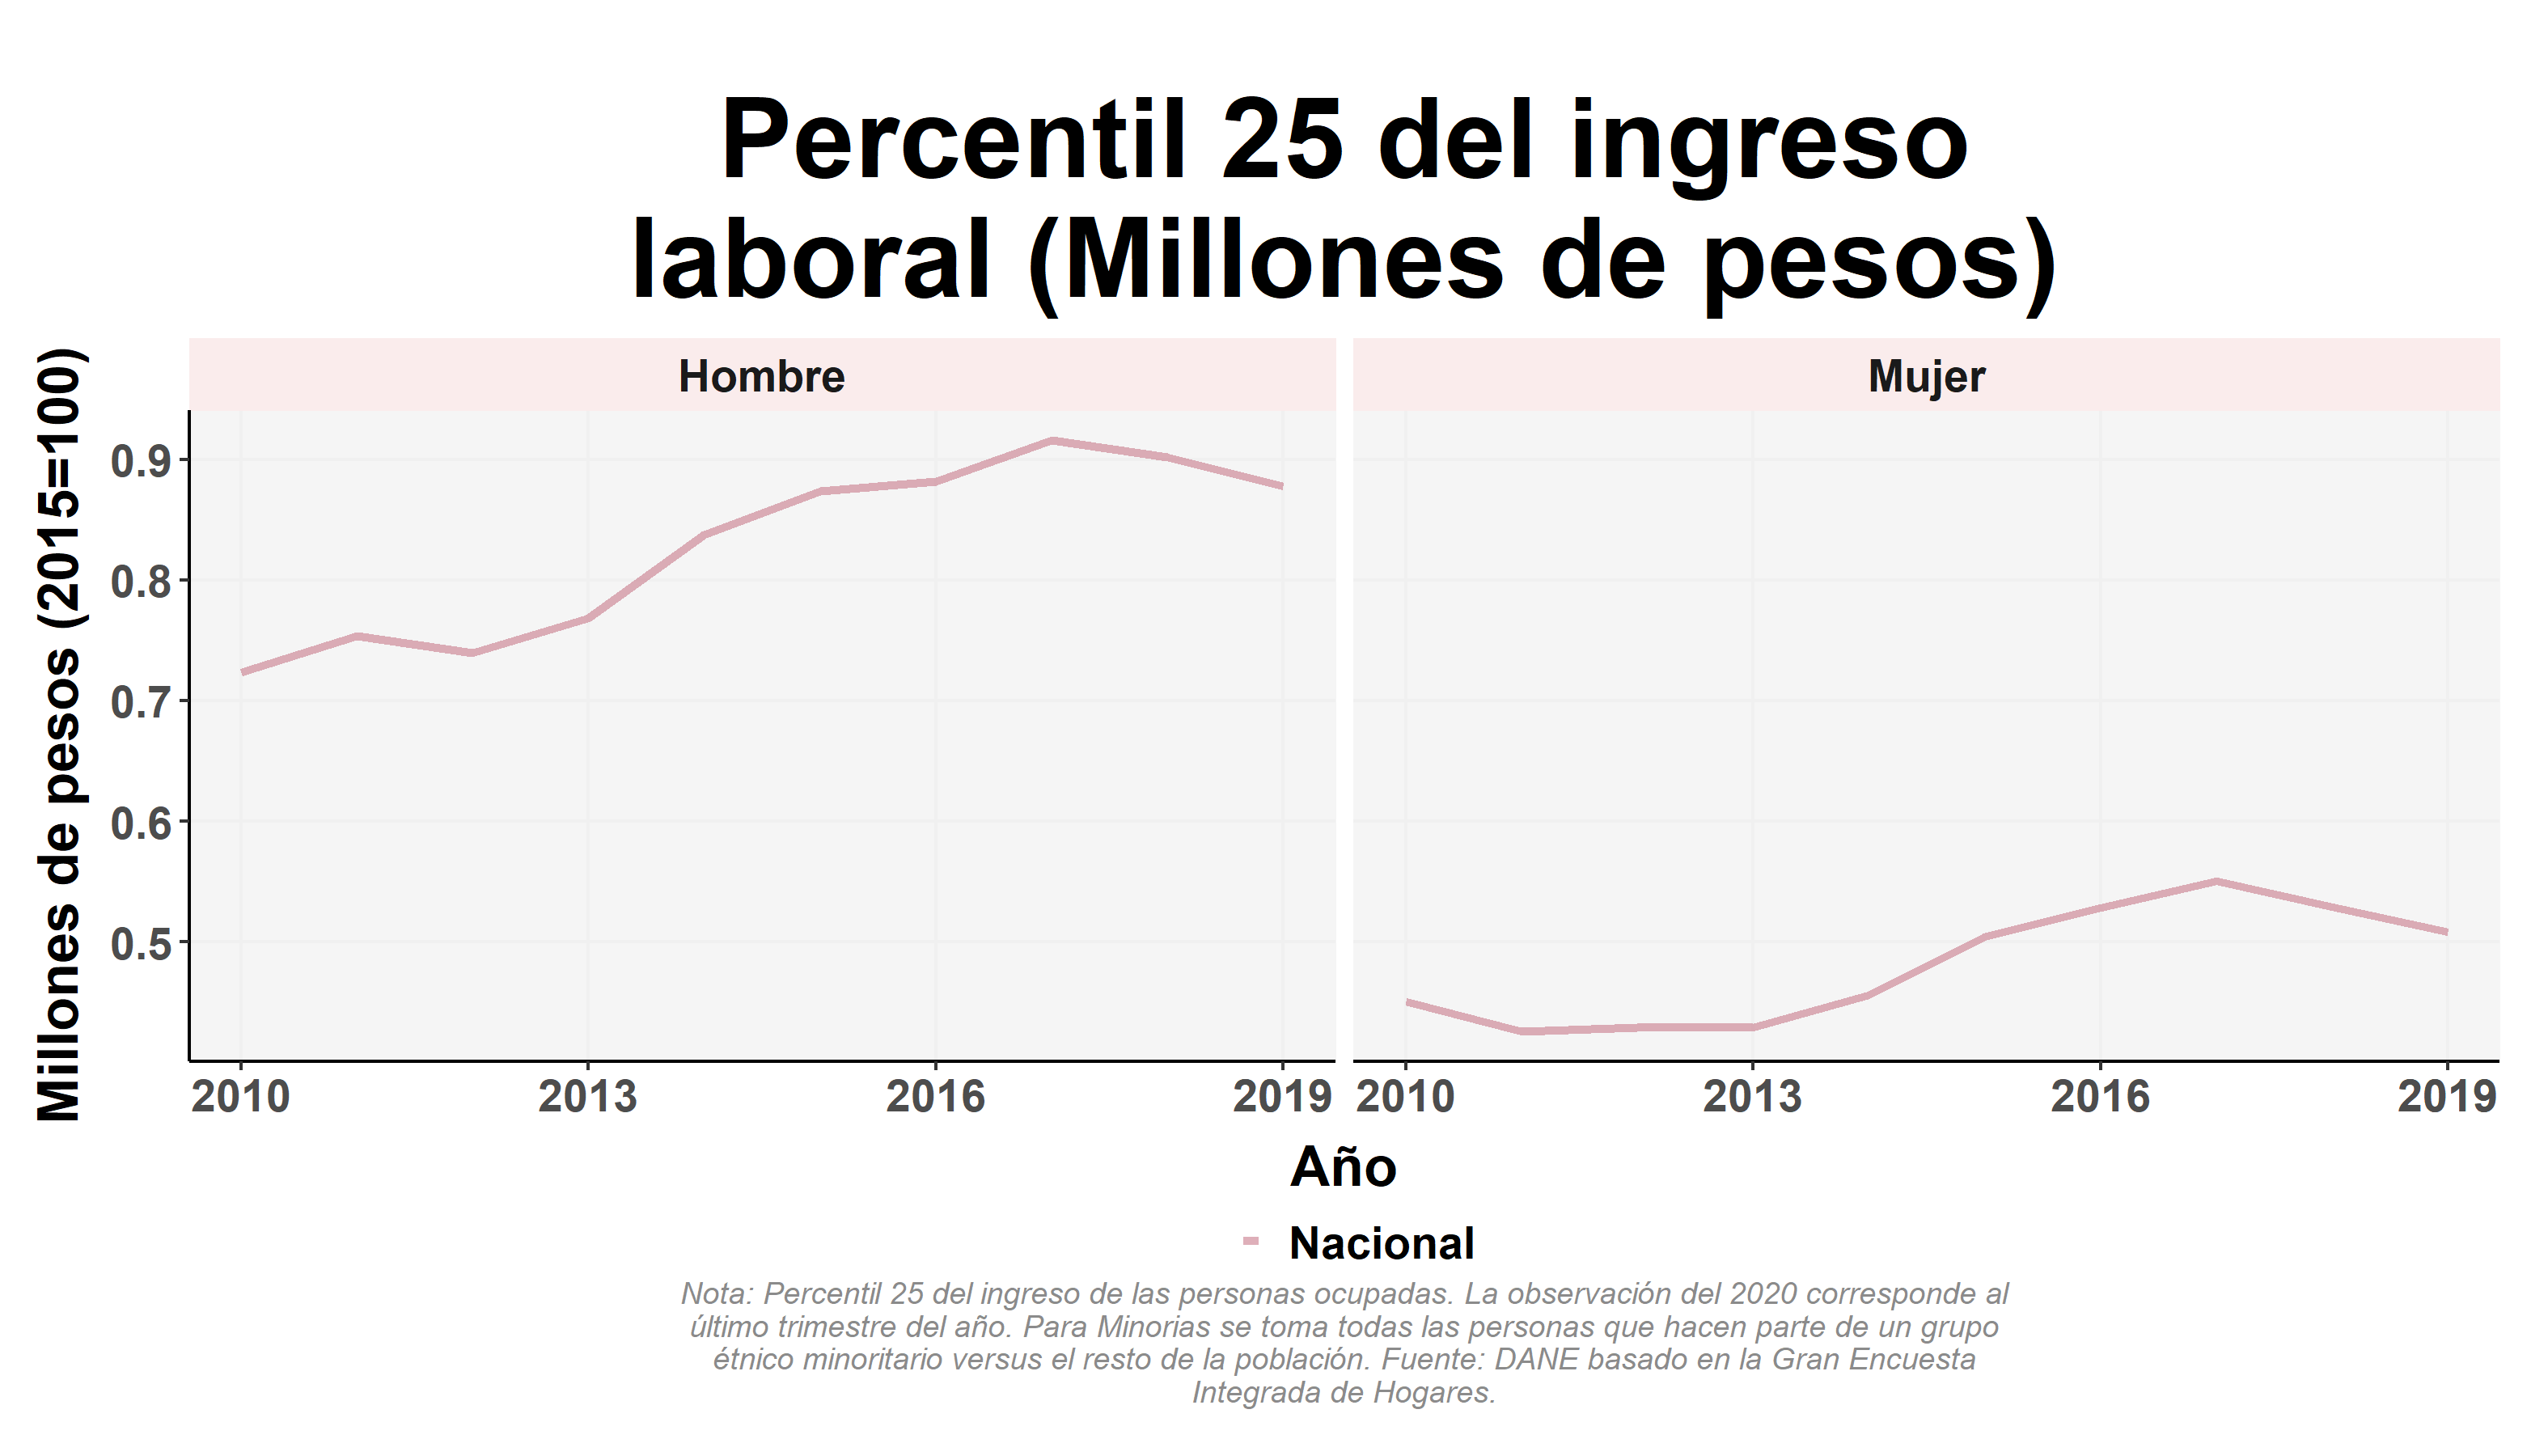
\includegraphics[width=\textwidth,keepaspectratio]{img/var_4_trend.png}
        \end{center}
    \end{figure}
            \begin{itemize}
                    \item Brecha enorme en el ingreso por género en el percentil más bajo, una mujer en el 2019 gana mucho menos que un hombre lo hacía en el 2010.
                    \item Los ingresos estaban aumentando hasta el 2017, pero el del hombre lo hacia de manera más contante que el de la mujer.
                    \item El ingreso venía disminuyendo desde el 2018, y se incentiva más en el 2020 con el Covid. Esto también de ve en el ámbito nacional.
                \end{itemize}

 %%%% Include figures
    \begin{figure}[H]
    \caption[Percentil 50 del ingreso laboral por ciudades principales - 2019]{\label{ingreso_laboral_50_ciudades}}
        \begin{center}
        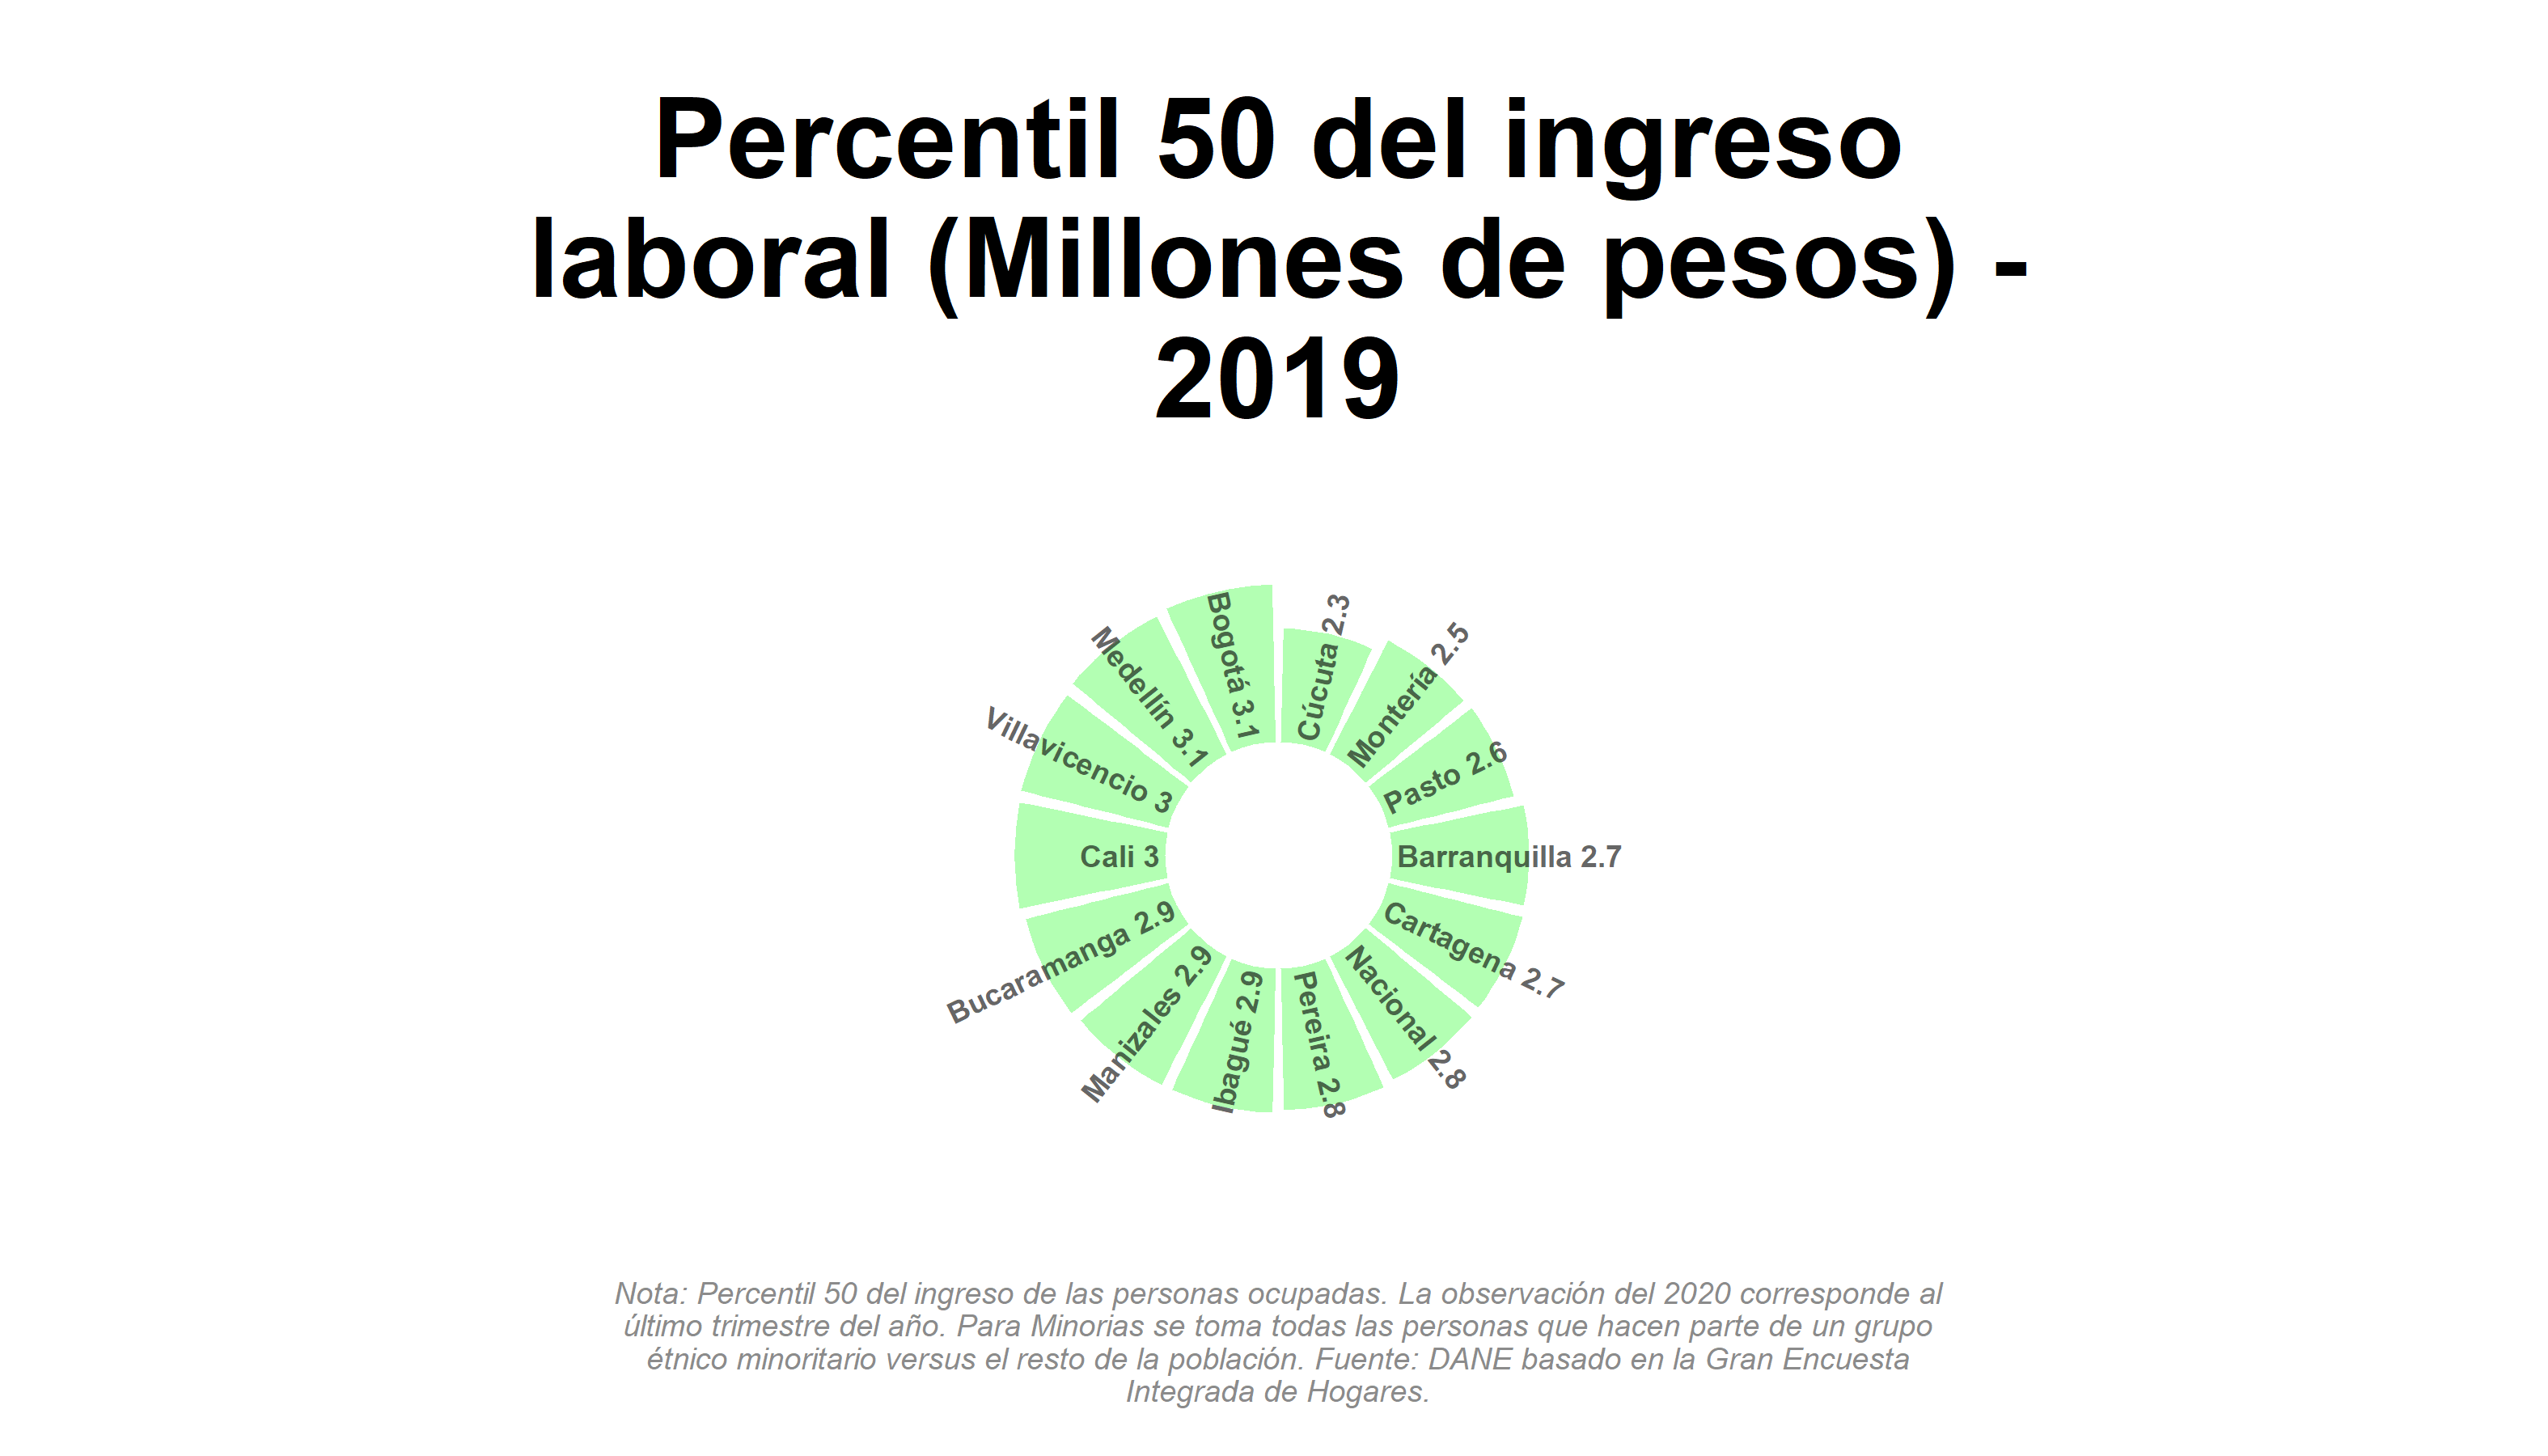
\includegraphics[width=\textwidth,keepaspectratio]{img/var_25605_static.png}
        \end{center}
    \end{figure}
            \begin{itemize}
                    \item El ingreso laboral para el percentil 50 está por encima de los 2 millones en las principales ciudades.
                    \item Entre la ciudad de mayor y menor ingreso laboral en el percentil 50 hay una diferencia de 800 mil pesos aproximadamente (Bogotá - Cúcuta).
                \end{itemize}

%%%% Include figures
    \begin{figure}[H]
        \caption[Percentil 50 del ingreso laboral por ciudades principales para minorías - 2020]{ \label{ingreso_laboral_50_ciudades_minoria} }
        \begin{center}
        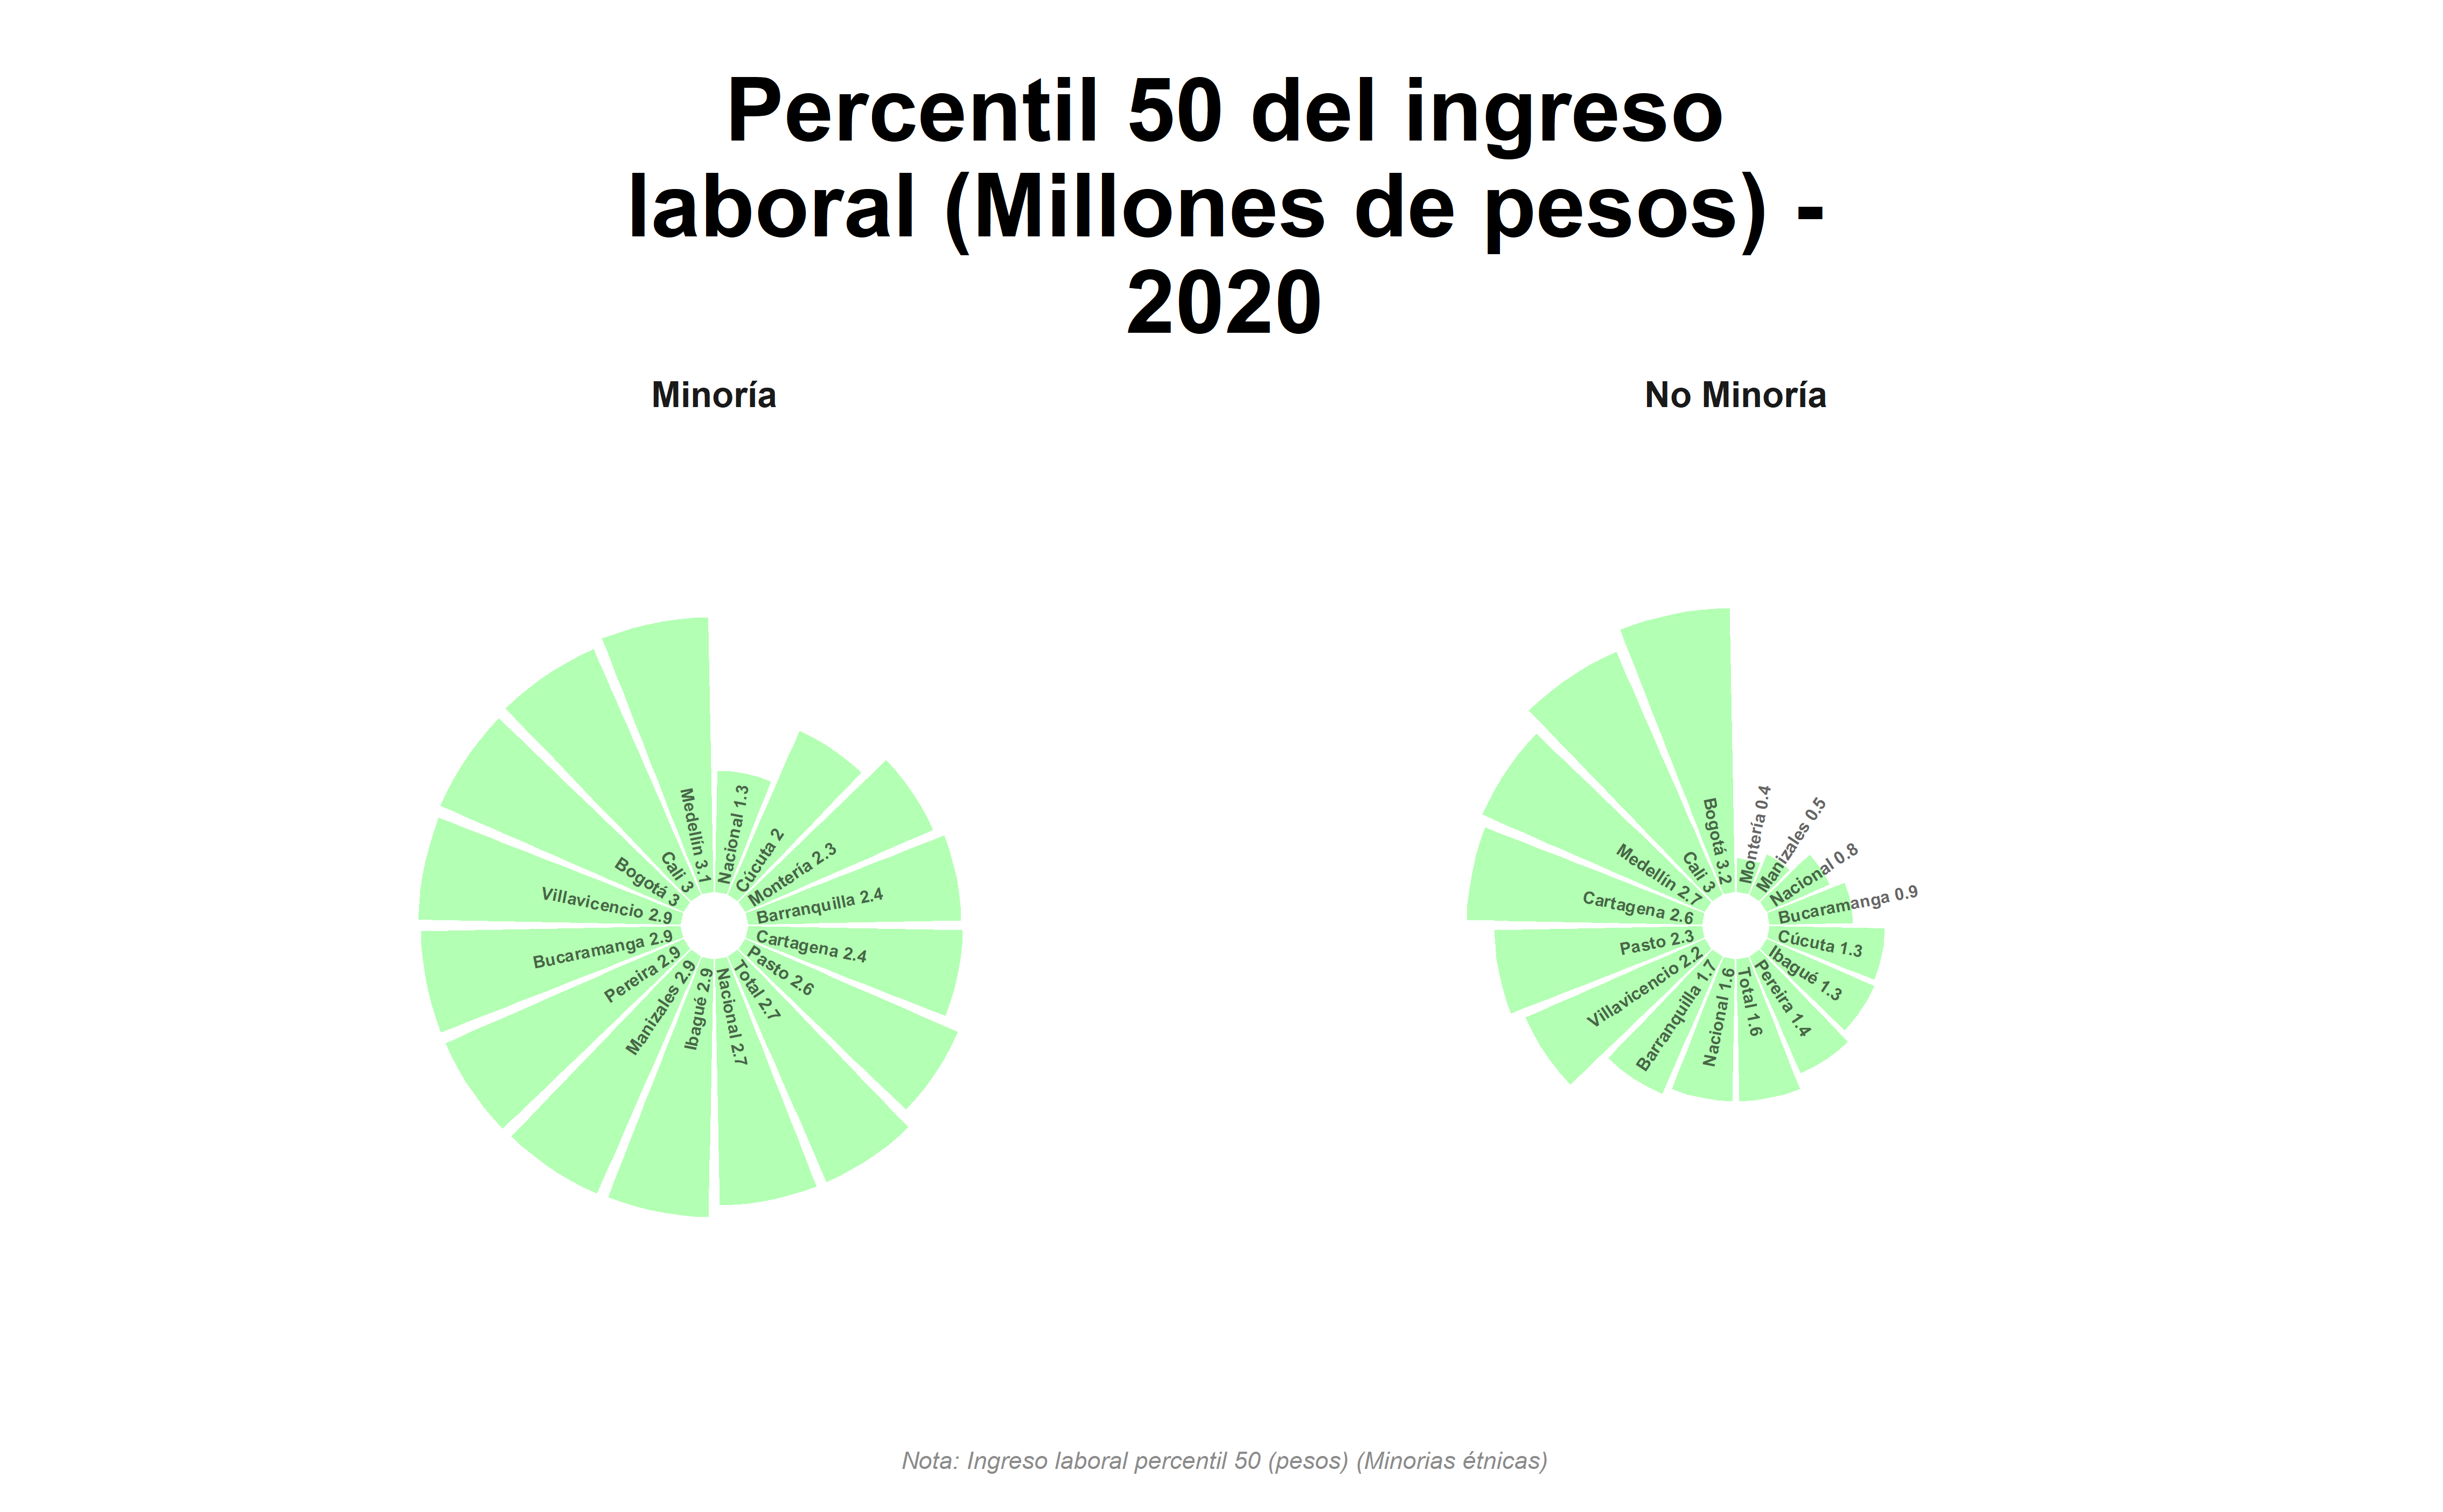
\includegraphics[width=\textwidth,keepaspectratio]{img/var_14_static.png}
        \end{center}
    \end{figure}
            \begin{itemize}
                    \item Diferencia en el ingreso medio de poco más de un millón entre ciudades para minorías (Cúcuta - Medellín), y cerca de tres millones para las no minorías (Montería - Bogotá).
                    \item El ingreso medio nacional es mayor para las no minorías, mismo comportamiento con  Bogotá y Cartagena, mientras que las otras sigue siendo mayor en las minorías.
                    \item El ingreso medio en el caso de las minorías se ve más equitativo que el de las no minorías.
                \end{itemize}

 %%%% Include figures
    \begin{figure}[H]
    \caption[Percentil 50 del ingreso laboral por ciudades principales - 2010 VS 2019]{\label{ingreso_laboral_50_ciudades_vs}}
        \begin{center}
        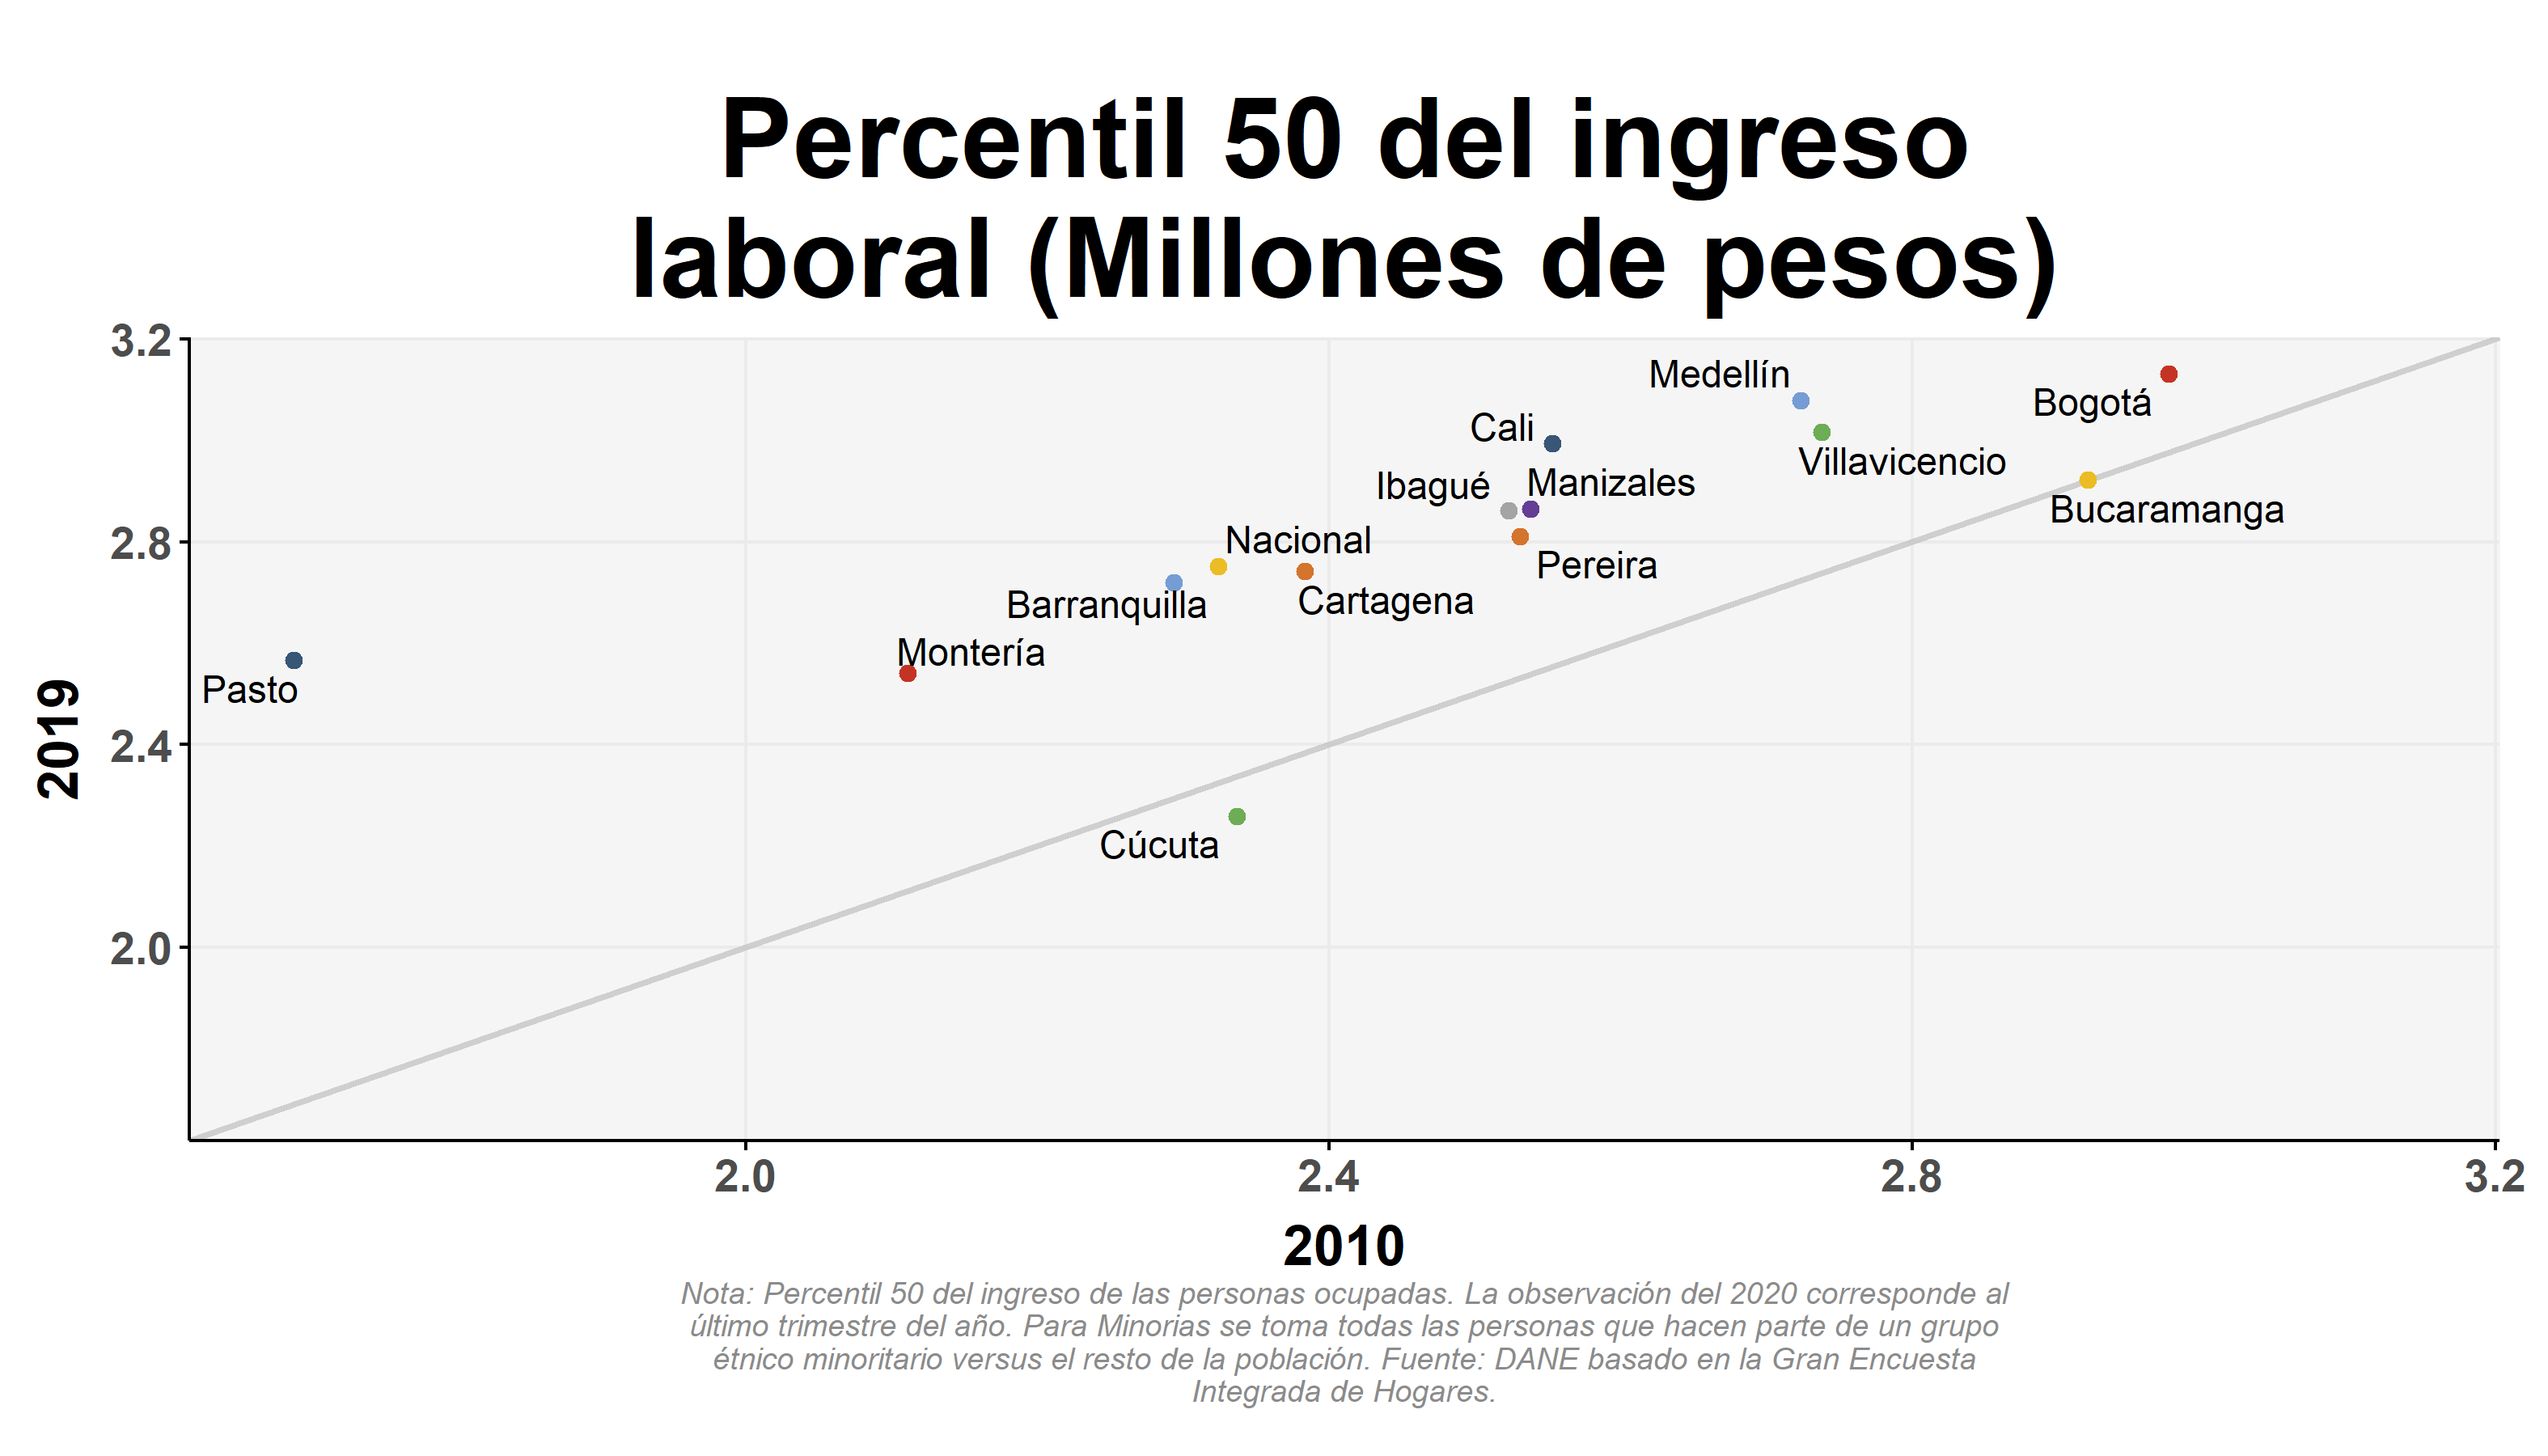
\includegraphics[width=\textwidth,keepaspectratio]{img/var_25605_scatter_time.png}
        \end{center}
    \end{figure}
            \begin{itemize}
                    \item Cúcuta es la única ciudad que presentó un menor ingreso laboral en el percentil 50 para 2020 comparado con el 2010.
                    \item Bucaramanga se mantiene con el mismo nivel de ingreso laboral entre 2010 y 2020.
                    \item Aunque las demás ciudades presentan mejoras, se destaca que Pasto pasó de ser una de las ciudades con menor ingreso laboral, por debajo de 2 millones, a tener poco más de 2.5 millones en promedio para 2020.
                \end{itemize}

%%%% Include figures
    \begin{figure}[H]
        \caption[Percentil 50 del ingreso laboral por género]{ \label{ingreso_laboral_50_genero} }
        \begin{center}
        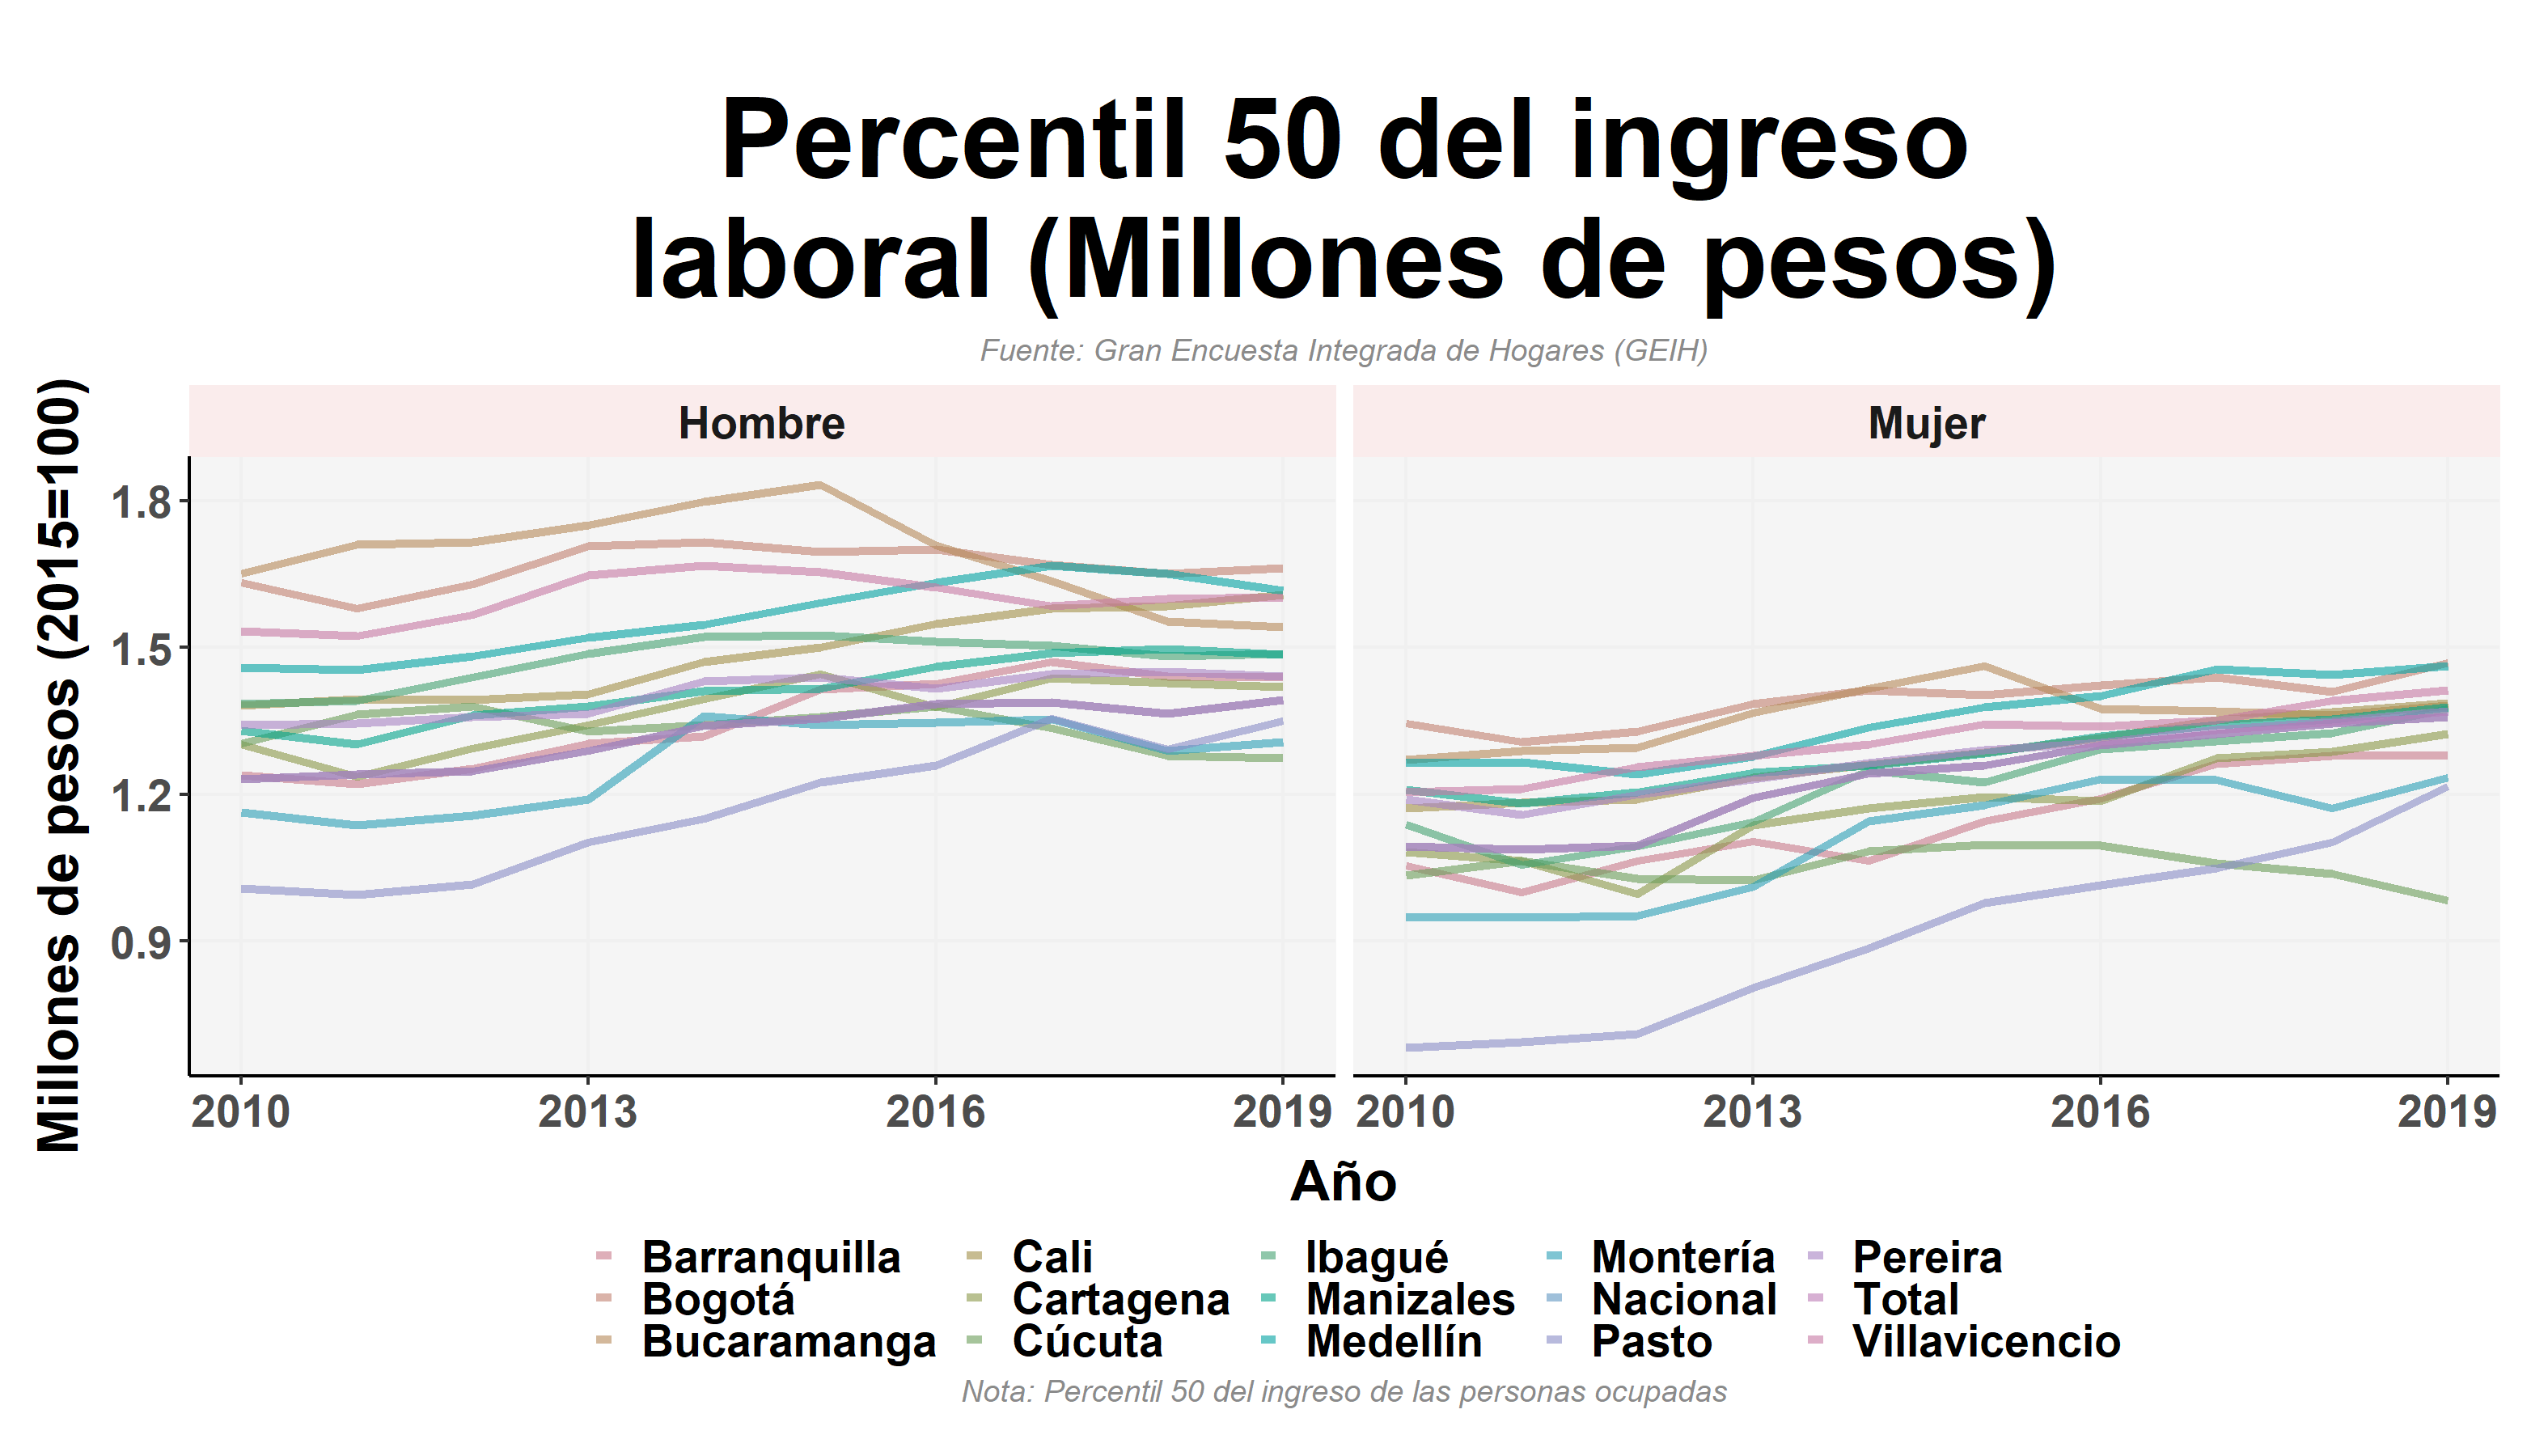
\includegraphics[width=\textwidth,keepaspectratio]{img/var_16_trend.png}
        \end{center}
    \end{figure}
            \begin{itemize}
                    \item El ingreso por género en el percentil 50 tiene menos diferencia a comparación como en el percentil 25.
                    \item La diferencia entre géneros muestra que hace 10 años era más de cien mil y ahora es menor.
                    \item El ingreso de la mujer ha aumentado de manera constante desde el 2012, mientras que el del hombre se ha mantenido igual desde el 2016, con una caída en el 2018.
                    \item Los ingresos por género en el percentil 50 han mejorado con el tiempo, de igual manera se ve que lo ha hecho el total nacional.
                \end{itemize}

%%%% Include figures
    \begin{figure}[H]
        \caption[Percentil 75 del ingreso laboral por ciudades principales para 2019]{\label{ingreso_laboral_75_ciudades} }
        \begin{center}
        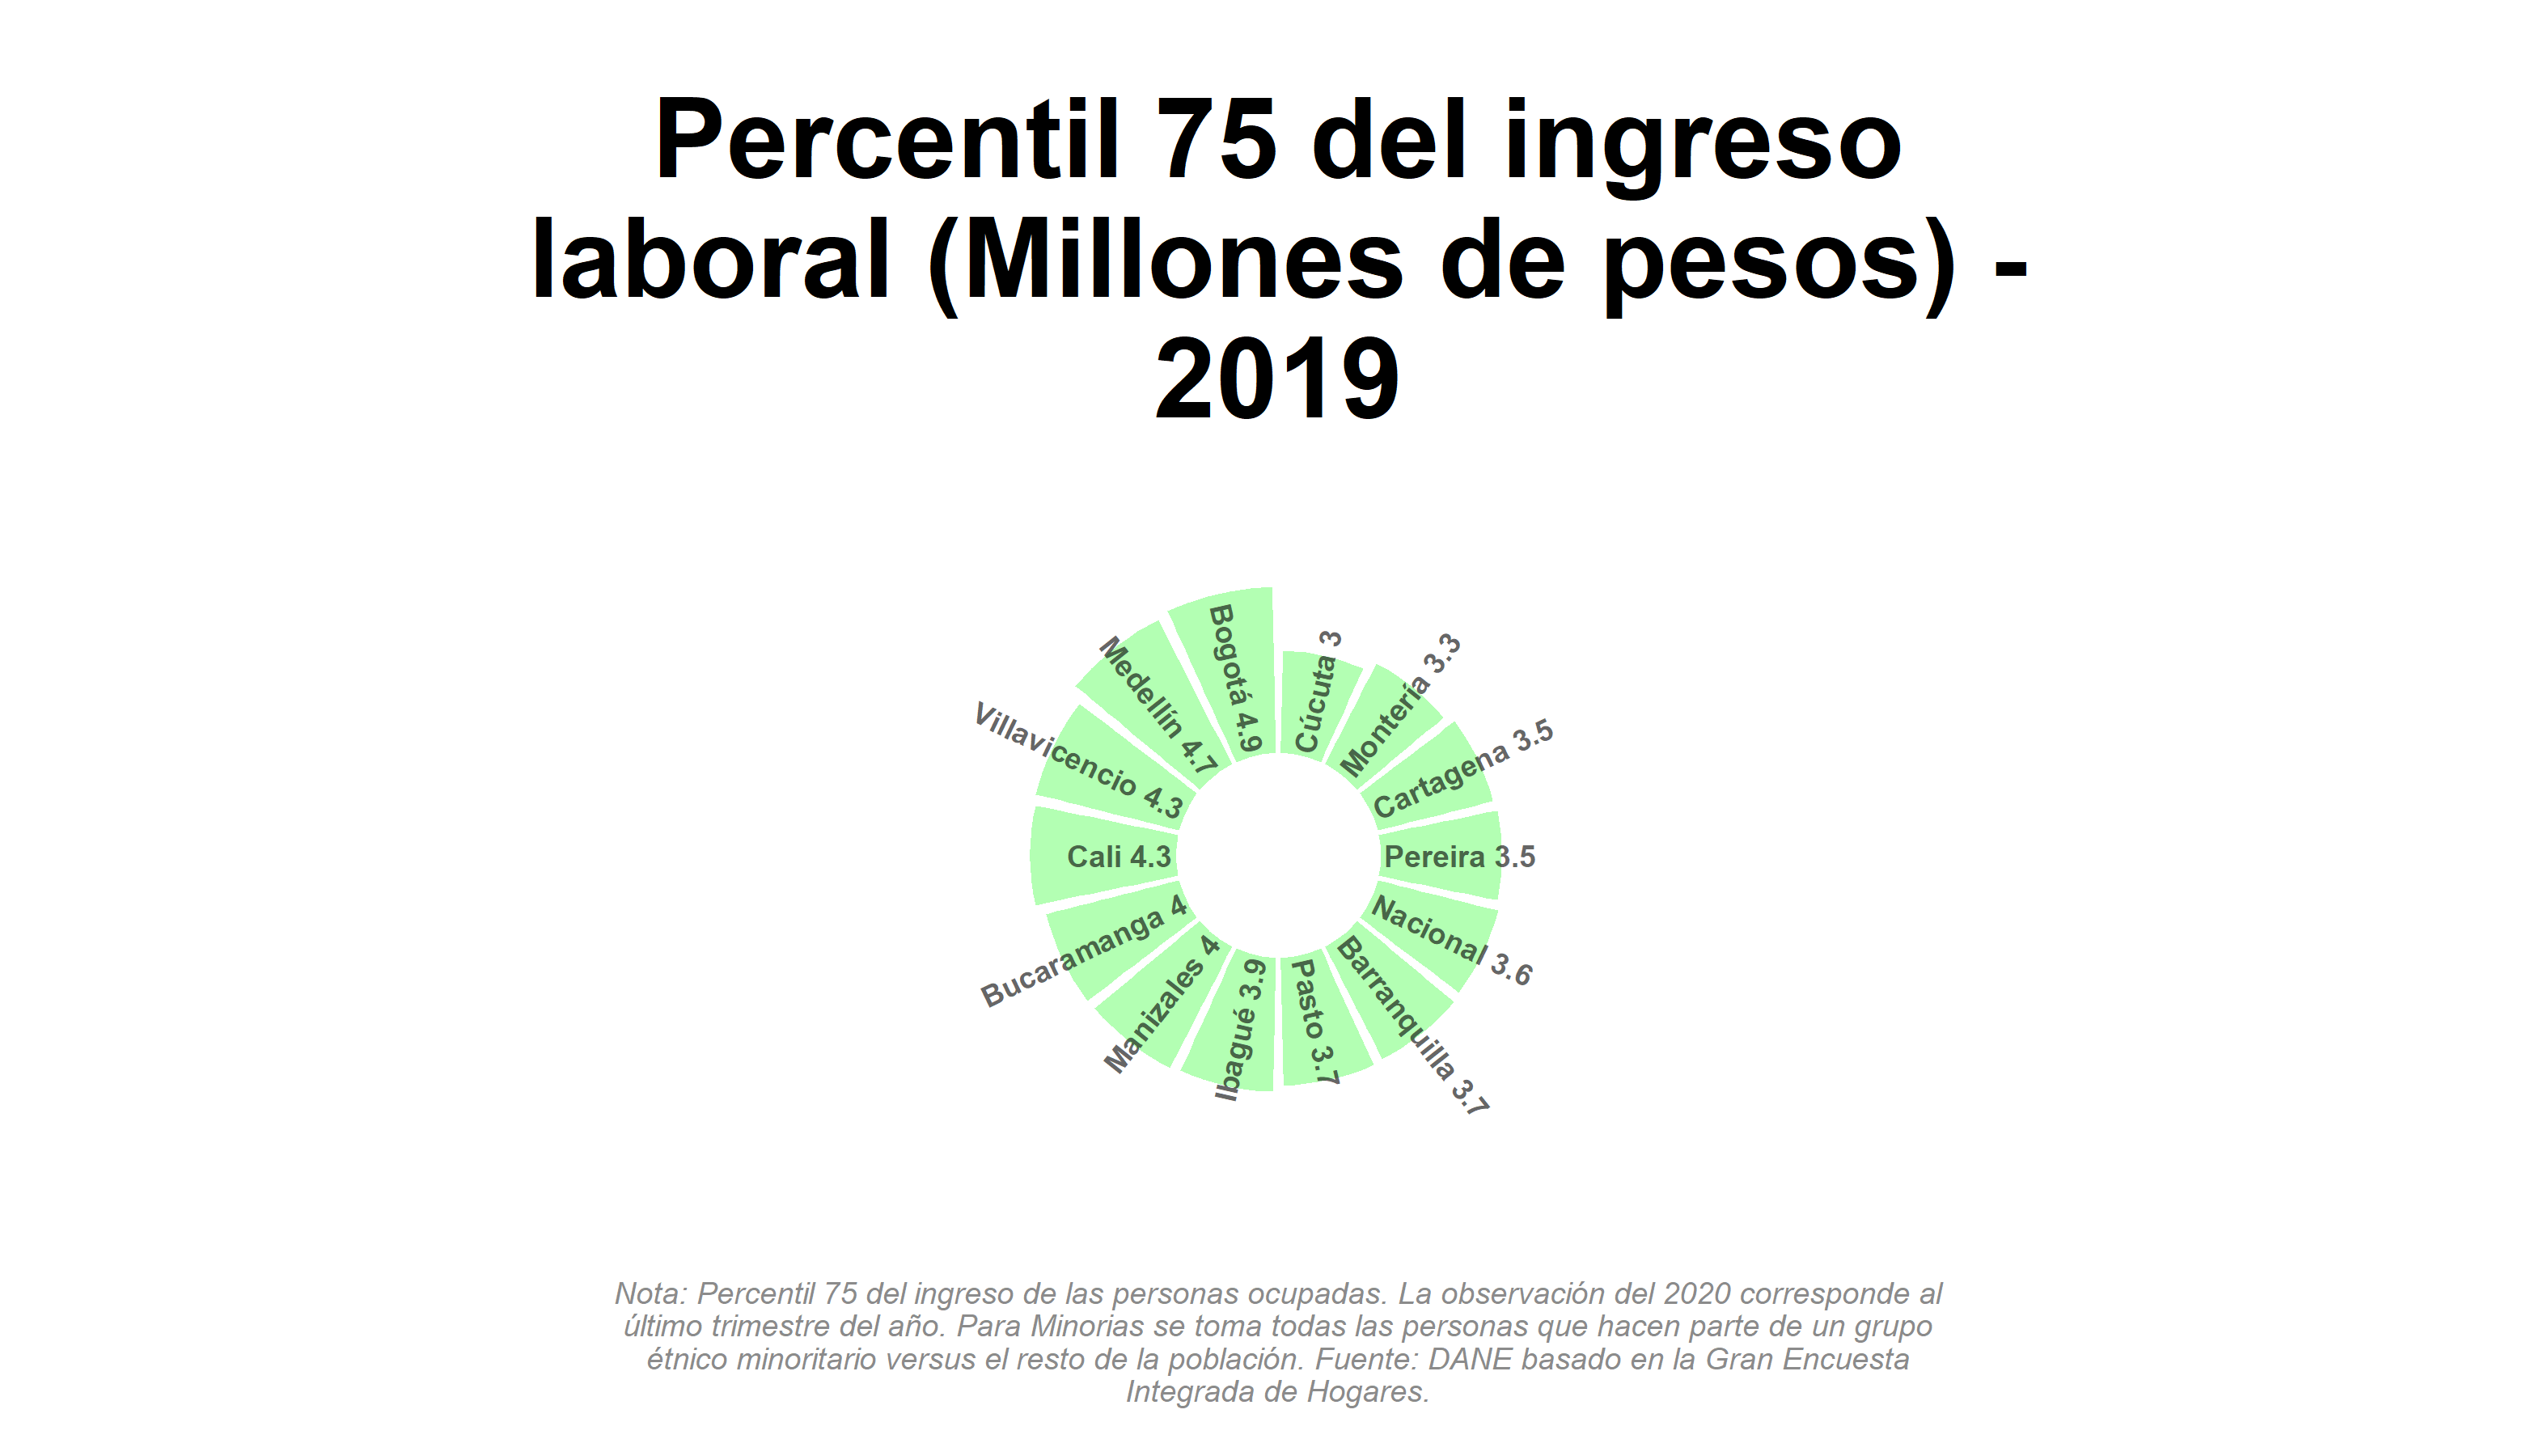
\includegraphics[width=\textwidth,keepaspectratio]{img/var_26455_static.png}
        \end{center}
    \end{figure}
            \begin{itemize}
                    \item En las ciudades principales el ingreso laboral es mínimo 3 millones.
                    \item Hay una diferencia de casi 2 millones entre la ciudad con mayor ingreso, Bogotá, y la de menor, Cúcuta.
                    \item Cúcuta, Montería, Cartagena y Pereira son las únicas ciudades cuyo ingreso laboral en el percentil 75 es menor al promedio nacional.
                \end{itemize}

%%%% Include figures
    \begin{figure}[H]
        \caption[Percentil 75 del ingreso laboral por ciudades principales para minorías - 2020]{\label{ingreso_laboral_75_ciudades_minorias} }
        \begin{center}
        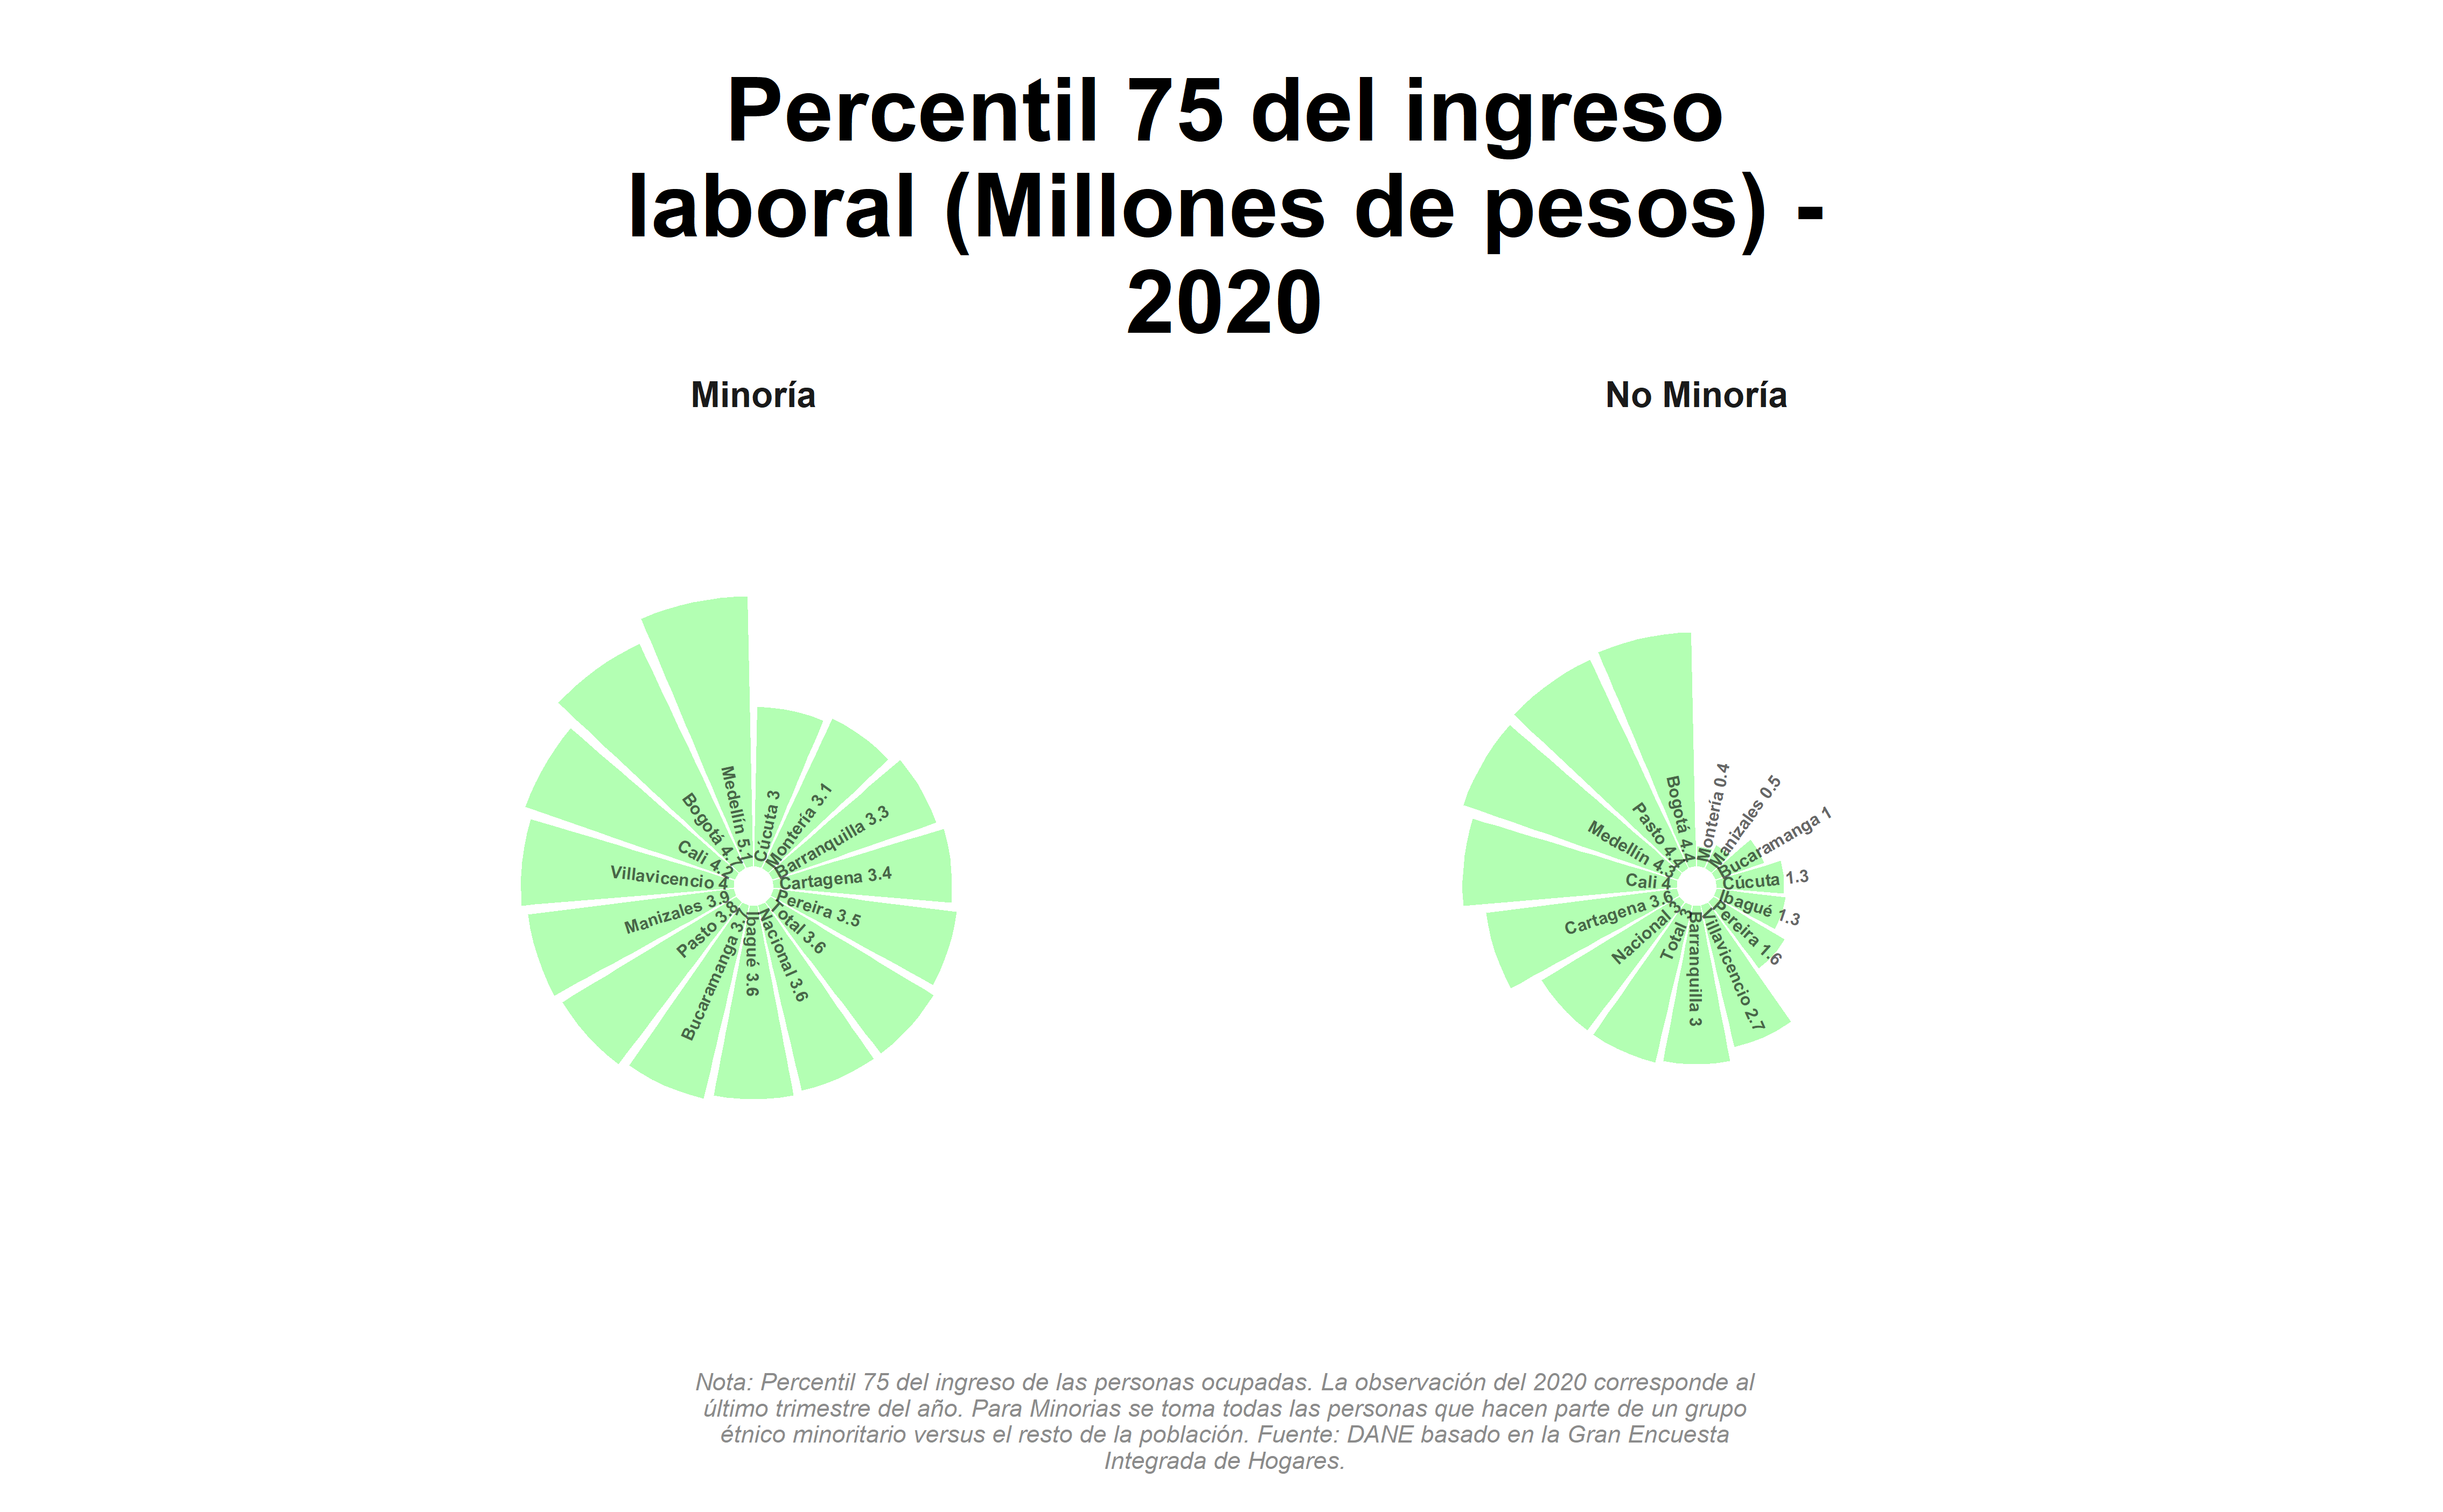
\includegraphics[width=\textwidth,keepaspectratio]{img/var_24_static.png}
        \end{center}
    \end{figure}
            \begin{itemize}
                    \item Diferencia en el ingreso medio entre las ciudades extremos es de dos millones para minorías (Cúcuta - Medellín), y cerca de cuatro millones para las no minorías (Montería - Bogotá).
                    \item Solo Cartagena presenta un ingreso medio nacional mayor para las no minorías, el resto tiene el comportamiento contrario, incluido a nivel nacional.
                    \item Al igual que en el percentil 50, el ingreso medio de las minorías se ve más equitativo que el de las no minorías.
                \end{itemize}

%%%% Include figures
    \begin{figure}[H]
        \caption[Percentil 75 del ingreso laboral por ciudades principales - 2010 VS 2019]{\label{ingreso_laboral_75_ciudades_vs} }
        \begin{center}
        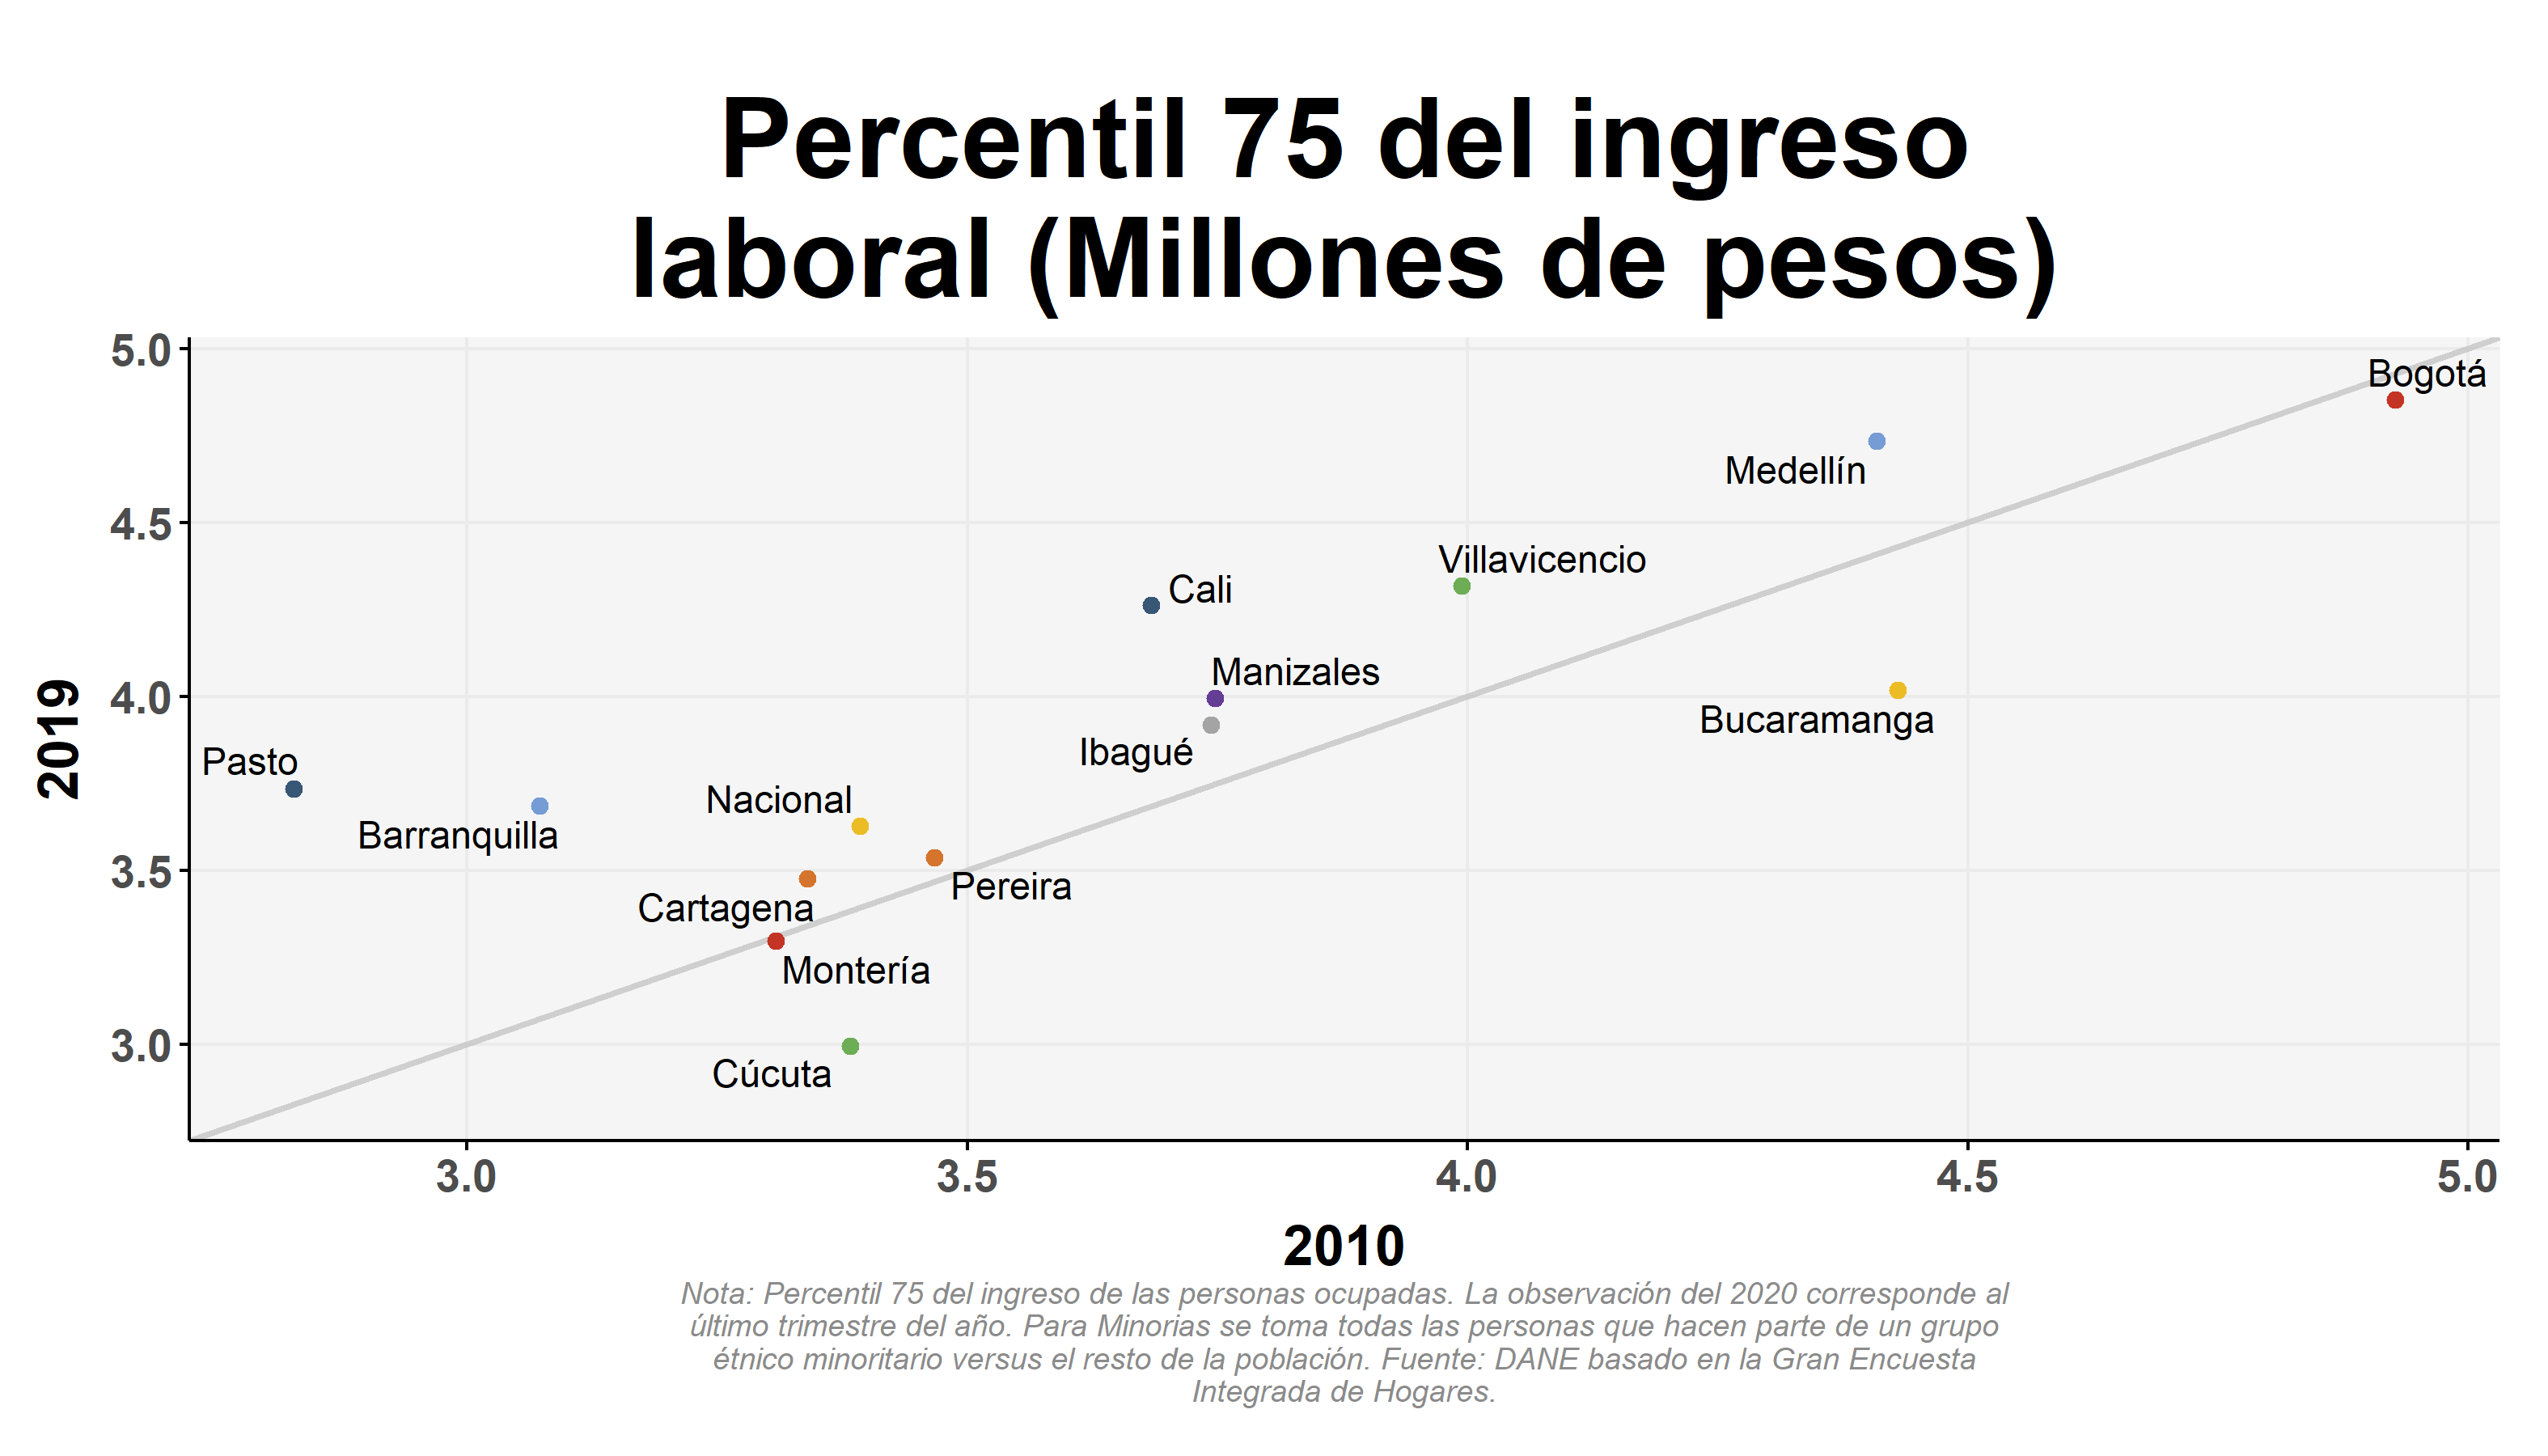
\includegraphics[width=\textwidth,keepaspectratio]{img/var_26455_scatter_time.png}
        \end{center}
    \end{figure}
            \begin{itemize}
                    \item Cúcuta, Bucaramanga y Bogotá son las ciudades donde el ingreso laboral en el percentil 75 disminuyó, siendo Cúcuta y Bucaramanga fueron las que tuvieron la mayor disminución.
                    \item Las demás ciudades aumentaron el ingreso laboral, en especial Pasto que pasó de tener el ingreso más bajo en 2010 a estar en el promedio nacional.
                    \item Montería mantuvo para 2019 el ingreso laboral que registró en 2010.
                \end{itemize}

%%%% Include figures
    \begin{figure}[H]
        \caption[Percentil 75 del ingreso laboral por género ]{\label{ingreso_laboral_75_genero} }
        \begin{center}
        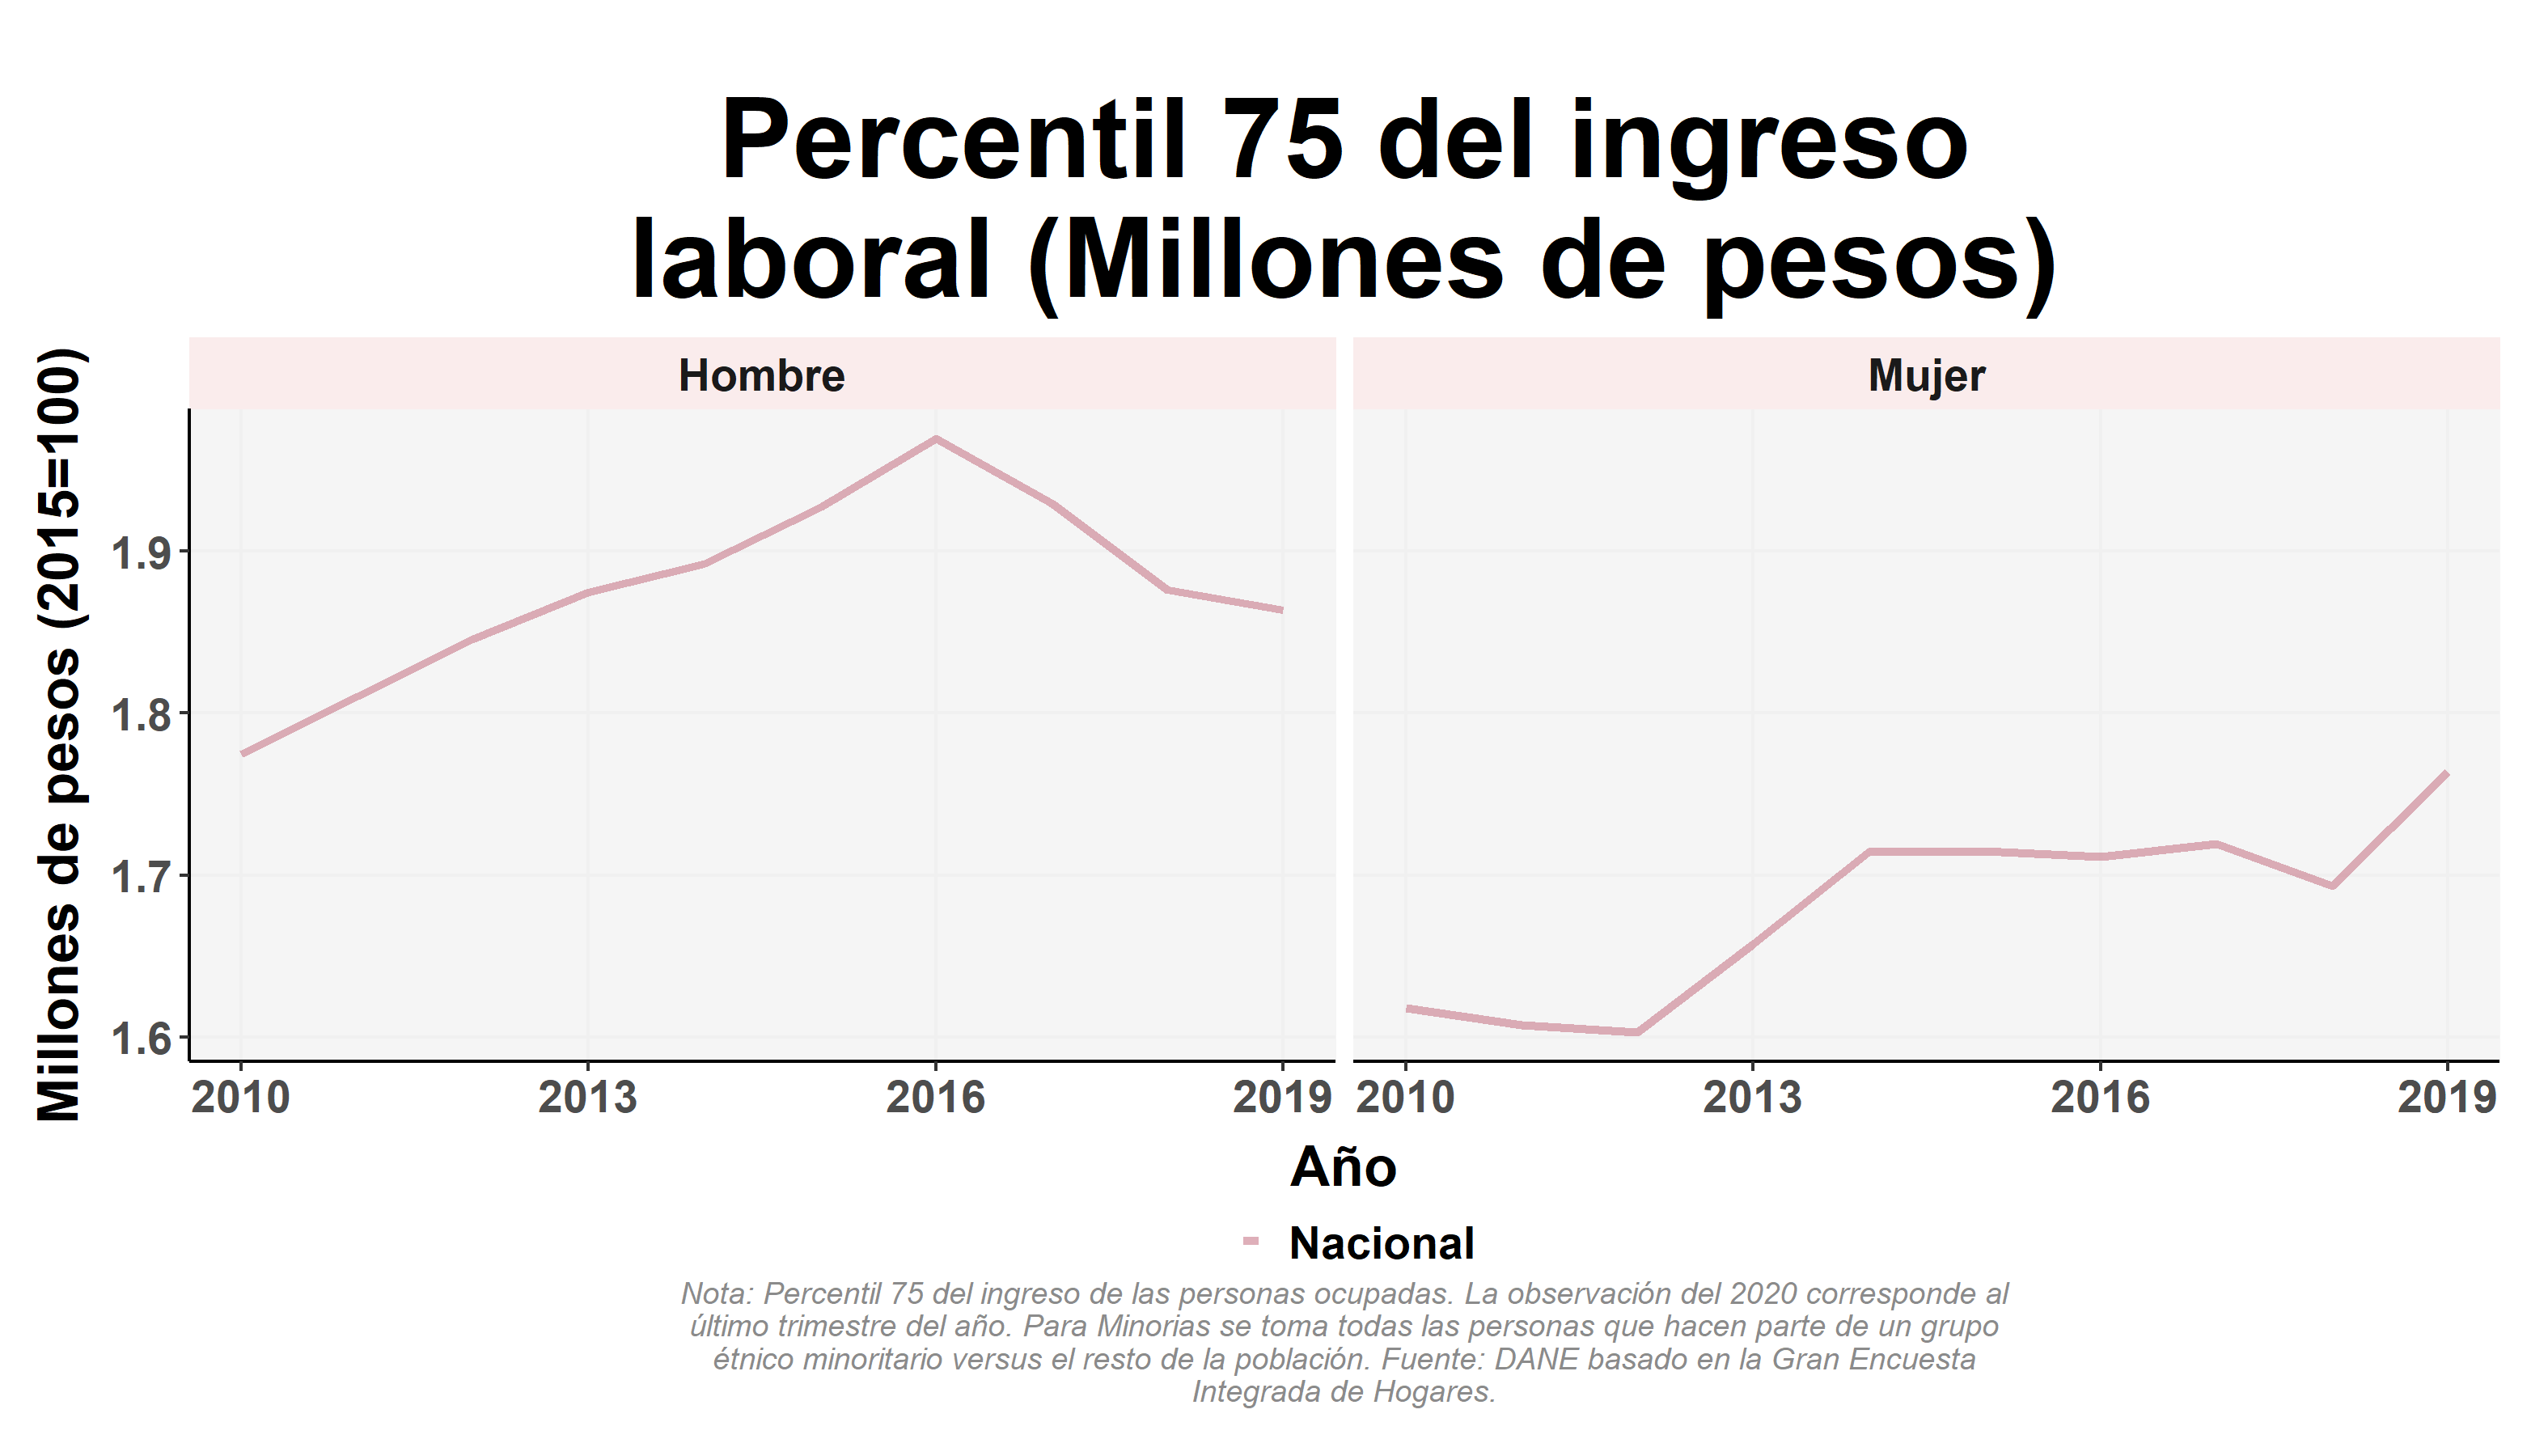
\includegraphics[width=\textwidth,keepaspectratio]{img/var_26_trend.png}
        \end{center}
    \end{figure}
            \begin{itemize}
                    \item En el percentil 75 la brecha de ingreso medio entre géneros ha disminuido, pero aún es persistente, siendo la mujer de menor ingreso.
                    \item El ingreso medio de los hombres en el percentil 75 ha venido disminuyendo desde el 2016.
                    \item En el caso de la mujer el ingreso no ha aumentado significativamente, manteniendo el ingreso en 2019 igual al percibido por un hombre en 2010.
                \end{itemize}

%%%% Include figures
    \begin{figure}[H]
        \caption[Percentil 75 del ingreso laboral nacional ]{\label{ingreso_laboral_75_nacional} }
        \begin{center}
        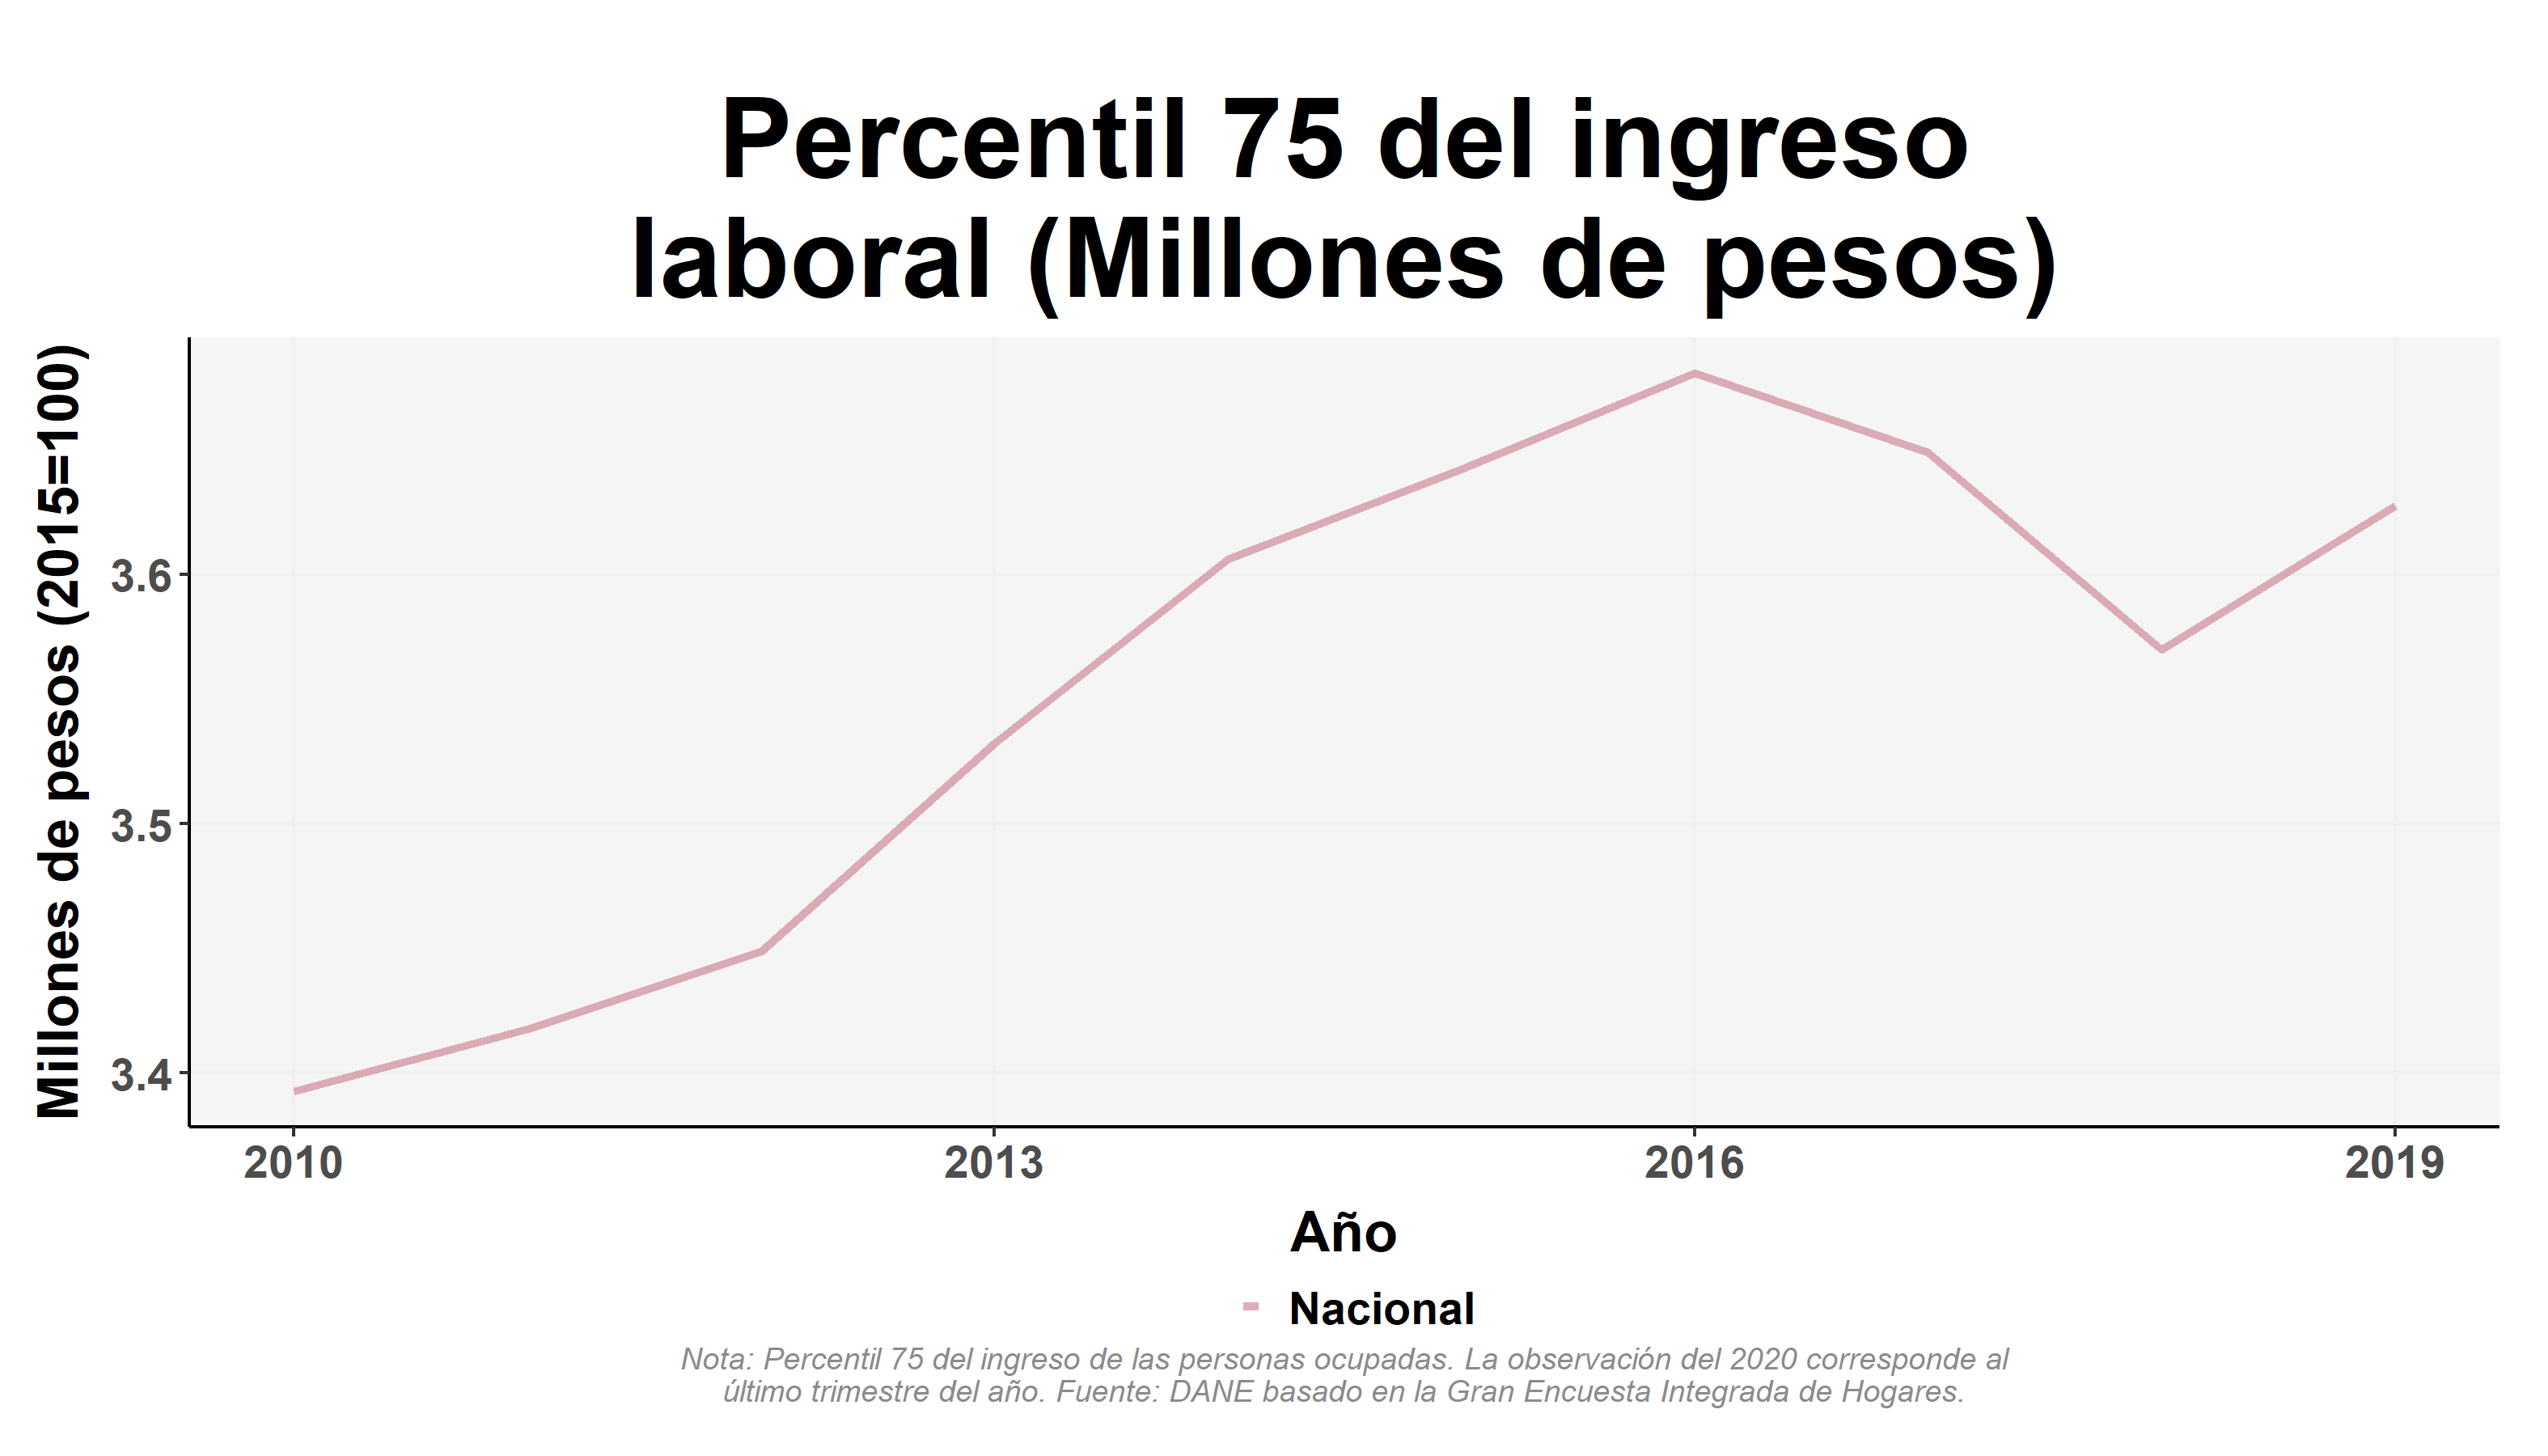
\includegraphics[width=\textwidth,keepaspectratio]{img/var_27_trend.png}
        \end{center}
    \end{figure}
            \begin{itemize}
                    \item El ingreso medio nacional en el percentil 75 tuvo crecimiento constante hasta el 2016 donde empezó a disminuir hasta el 2017 donde vuelve a verse un aumento para el 2019.
                    \item Este comportamiento se asemeja al de los hombres para el percentil 75.
                \end{itemize}

\section{Pobreza}

    \begin{figure}[H]
        \caption[Indicador Pulso Social sobre Pobreza (PCA)]{\label{pca_pobreza} }
        \begin{center}
        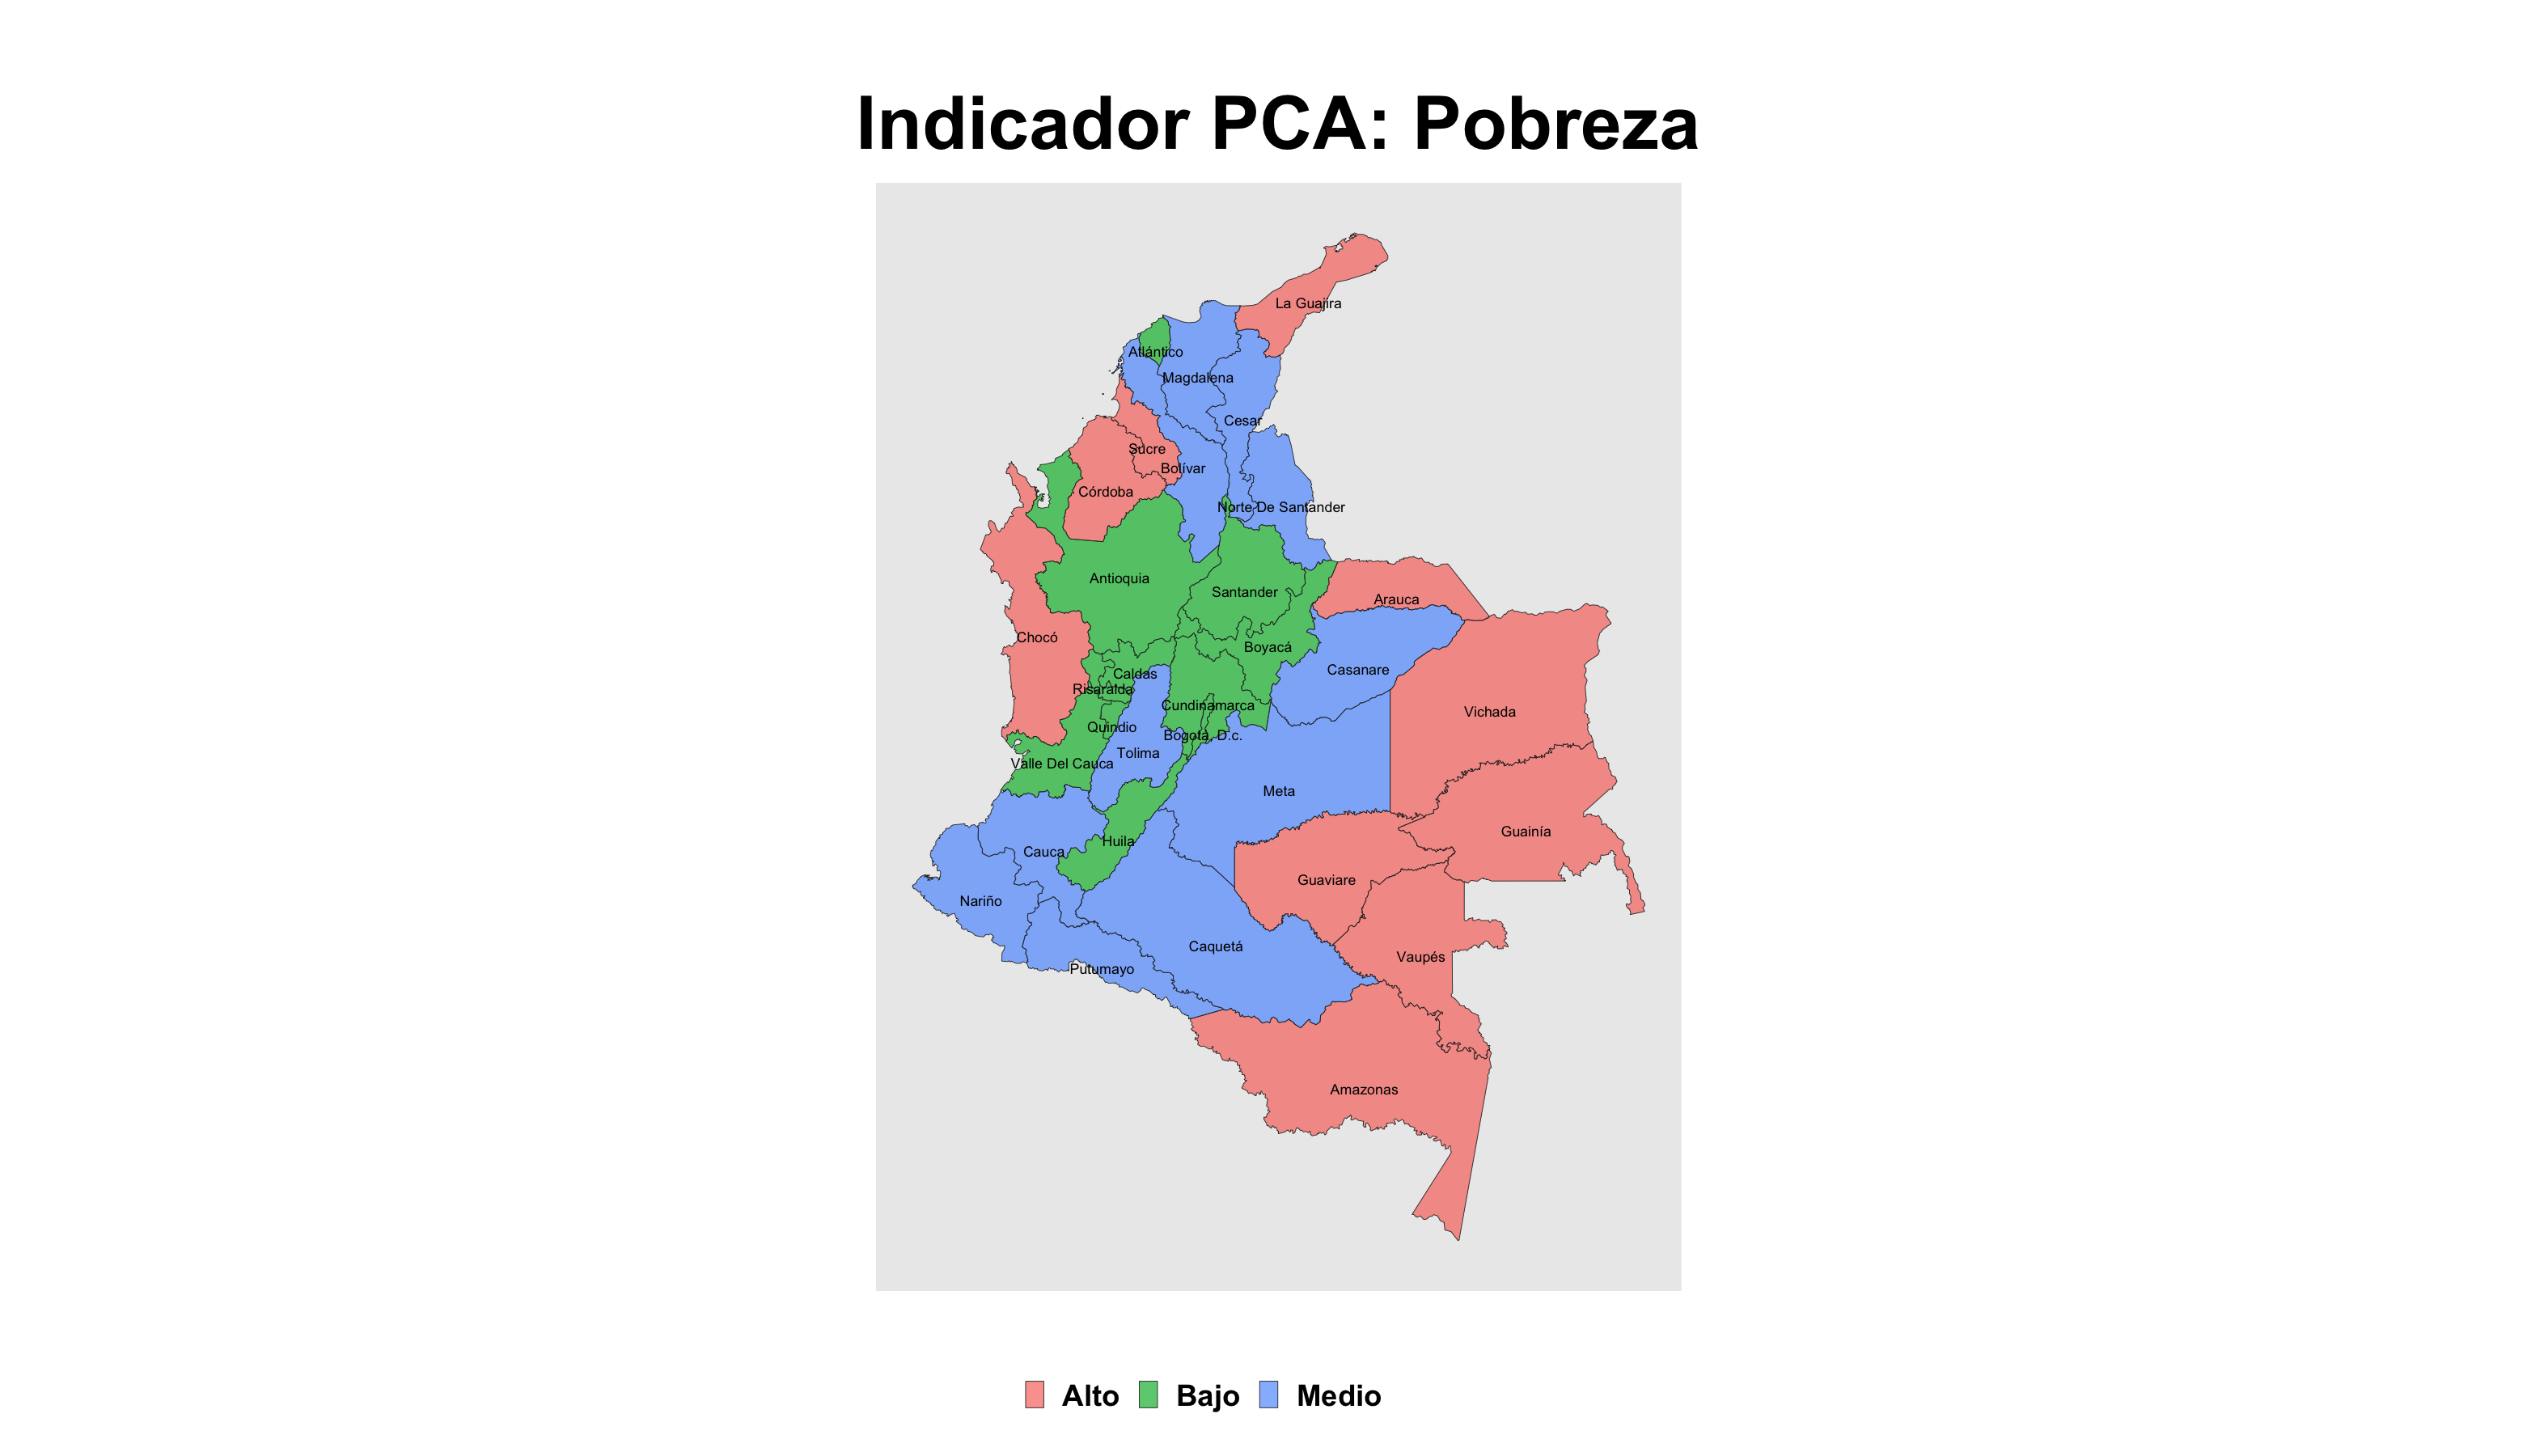
\includegraphics[width=\textwidth,keepaspectratio]{pca_clusters/pca_pobreza_pca.png}
        \end{center}
    \end{figure}

 %%%%---------------------
    %%% Principales resultados
    %%%%---------------------
    \begin{tcolorbox}[enhanced, colback=mycolor,colframe=mycolor,drop fuzzy shadow,watermark color=white,
                        %%% Título
                        title=Principales Resultados]
    
                    \begin{itemize}
                    \item Pero hay una brecha de género enorme, especialmente en los percentiles más bajos de ingreso.
                    \item El rezago en el ingreso de las mujeres con respecto al de los hombres es de más de 10 años.
                \end{itemize}
     
    \end{tcolorbox}
    %%%%---------------------
    %%%%---------------------
    %%%%---------------------

    \subsection{Pobreza Monetaria}

        \subsubsection{Población por Clase Social}

%%%% Include figures
    \begin{figure}[H]
        \caption[Población por clase social - Pobres (2012 VS 2020) por ciudad ]{\label{pobres_ciudad_vs} }
        \begin{center}
        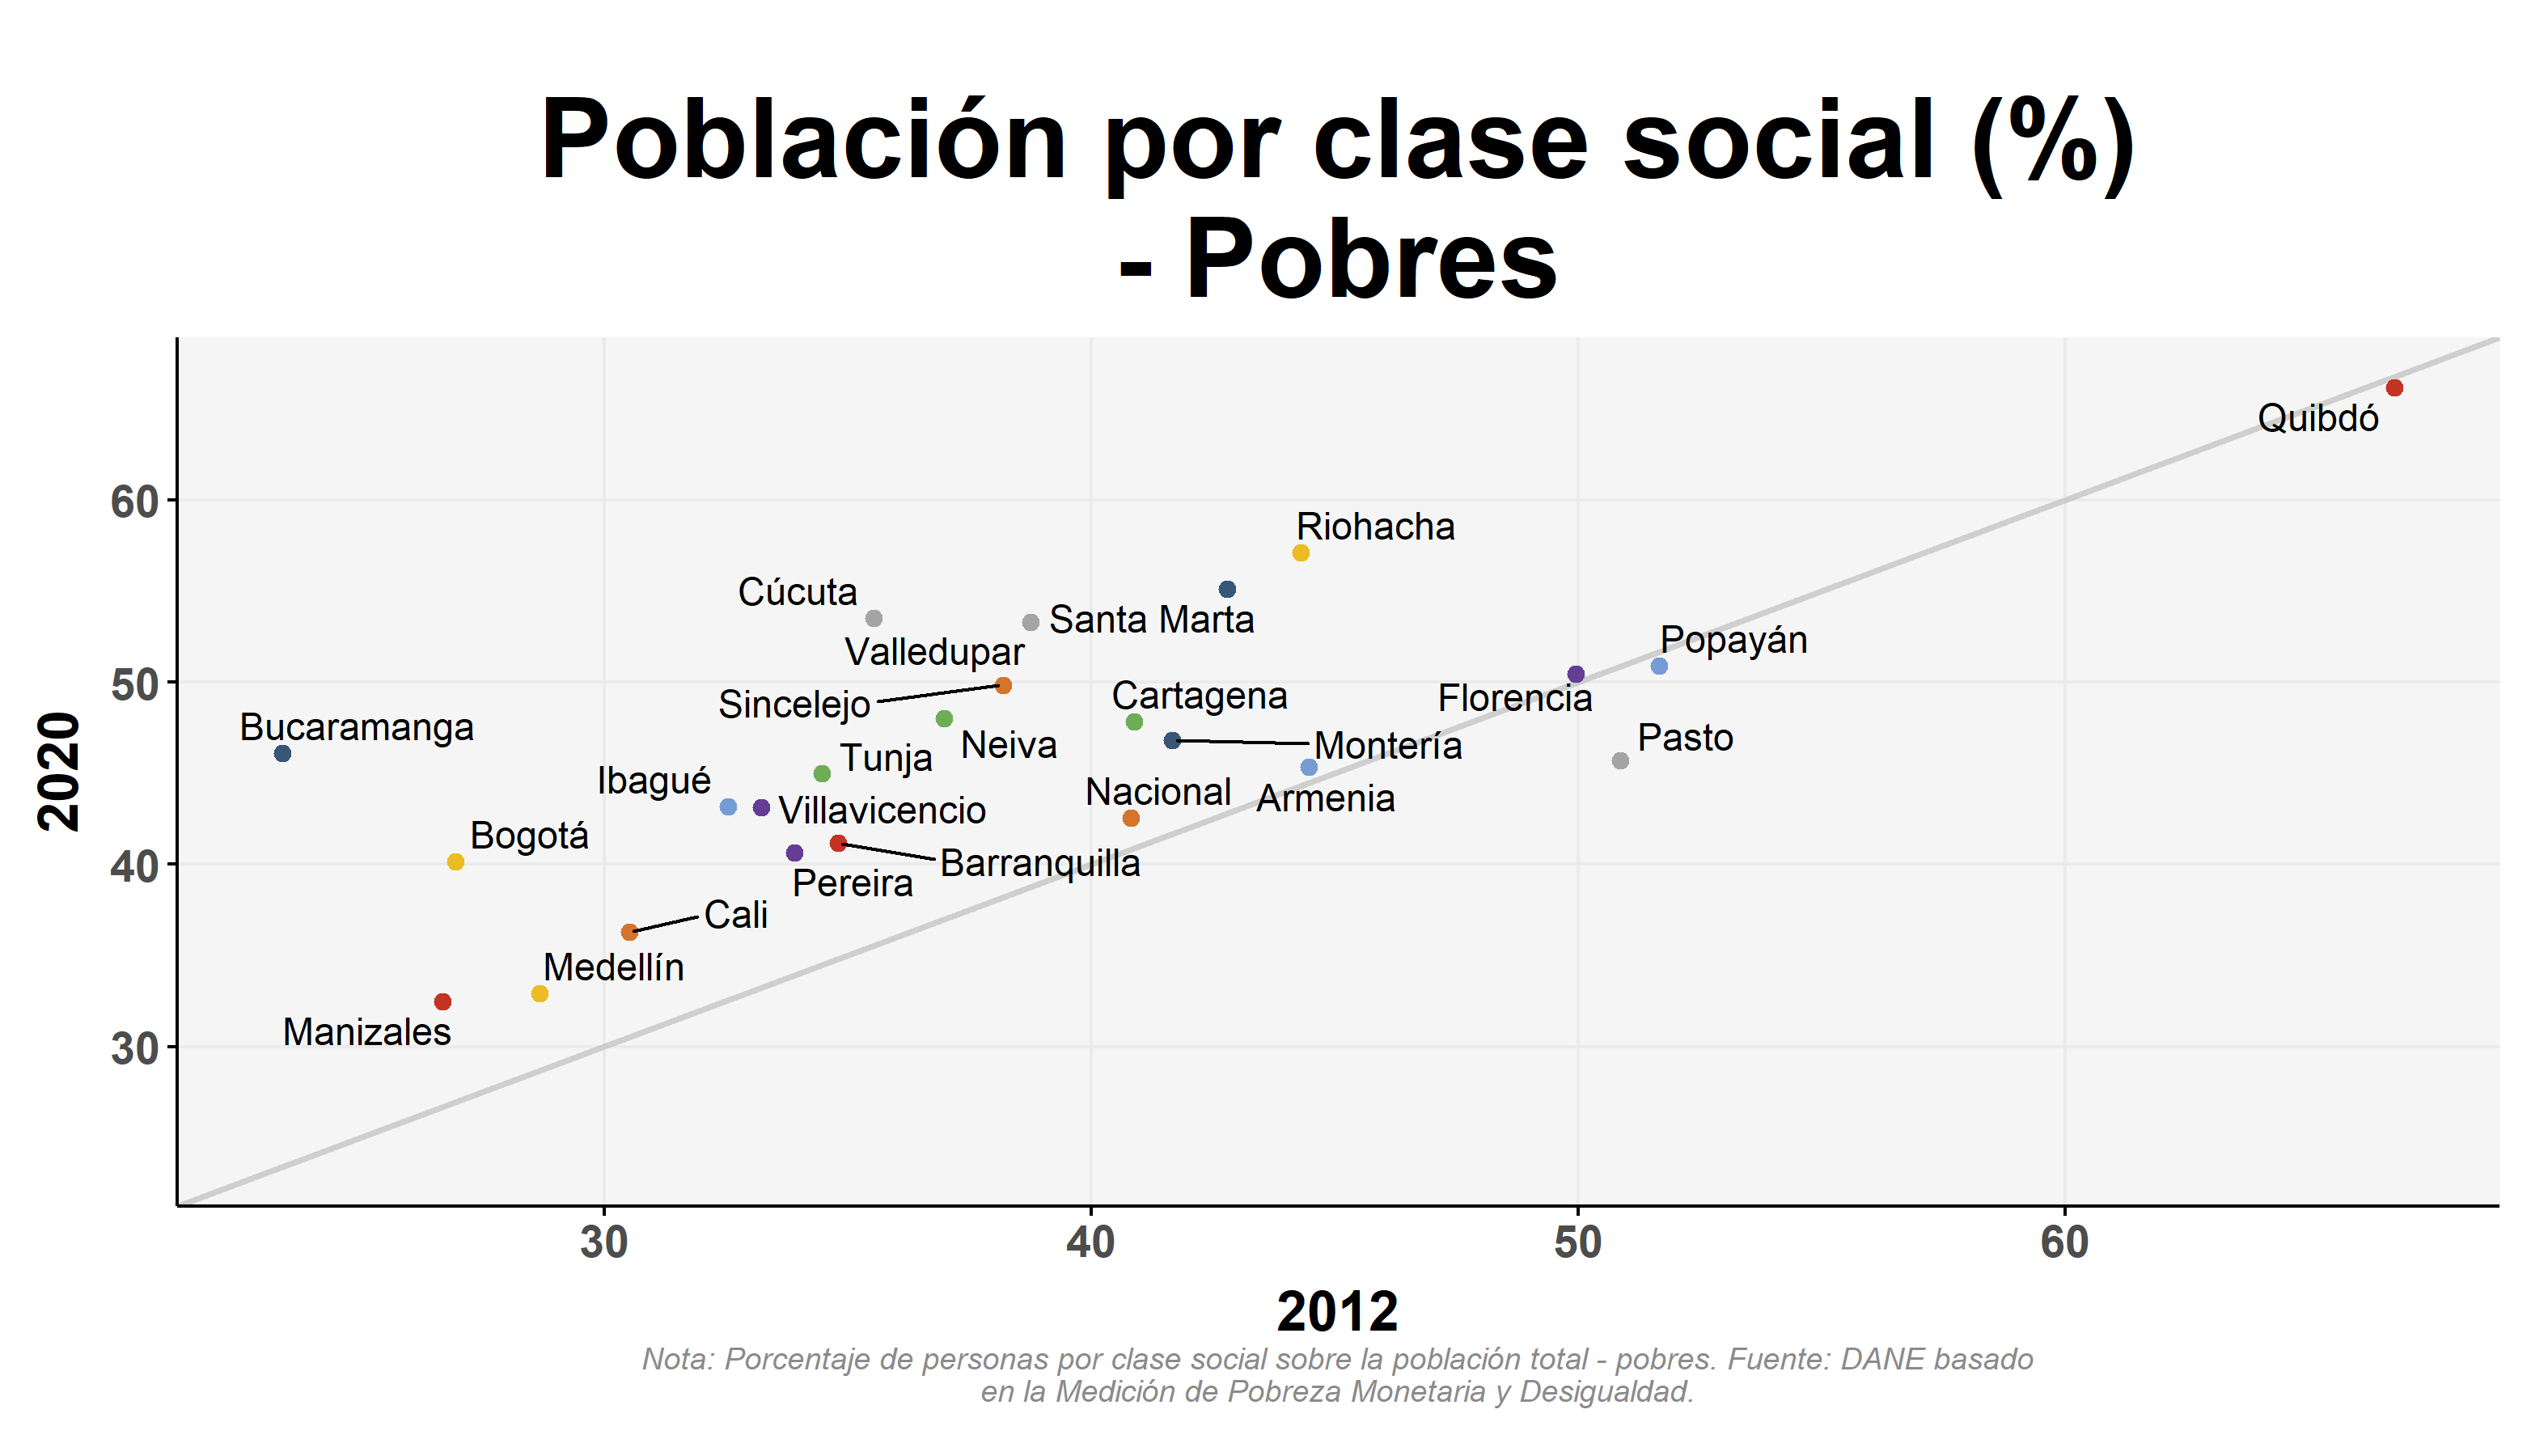
\includegraphics[width=\textwidth,keepaspectratio]{img/var_241_scatter_time.png}
        \end{center}
    \end{figure}
            \begin{itemize}
                    \item Pasto es la única ciudad que disminuyó el porcentaje de pobres entre 2012 y 2020.
                    \item Quibdó, Popayán, Florencia y Armenia mantuvieron el porcentaje de pobres similares entre el 2012 y 2020.
                    \item Gran parte de las ciudades mostraron un aumento en el porcentaje de pobres para el 2020.
                    \item Quibdó sobresale entre las demás ciudades con niveles de pobreza sobre el 60\% y con una diferencia con el segundo de menos del 10\% para 2020, la brecha disminuyó comparado con el 2012 (más del 10\%).
                    \item A nivel nacional la pobreza aumentó levemente.
                    \item Bucaramanga pasó de ser la ciudad con menor porcentaje de pobreza con niveles por debajo del 30\% en 2012 a tener niveles por encima del 45\% para 2020.
                    \item Hay una diferencia de aproximadamente un 30\% entre la ciudad con mayor nivel de pobreza, Quibdó, y la de menor nivel, Manizales, para el 2020 (Se puede evidenciar en el static).
                \end{itemize}

%%%% Include figures
    \begin{figure}[H]
        \caption[Población por clase social - Pobres a nivel nacional ]{\label{pobres_nacional} }
        \begin{center}
        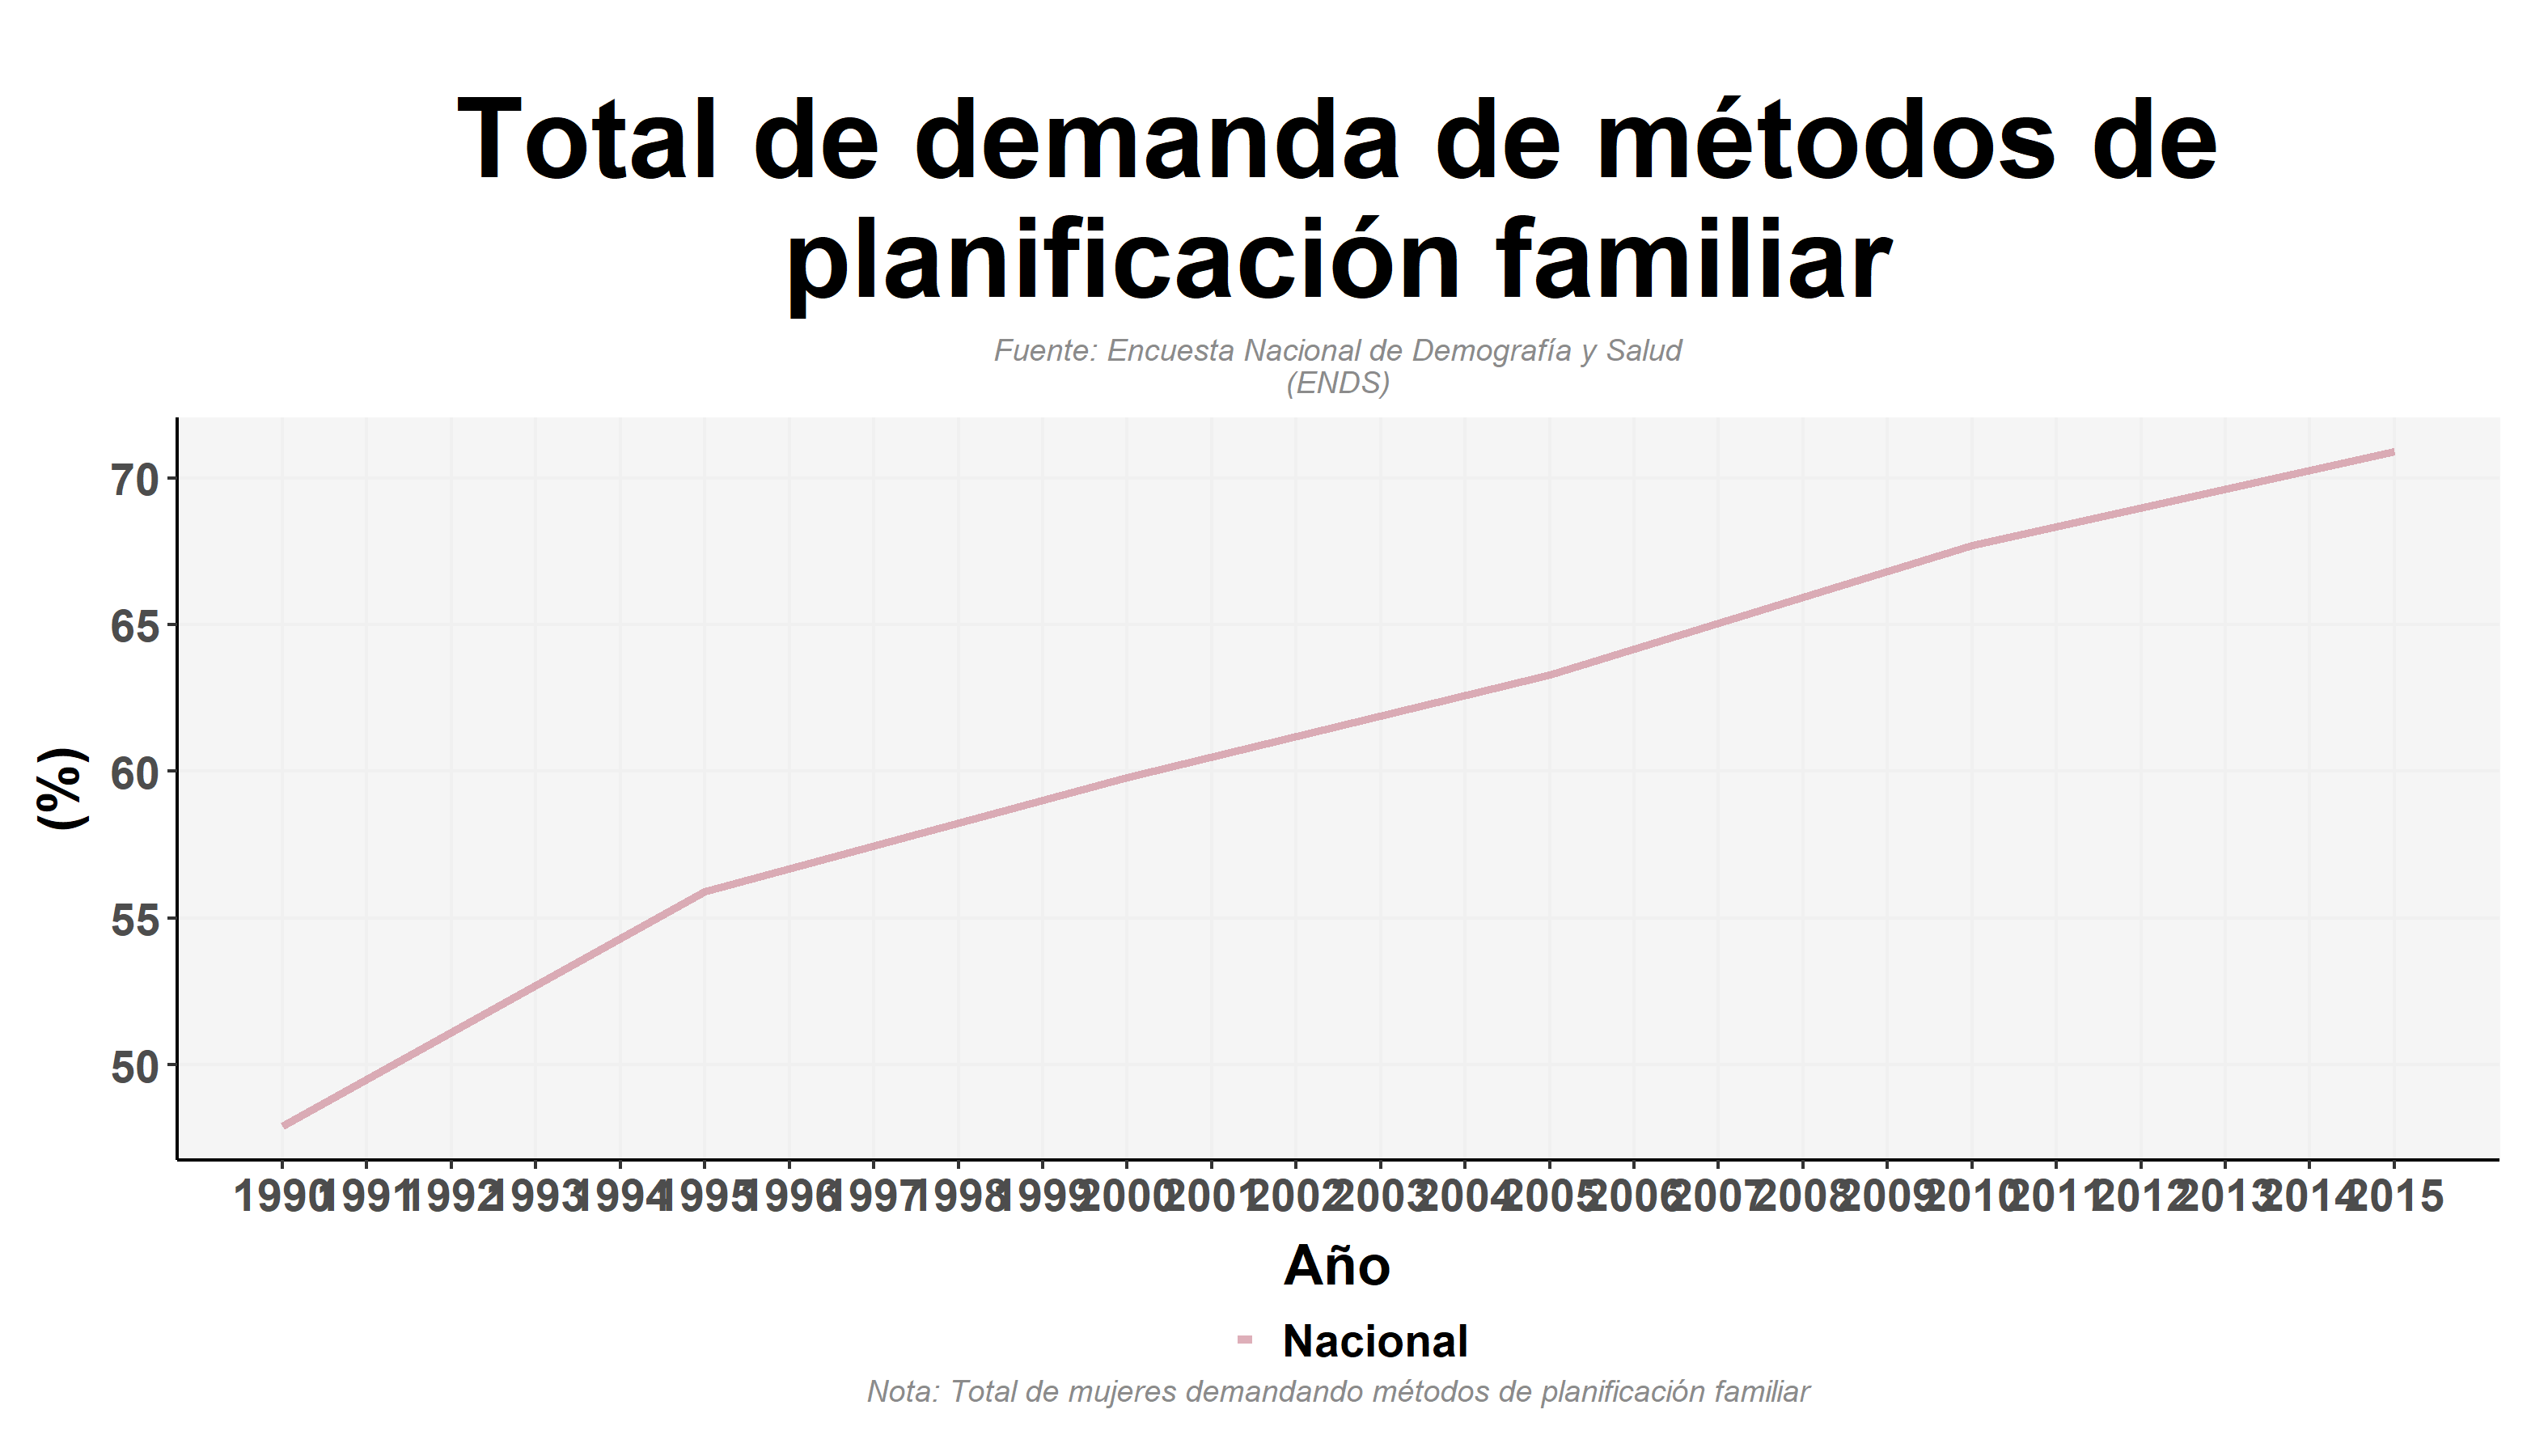
\includegraphics[width=\textwidth,keepaspectratio]{img/var_242_trend.png}
        \end{center}
    \end{figure}
            \begin{itemize}
                    \item El porcentaje de pobres venía disminuyendo a partir del 2012 hasta el 2018, donde empieza a aumentar.
                    \item A partir de 2019 empieza a aumentar el porcentaje de pobreza, y se intensifica en el 2020 superando los niveles del 2012.
                    \end{itemize}

%%%% Include figures
    \begin{figure}[H]
        \caption[Población por clase social - Pobres por zonas ]{\label{pobres_zonas} }
        \begin{center}
        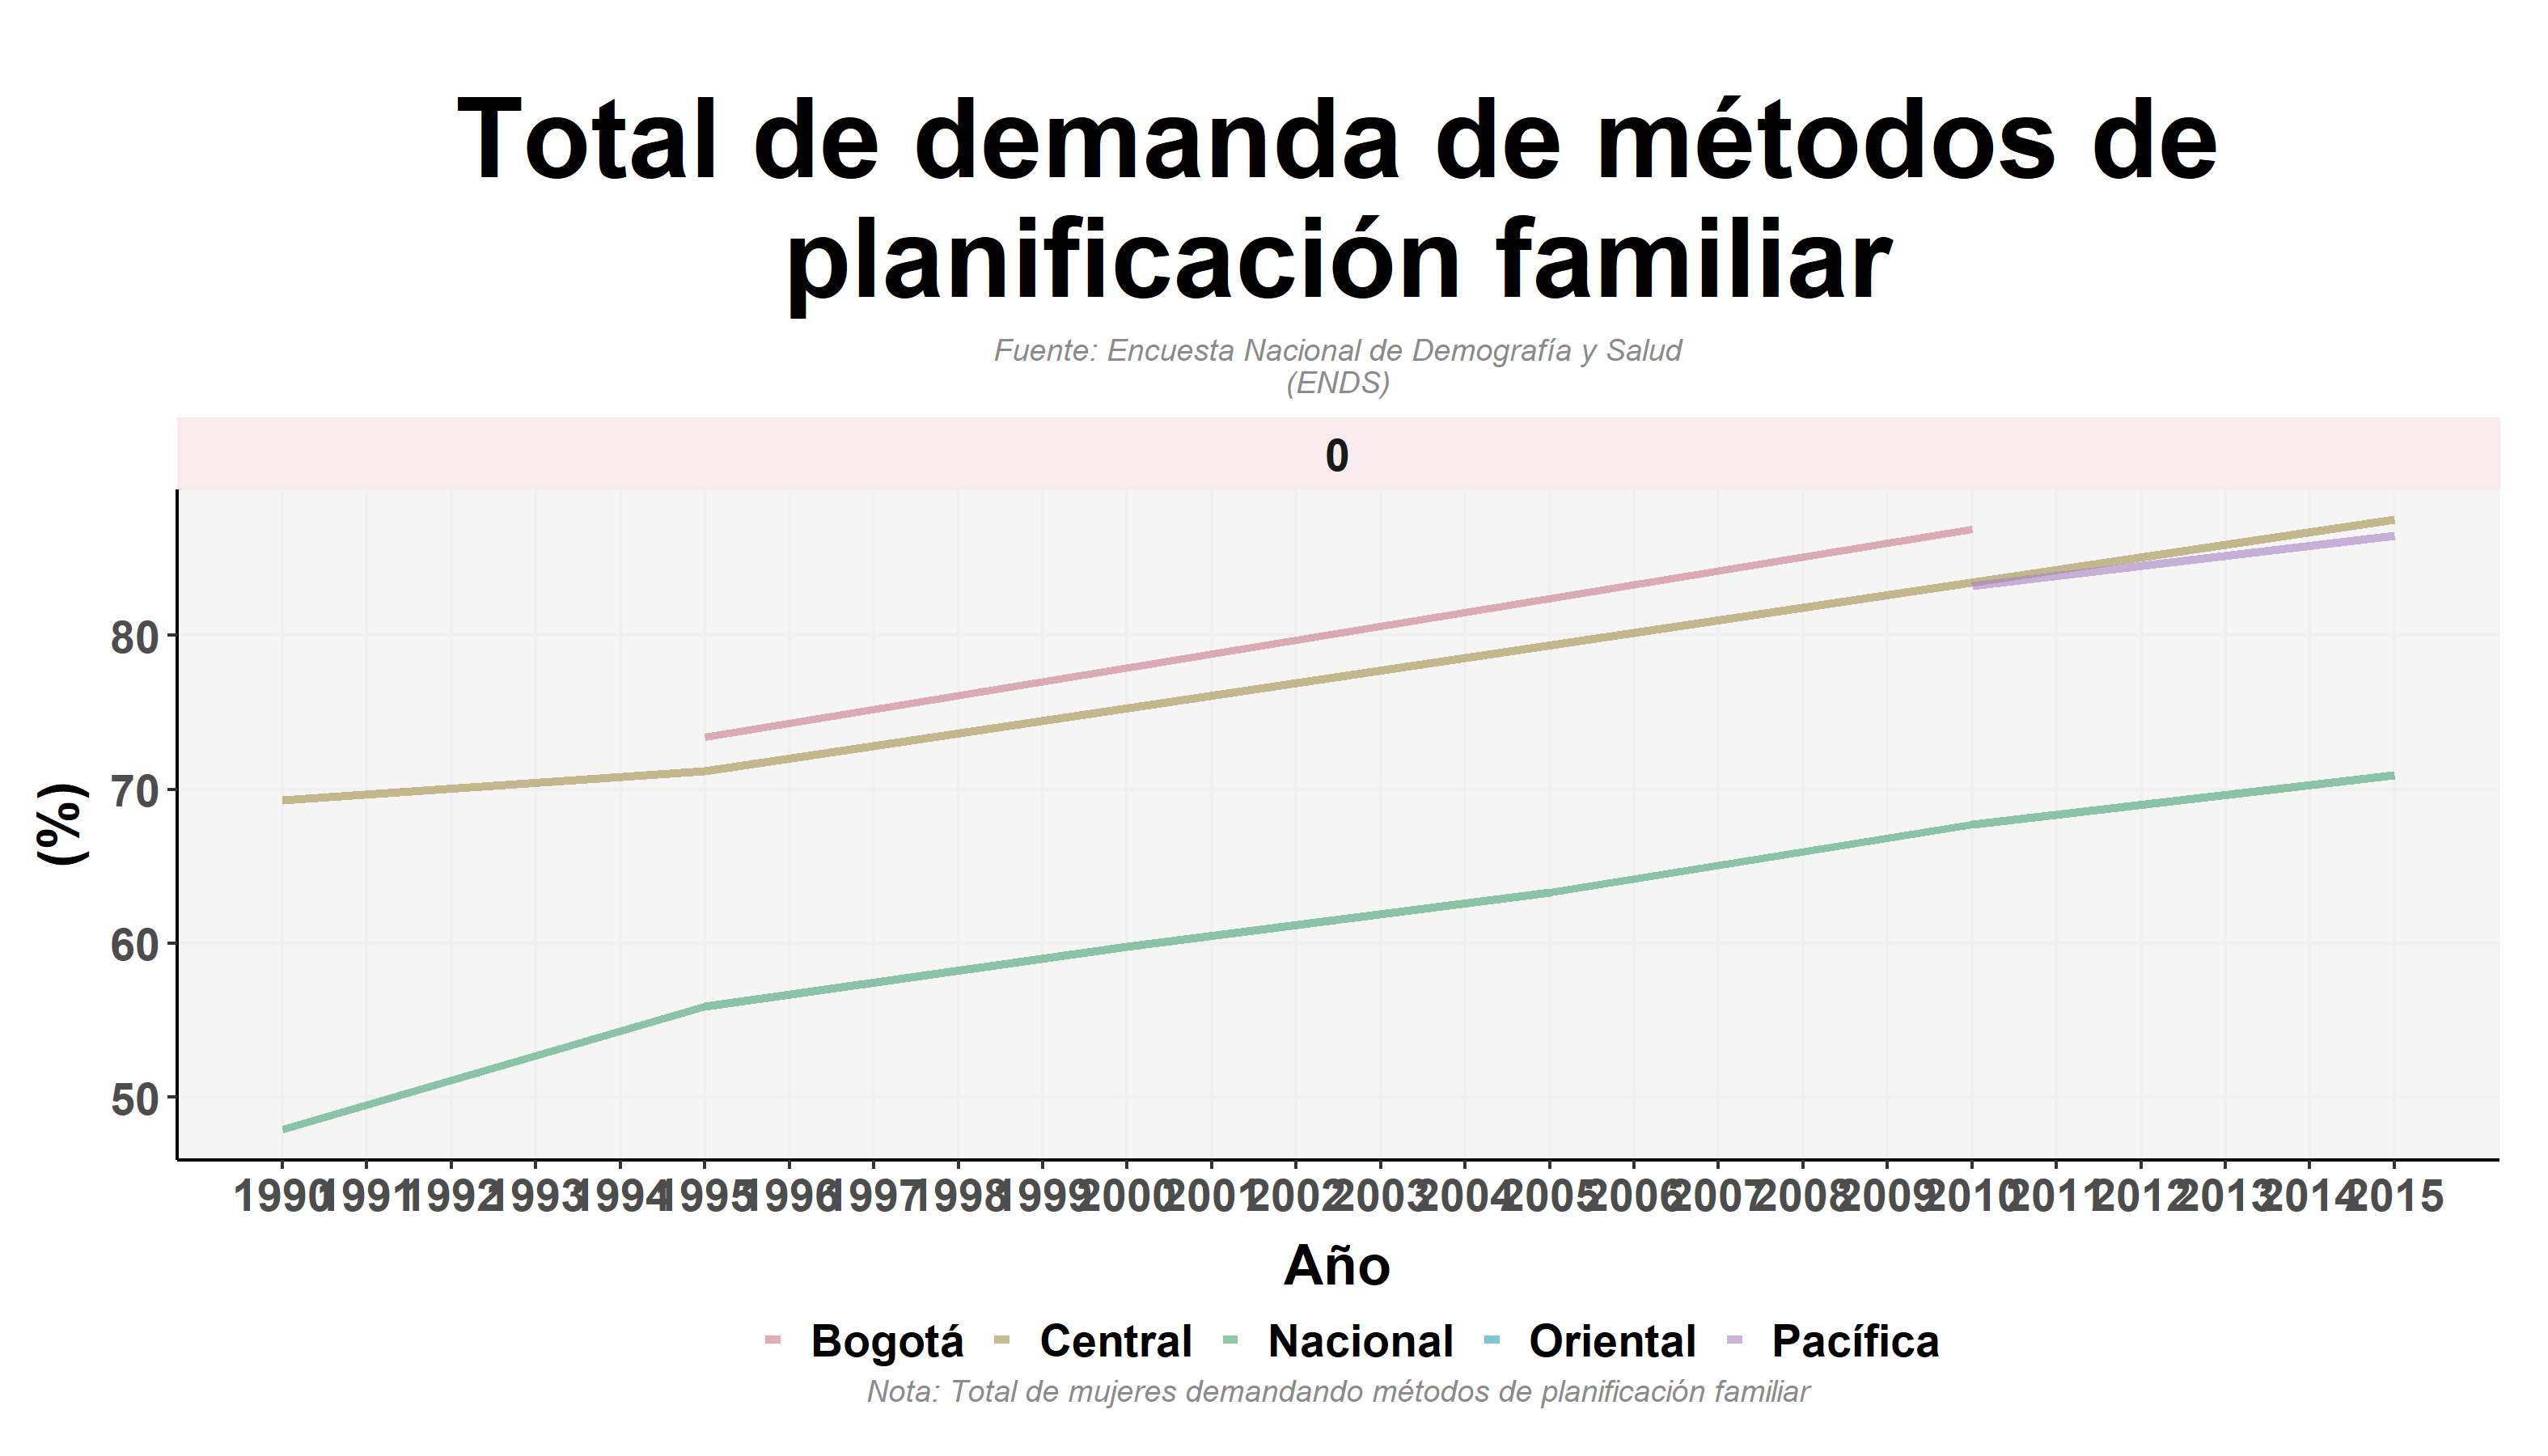
\includegraphics[width=\textwidth,keepaspectratio]{img/var_243_trend.png}
        \end{center}
    \end{figure}
            \begin{itemize}
                    \item Mientras que los niveles de pobreza aumentaron a nivel nacional y en las cabeceras, en los centros poblados y rural disperso esta disminuyó.
                    \item Los niveles de pobreza en las cabeceras y en las zonas rurales pasaron de tener brechas del más del 10\% hasta el 2019 a estar a niveles similares en el 2020.
                    \item El porcentaje de pobres a nivel nacional y en cabeceras tiene niveles superiores a los del 2012.
                    \end{itemize}

%%%% Include figures
    \begin{figure}[H]
        \caption[Población por clase social - Vulnerables (2012 VS 2020) por ciudad ]{\label{vulnerables_ciudades_vs} }
        \begin{center}
        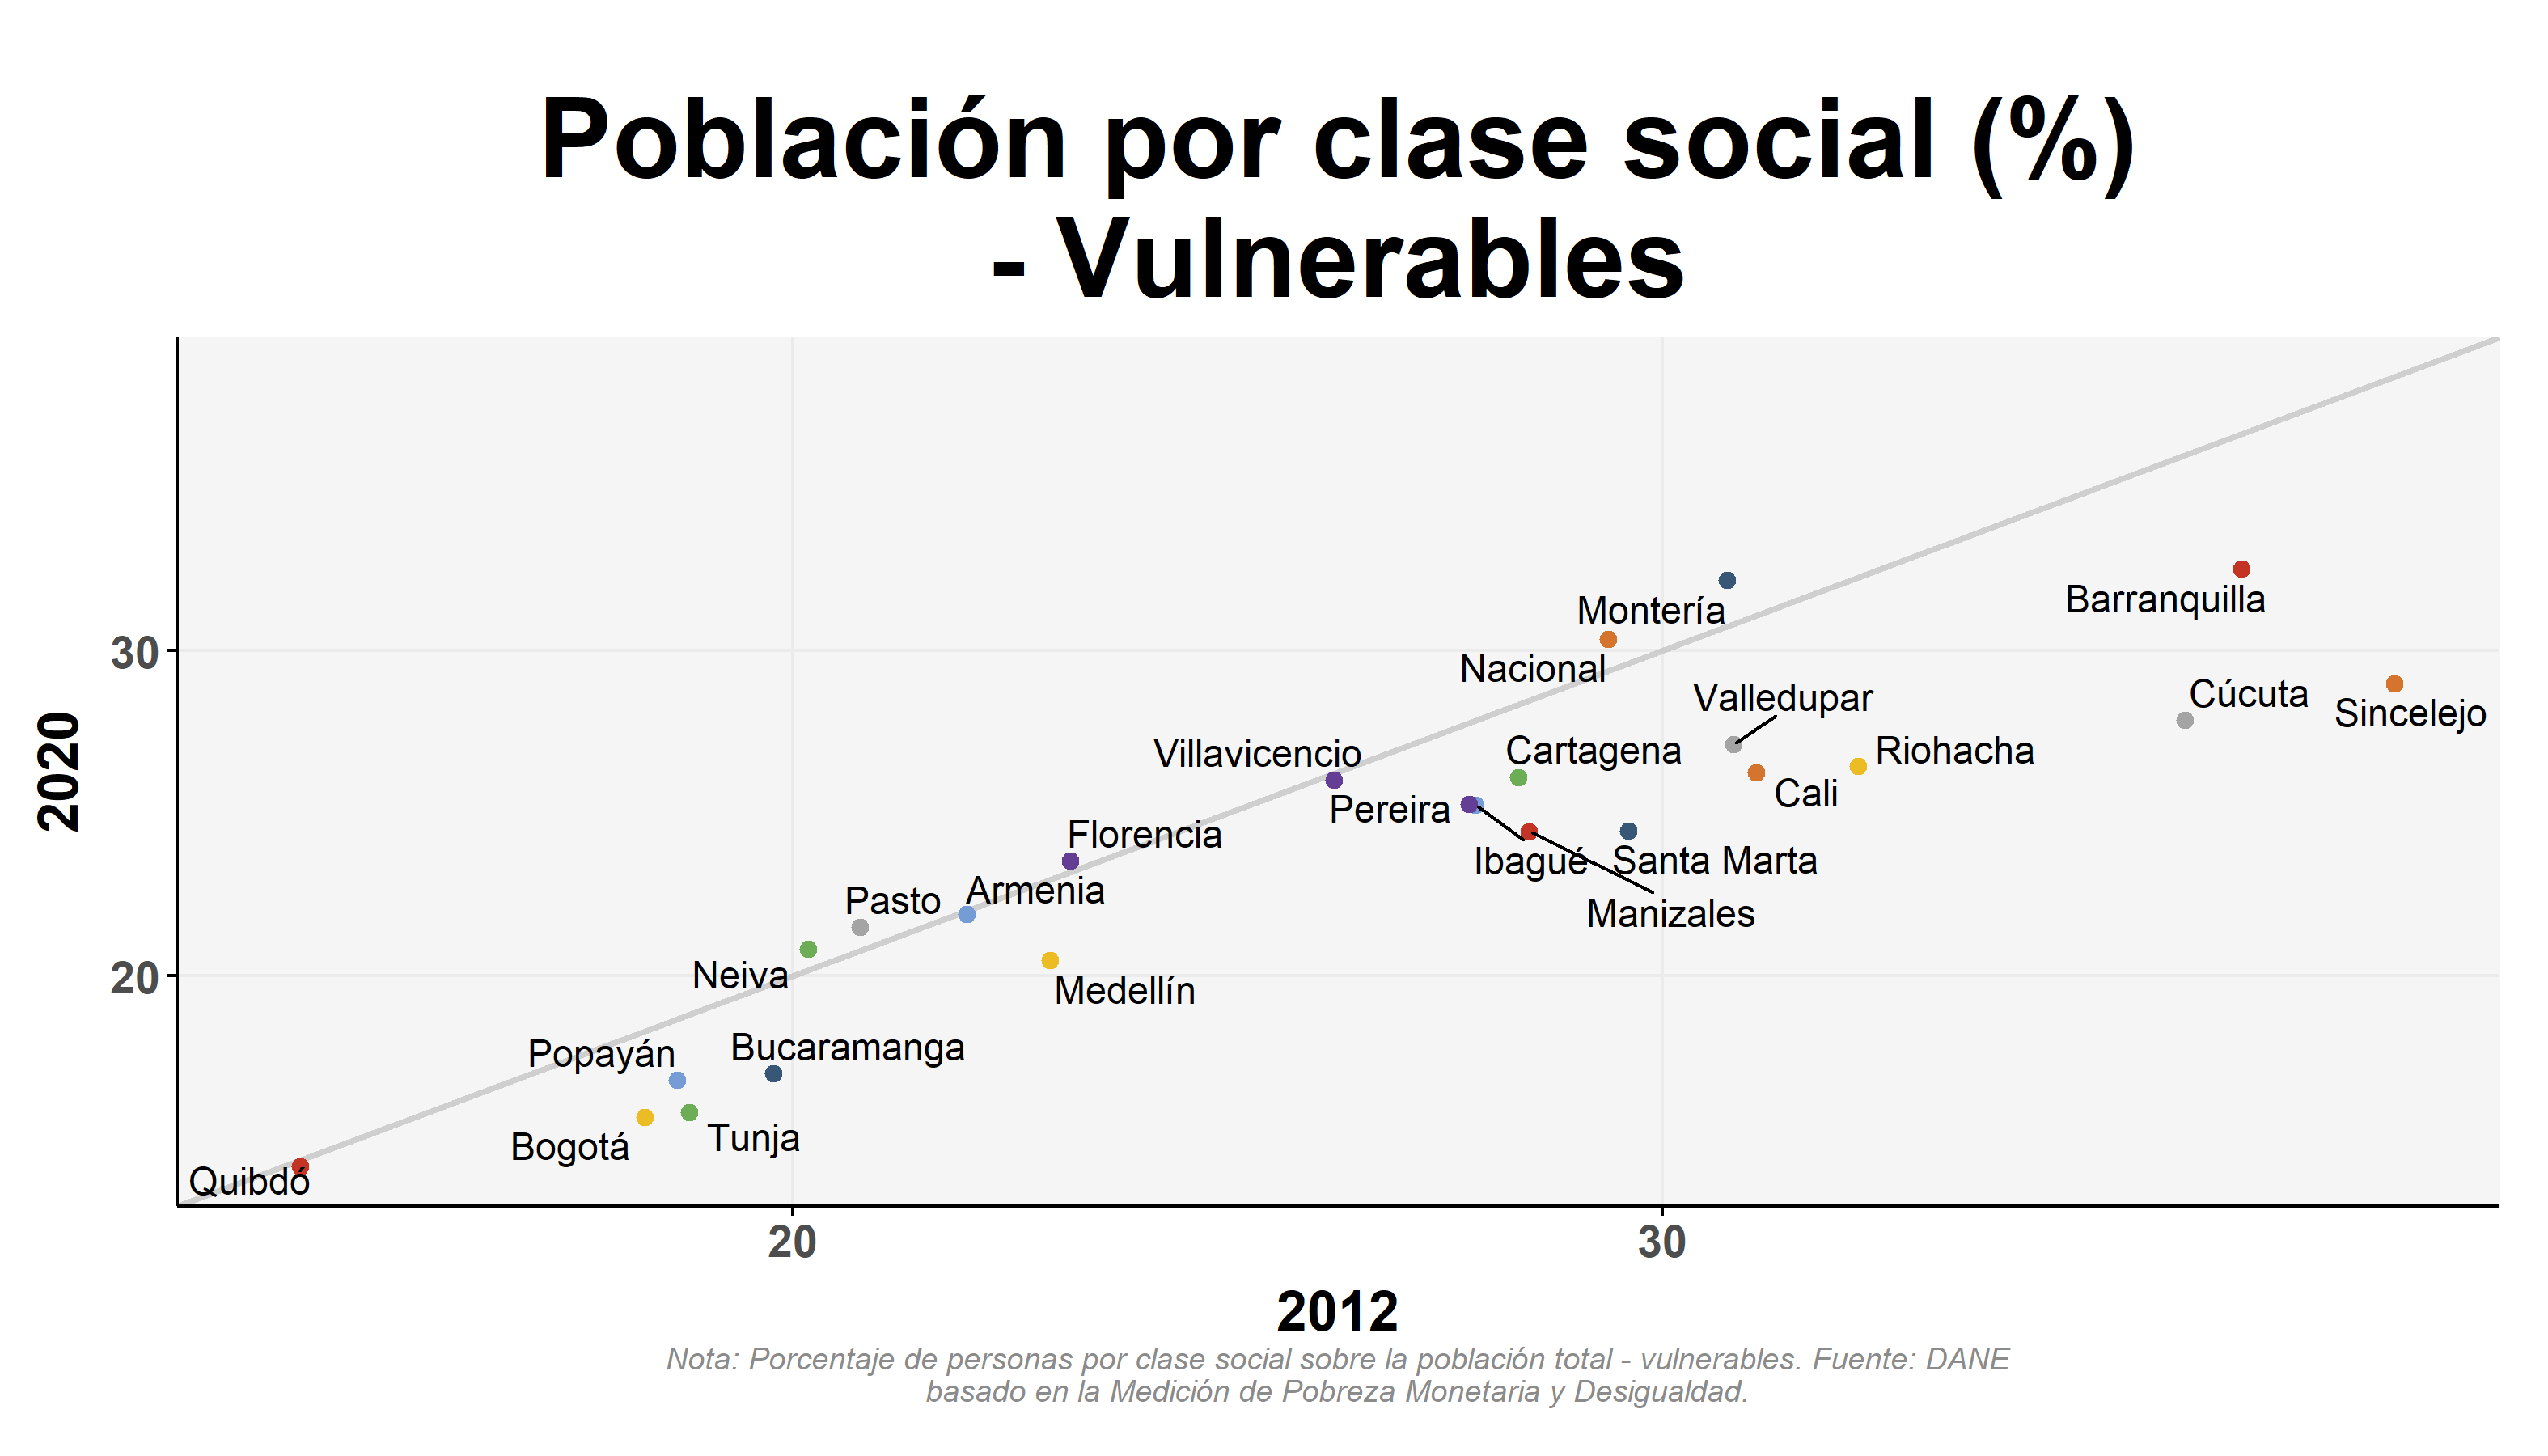
\includegraphics[width=\textwidth,keepaspectratio]{img/var_244_scatter_time.png}
        \end{center}
    \end{figure}
            \begin{itemize}
                    \item El porcentaje de vulnerables ha disminuido entre 2012 y 2020 en gran parte de las ciudades principales.
                    \item Ciudades como Villavicencio, Florencia, Quibdó y Armenia se mantienen a los mismos niveles de 2012.
                    \item A nivel nacional el porcentaje de vulnerables aumentó con respecto al 2012 levemente para el 2020.
                    \item Quibdó para ambos años de referencia es el de menor porcentaje de vulnerables.
                    \item La diferencia entre la ciudad con mayor nivel de población vulnerable (Barranquilla) y la de menor nivel de población (Quibdó) es de alrededor de 15\%.
                    \end{itemize}

%%%% Include figures
    \begin{figure}[H]
        \caption[Población por clase social - Vulnerables a nivel nacional ]{\label{vulnerables_nacional} }
        \begin{center}
        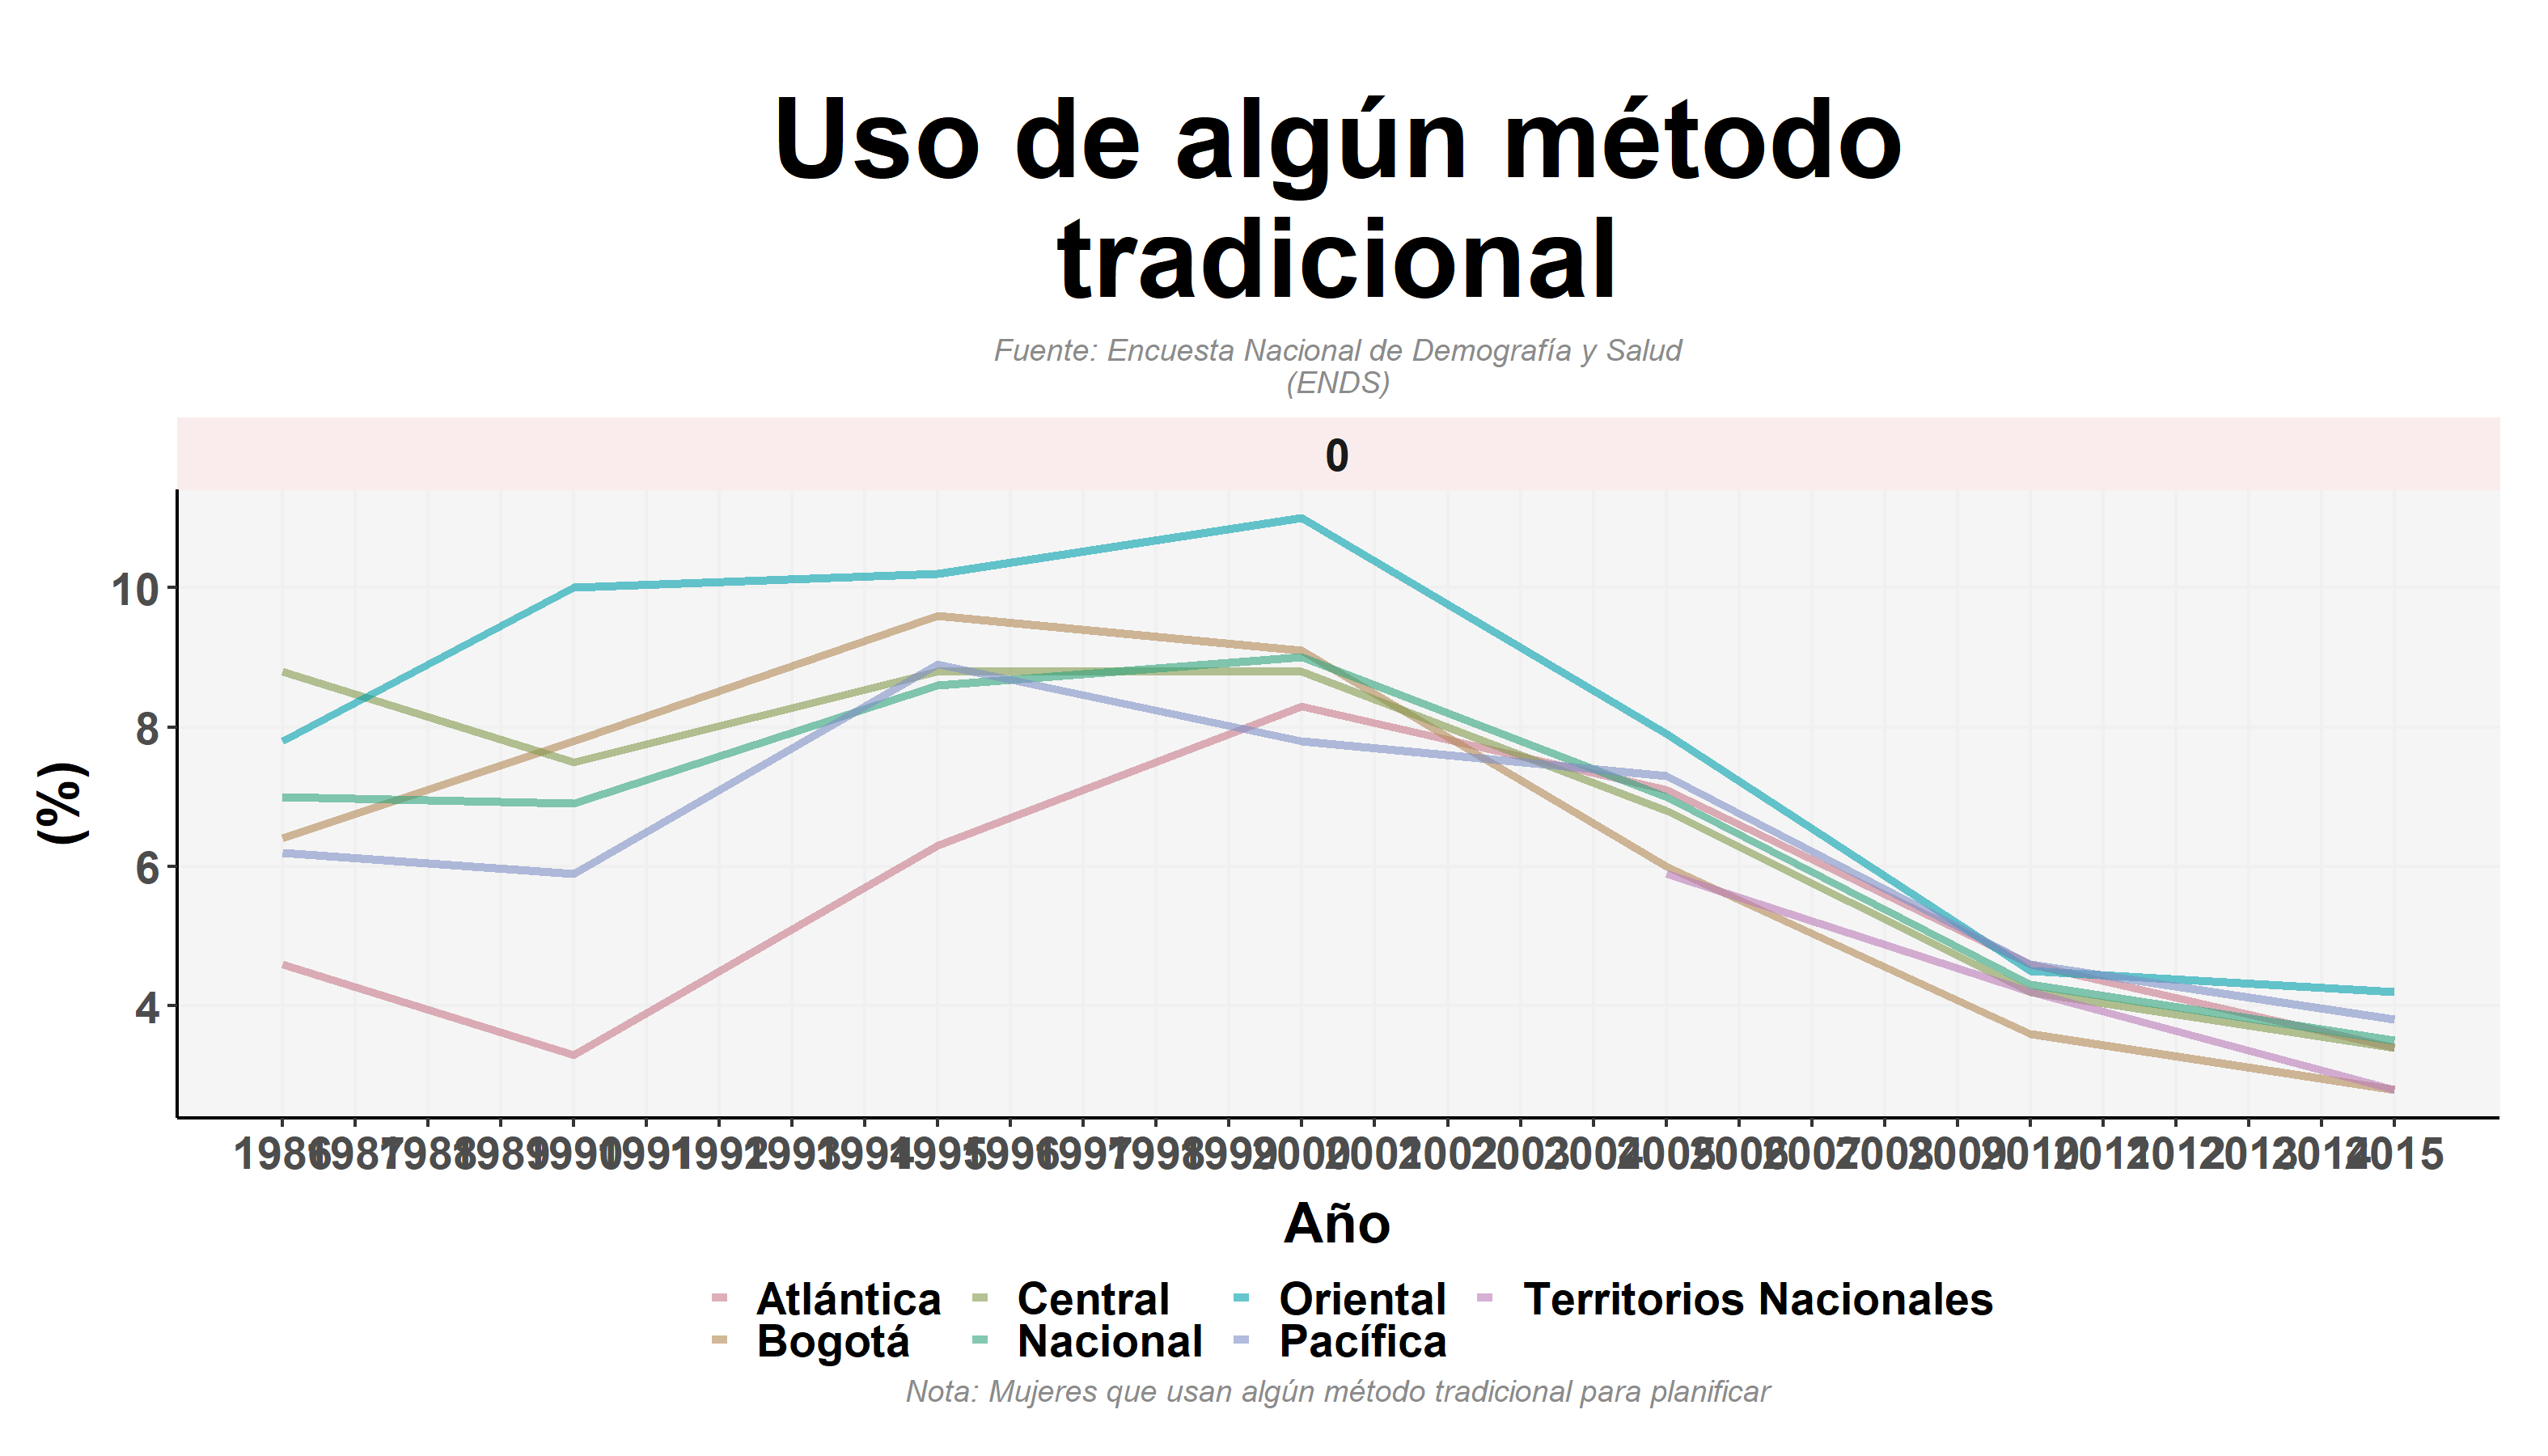
\includegraphics[width=\textwidth,keepaspectratio]{img/var_245_trend.png}
        \end{center}
    \end{figure}
            \begin{itemize}
                    \item El porcentaje de vulnerables estaba aumentando hasta 2018, a partir de ahí empieza a decaer intensificándose en el 2020.
                    \item Para 2020 el porcentaje de vulnerables tiene un retroceso cercano a los niveles del 2013.
                    \item Para el 2016 el porcentaje de vulnerables disminuyó con respecto al año anterior, pero se recuperó y aumentó en el año siguiente.
                    \end{itemize}

%%%% Include figures
    \begin{figure}[H]
        \caption[Población por clase social - Vulnerables por zonas ]{\label{vulnerables_zonas} }
        \begin{center}
        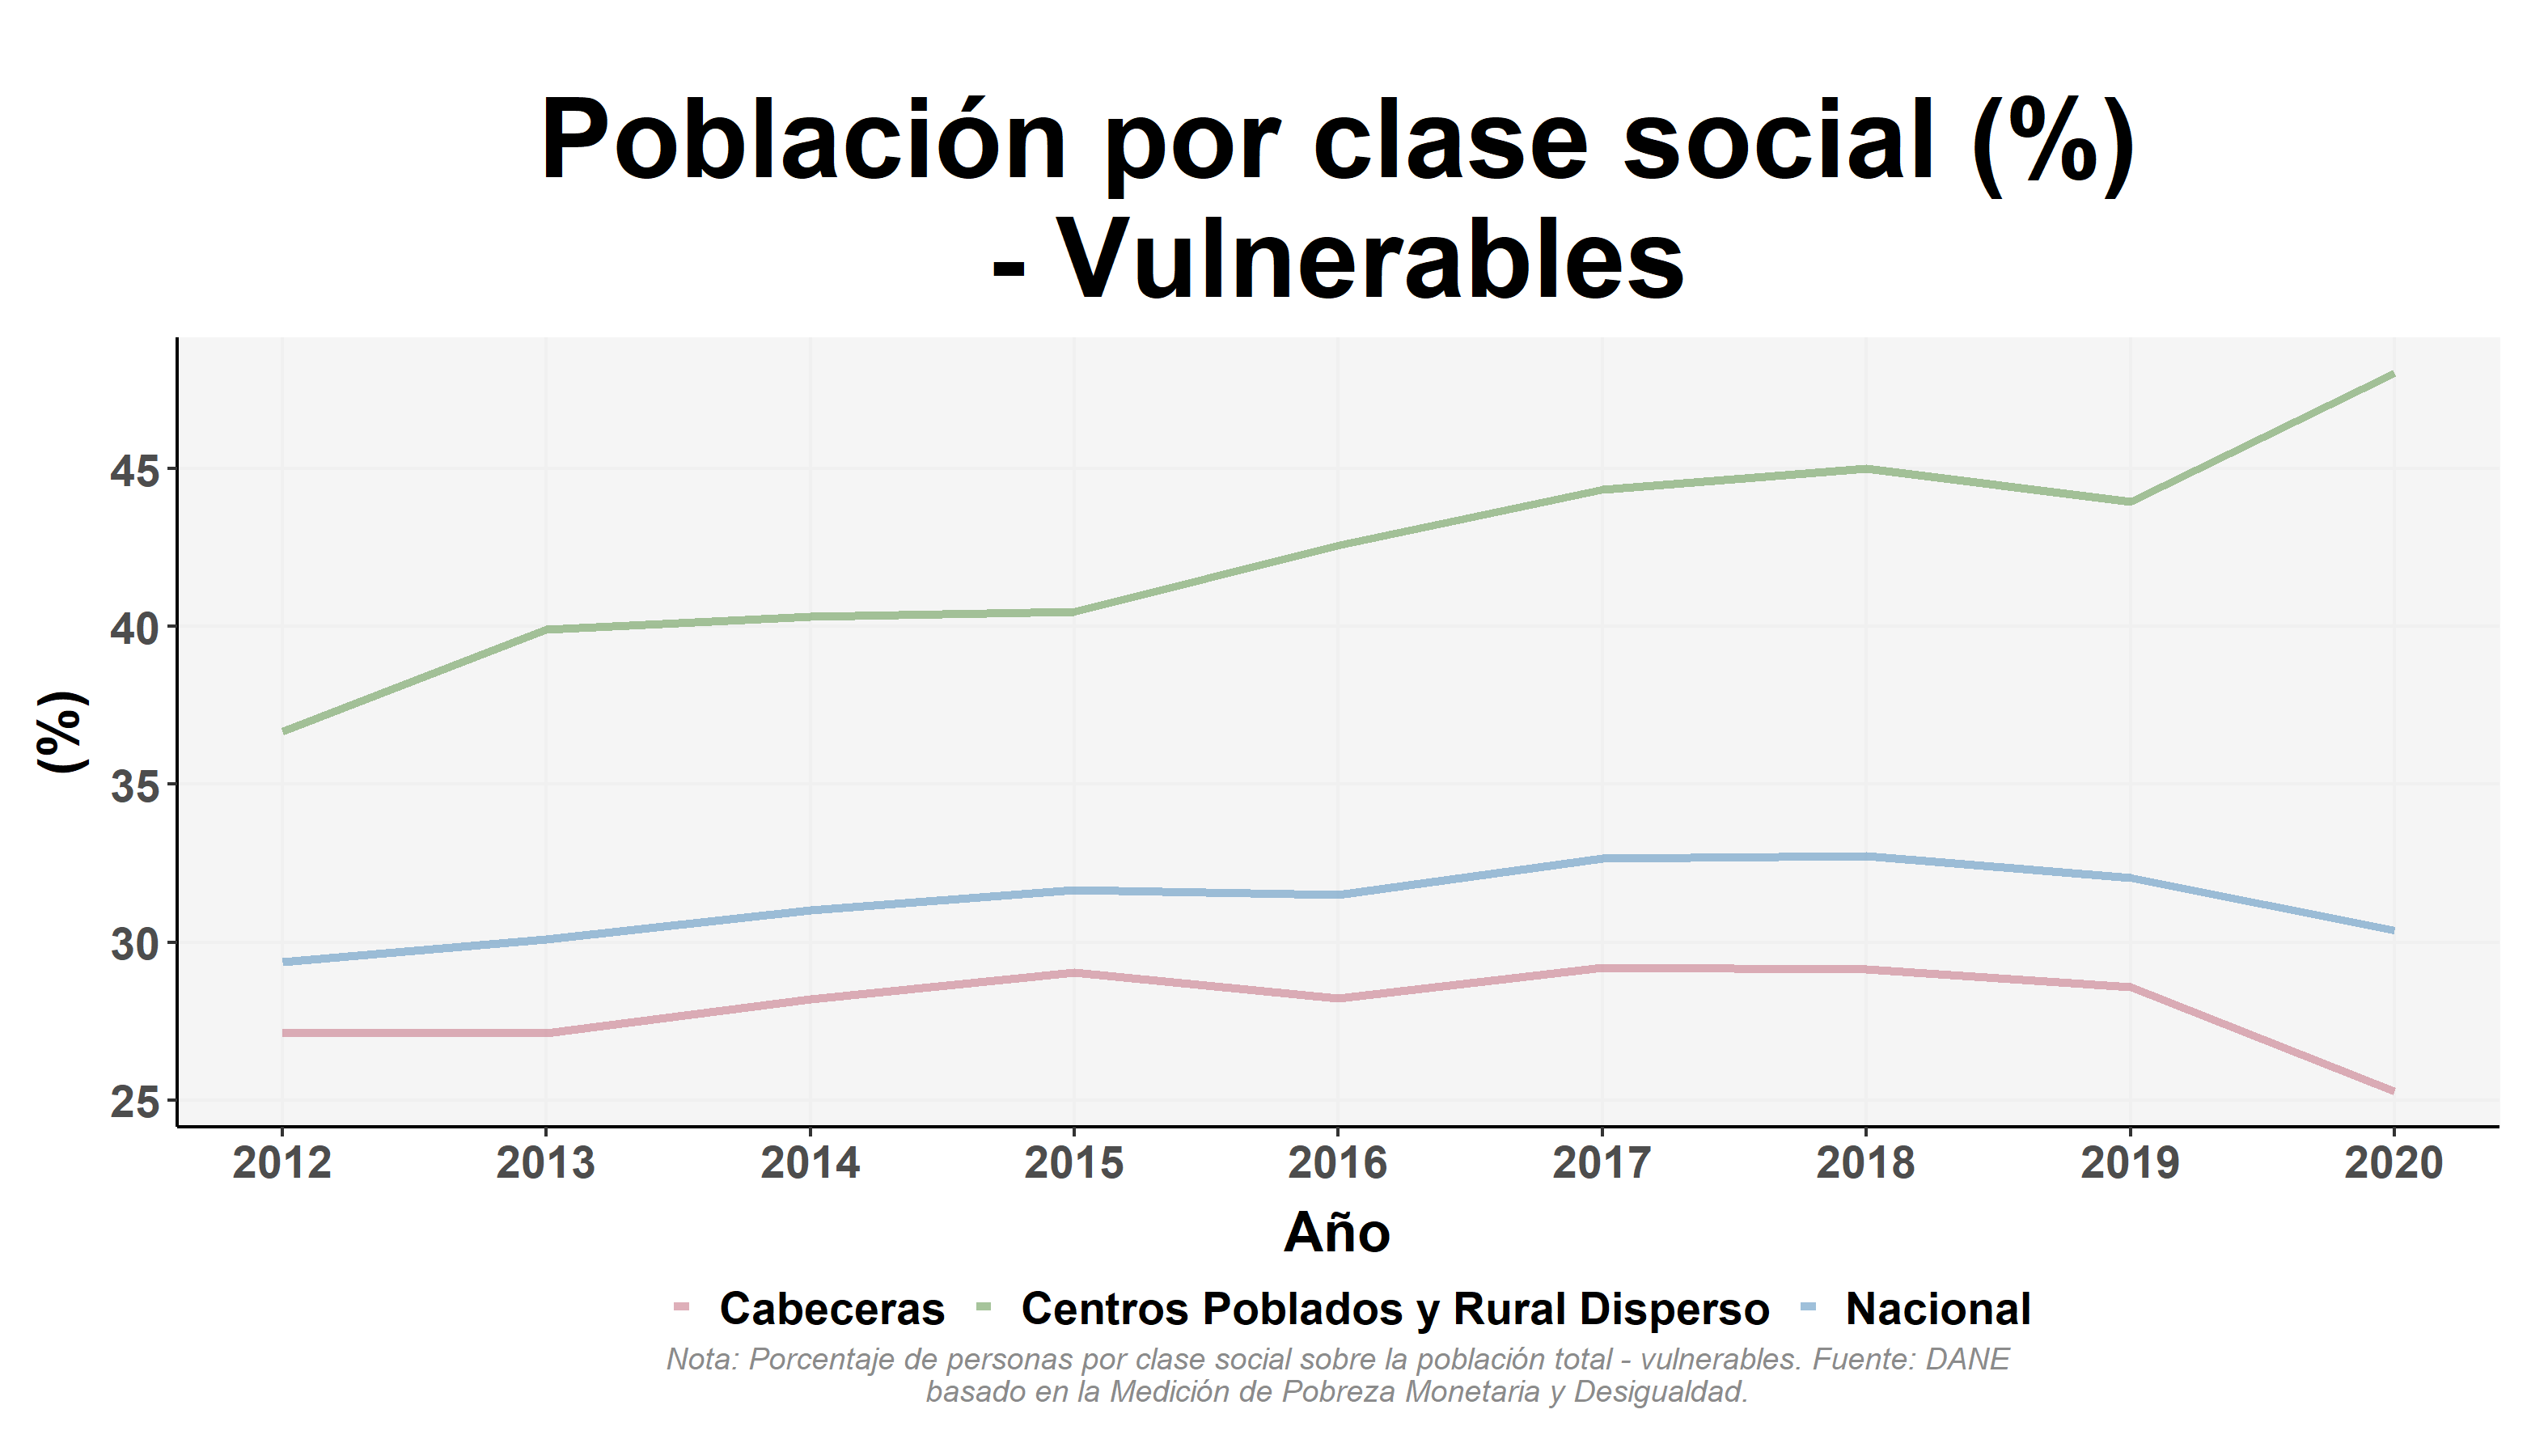
\includegraphics[width=\textwidth,keepaspectratio]{img/var_246_trend.png}
        \end{center}
    \end{figure}
            \begin{itemize}
                    \item En los centros poblados y rural disperso ha venido aumentando y fue el único que lo hizo para el 2020.
                    \item A nivel nacional y las cabeceras el porcentaje de vulnerables disminuyó desde el 2018 y se intensificó para el 2020.
                    \item Las cabeceras tienen niveles de vulnerables menores a los reportados en 2012, mientras que a nivel nacional son cercanos pero aun superiores.
                    \end{itemize}

%%%% Include figures
    \begin{figure}[H]
        \caption[Población por clase social - Clase media (2012 VS 2020) por ciudades ]{\label{clase_media_ciudades_vs} }
        \begin{center}
        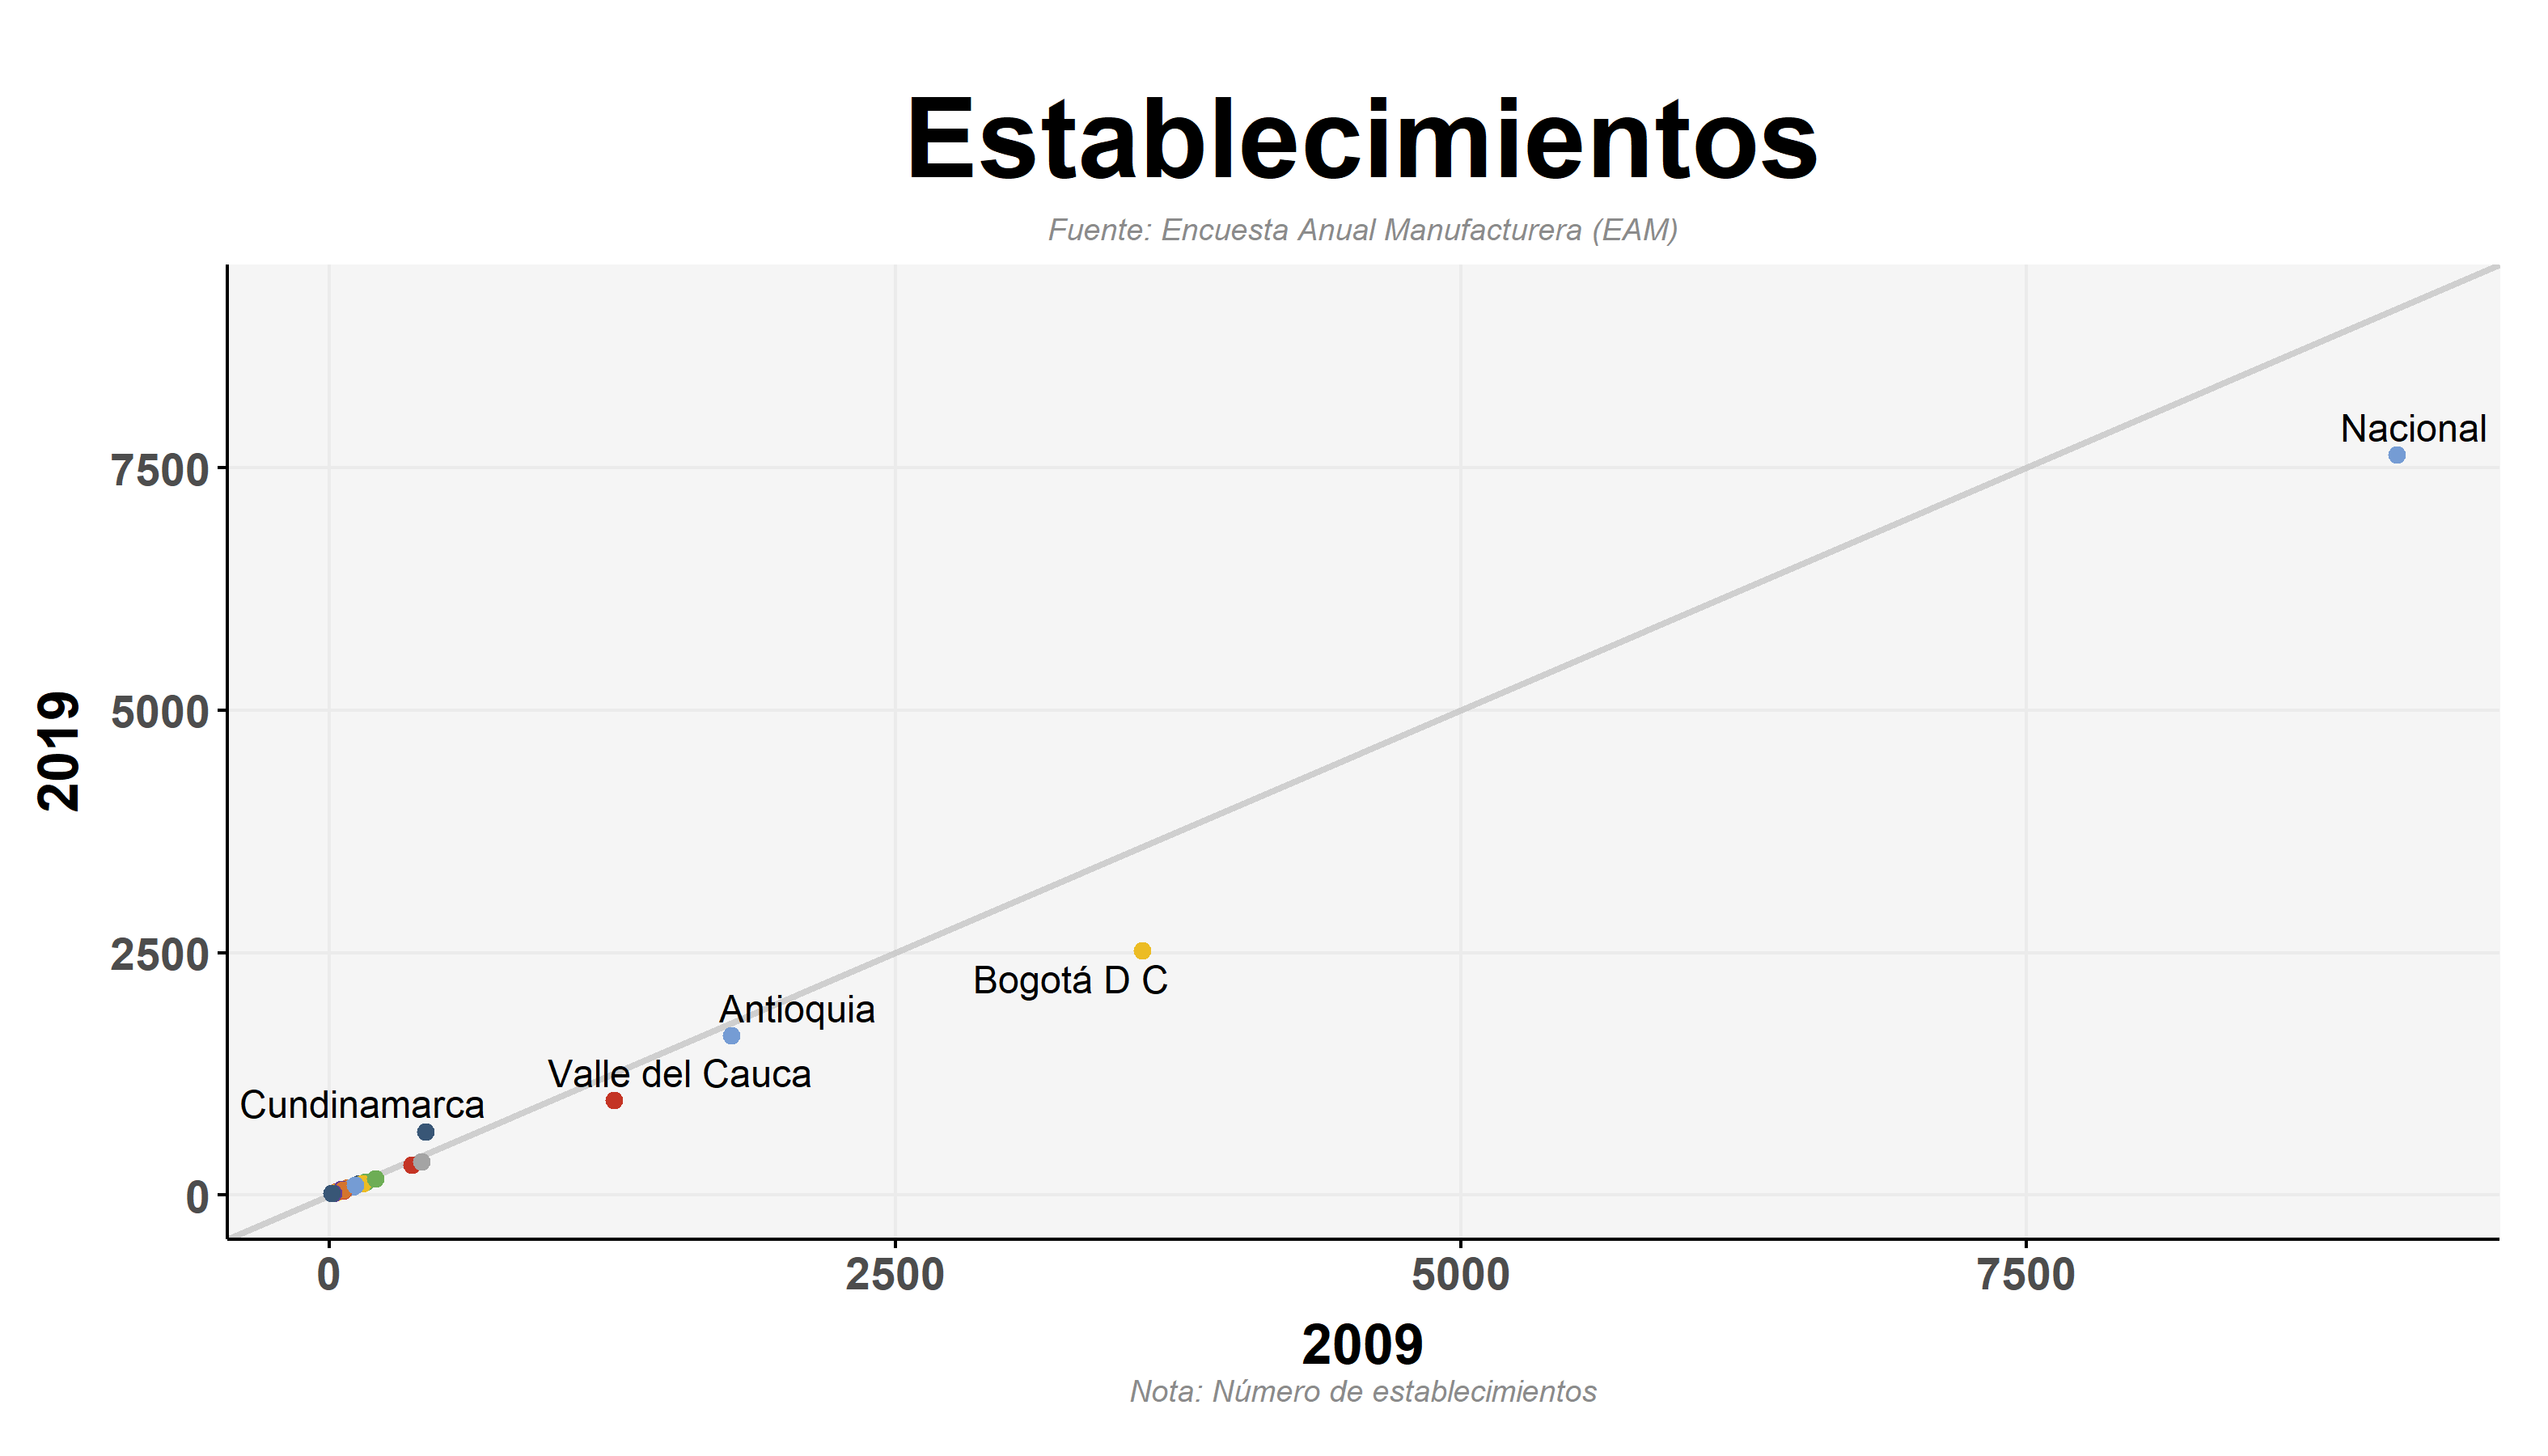
\includegraphics[width=\textwidth,keepaspectratio]{img/var_247_scatter_time.png}
        \end{center}
    \end{figure}
            \begin{itemize}
                    \item Pasto, Popayán y Quibdó mejoraron para 2020 el porcentaje de clase media con respecto a los registrados en 2012.
                    \item Florencia, Armenia y Cali registraron un porcentaje de clase social en 2020 iguales a los de 2012.
                    \item Las demás ciudades principales registraron niveles menores de población en clase media en 2020 comparado con los de 2012.
                    \item Para 2020 la diferencia entre las ciudades extremo es poco más del 25\% (Medellín - Riohacha).
                    \end{itemize}

%%%% Include figures
    \begin{figure}[H]
        \caption[Población por clase social - Clase media a nivel nacional ]{\label{clase_media_nacional} }
        \begin{center}
        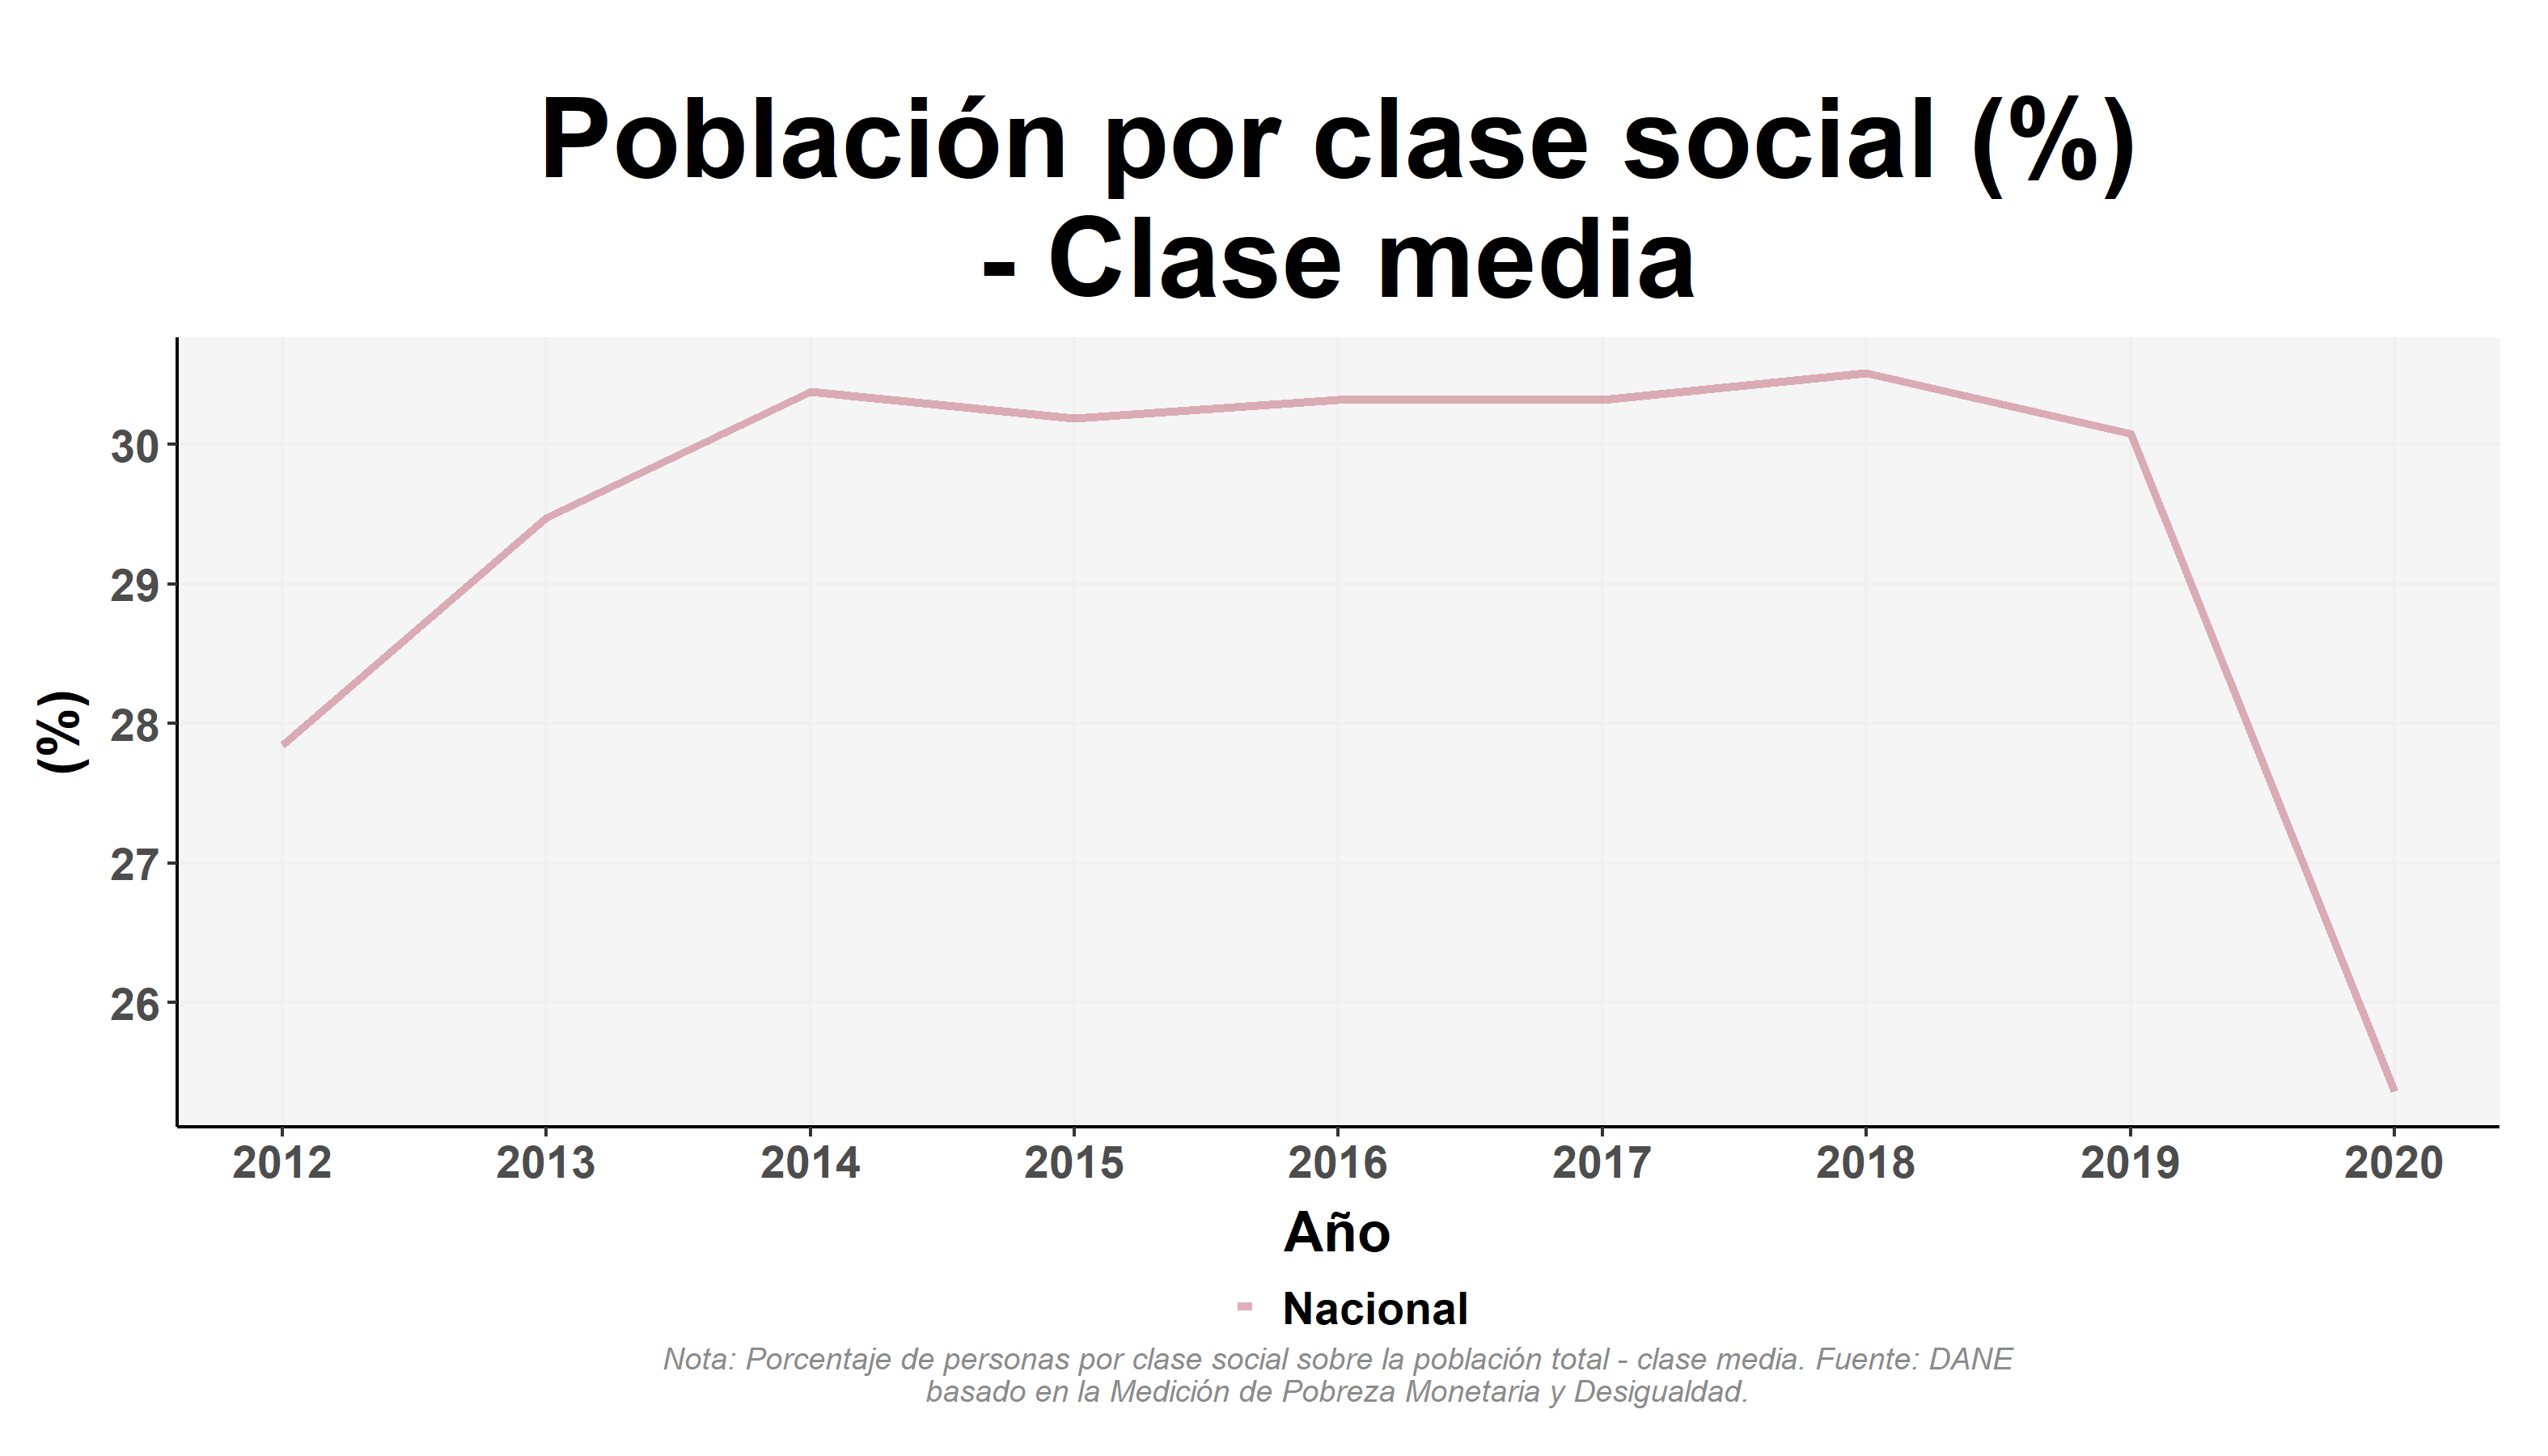
\includegraphics[width=\textwidth,keepaspectratio]{img/var_248_trend.png}
        \end{center}
    \end{figure}
            \begin{itemize}
                    \item El porcentaje de clase media a nivel nacional estuvo estancado después del 2014 hasta el 2018, donde empezó a disminuir.
                    \item A partir del 2018 empieza a decaer, lo cual se intensifica en el 2020.
                    \item El nivel de porcentaje de clase media para el 2020 está por debajo de los registrados en el 2012.
                    \item Desde el 2012 hasta el 2014 el porcentaje de personas de clase media estaba en aumento.
                    \end{itemize}

%%%% Include figures
    \begin{figure}[H]
        \caption[Población por clase social - Clase media por zonas ]{\label{clase_media_zonas} }
        \begin{center}
        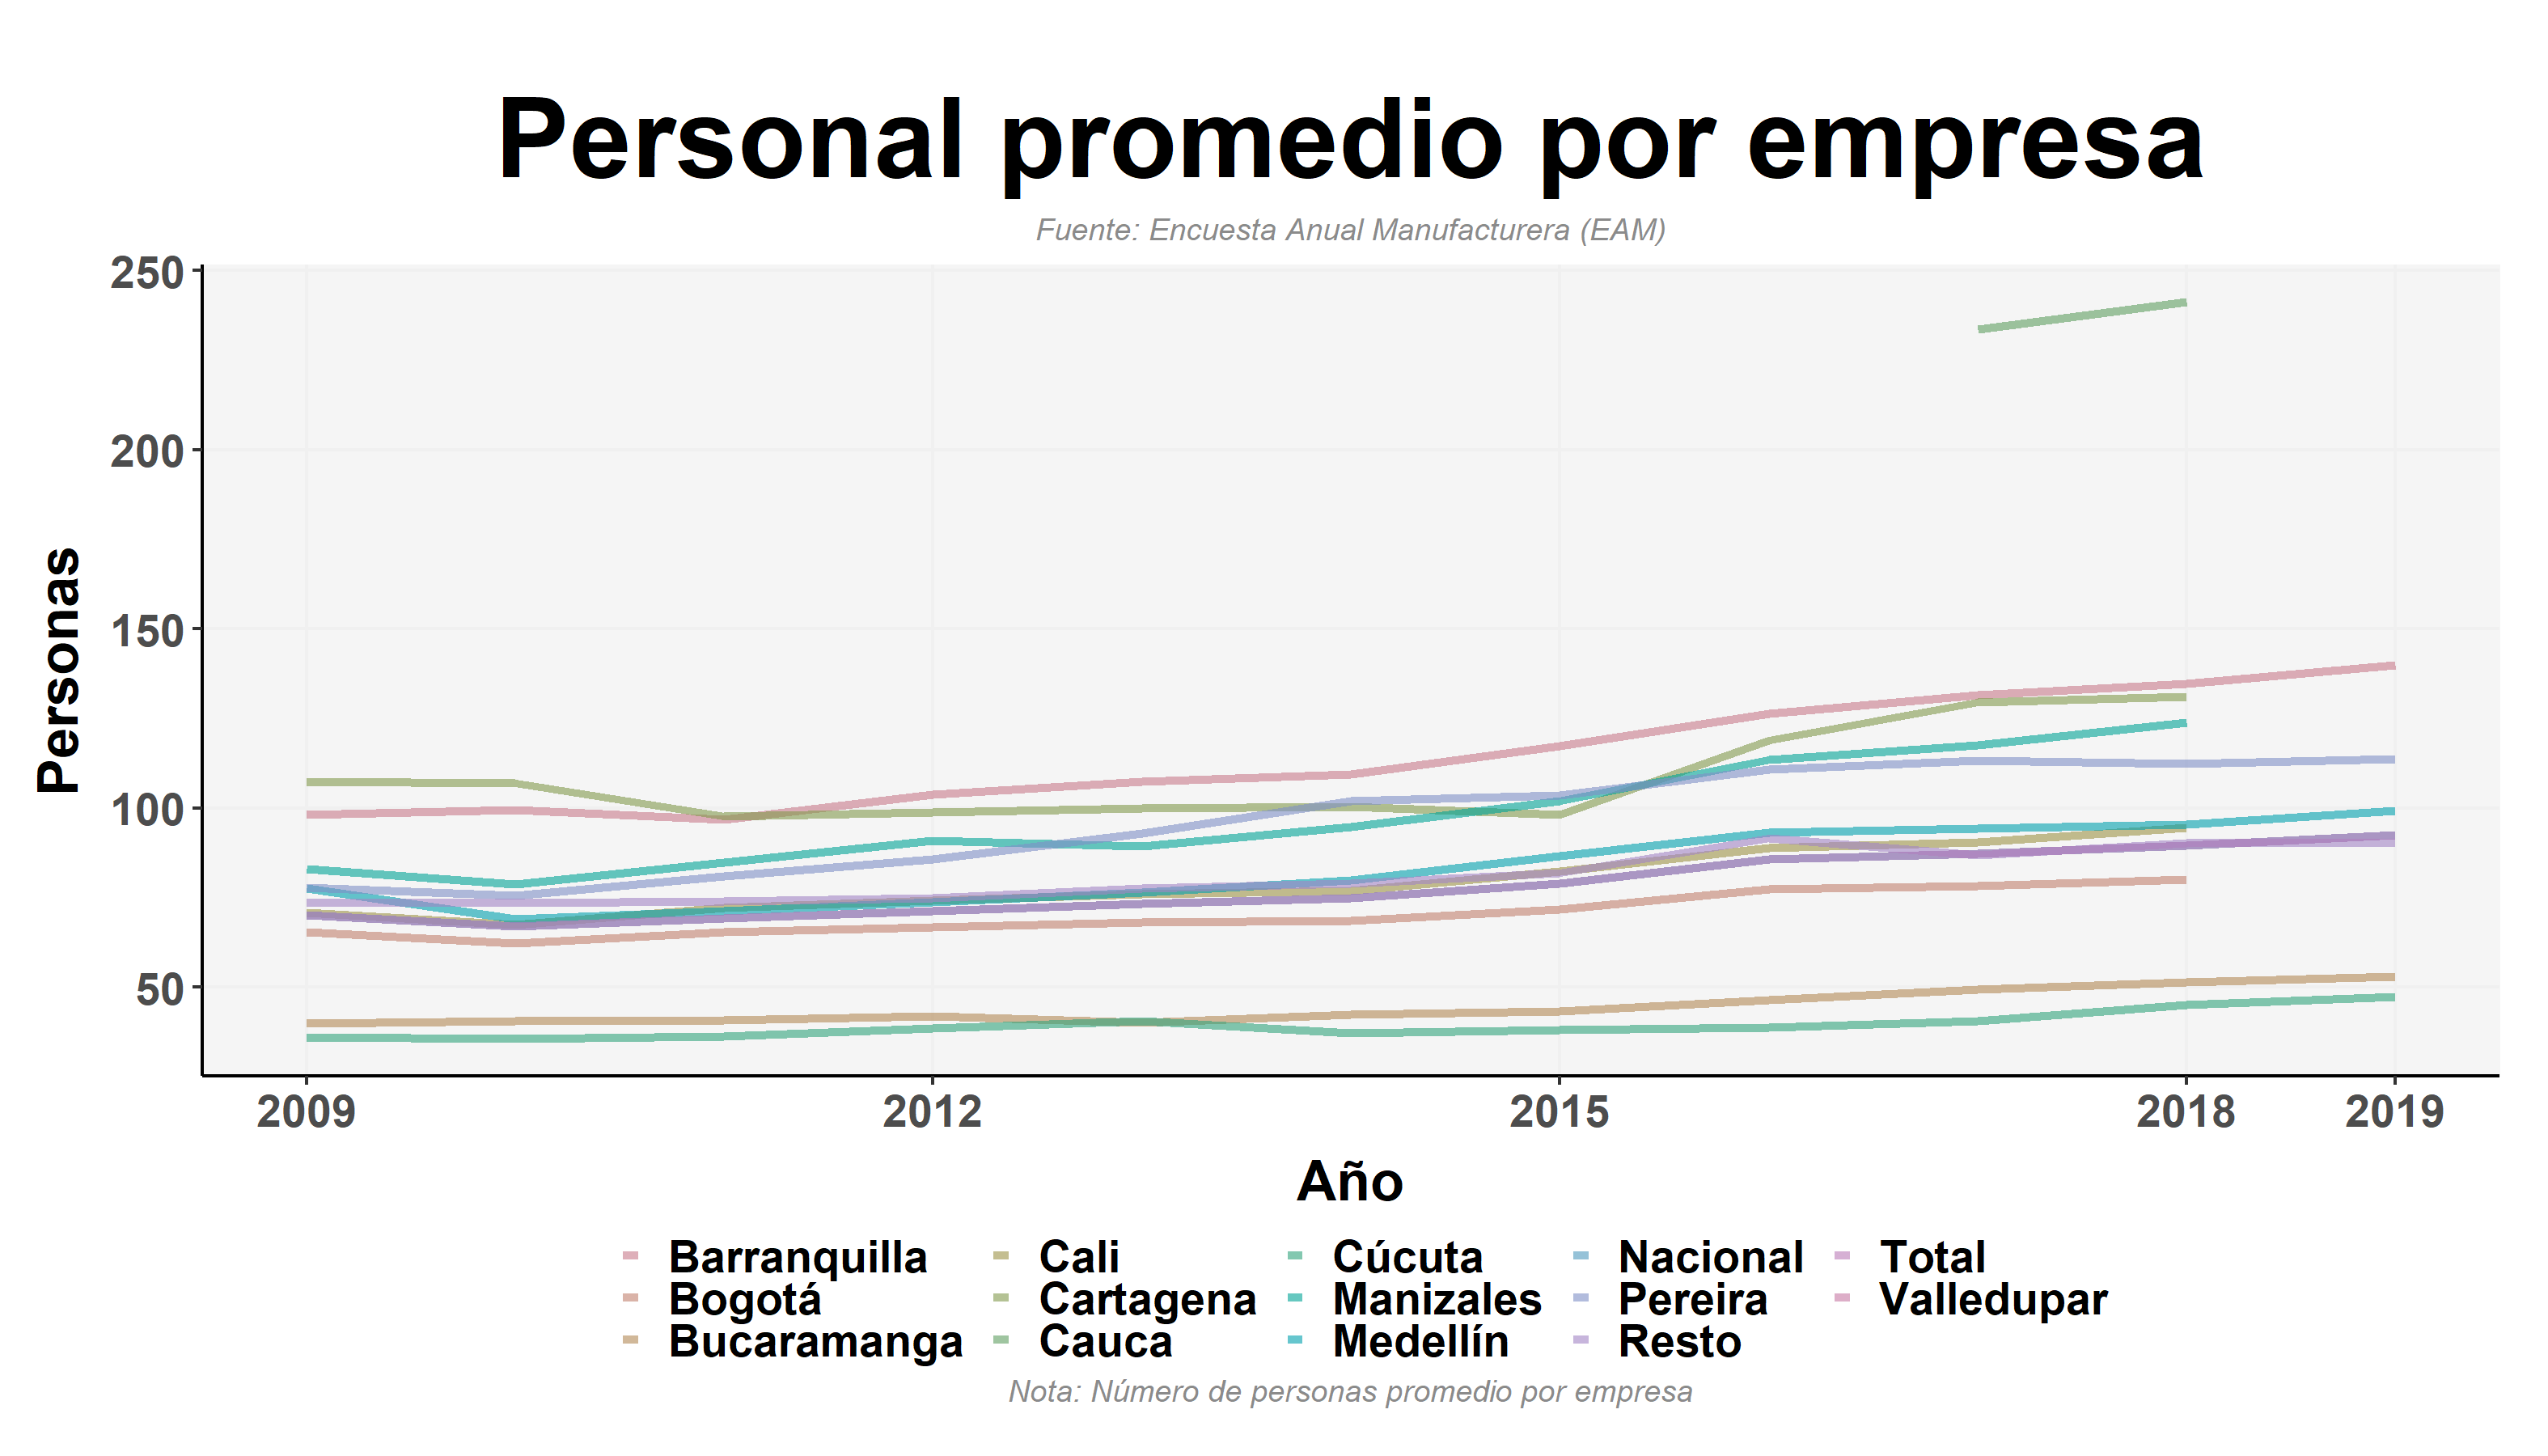
\includegraphics[width=\textwidth,keepaspectratio]{img/var_249_trend.png}
        \end{center}
    \end{figure}
            \begin{itemize}
                    \item Para los centros poblados y rural disperso los niveles de personas de clase media han tenido un leve aumento hasta el 2017 donde inicio a decaer pero se recuperó para el 2020.
                    \item A nivel nacional y cabeceras los niveles de clase media han estado constantes hasta el 2019, en el 2020 presenta una caída abrupta.
                    \item Para 2020 los niveles registrados de clase media a nivel nacional y cabeceras son menores a los registrados en el 2012.
                    \end{itemize}

%%%% Include figures
    \begin{figure}[H]
        \caption[Población por clase social - Clase alta (2012 VS 2020) por ciudad ]{\label{clase_alta_ciudades_vs} }
        \begin{center}
        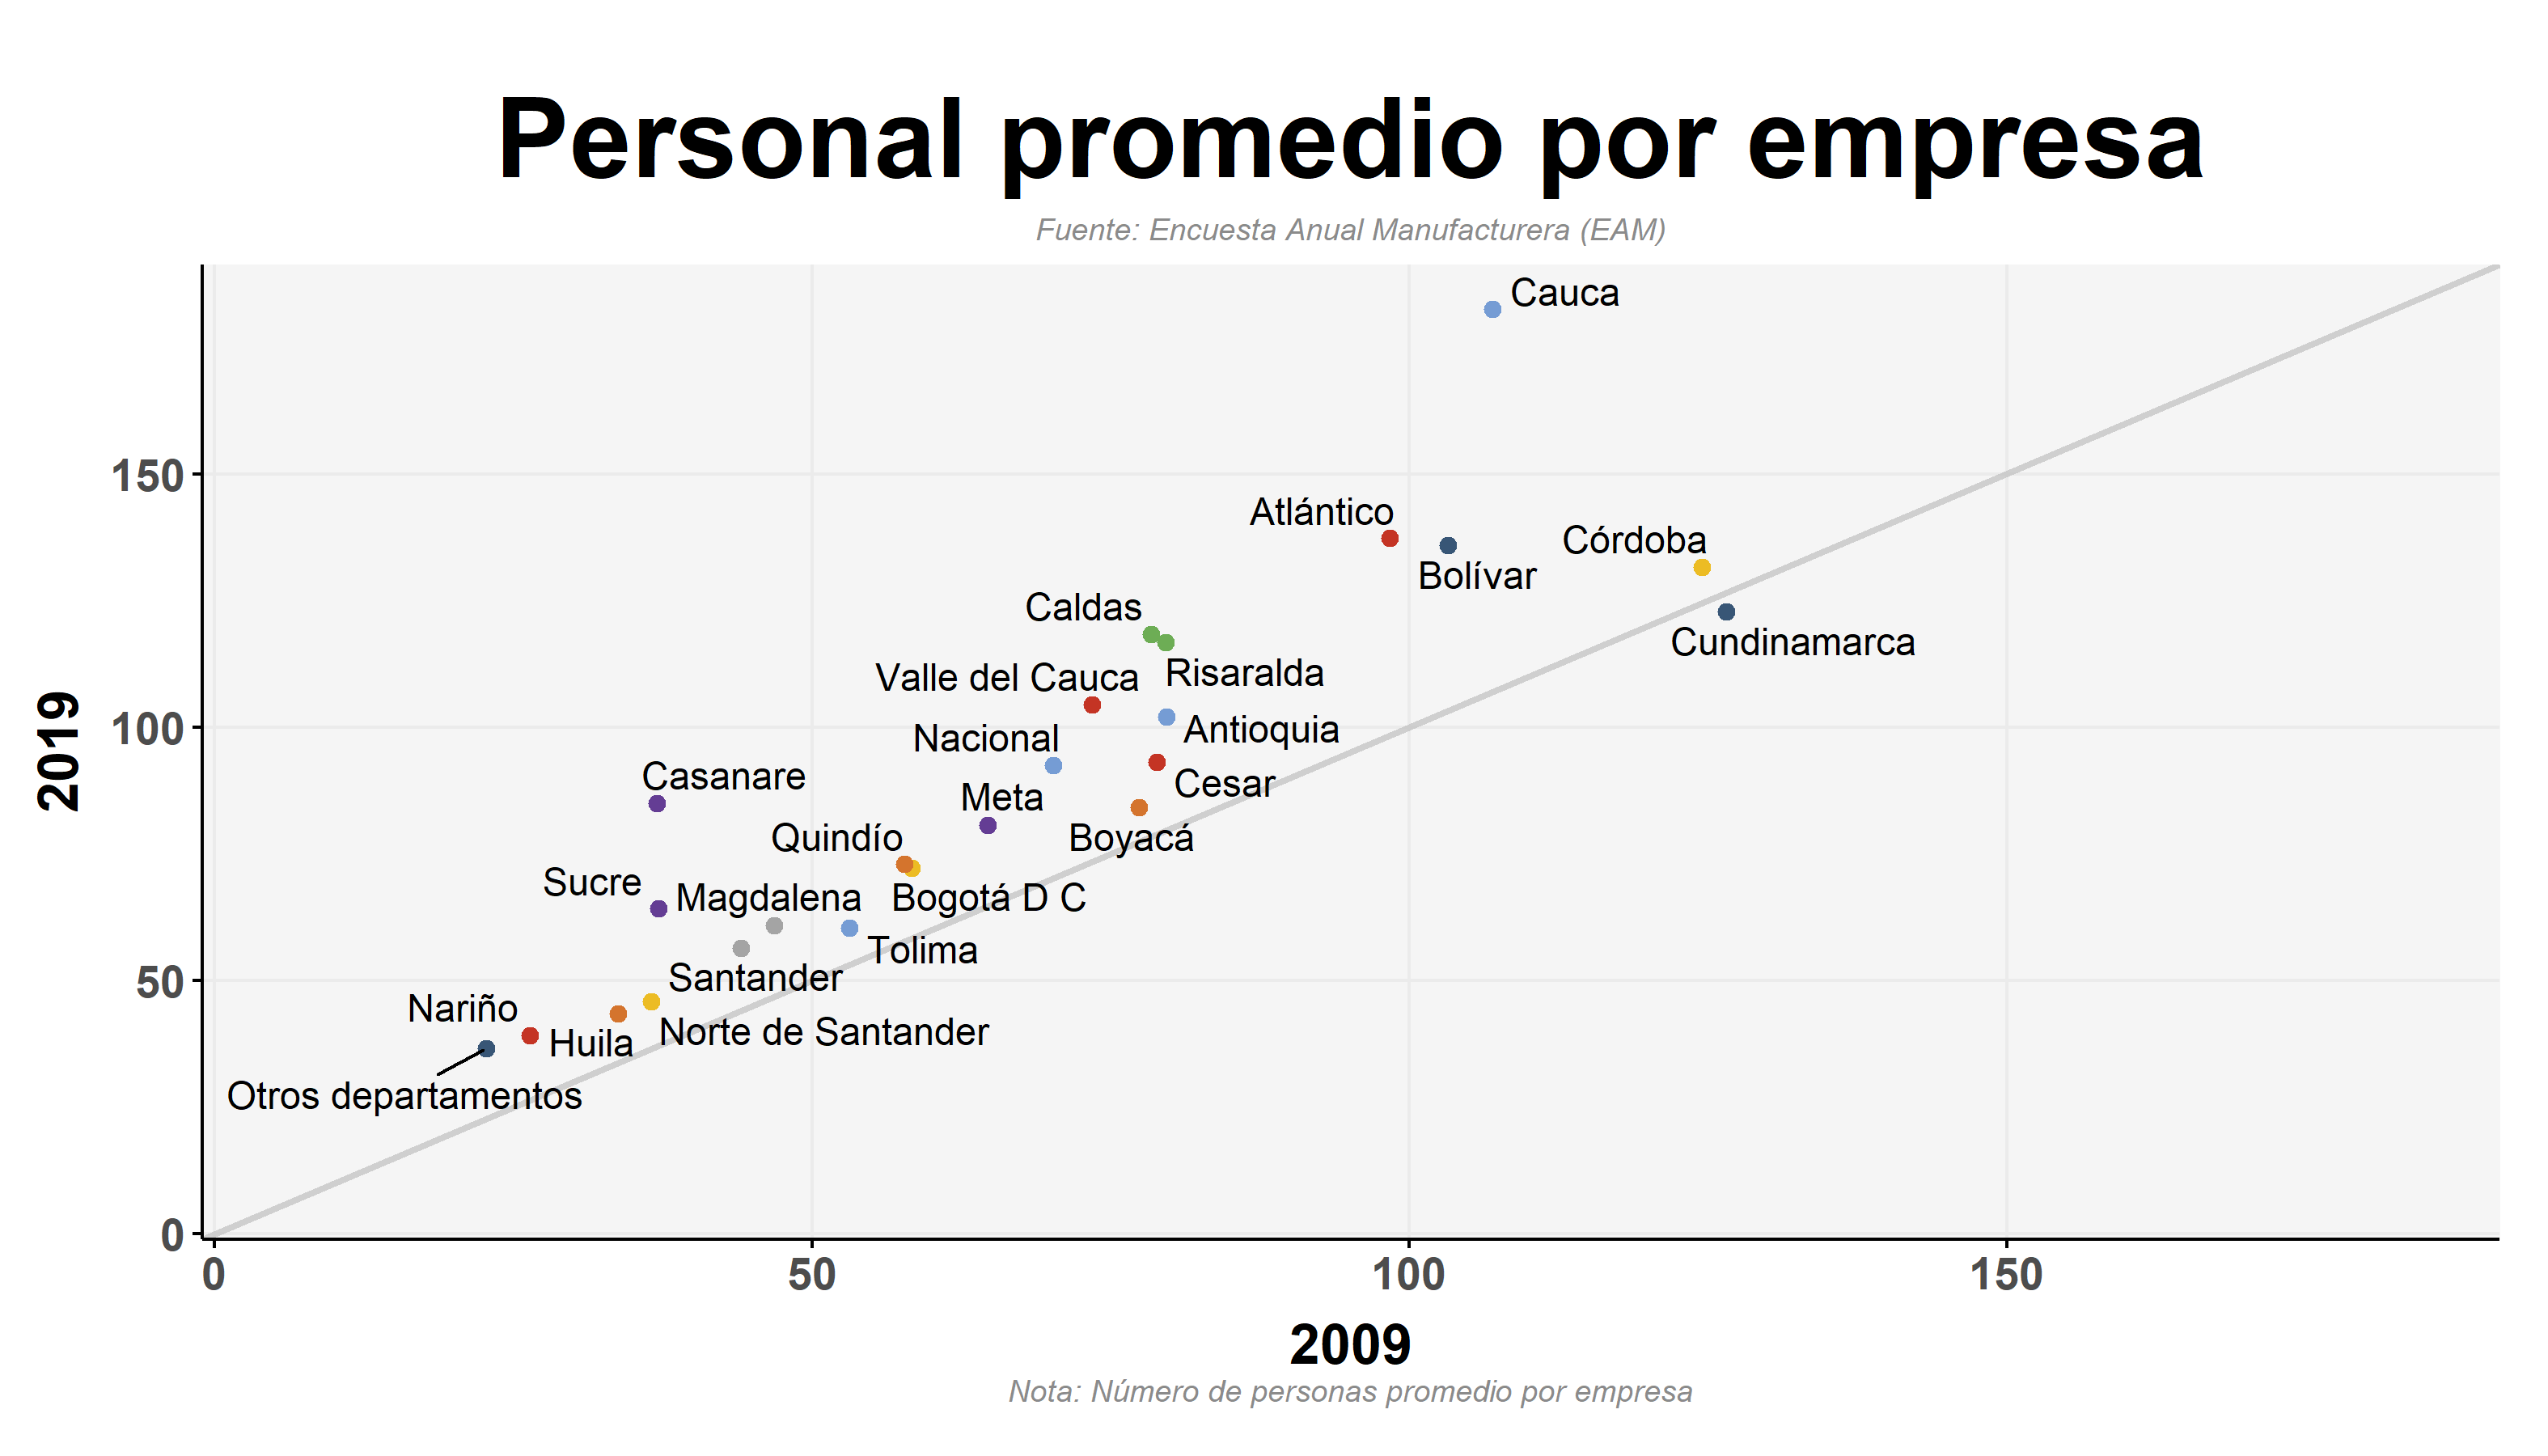
\includegraphics[width=\textwidth,keepaspectratio]{img/var_250_scatter_time.png}
        \end{center}
    \end{figure}
            \begin{itemize}
                    \item Pasto es la única ciudad que presenta mejores niveles de clase alta en el 2020, comparado con los de 2012.
                    \item Cúcuta y Barranquilla presentan niveles de clase alta similares entre 2012 y 2020.
                    \item Medellín y Bogotá son las ciudades con más alto nivel de población de clase alta estando alejadas de las otras ciudades.
                    \item Hay una diferencia de 4\% entre las ciudades extremo (Medellín - Riohacha).
                    \item Ninguna ciudad presenta una población de clase alta por encima del 5\%, gran parte de las ciudades está por debajo del 3\%.
                    \end{itemize}

%%%% Include figures
    \begin{figure}[H]
        \caption[Población por clase social - Clase alta a nivel nacional ]{\label{clase_alta_nacional} }
        \begin{center}
        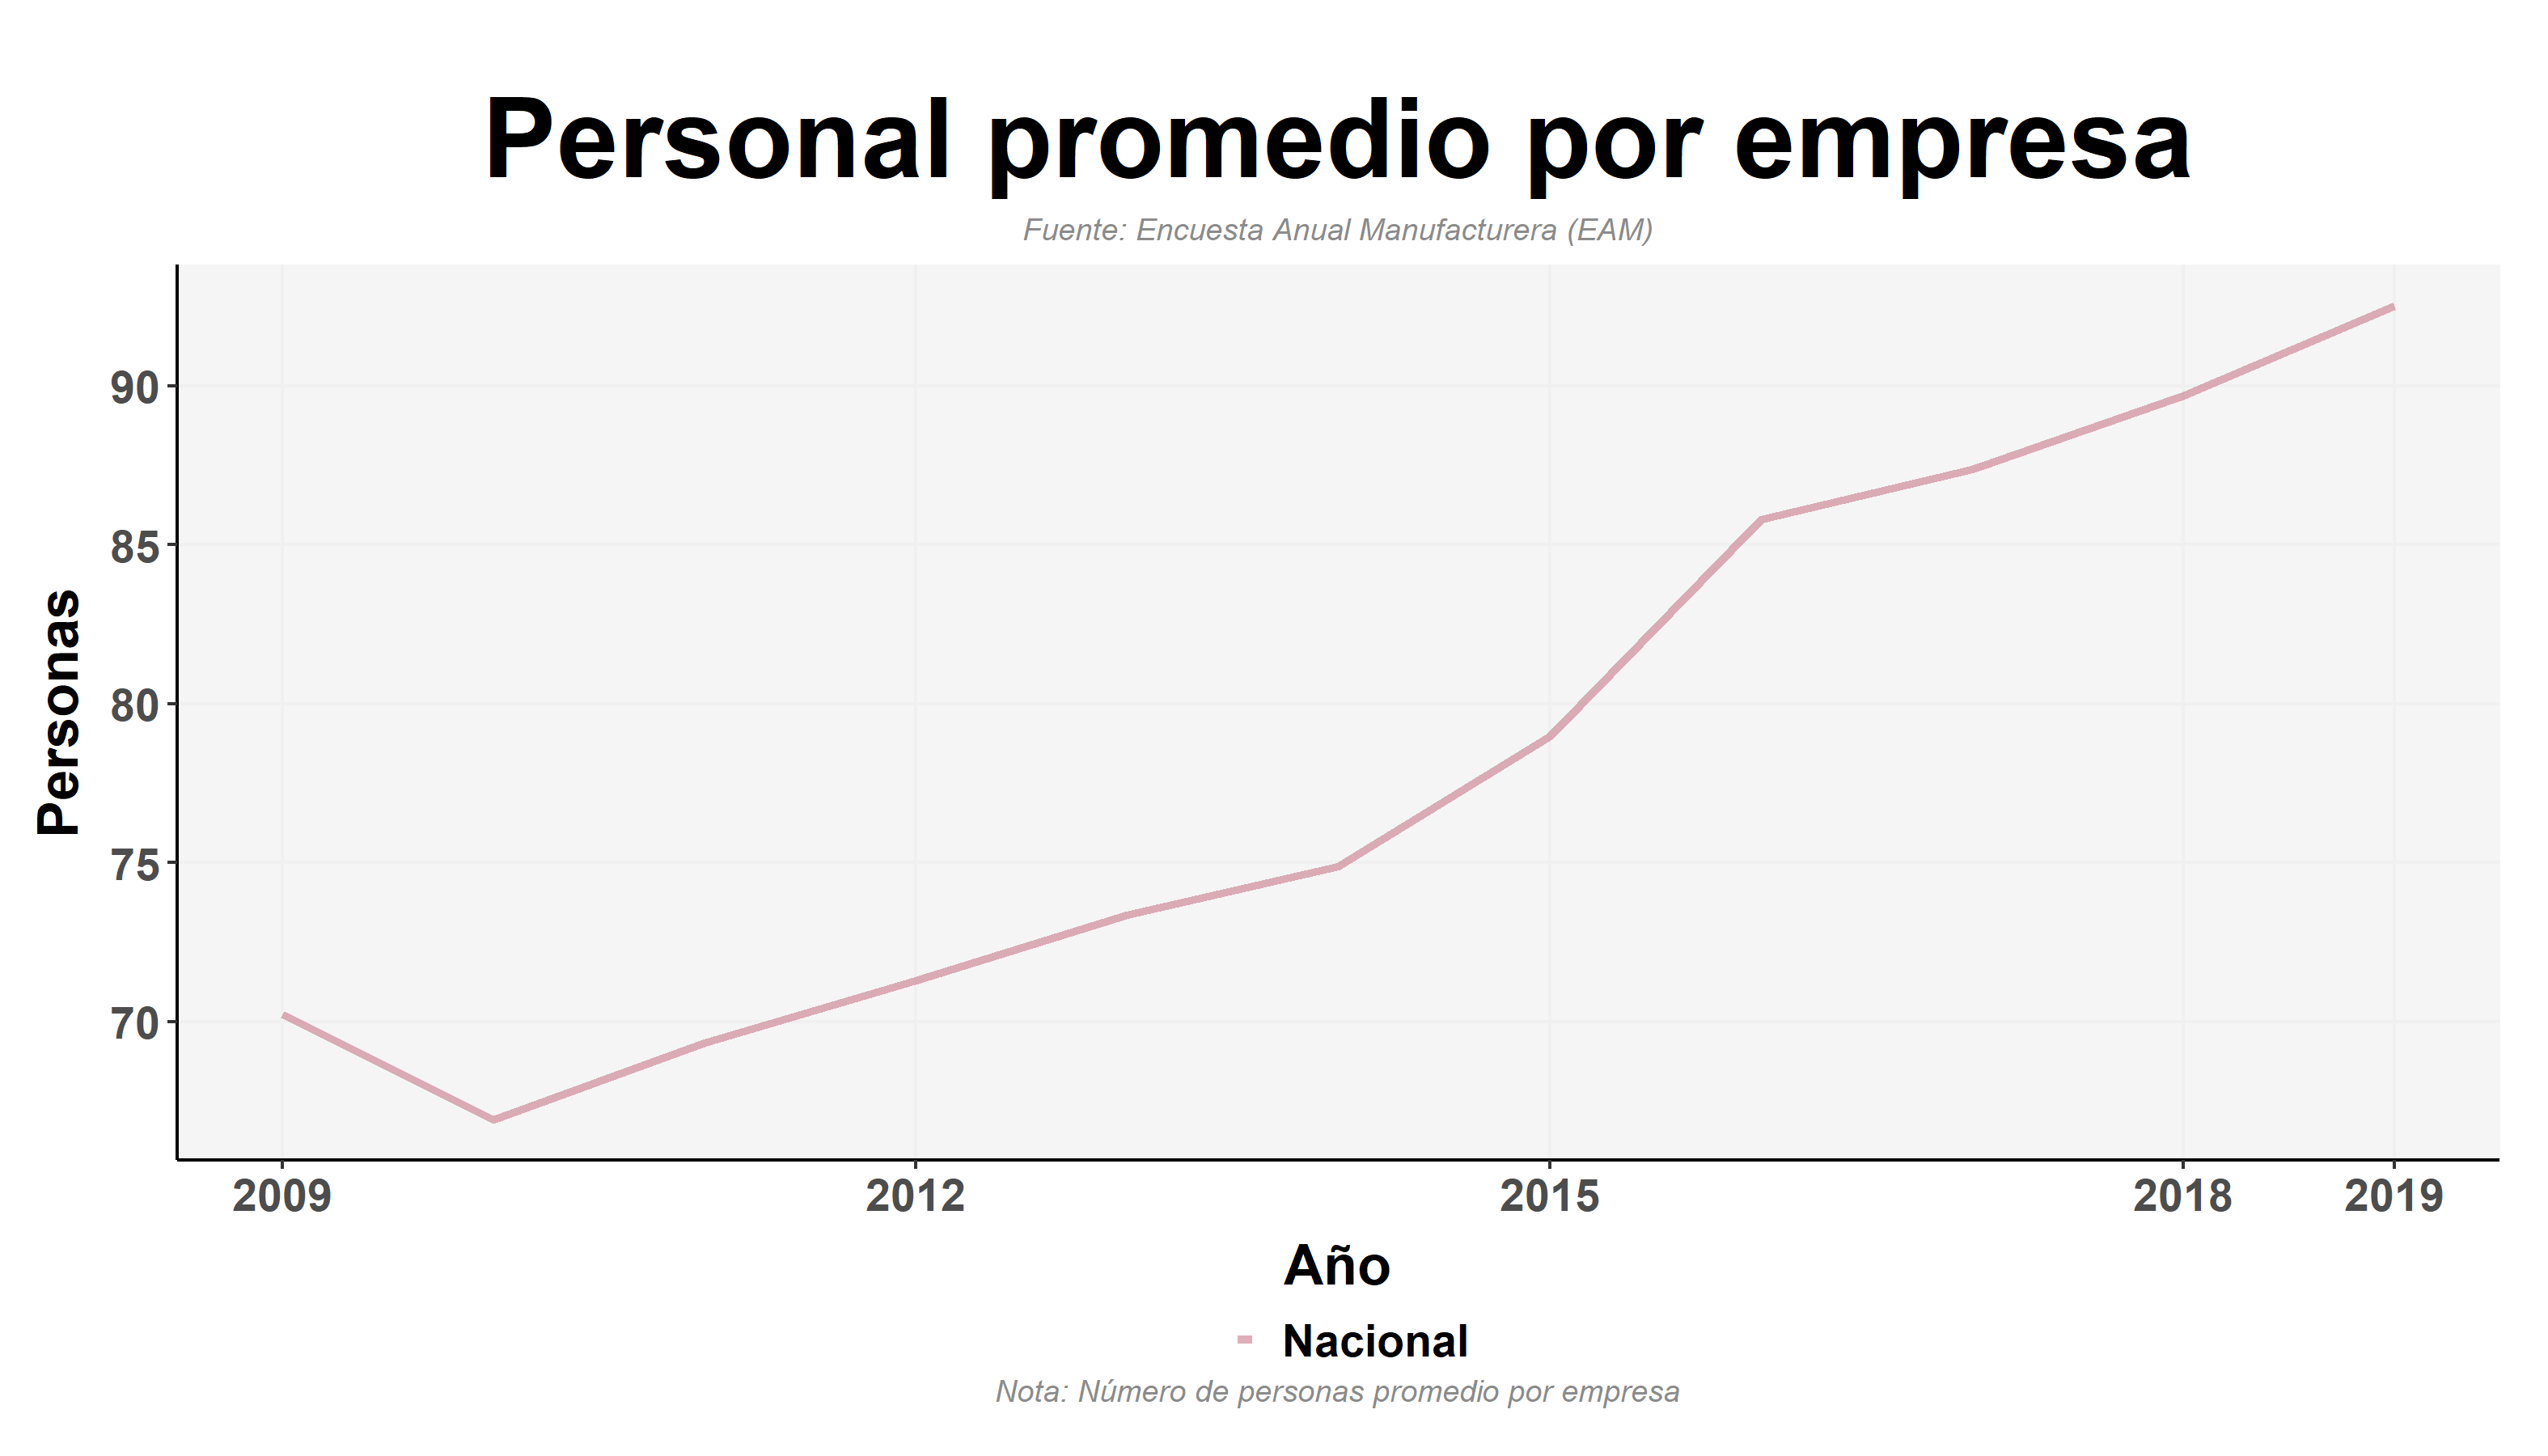
\includegraphics[width=\textwidth,keepaspectratio]{img/var_251_trend.png}
        \end{center}
    \end{figure}
            \begin{itemize}
                    \item La clase alta es la que demuestra mayor variación entre los años para el nivel nacional.
                    \item La clase alta presentó un decrecimiento después de 2014 hasta el 2017, repitiéndose en el 2020 donde cae abruptamente.
                    \item Para 2020 se registraron niveles menores comparado con los del 2012.
                    \end{itemize}

%%%% Include figures
    \begin{figure}[H]
        \caption[Población por clase social - Clase alta por zonas ]{\label{clase_alta_zonas} }
        \begin{center}
        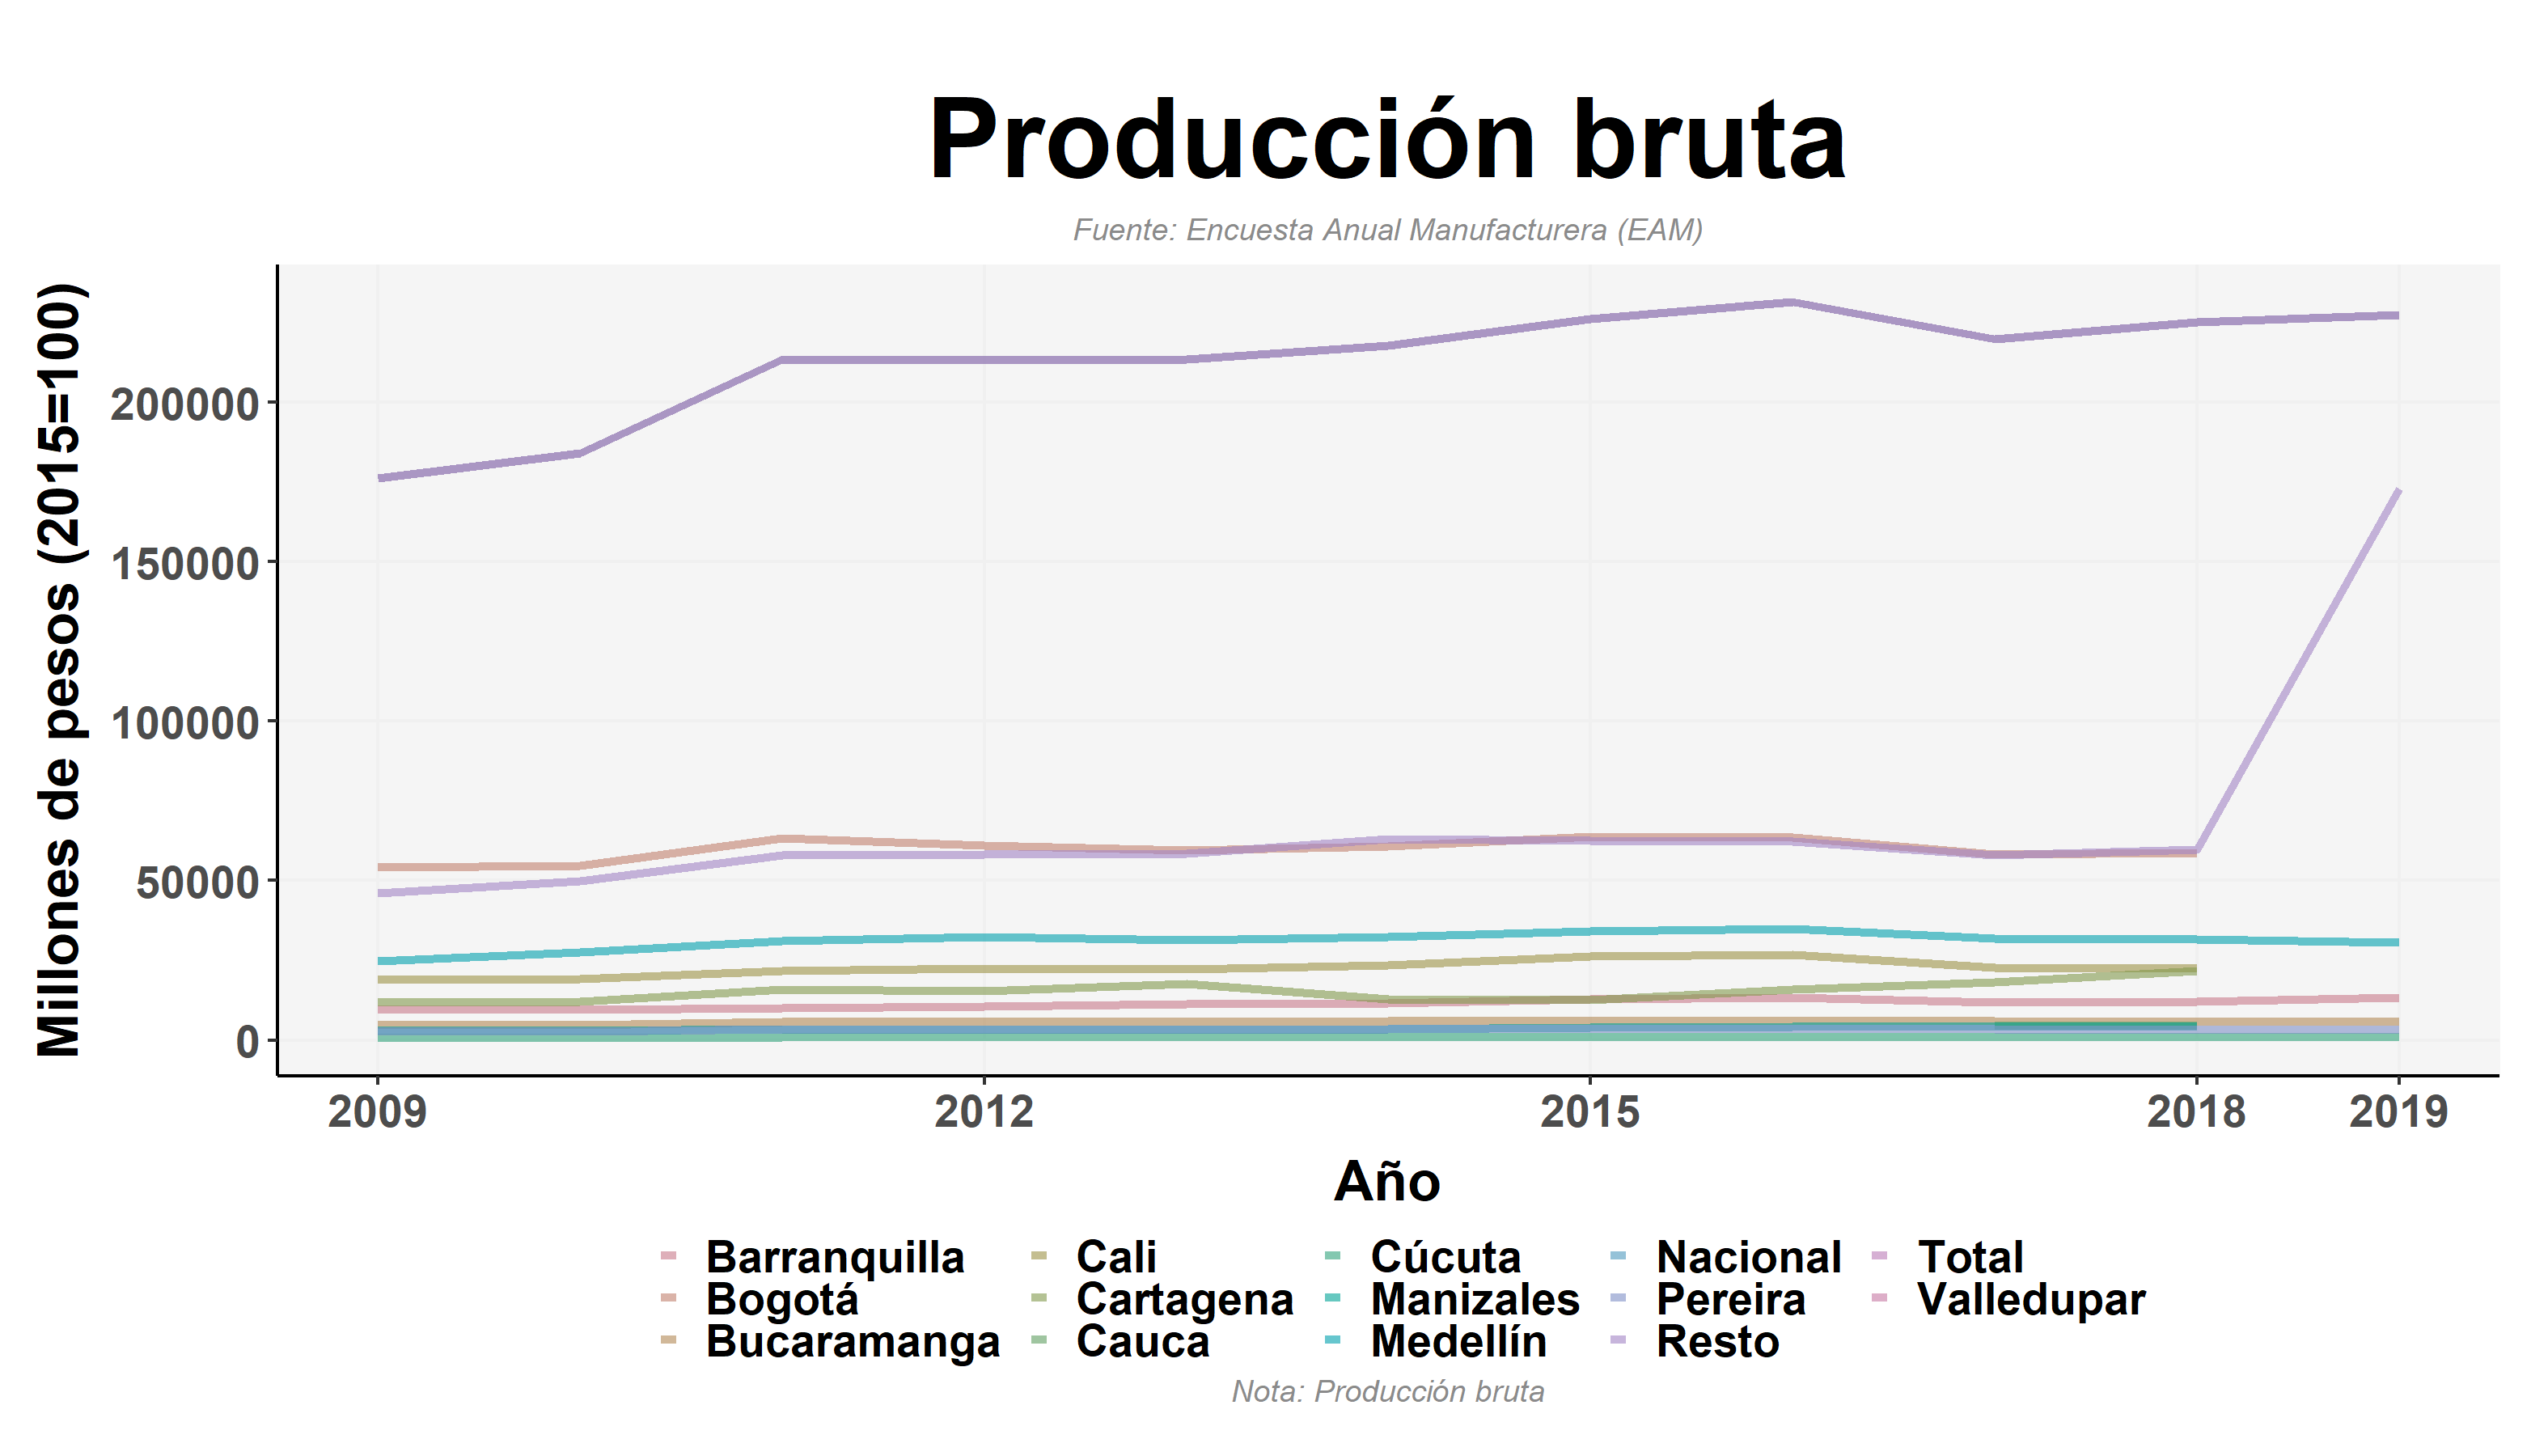
\includegraphics[width=\textwidth,keepaspectratio]{img/var_252_trend.png}
        \end{center}
    \end{figure}
            \begin{itemize}
                    \item Los centros poblados y el rural disperso presentan un crecimiento de la clase alta a lo largo del tiempo pero está por debajo del 1\% de la población.
                    \item Las cabeceras y a nivel nacional se presenta la misma tendencia, presentando para el 2020 niveles menores a los registrados en el 2012.
                    \end{itemize}

        \subsubsection{Pobreza Extrema}

%%%% Include figures
    \begin{figure}[H]
        \caption[Pobreza extrema por ciudades - 2012 VS 2020 ]{\label{pobreza_extrema_ciudades_vs} }
        \begin{center}
        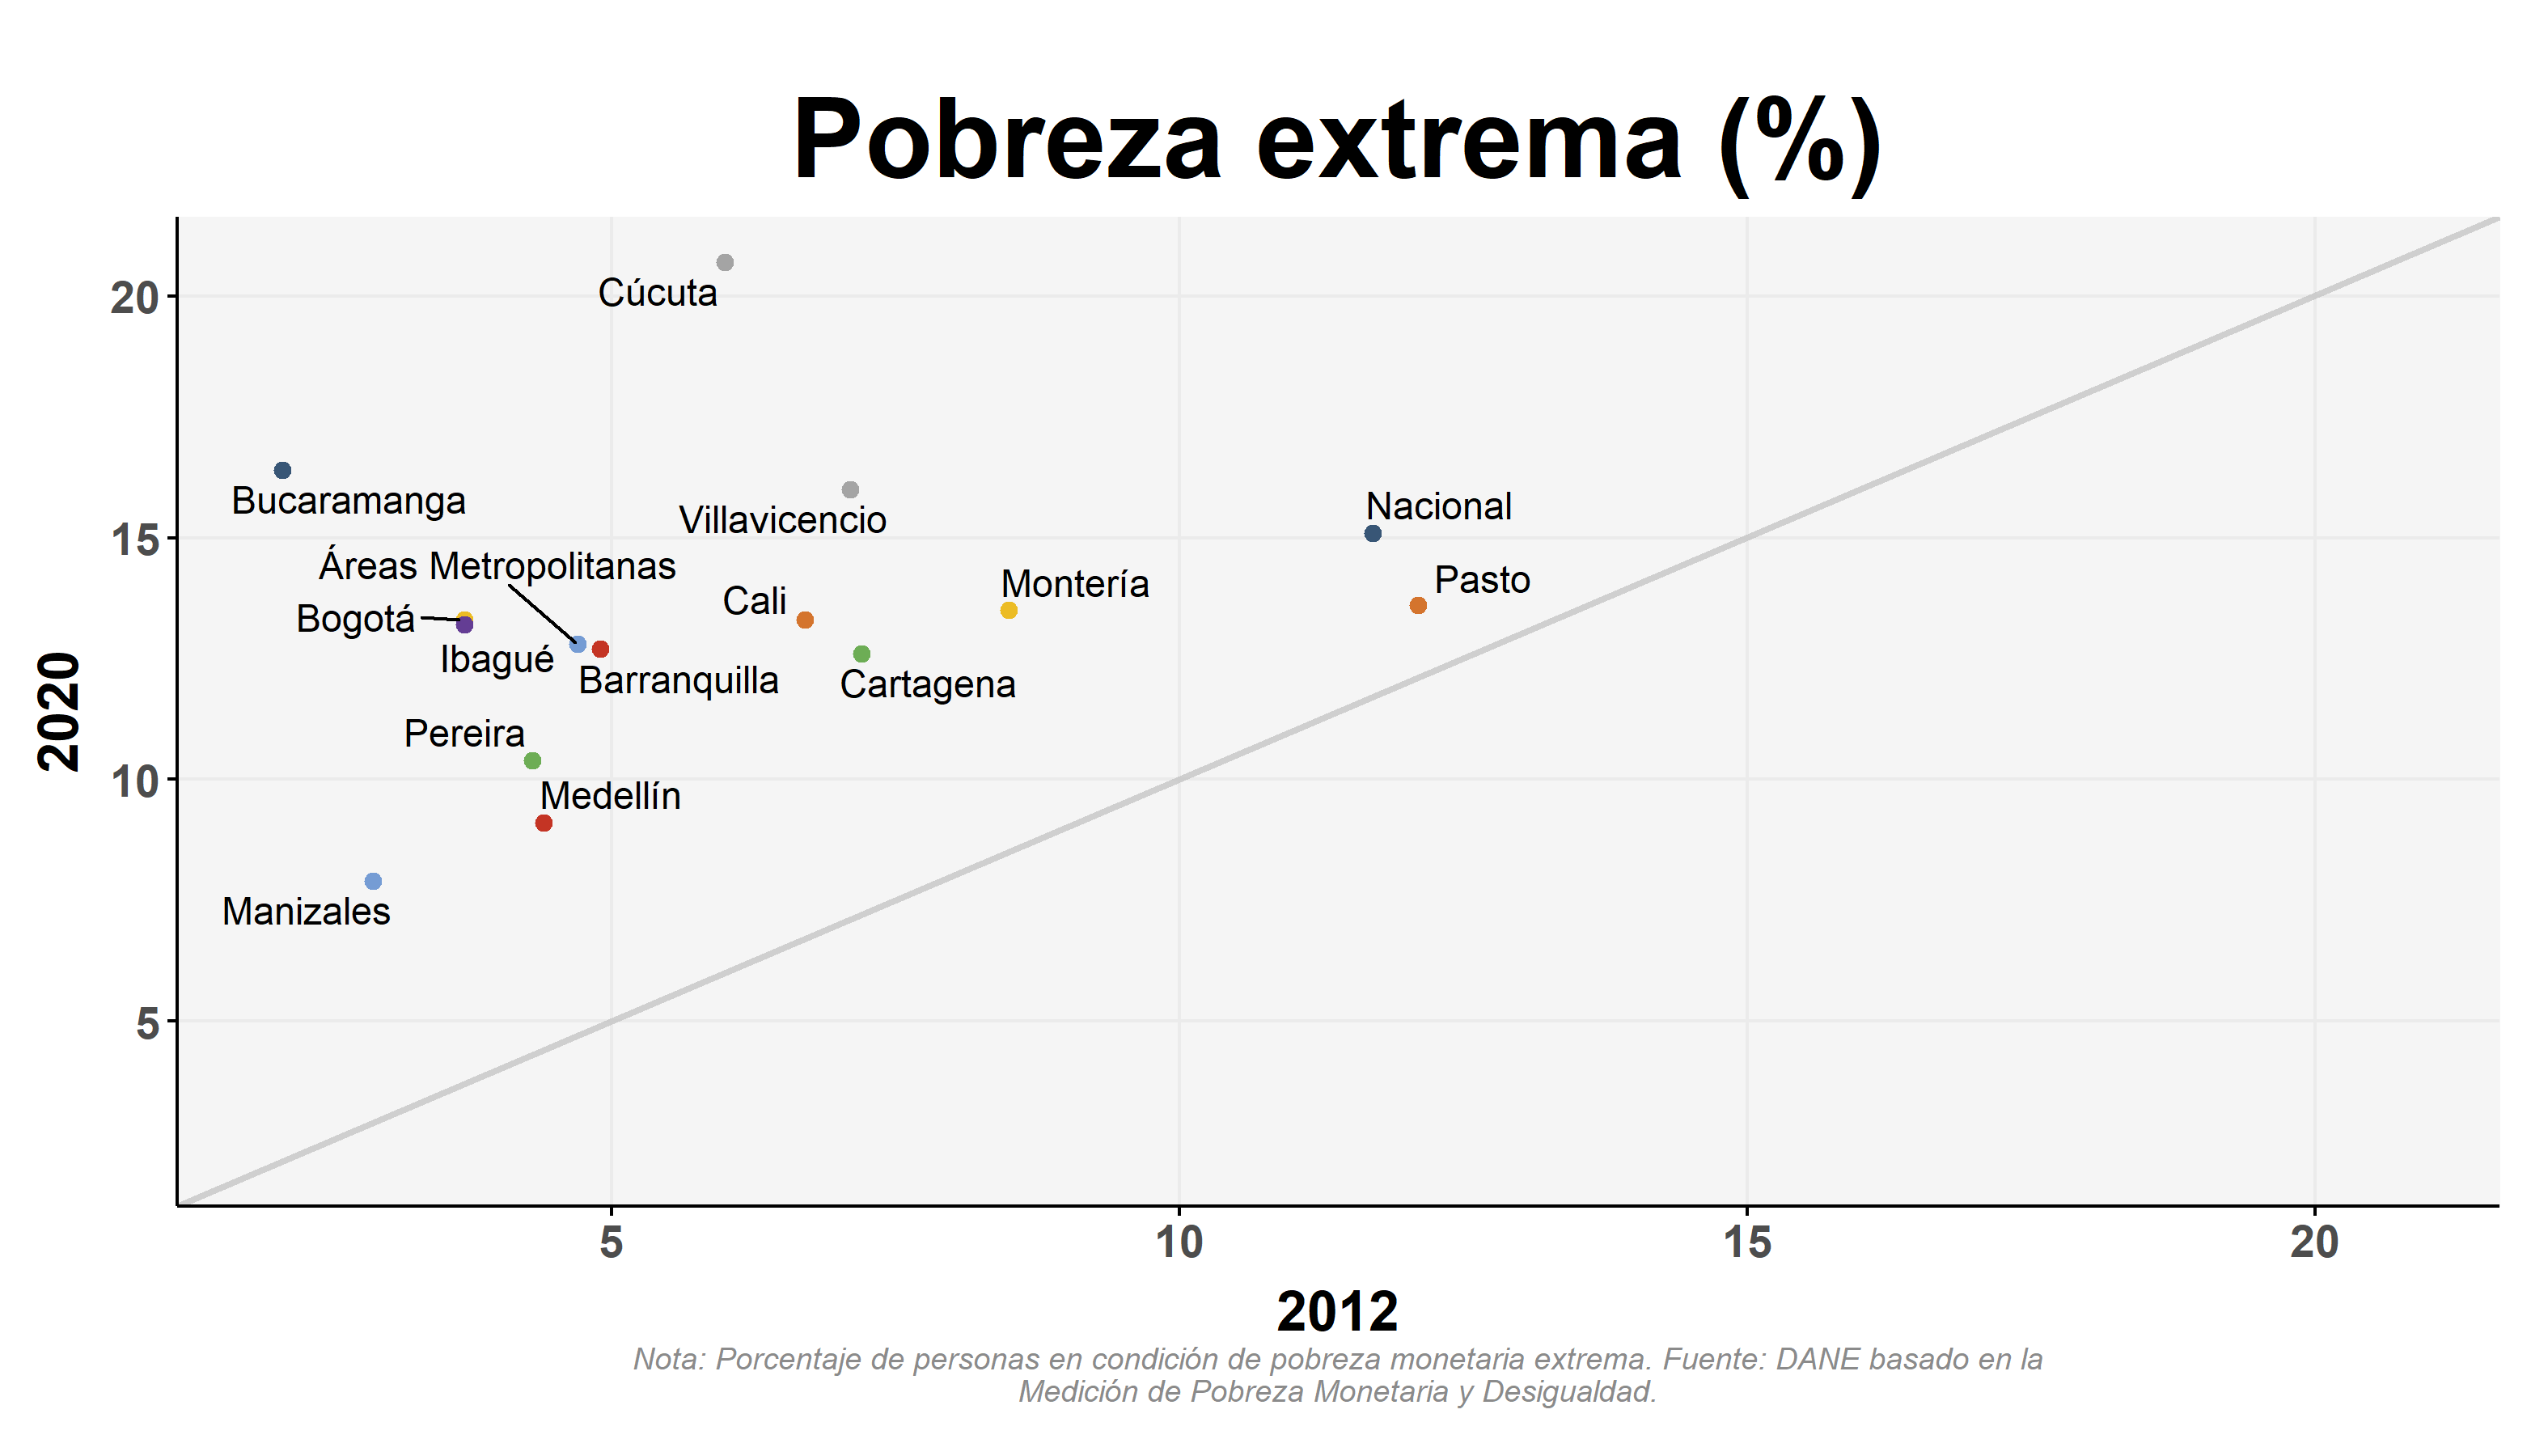
\includegraphics[width=\textwidth,keepaspectratio]{img/var_257_scatter_time.png}
        \end{center}
    \end{figure}
            \begin{itemize}
                    \item Todas las ciudades principales presentaron mayores niveles de pobreza extrema en 2020 que los registrados para 2012.
                    \item Bucaramanga pasó de ser la ciudad con menor nivel de pobreza extrema para 2012 a la segunda con mayor nivel en el 2020.
                    \item Cúcuta pasó de estar en el medio de las ciudades a ser la de mayor nivel de pobreza monetaria.
                    \item Pasto es la única ciudad que mantuvo los niveles de pobreza extrema en 2020 más cercanos a los de 2012, aunque superiores.
                    \item Entre las ciudades extremas hay una diferencia aproximadamente del 12\% (Manizales - Cúcuta).
                    \end{itemize}

%%%% Include figures
    \begin{figure}[H]
        \caption[Pobreza extrema por departamentos - 2012 VS 2020 ]{\label{pobreza_extrema_dptos_vs} }
        \begin{center}
        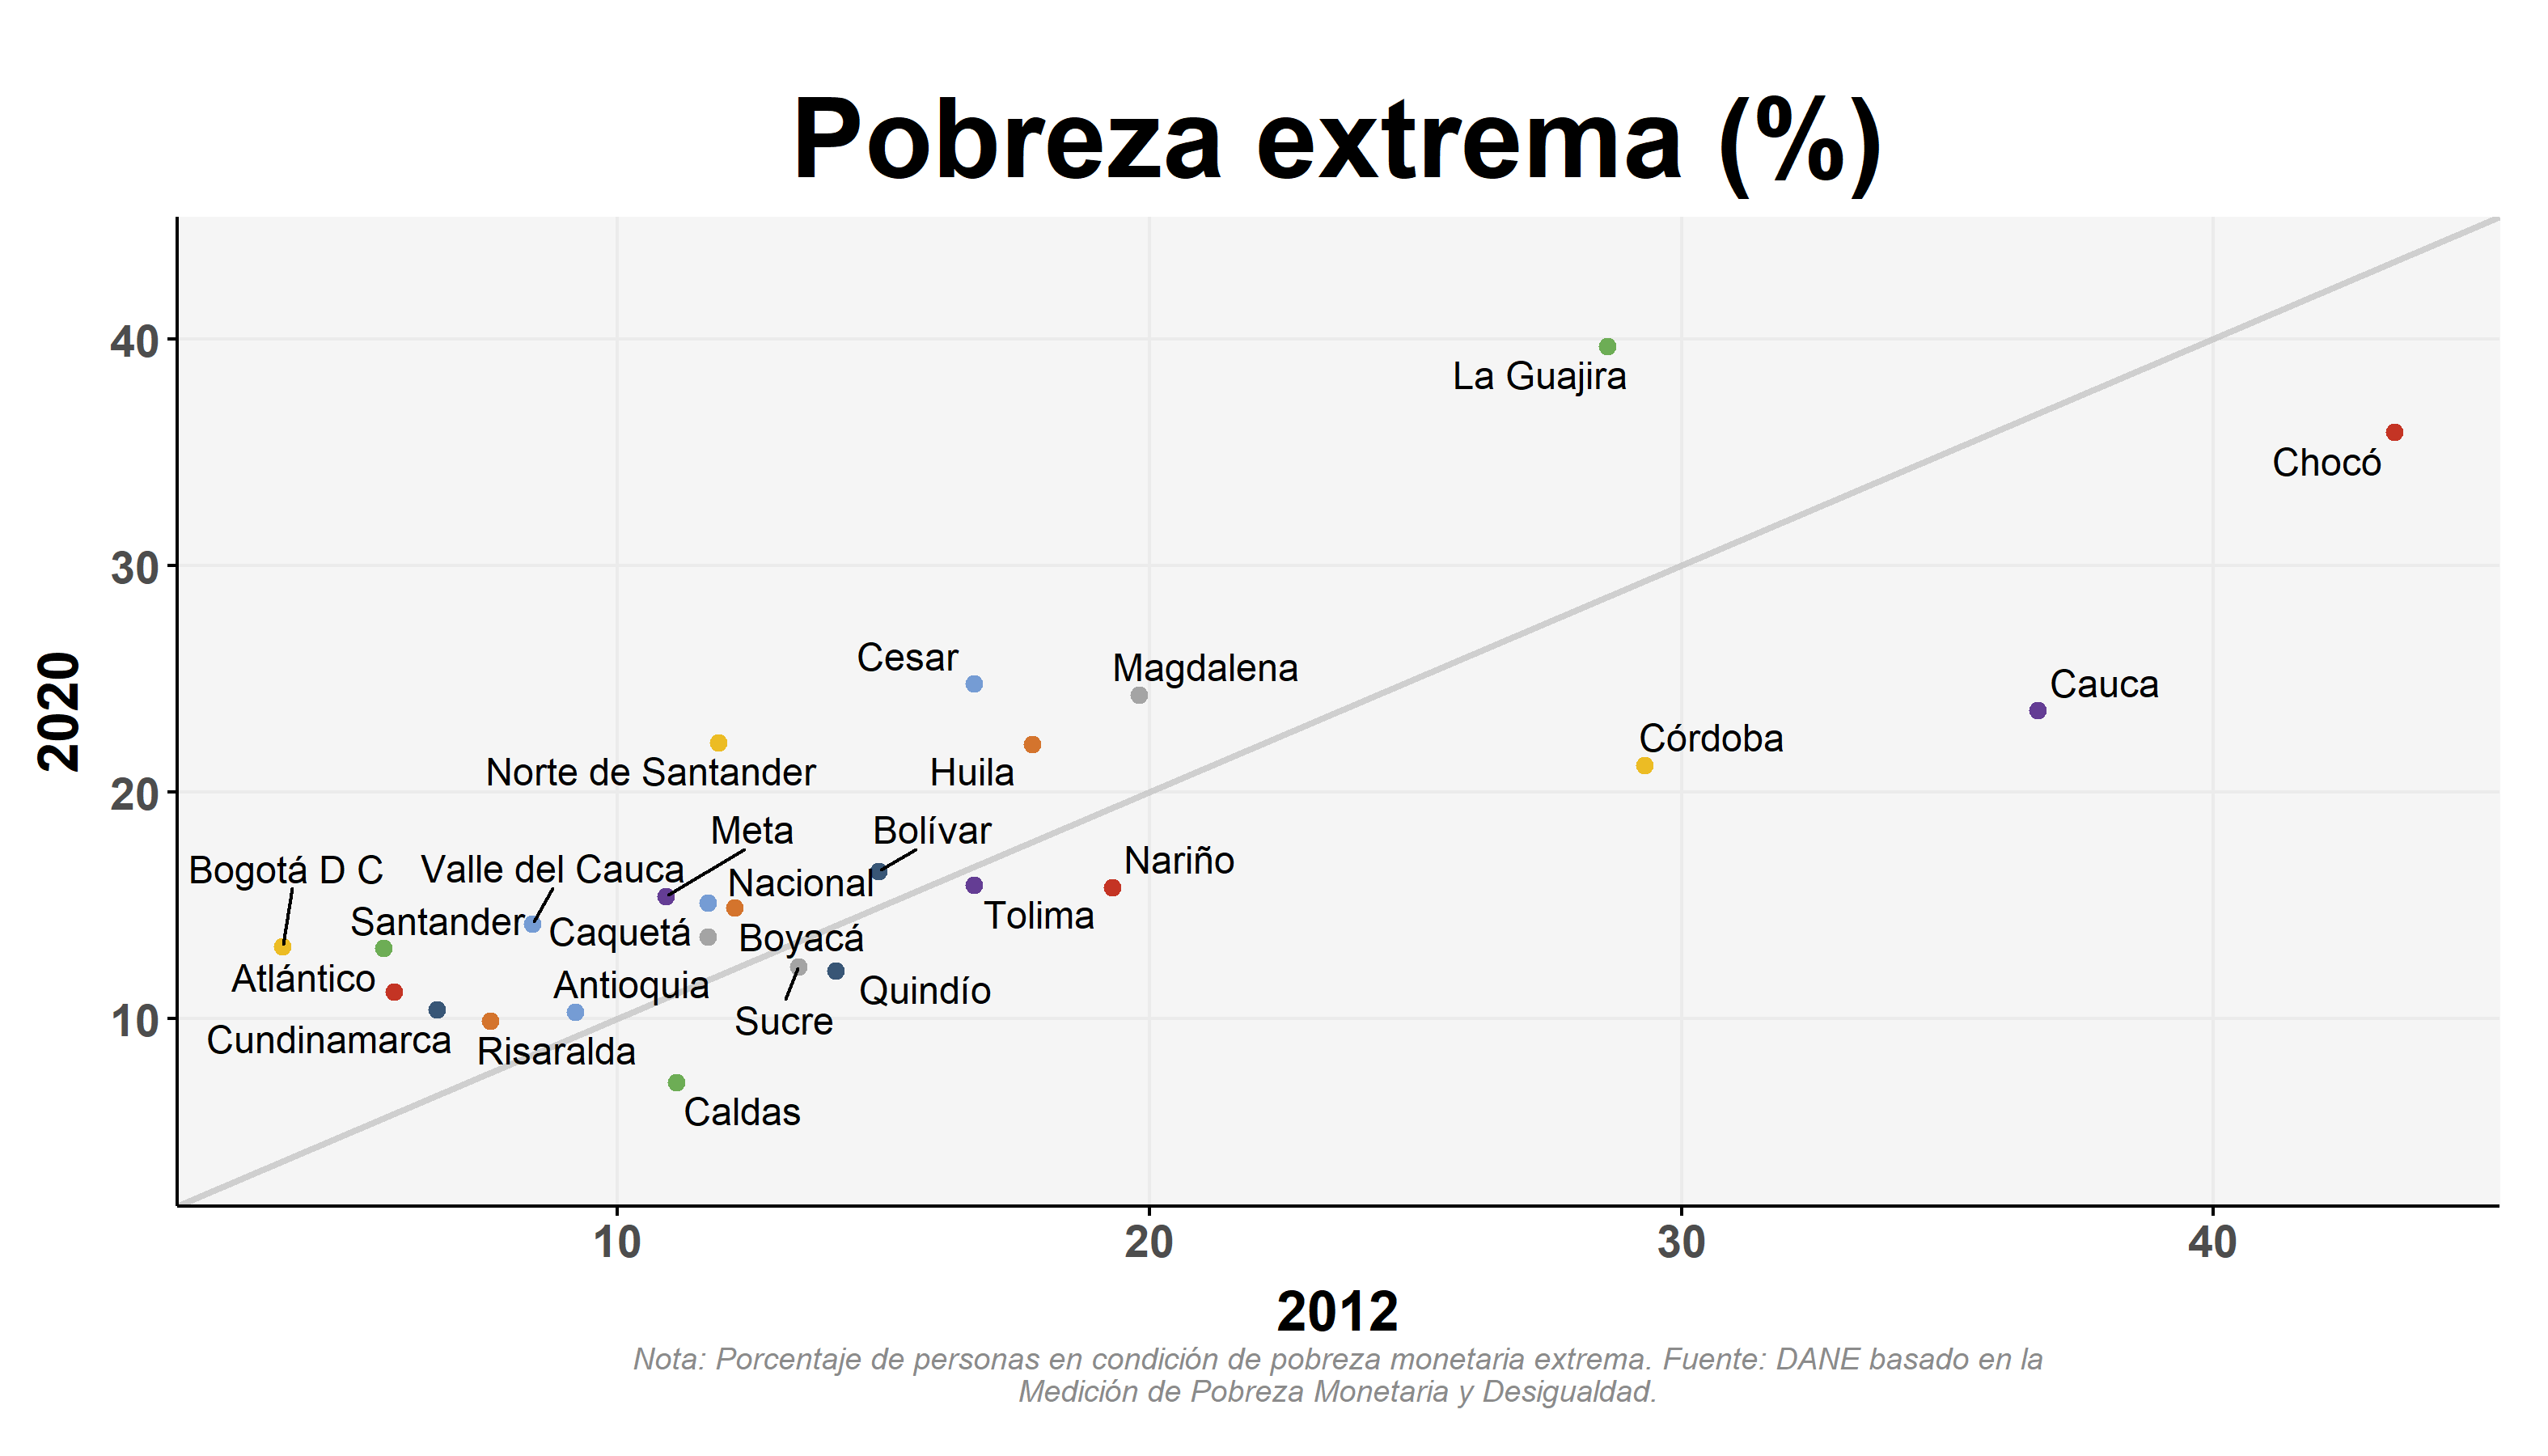
\includegraphics[width=\textwidth,keepaspectratio]{img/var_258_scatter_time.png}
        \end{center}
    \end{figure}
            \begin{itemize}
                    \item Departamentos como Chocó, Cauca, Córdoba, Caldas y Nariño presentaron mejoras significativas para el 2020 comparado con los presentados en 2012.
                    \item Antioquia, Sucre y Tolima mantuvieron niveles de pobreza extrema similares entre 2012 y 2020.
                    \item Gran parte de los departamentos obtuvieron registros superiores para 2020 comparado con los del 2012, la mayoría se concentran entre el 10 y 20\% de pobreza extrema.
                    \item La Guajira y Chocó son los departamentos con los mayores niveles de pobreza extrema con una diferencia por encima del 10\% con el tercer departamento en fila.
                    \end{itemize}

%%%% Include figures
    \begin{figure}[H]
        \caption[Pobreza extrema por departamentos - Cambio porcentual entre 2012 y 2020 ]{\label{pobreza_extrema_dptos_cambio} }
        \begin{center}
        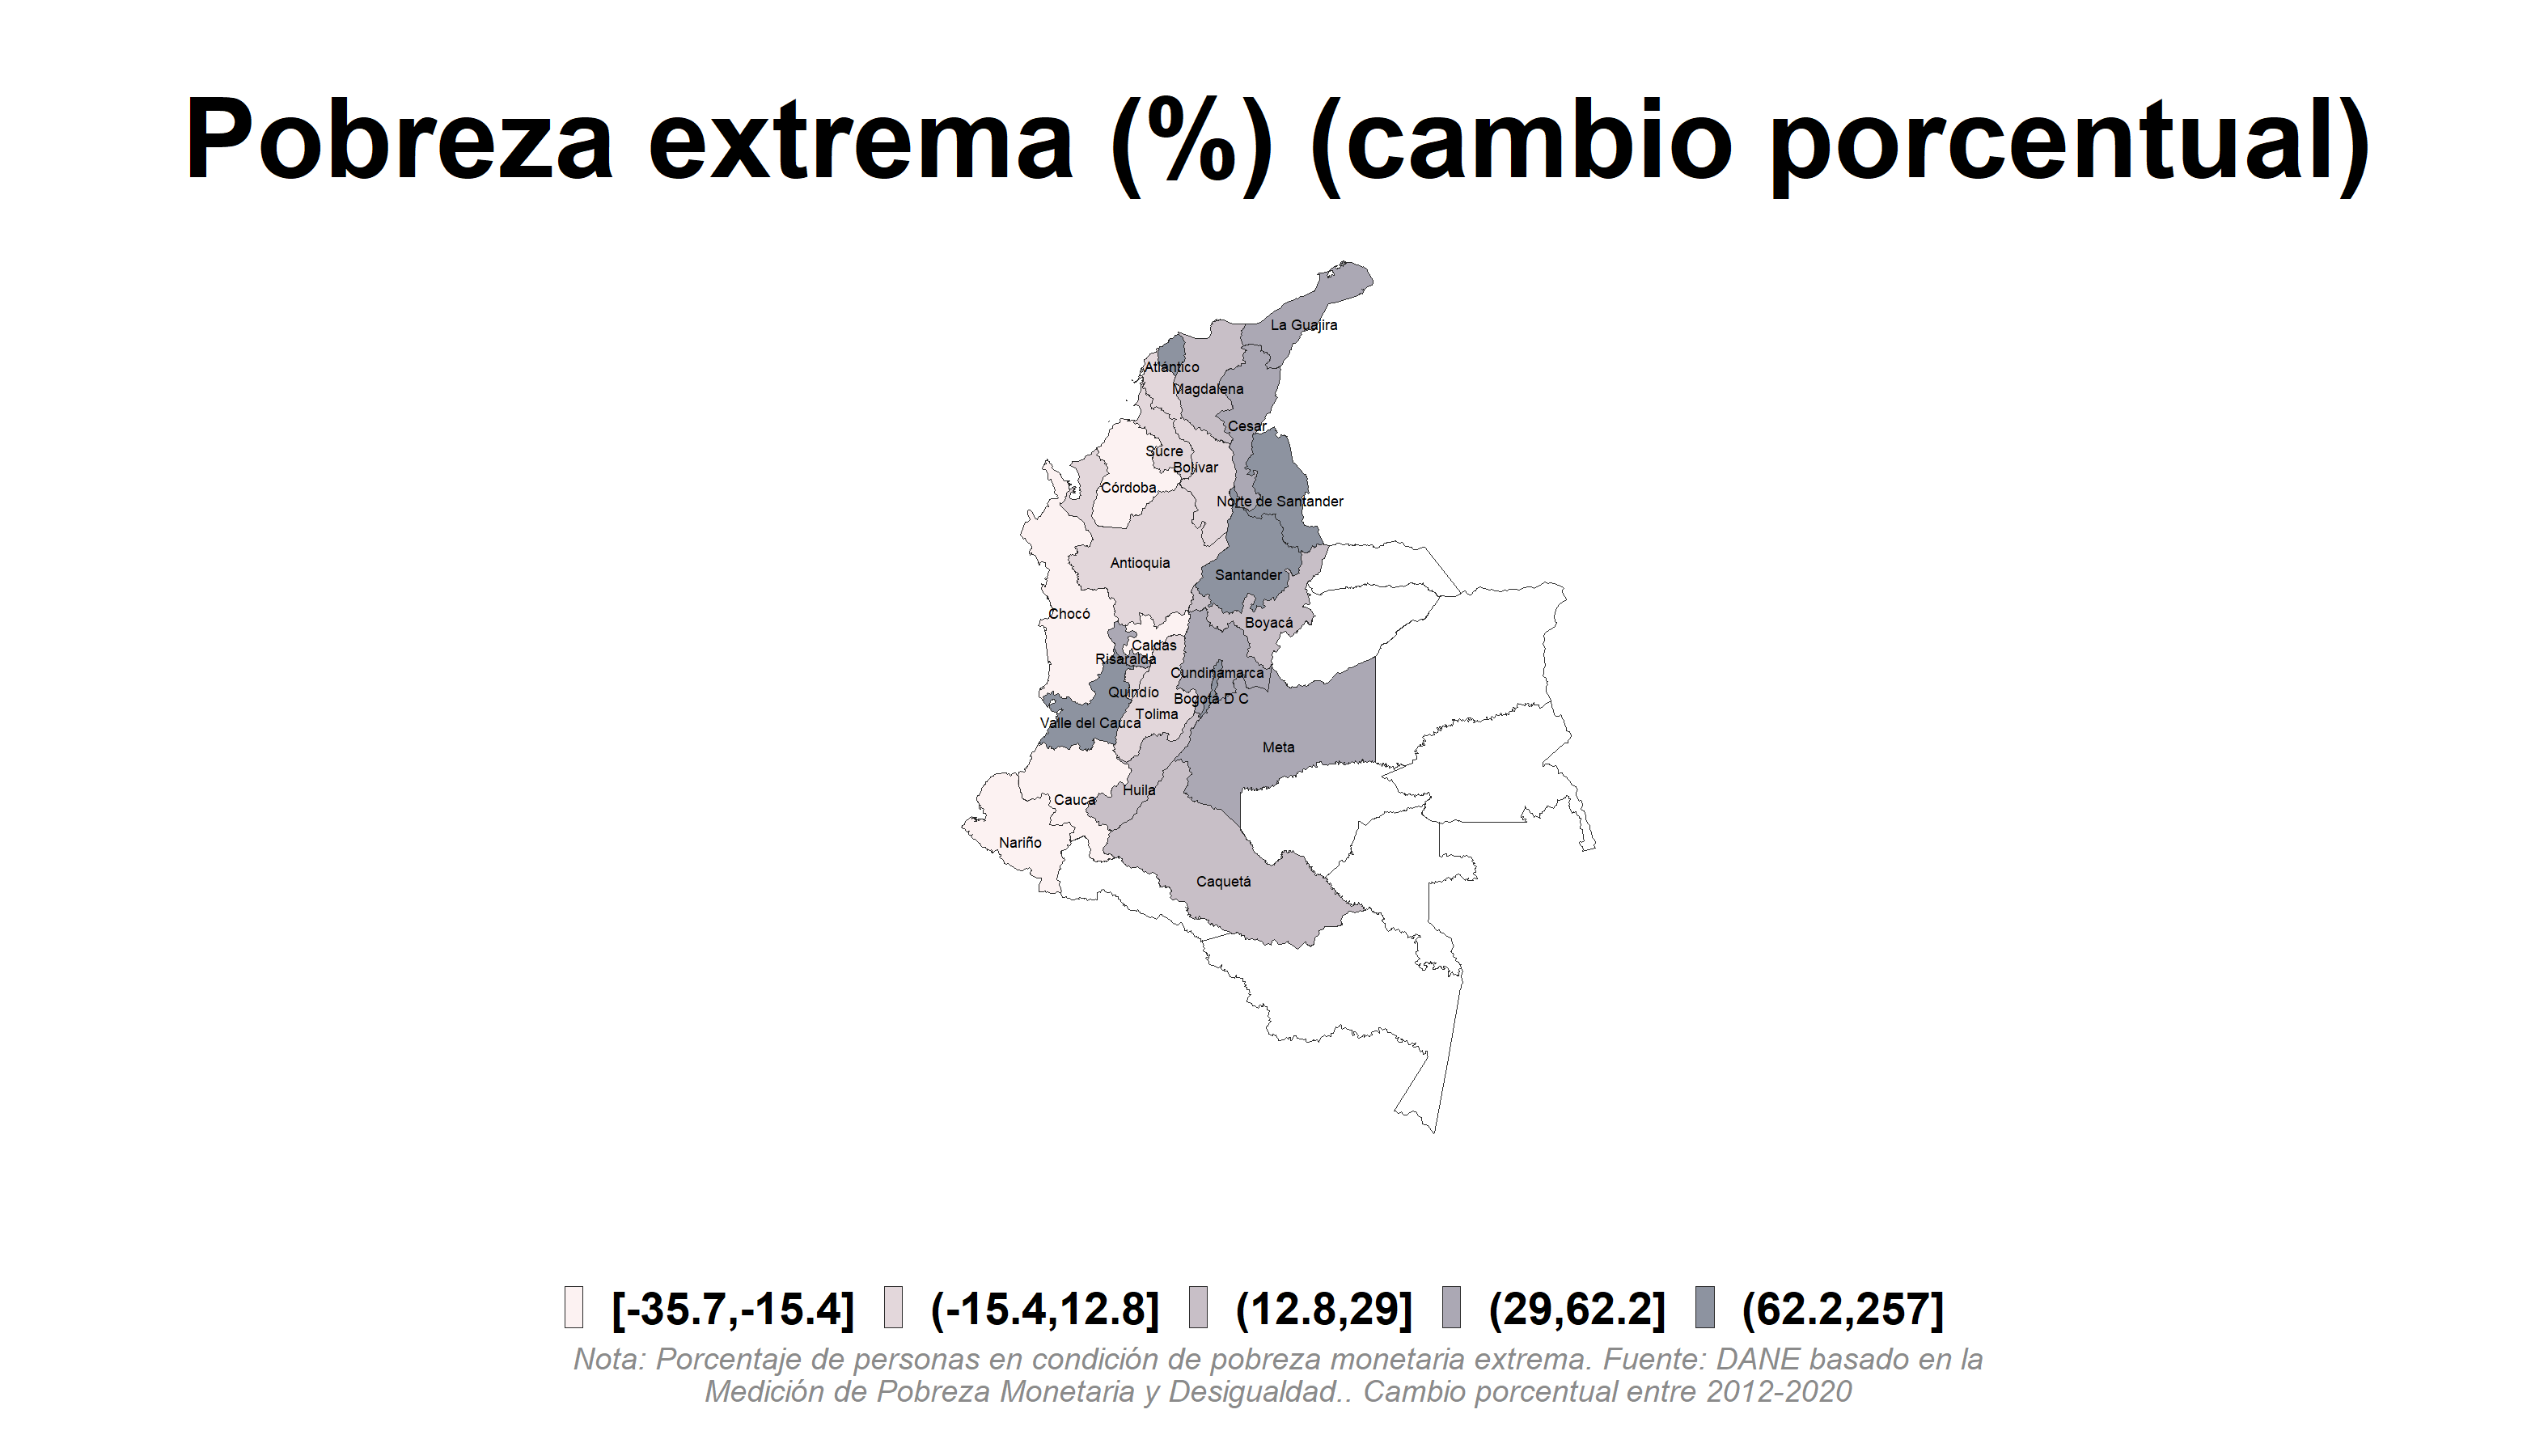
\includegraphics[width=\textwidth,keepaspectratio]{img/var_258_map_change.png}
        \end{center}
    \end{figure}
            \begin{itemize}
                    \item Chocó, Cauca, Nariño, Córdoba y Caldas muestran mejoras significativas entre los dos años.
                    \item Santander, Norte de Santander, Valle, Atlántico y Bogotá son los que presentan los mayores rangos de aumento de pobreza extrema entre los 2 años.
                    \end{itemize}

%%%% Include figures
    \begin{figure}[H]
        \caption[Pobreza extrema por zonas y nacional ]{\label{pobreza_extrema_zonas} }
        \begin{center}
        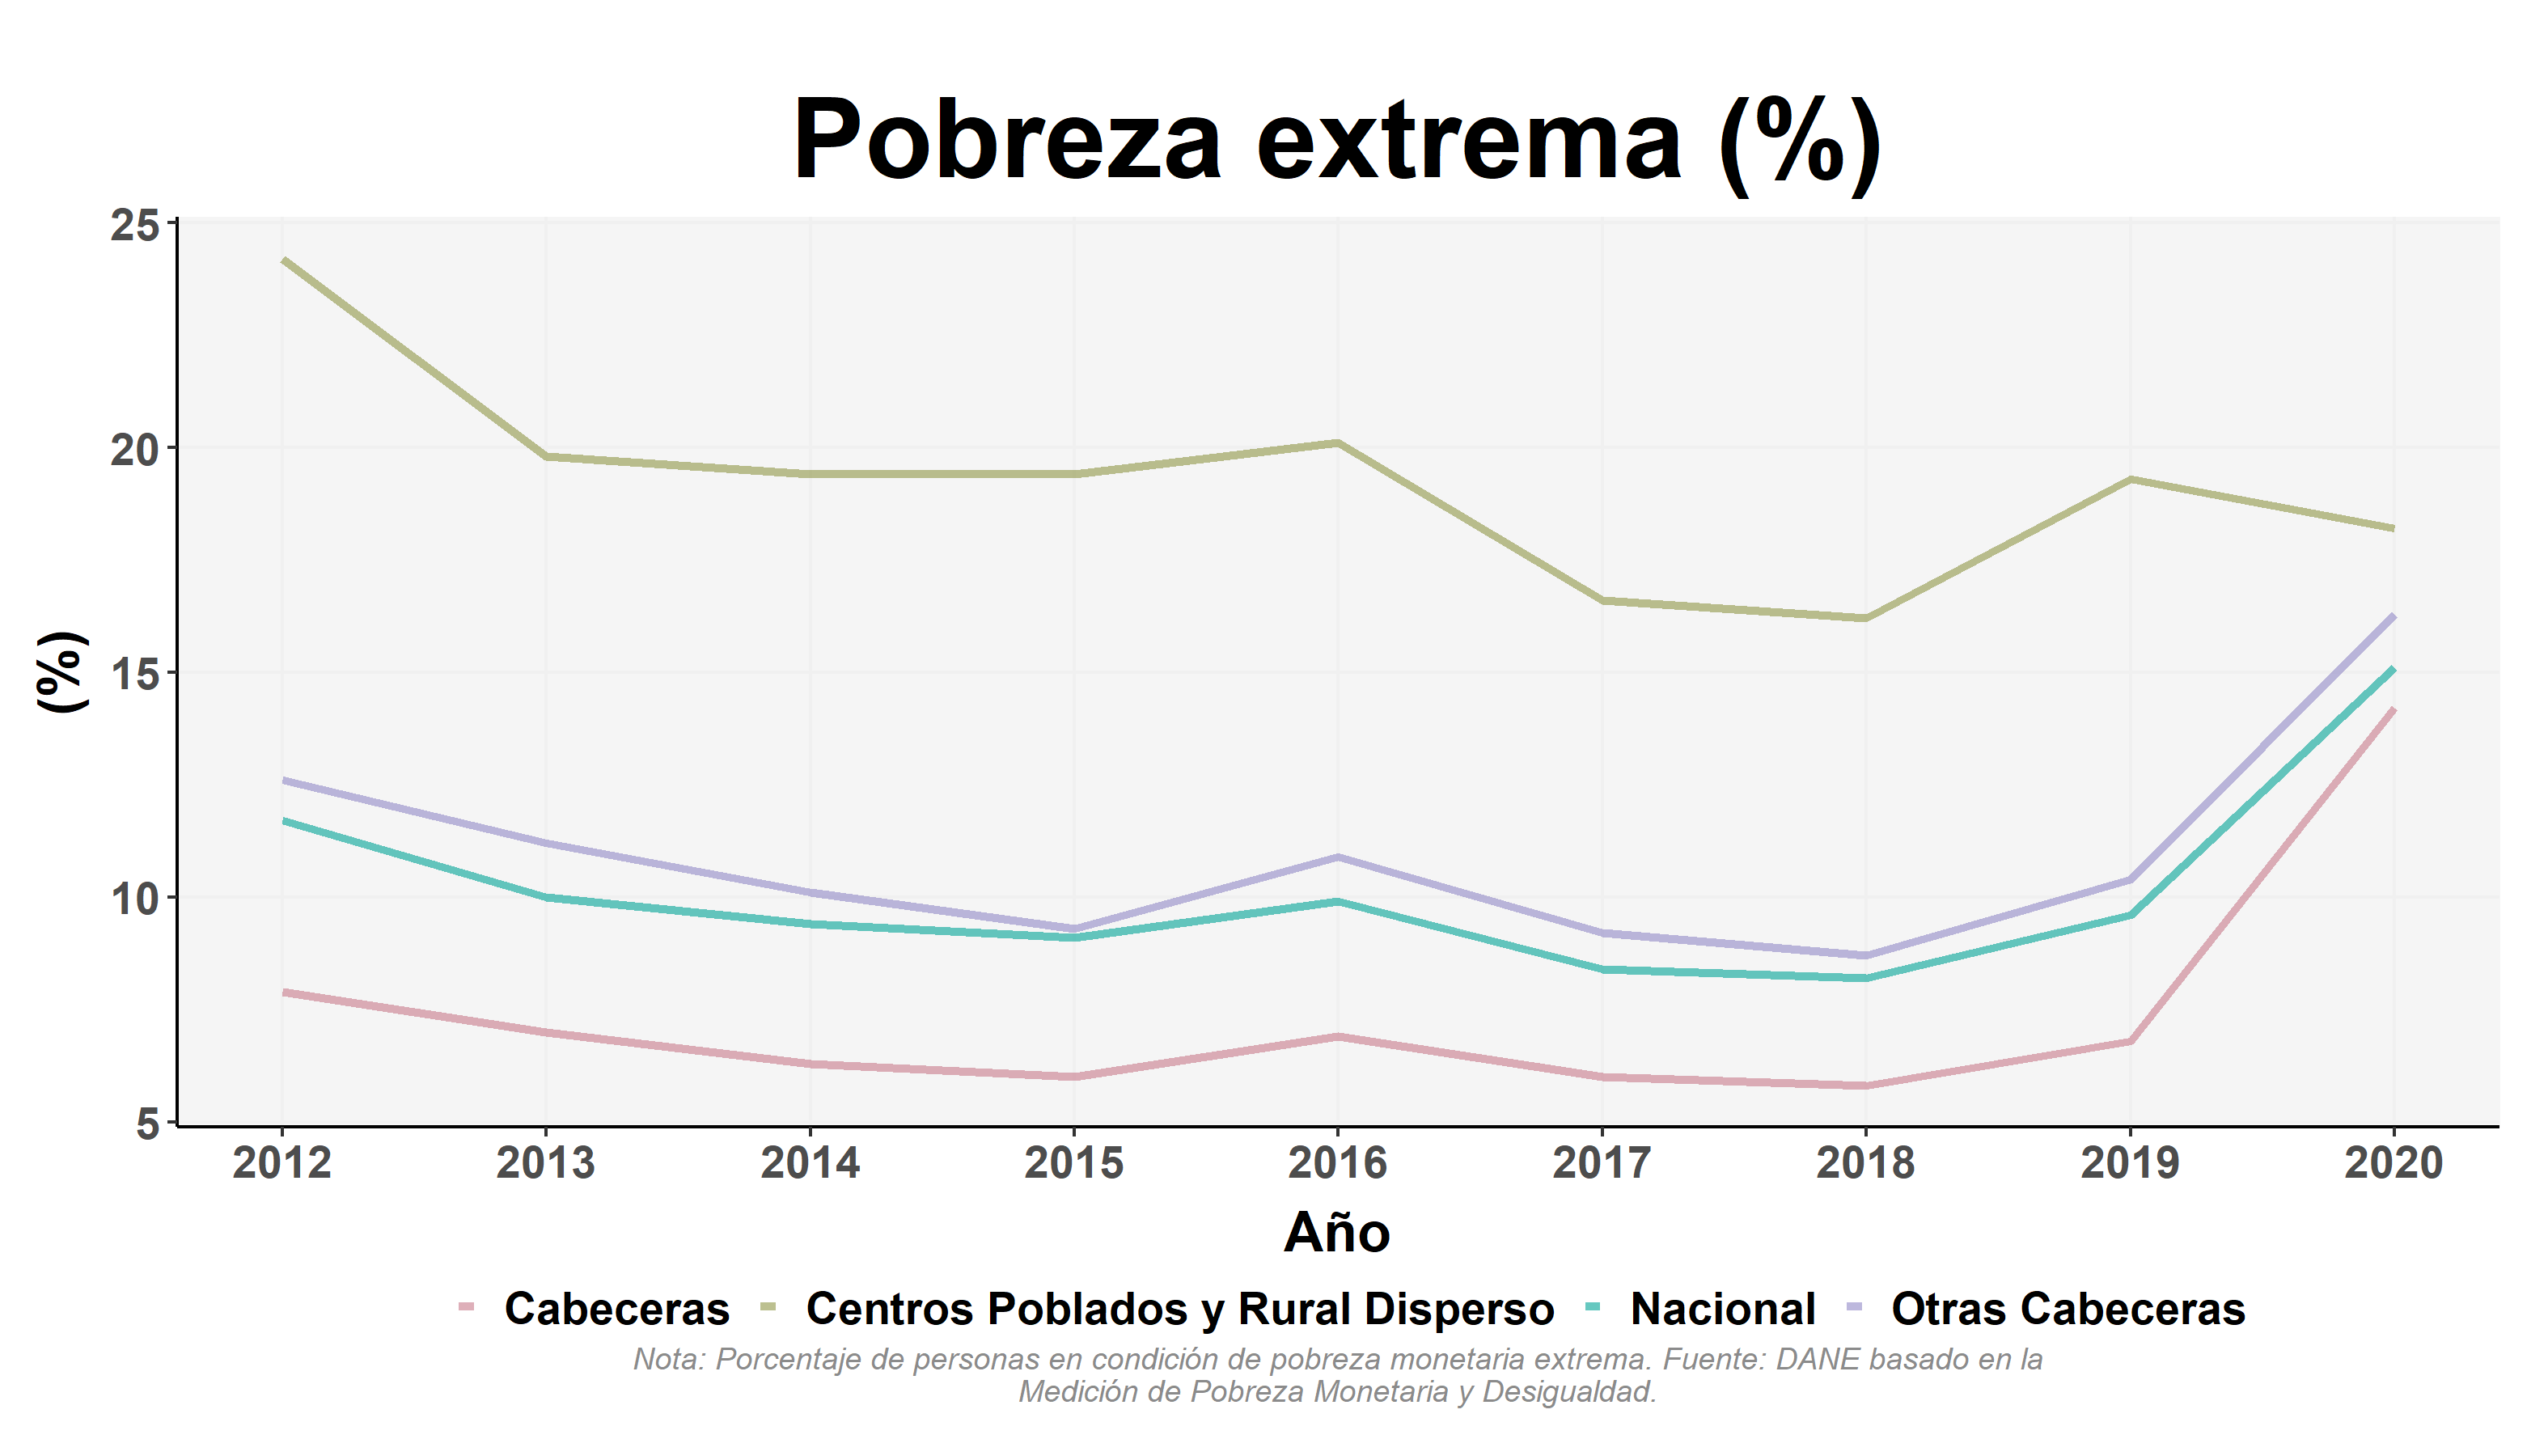
\includegraphics[width=\textwidth,keepaspectratio]{img/var_260_trend.png}
        \end{center}
    \end{figure}
            \begin{itemize}
                    \item Los niveles de pobreza extrema estaban disminuyendo, con un leve pico en 2016, hasta 2018.
                    \item Desde el 2019 se inicio un crecimiento, intensificado en el 2020 pero caso contrario con los centros poblados y rural donde en el 2020 disminuyó.
                    \item Se disminuyó la brecha entre a zona rural y las otras zonas, acercándose para el 2020.
                    \item Para las cabeceras, a nivel nacional y las otras cabeceras se registraron para 2020 valores superiores que los del 2012, caso contrario con las zonas rurales. 
                    \end{itemize}

\subsubsection{Pobreza Monetaria}

%%%% Include figures
    \begin{figure}[H]
        \caption[Pobreza monetaria por ciudades - 2012 VS 2020 ]{\label{pobreza_monetaria_ciudades_vs} }
        \begin{center}
        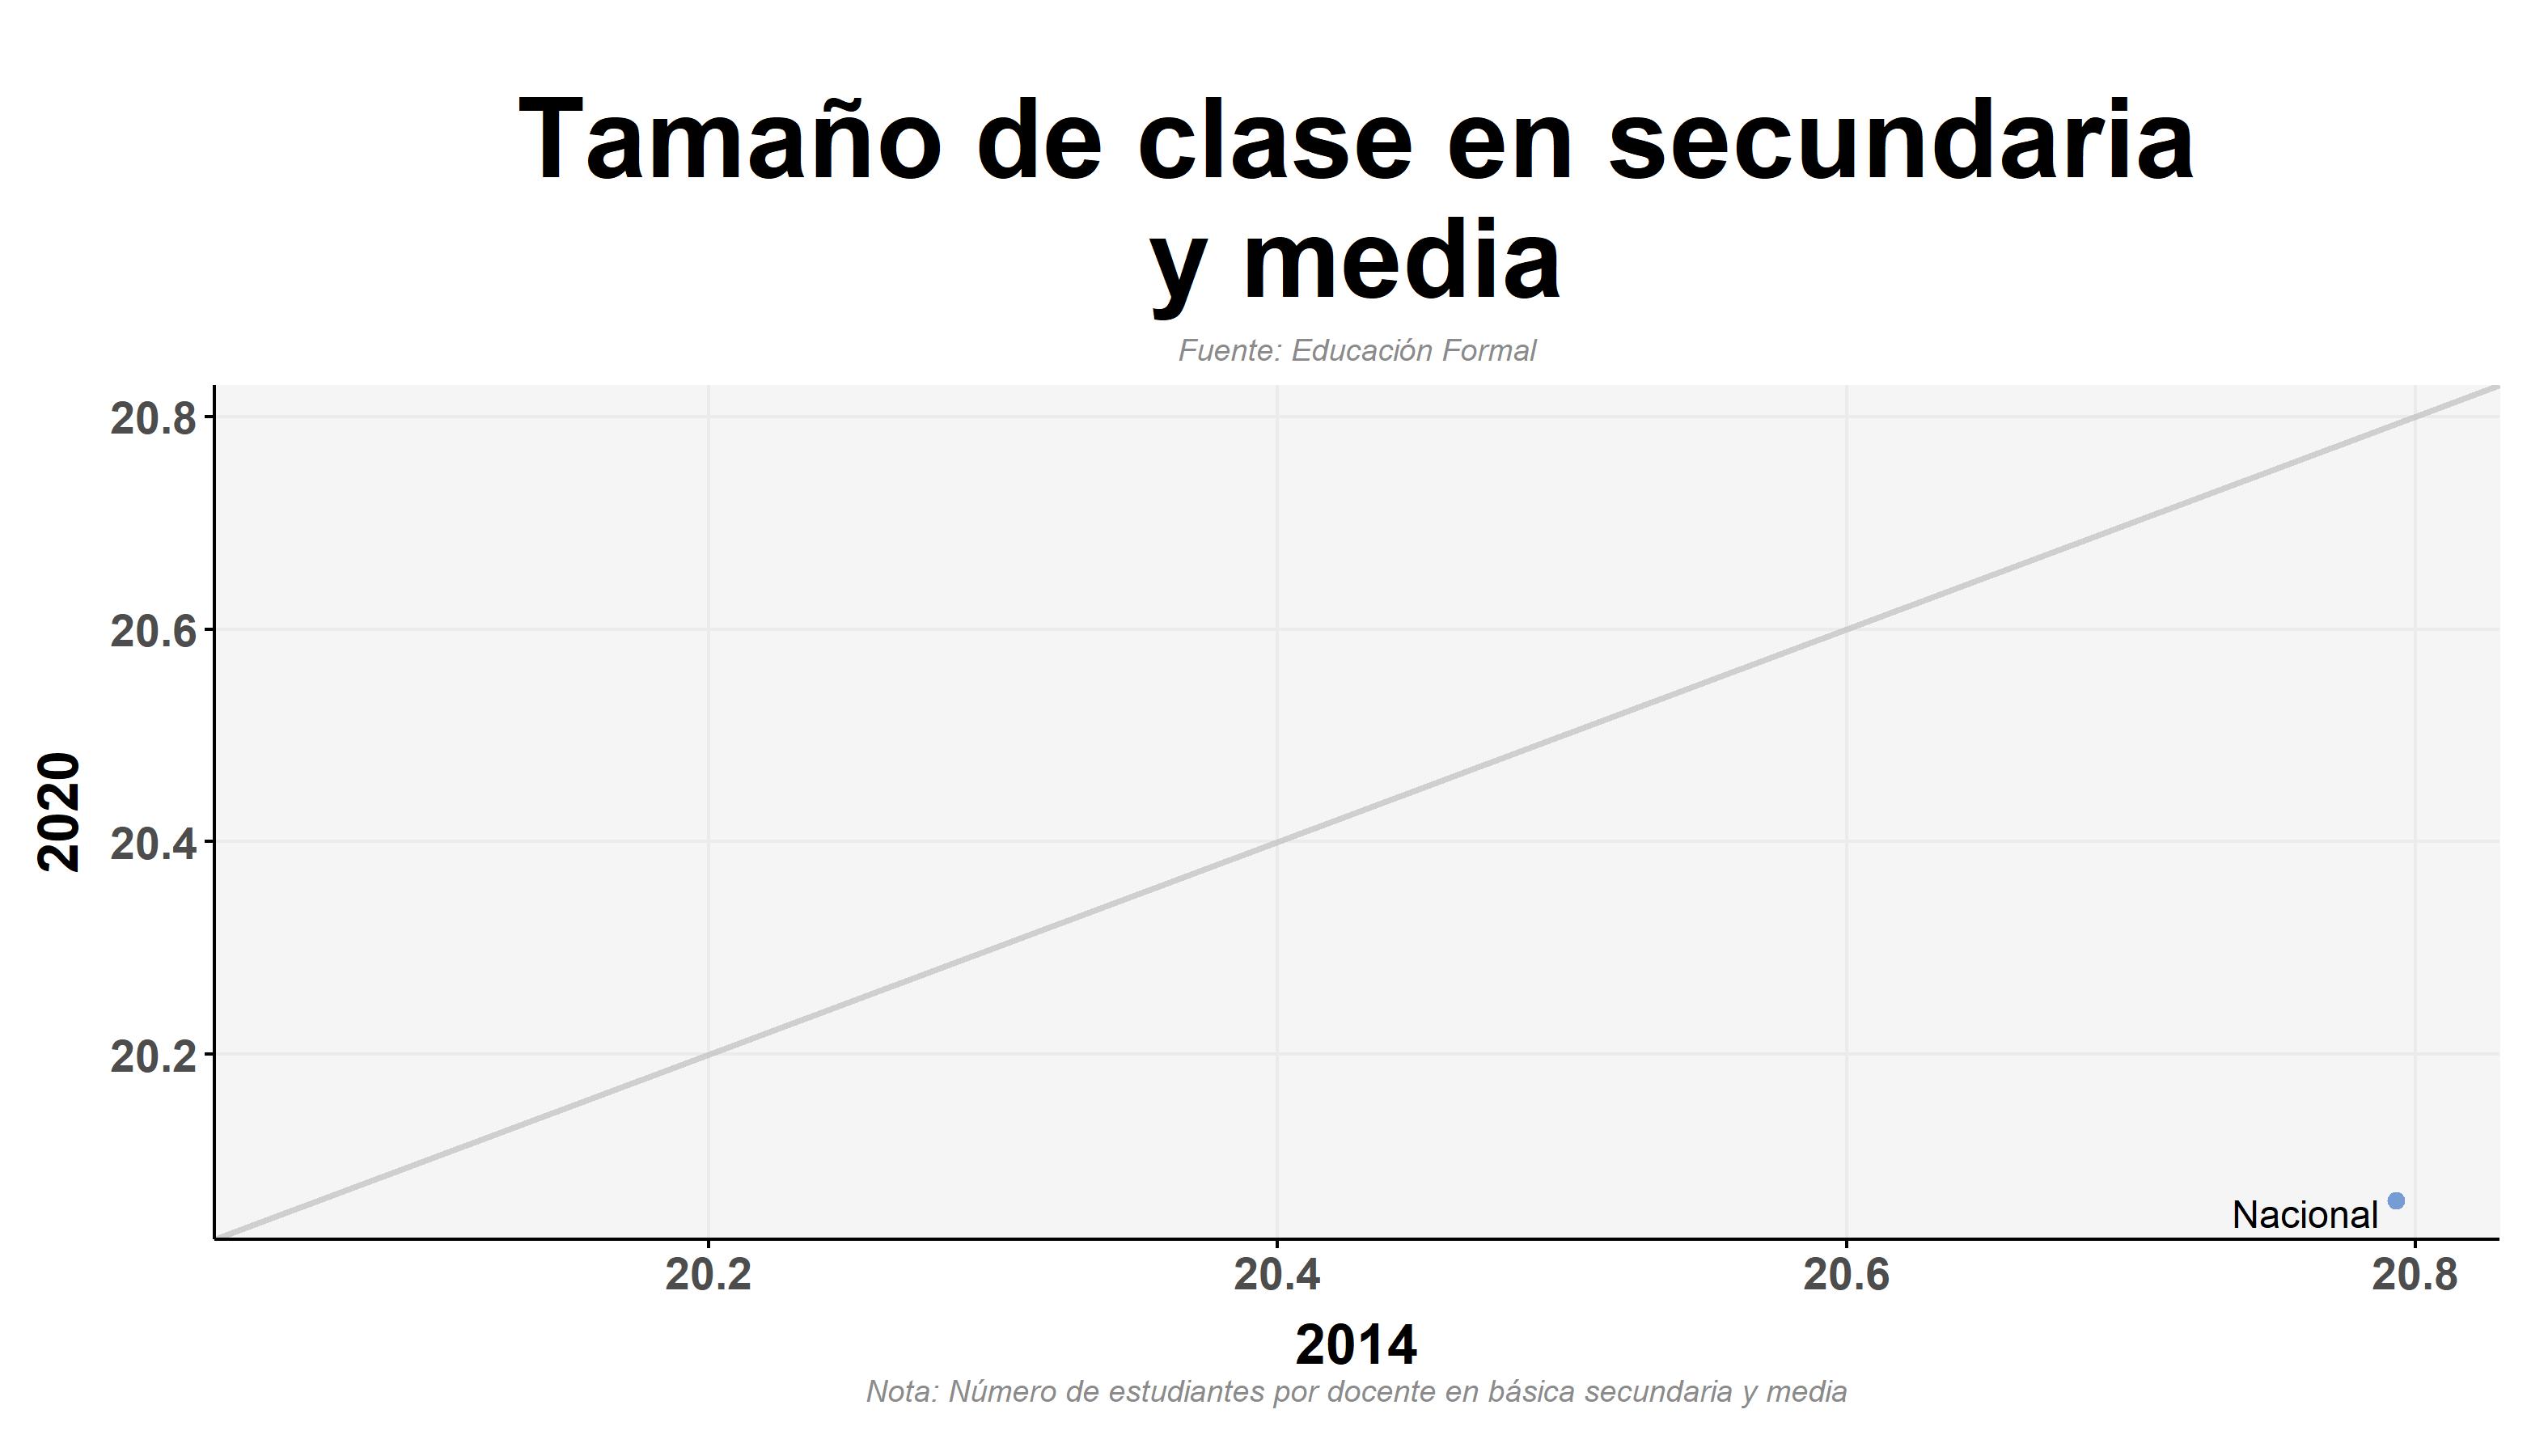
\includegraphics[width=\textwidth,keepaspectratio]{img/var_261_scatter_time.png}
        \end{center}
    \end{figure}
            \begin{itemize}
                    \item Pasto es la única ciudad que mejoró sus niveles de pobreza monetaria en 2020 con respecto al 2012, las demás ciudades tuvieron valores más altos.
                    \item Todas las ciudades están por encima del 30\% de la población en pobreza monetaria, Cúcuta es la única que pasa del 50\% de su población viviendo con pobreza monetaria.
                    \item Bucaramanga paso de ser la ciudad con el menor nivel de pobreza monetaria en 2012, cerca del 20\%, a ser la cuarta ciudad con mayor nivel de población en pobreza monetaria con niveles por encima del 45\%.
                    \item Entre las ciudades extremo hay una diferencia aproximada del 20\% (Manizales - Cúcuta).
                    \end{itemize}

%%%% Include figures
    \begin{figure}[H]
        \caption[Pobreza monetaria por departamentos - 2012 VS 2020 ]{\label{pobreza_monetaria_dptos_vs} }
        \begin{center}
        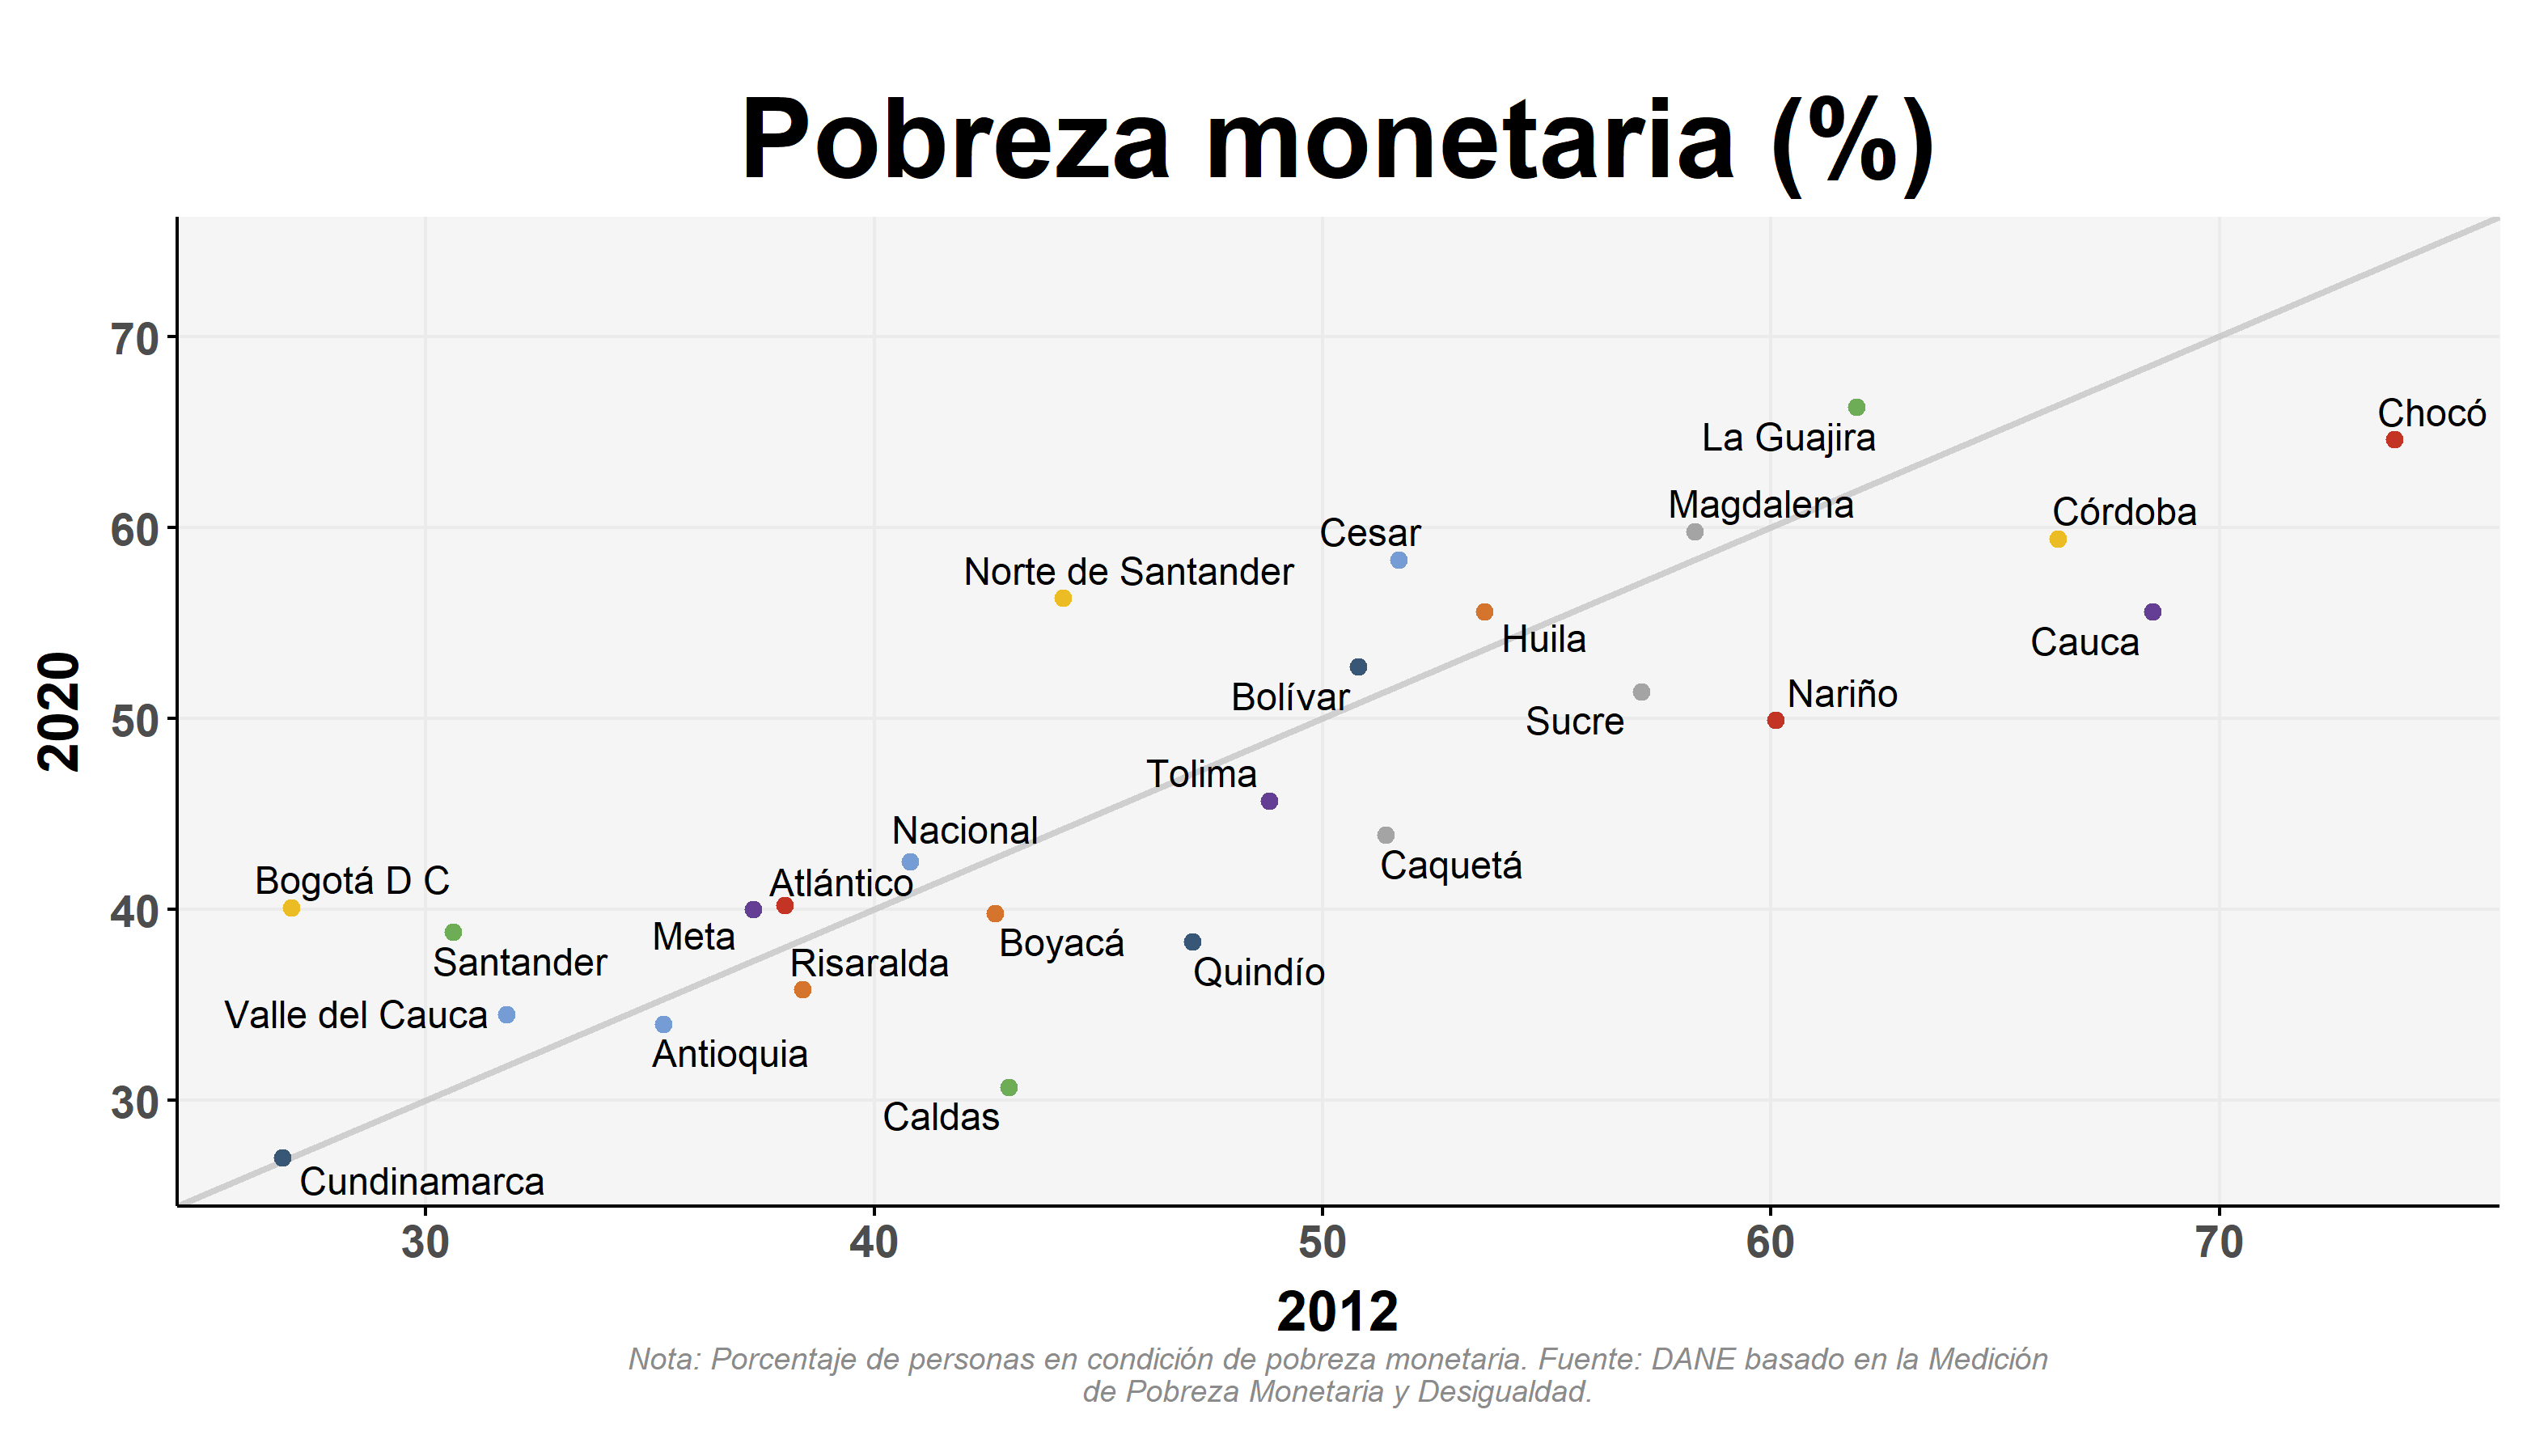
\includegraphics[width=\textwidth,keepaspectratio]{img/var_262_scatter_time.png}
        \end{center}
    \end{figure}
            \begin{itemize}
                    \item La mitad de los departamentos tuvieron mejoras en el 2020 con respecto al 2012.
                    \item Chocó a pesar de haber mejorado se mantiene como el segundo dpto con mayor pobreza en 2020, en 2012 fue el primero.
                    \item La diferencia entre los dptos extremo es del aproximadamente el 40\% (Cundinamarca - La Guajira).
                    \item Vemos que la distribución de lugares no ha cambiado drásticamente y la de valores tienen una amplia distribución.
                    \end{itemize}

%%%% Include figures
    \begin{figure}[H]
        \caption[Pobreza monetaria por departamentos - Cambio porcentual entre 2012 y 2020 ]{\label{pobreza_monetaria_dptos_cambio} }
        \begin{center}
        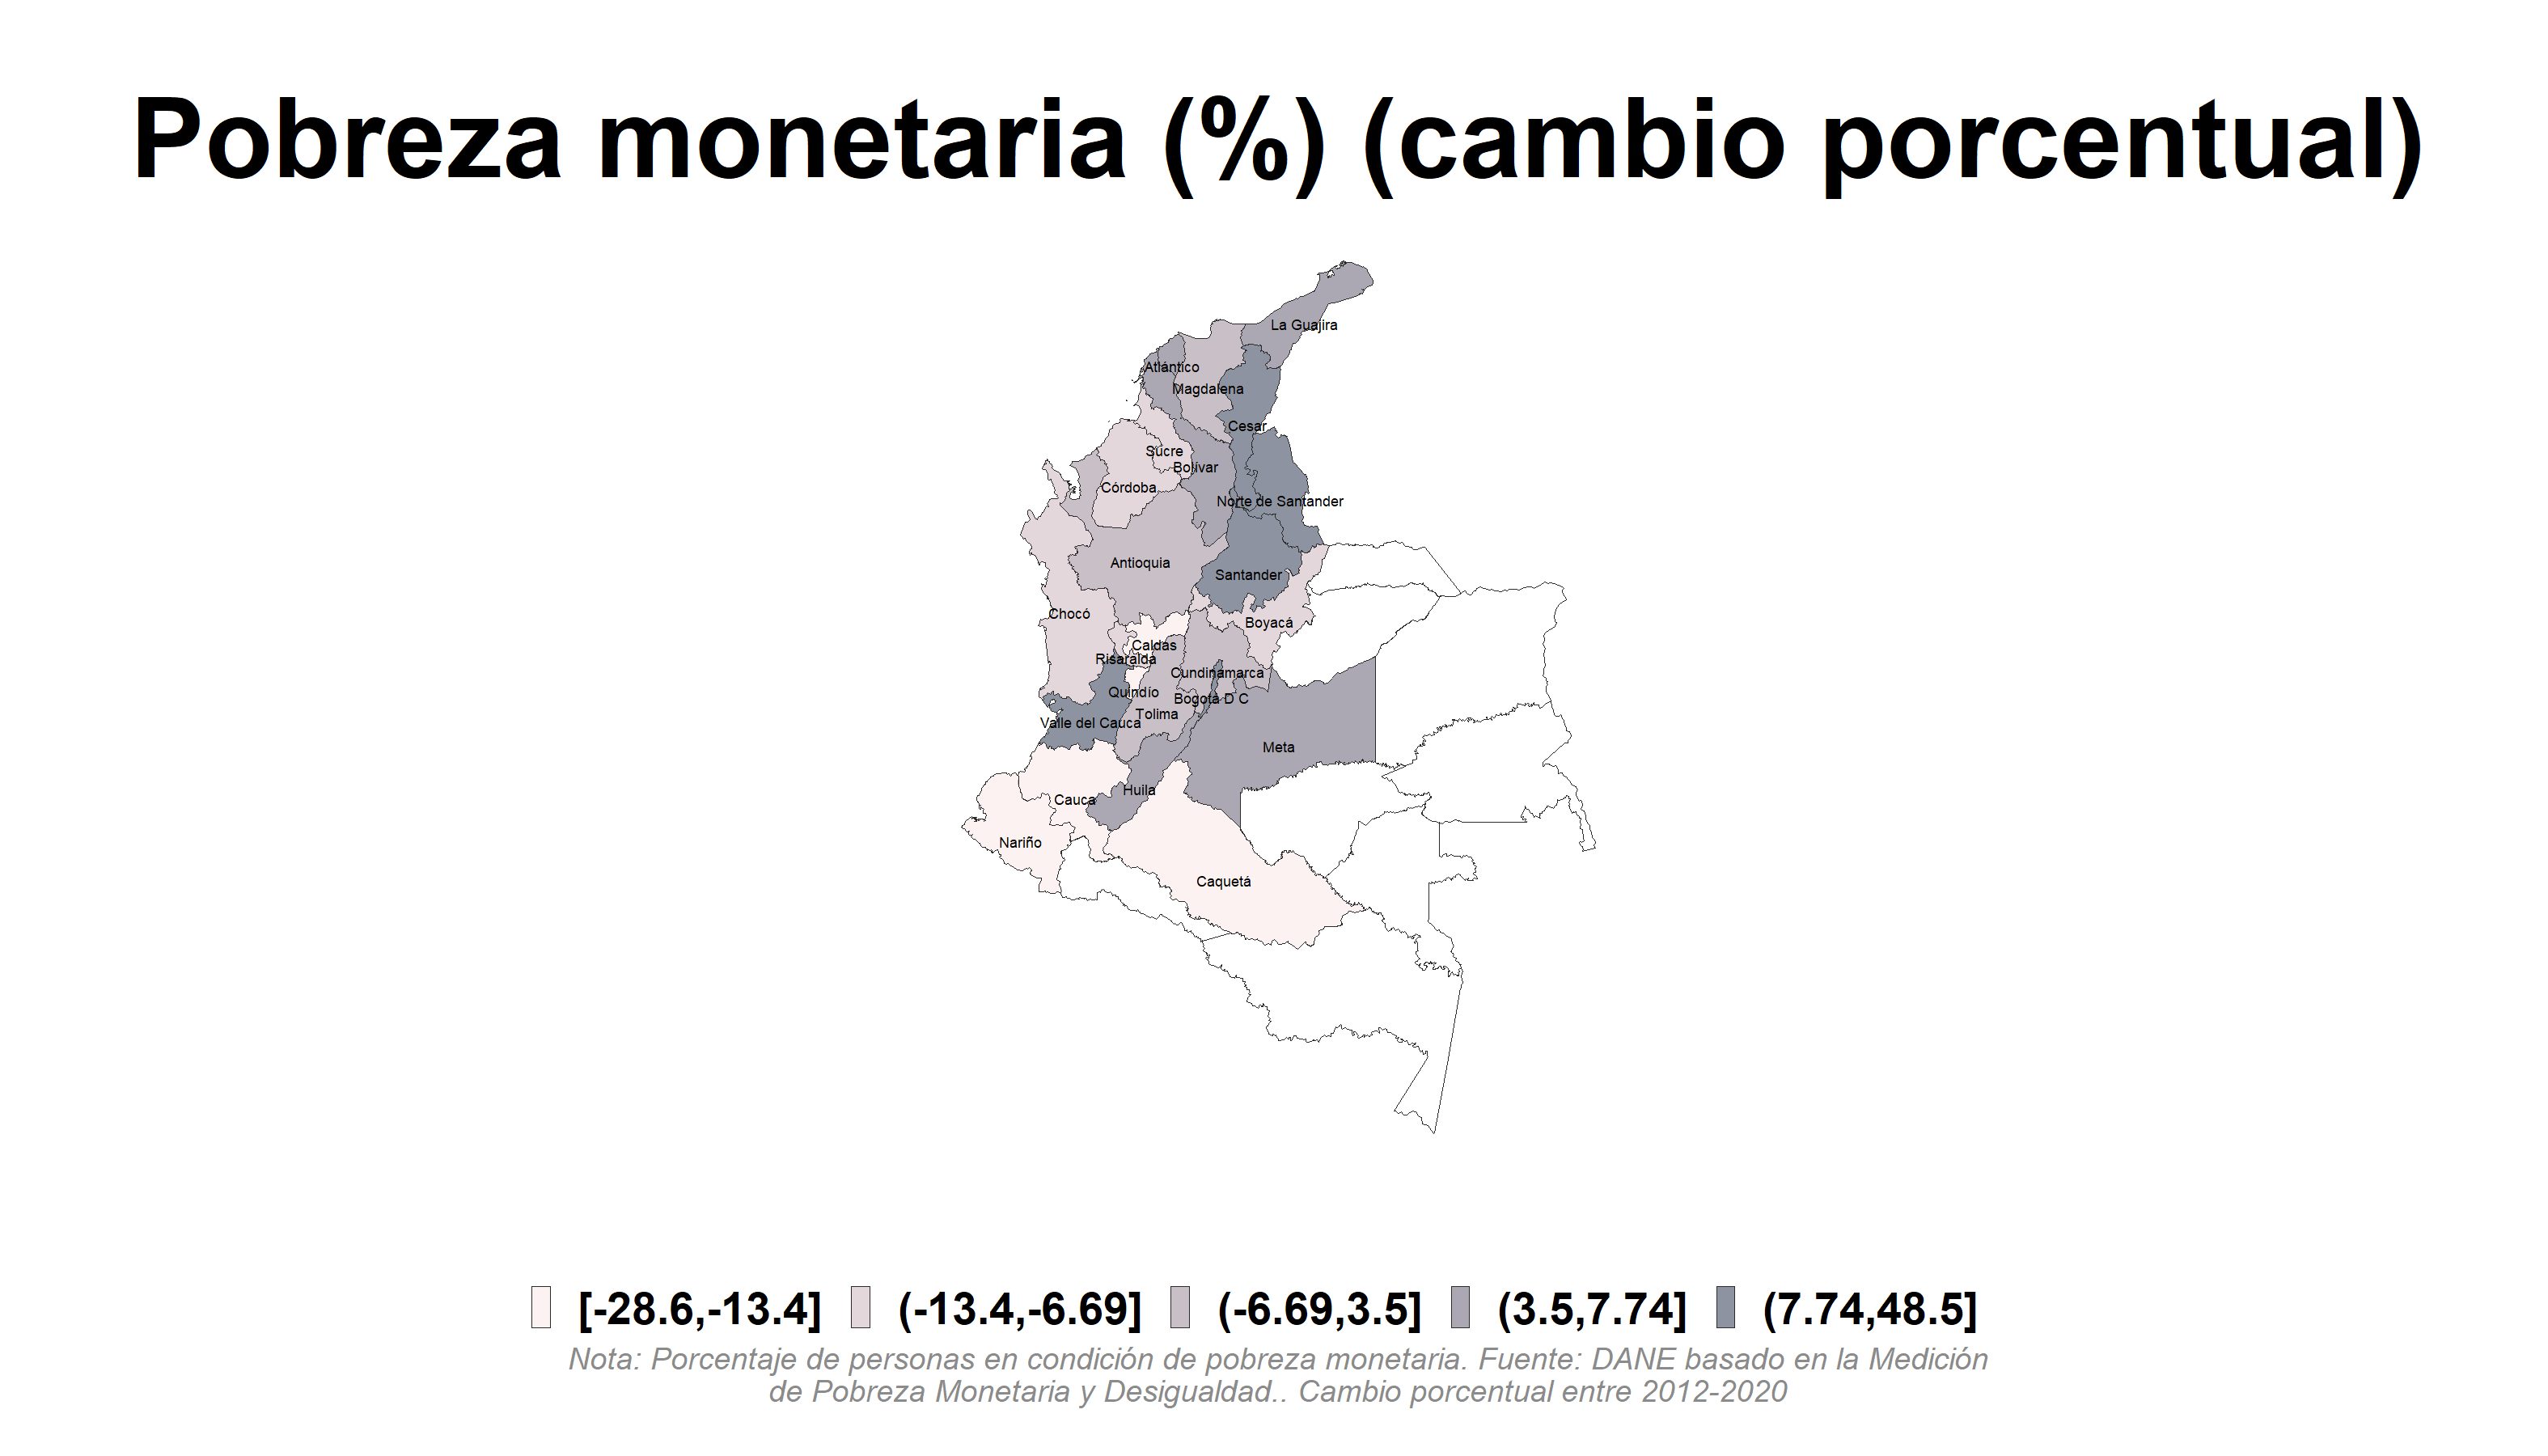
\includegraphics[width=\textwidth,keepaspectratio]{img/var_262_map_change.png}
        \end{center}
    \end{figure}
            \begin{itemize}
                    \item Cauca, Quindío, Caldas, Nariño y Caquetá son los departamentos que muestran una mayor mejoría con diferencias por encima del 13\% entre 2012 y 2020.
                    \item Los departamentos que más desmejoraron para el 2020 son Santander, Norte, Cesar y Valle, también se añade Bogotá que pasó de tener niveles por debajo del 20\% al 40\%.
                    \end{itemize}

%%%% Include figures
    \begin{figure}[H]
        \caption[Pobreza monetaria por zonas y nacional ]{\label{pobreza_monetaria_zonas} }
        \begin{center}
        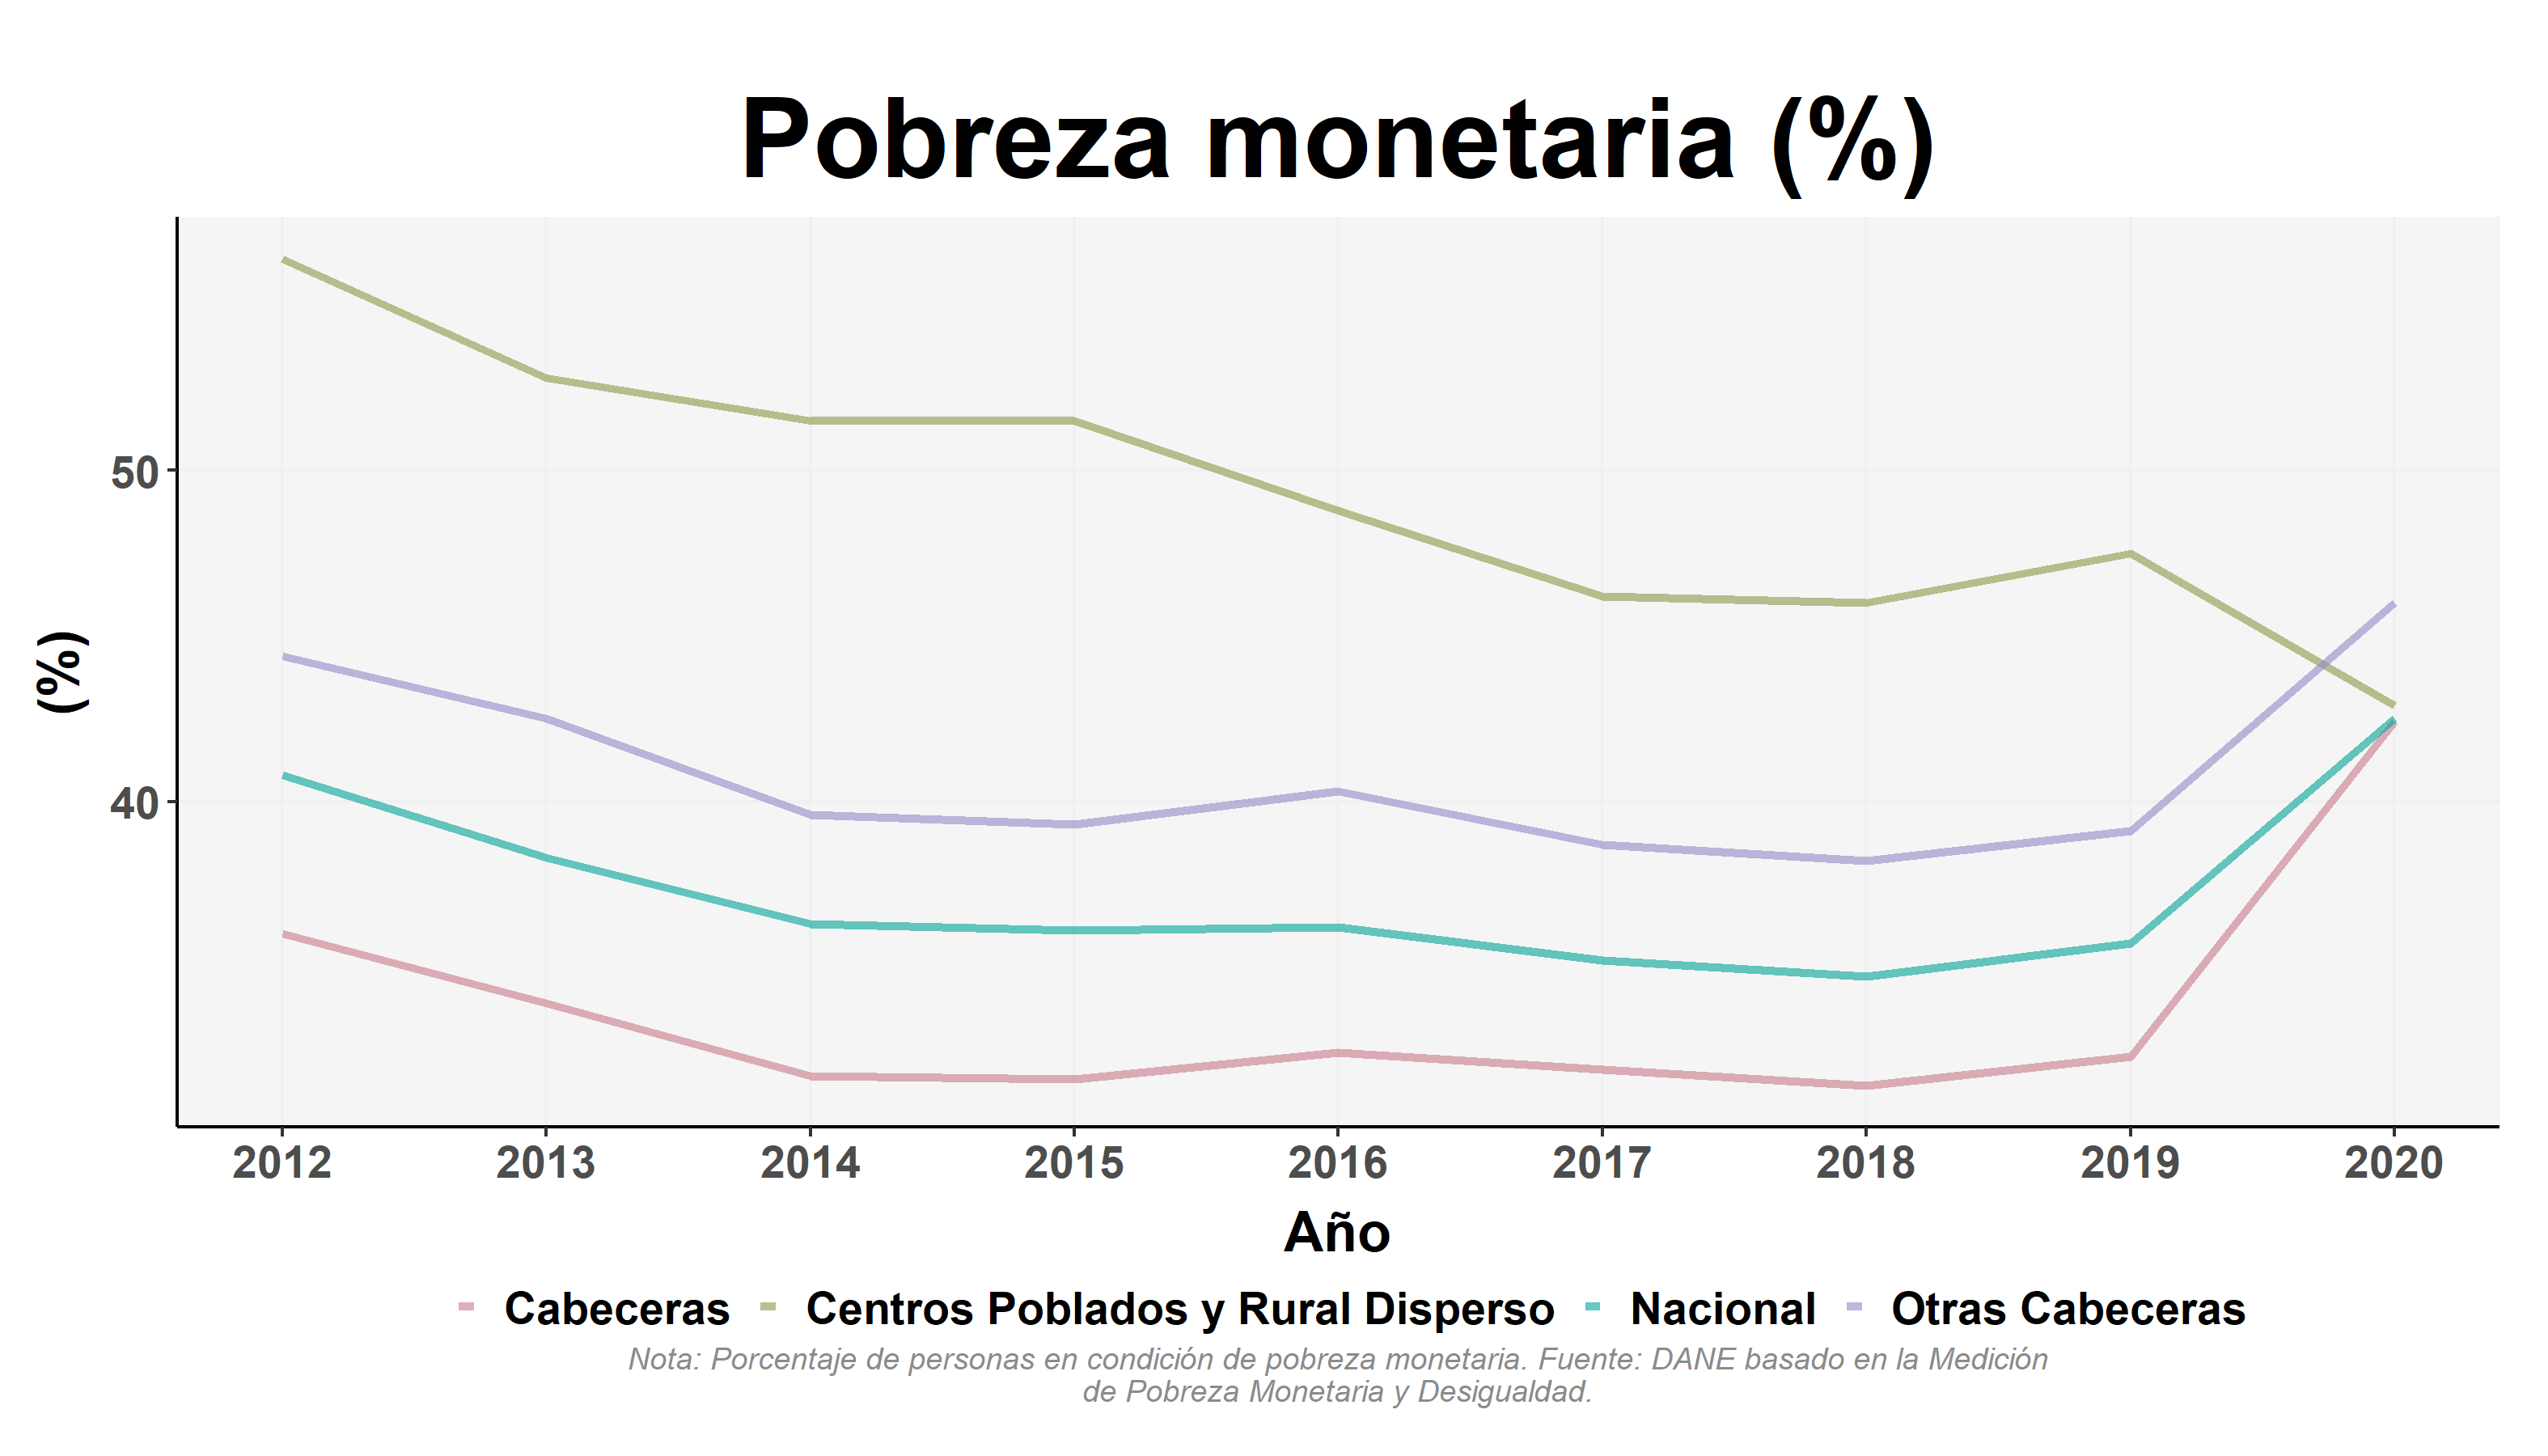
\includegraphics[width=\textwidth,keepaspectratio]{img/var_264_trend.png}
        \end{center}
    \end{figure}
            \begin{itemize}
                    \item La tendencia de los últimos 9 años muestra que la pobreza monetaria estaba descendiendo hasta el 2018, con picos en el 2016 para las cabeceras y las otras cabeceras.
                    \item La tendencia para la zona rural es la única que muestra un descenso en el 2020, el resto tienen un aumento que venía desde el 2019 y se intensifico en el 2020.
                    \item Para el 2020 el porcentaje de personas en pobreza monetaria para el nacional y las cabeceras están casi al mismo nivel que el registrado para la zona rural.
                    \item La brecha entre los valores de las cabeceras y la zona rural pasó de ser más del 15\% para el 2019 a menos del 1\% en 2020.
                    \item Las otras cabeceras sobrepasaron el porcentaje de población en pobreza monetaria registrado en 2020 para las zonas rurales y centros poblados.
                    \item Las cabeceras y a nivel nacional tienen valores similares de pobreza monetaria, 42.4\% y 42.5\% respectivamente.
                    \end{itemize}

    \subsection{Pobreza No Monetaria}

        \subsubsection{Índice de Pobreza Multidimensional - IPM}

%%%% Include figures
    \begin{figure}[H]
        \caption[Índice de Pobreza Multidimensional por departamentos- Cambio porcentual entre 2018 y 2020 ]{\label{ipm_dptos_cambio} }
        \begin{center}
        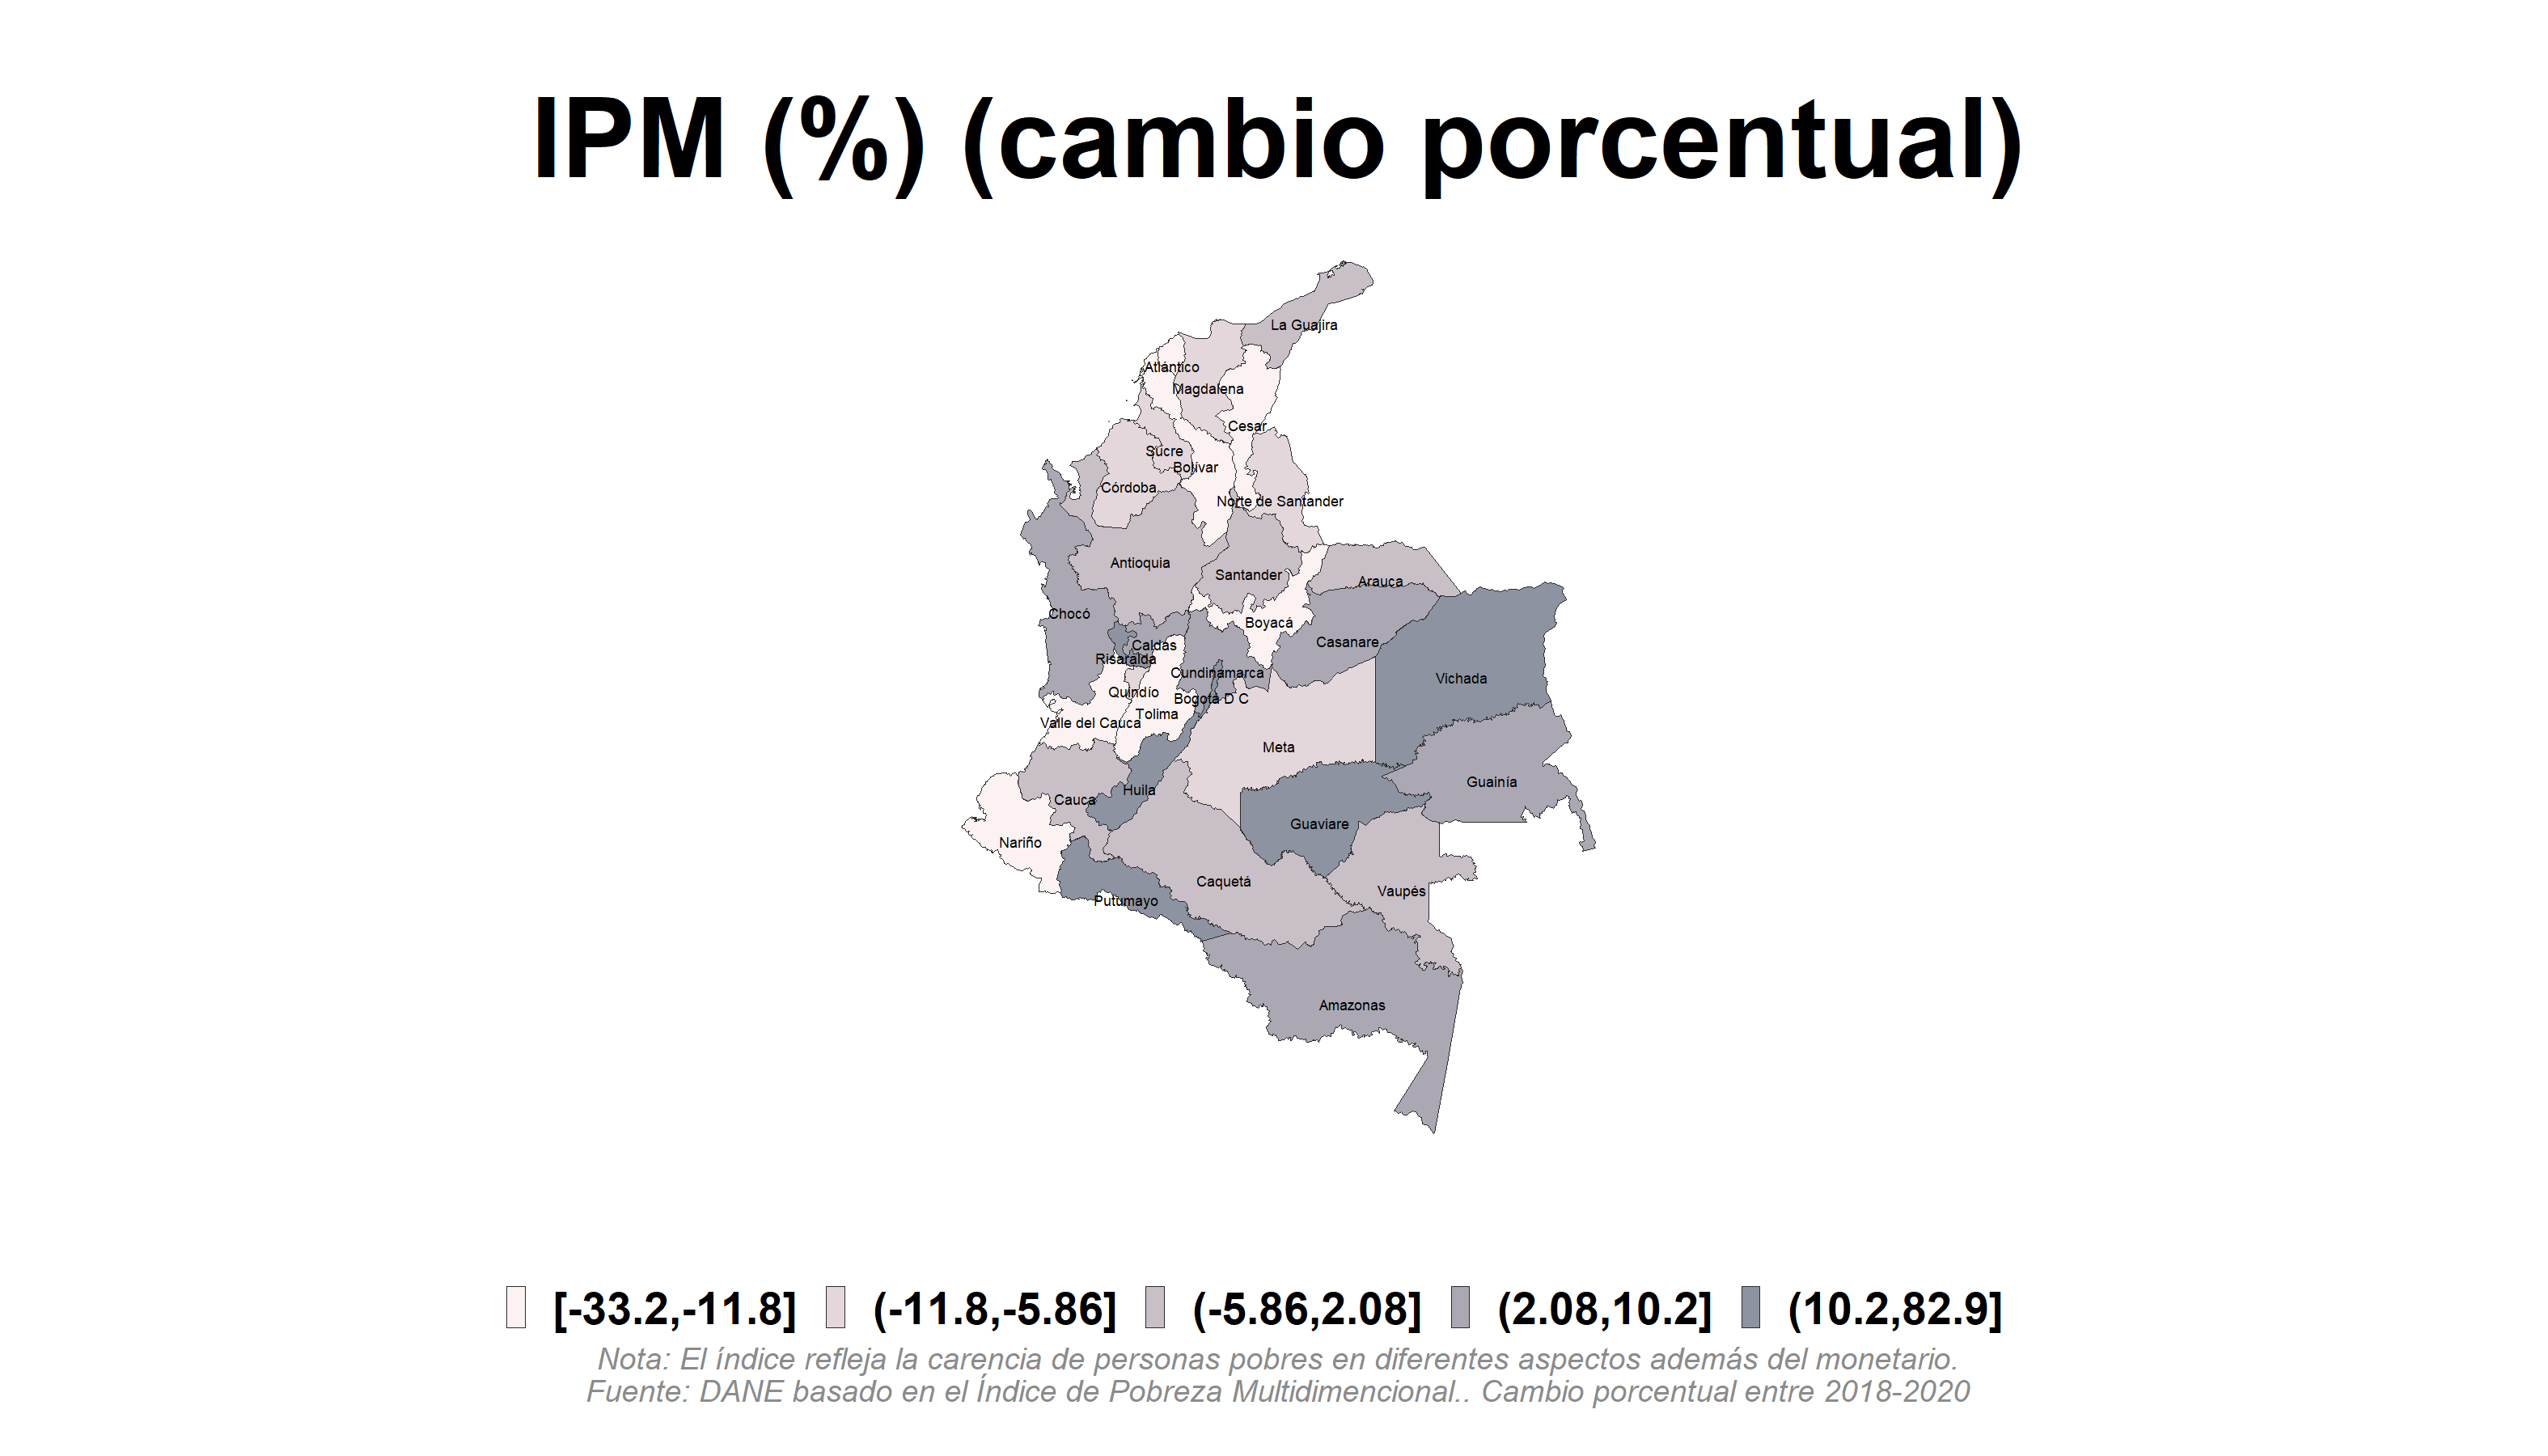
\includegraphics[width=\textwidth,keepaspectratio]{img/var_268_map_change.png}
        \end{center}
    \end{figure}
            \begin{itemize}
                    \item Nariño, Valle, Tolima, Boyacá, Bolívar, Cesar y Atlántico presentan mejoras, disminuyendo más de un 10\% su IPM entre 2018 y 2020.
                    \item Vichada, Guaviare, Putumayo, Huila, Risaralda y Bogotá aumentaron su IPM en más de un 10\% entre los años de referencia.
                    \end{itemize}

%%%% Include figures
    \begin{figure}[H]
        \caption[Índice de Pobreza Multidimensional por departamentos para el 2020 ]{\label{ipm_dptos} }
        \begin{center}
        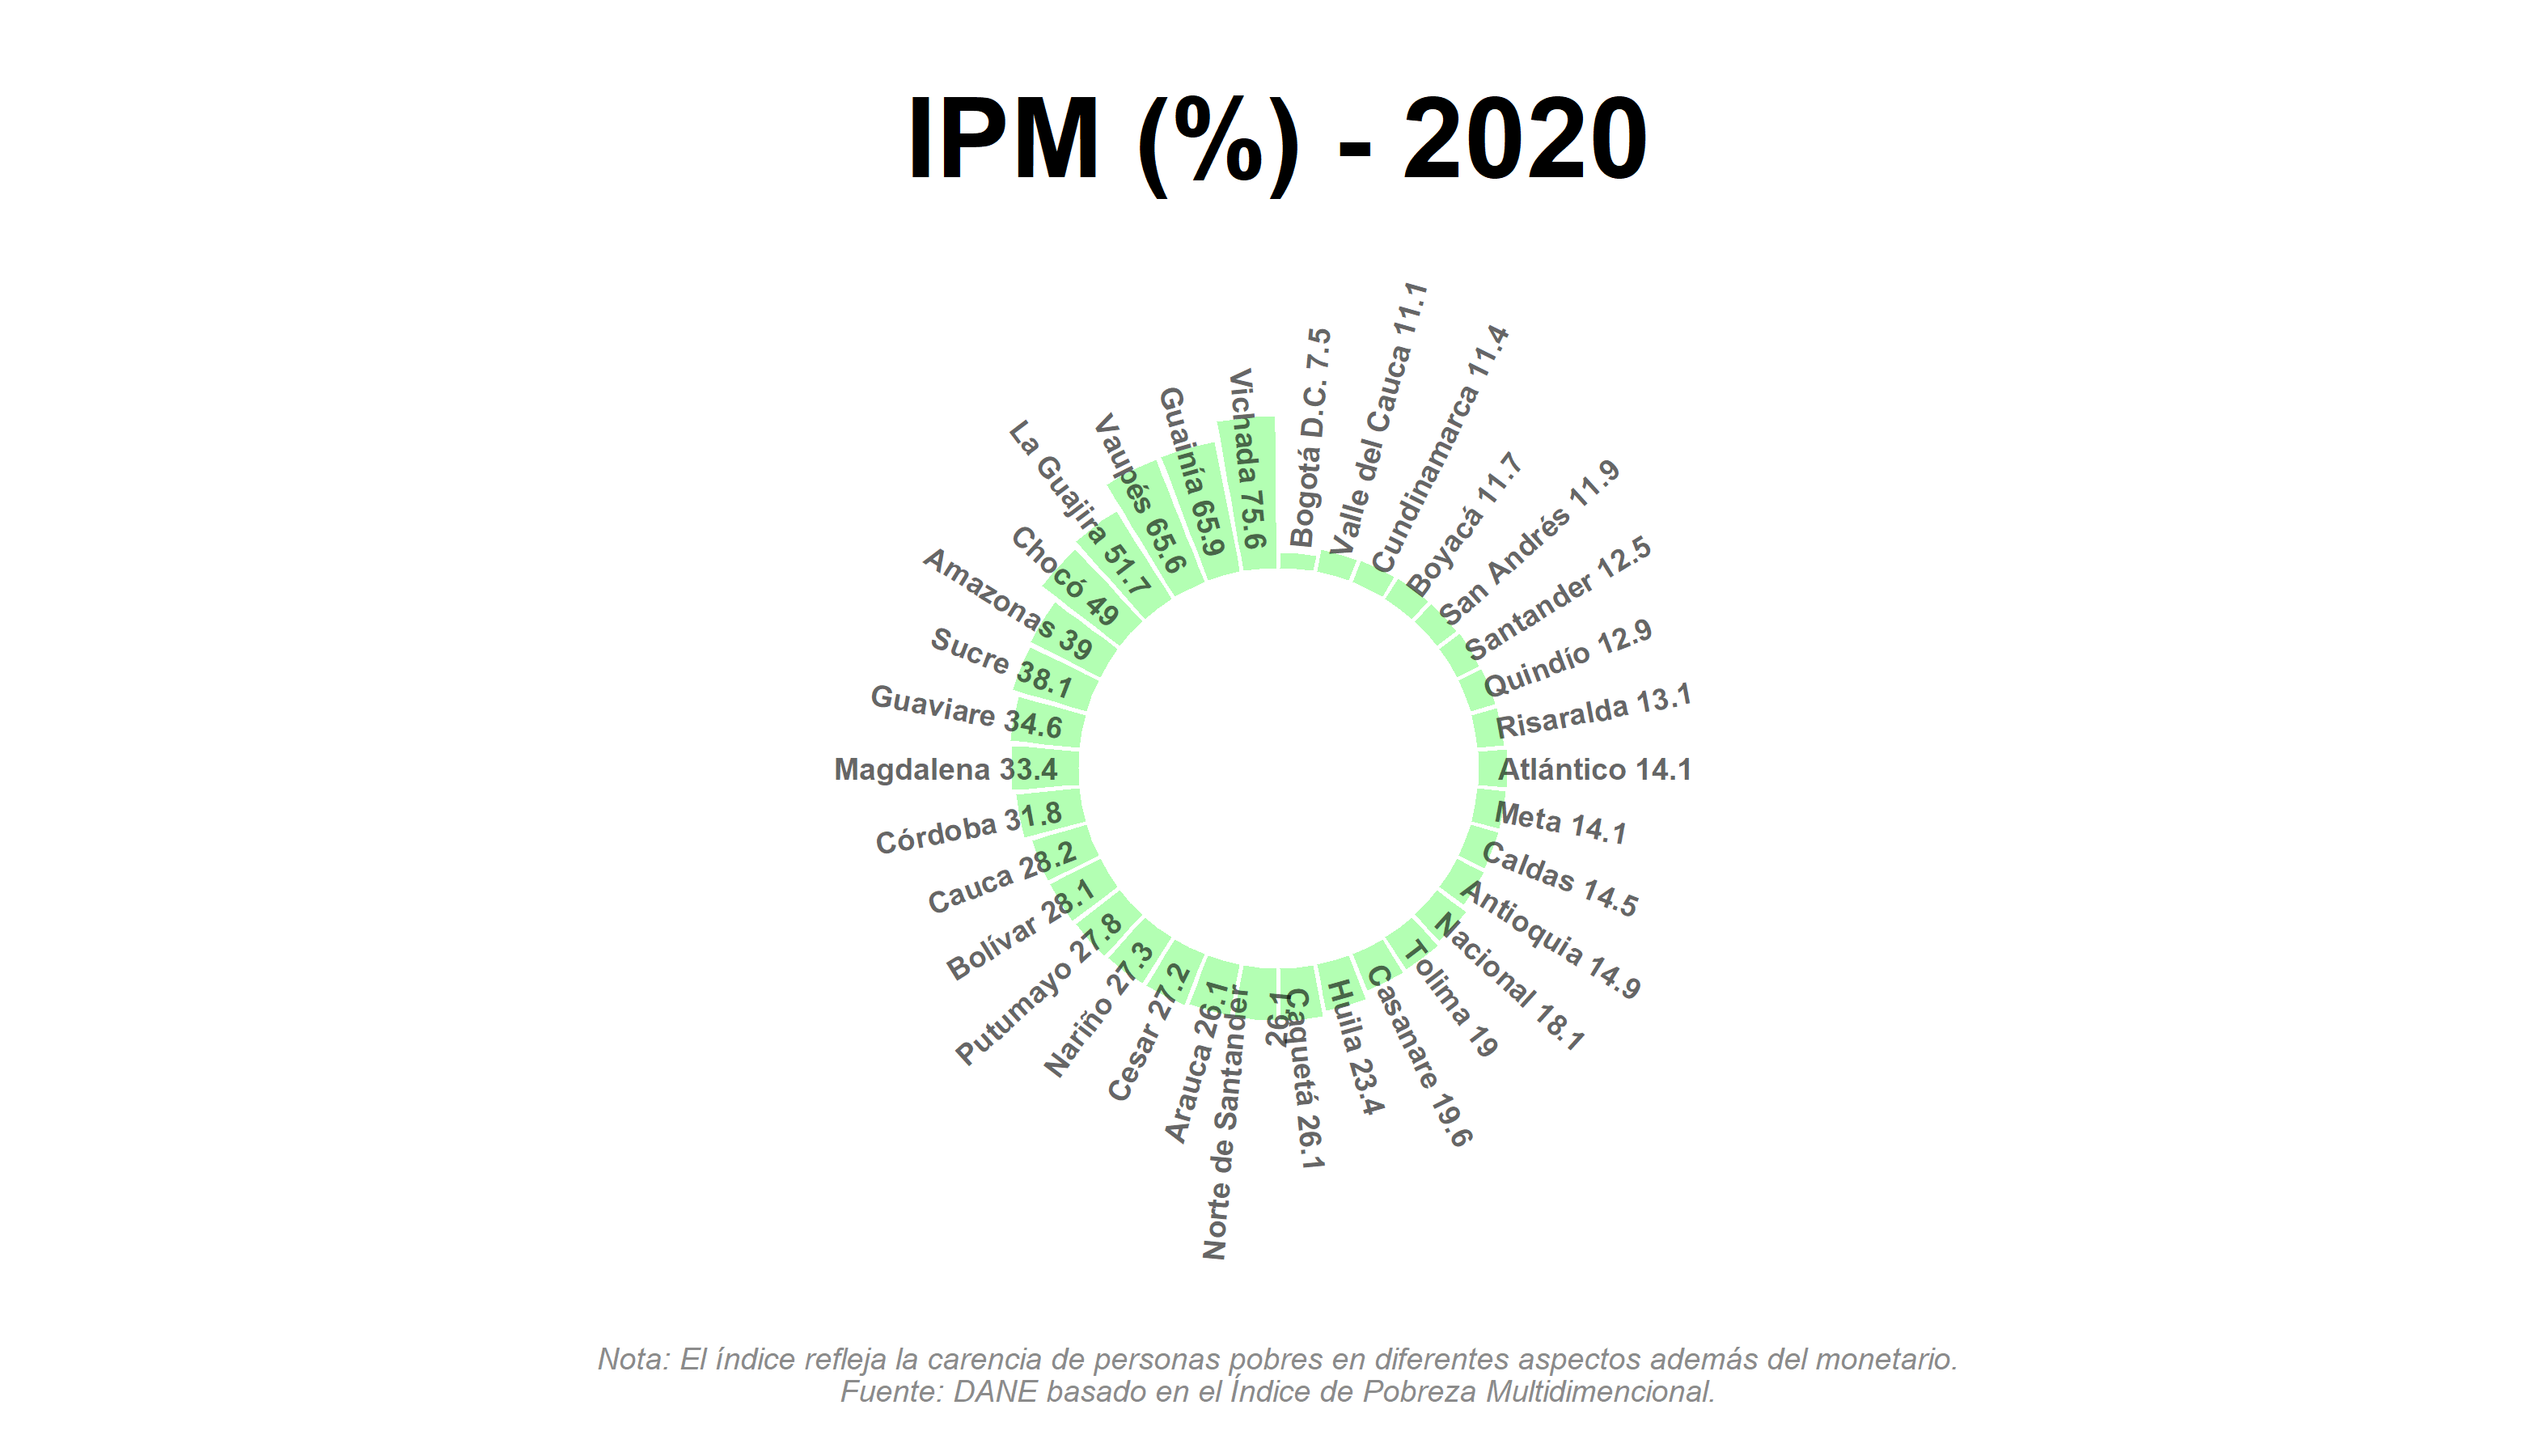
\includegraphics[width=\textwidth,keepaspectratio]{img/var_268_static.png}
        \end{center}
    \end{figure}
            \begin{itemize}
                    \item La distribución del IPM es amplia, desde menos del 10\% hasta por encima del 75\%.
                    \item La diferencia entre los dptos extremos es de aproximadamente un 65\%, teniendo a Bogotá (Distrito capital) con el de menor (7.5\%) y Vichada el de mayor puntaje con un 75.6\%.  
                    \item Hay una diferencia de aproximadamente un 15\% entre los últimos 3 departamentos y el anterior a este, siendo el salto más abrupto en el IPM
                    \end{itemize}

%%%% Include figures
    \begin{figure}[H]
        \caption[Índice de Pobreza Multidimensional por regiones - 2010 VS 2020 ]{\label{ipm_regiones_vs} }
        \begin{center}
        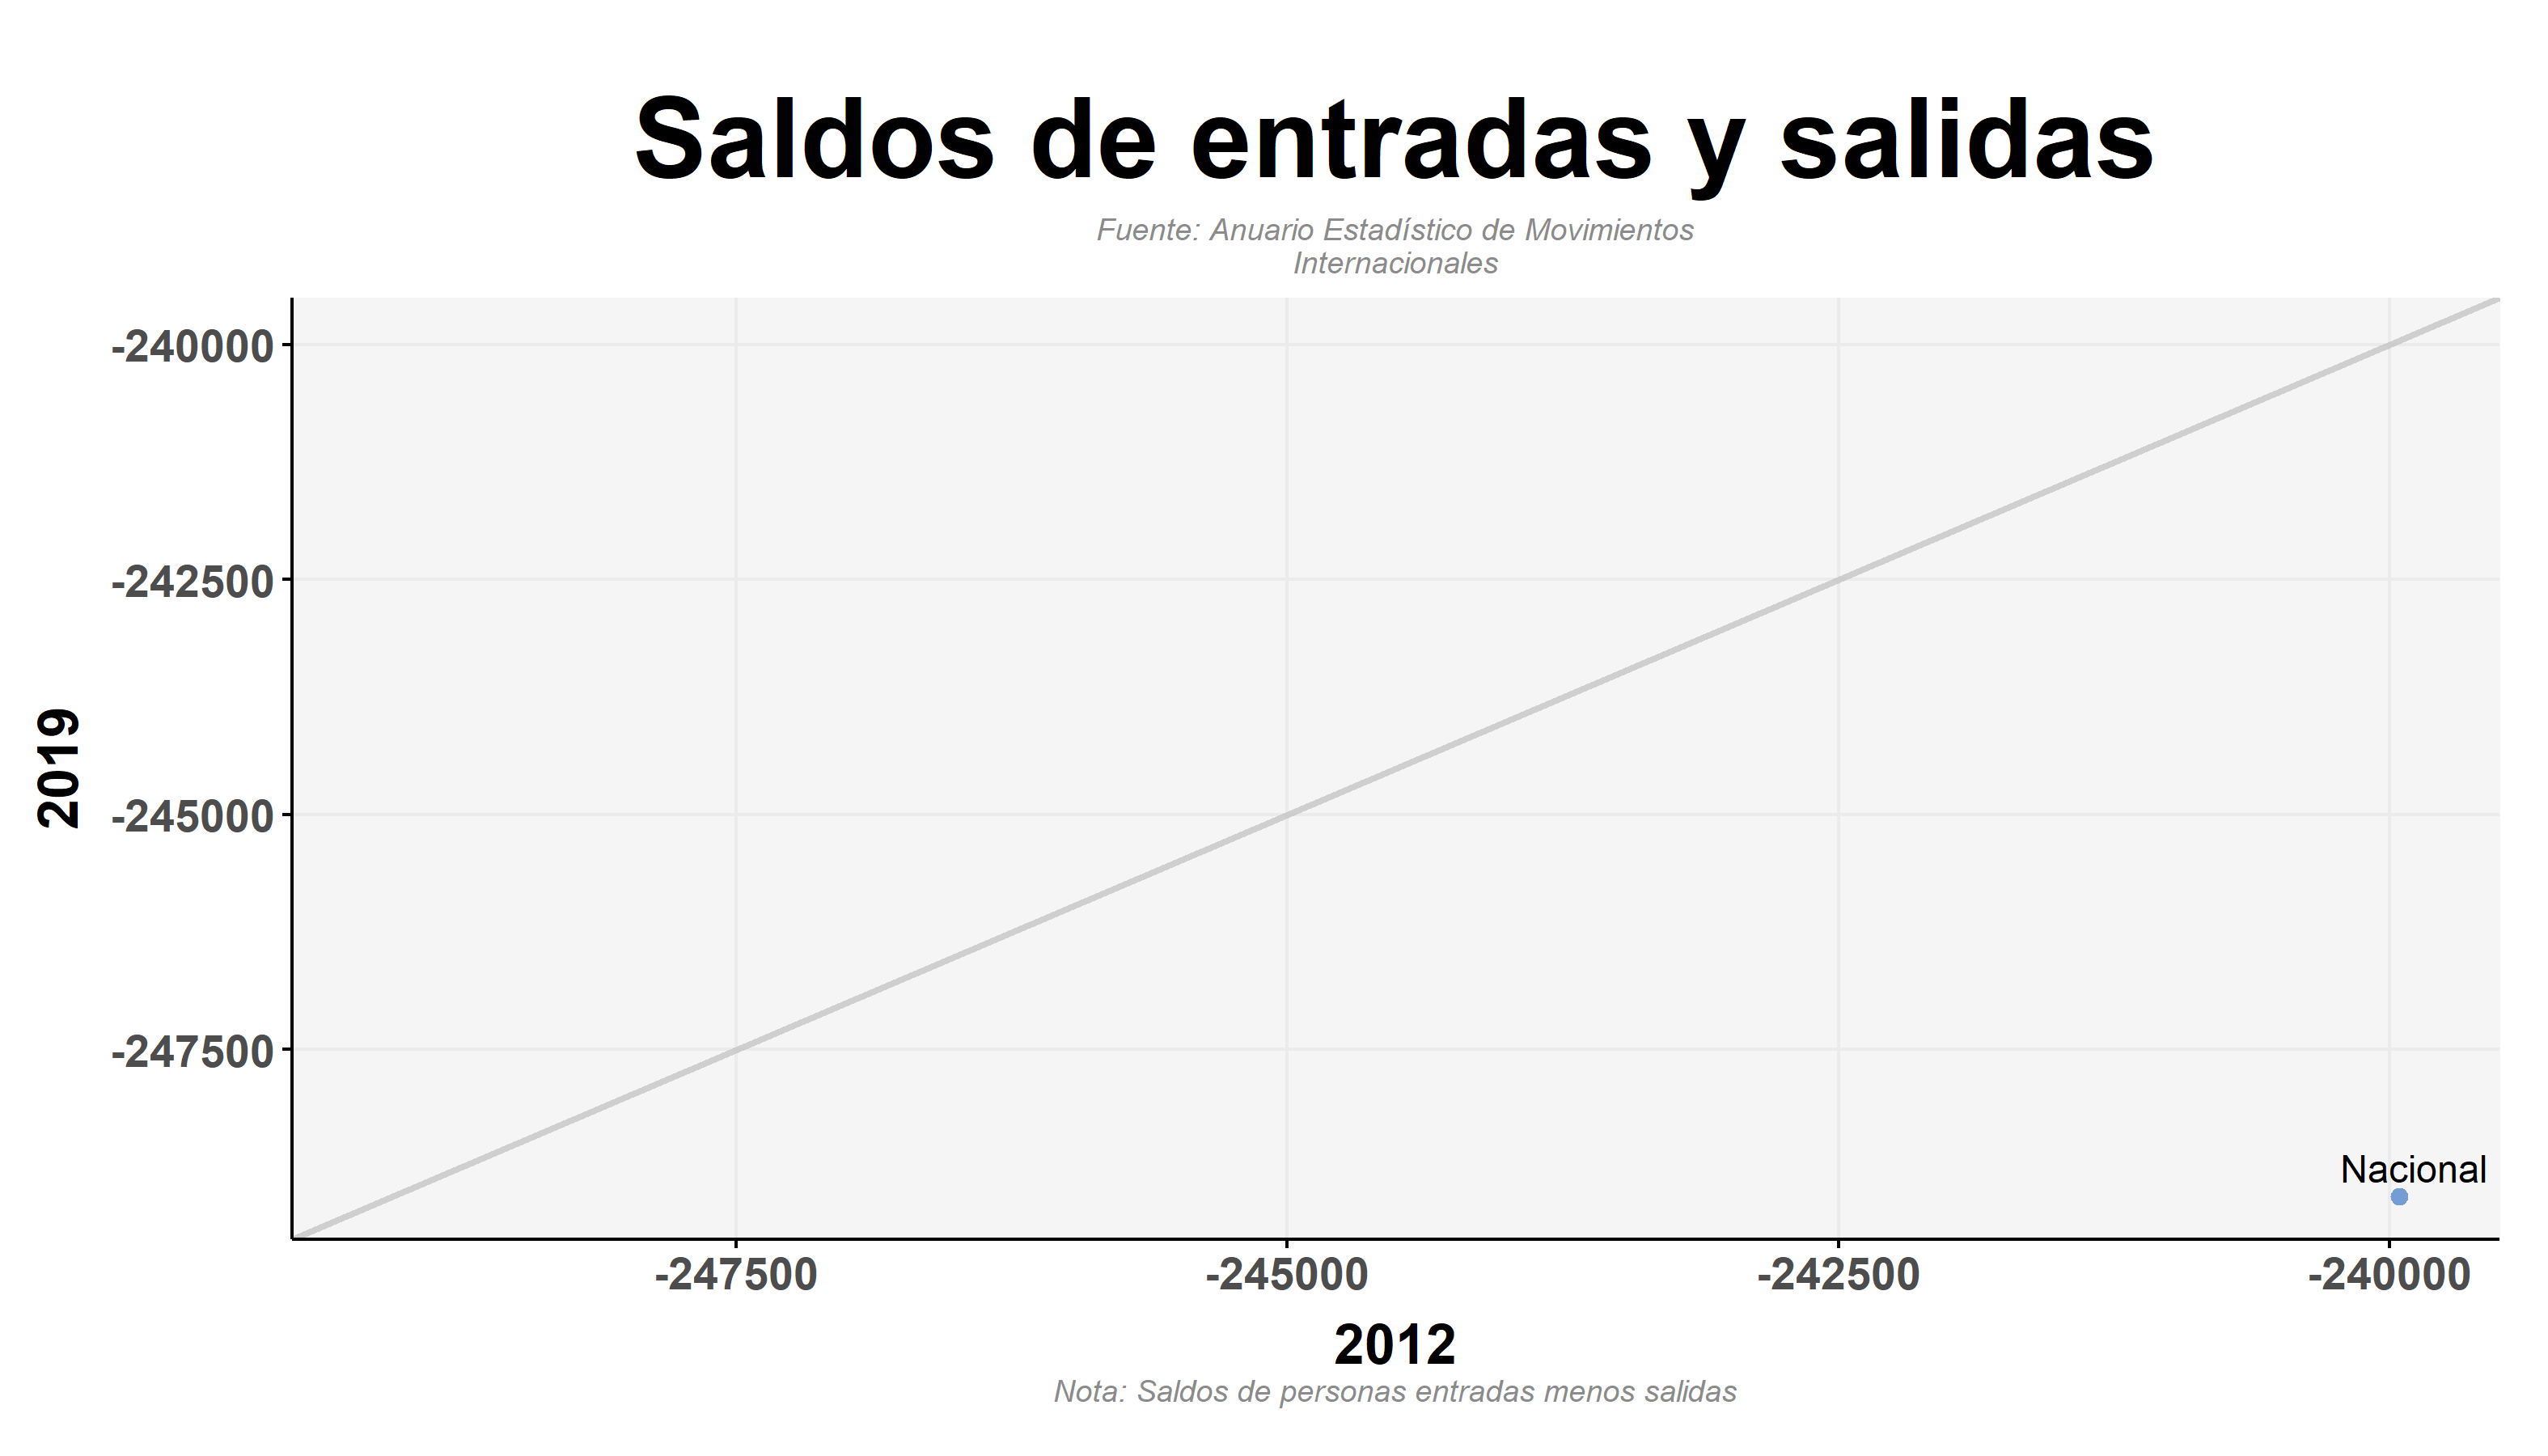
\includegraphics[width=\textwidth,keepaspectratio]{img/var_270_scatter_time.png}
        \end{center}
    \end{figure}
            \begin{itemize}
                    \item Todas las regiones tuvieron resultados menores en para 2020 comparados con los del 2012.
                    \item La distribución de puestos no cambio a excepción de los dos primeros (IPM más altos) donde la región Pacífica pasó de ser segundo a reemplazar a la Caribe que estaba de primero en el 2012.
                    \item La región Caribe es la que presenta una mayor mejoría, aproximadamente un 15\%.
                    \end{itemize}

%%%% Include figures
    \begin{figure}[H]
        \caption[Índice de Pobreza Multidimensional por zonas y nacional ]{\label{ipm_zonas} }
        \begin{center}
        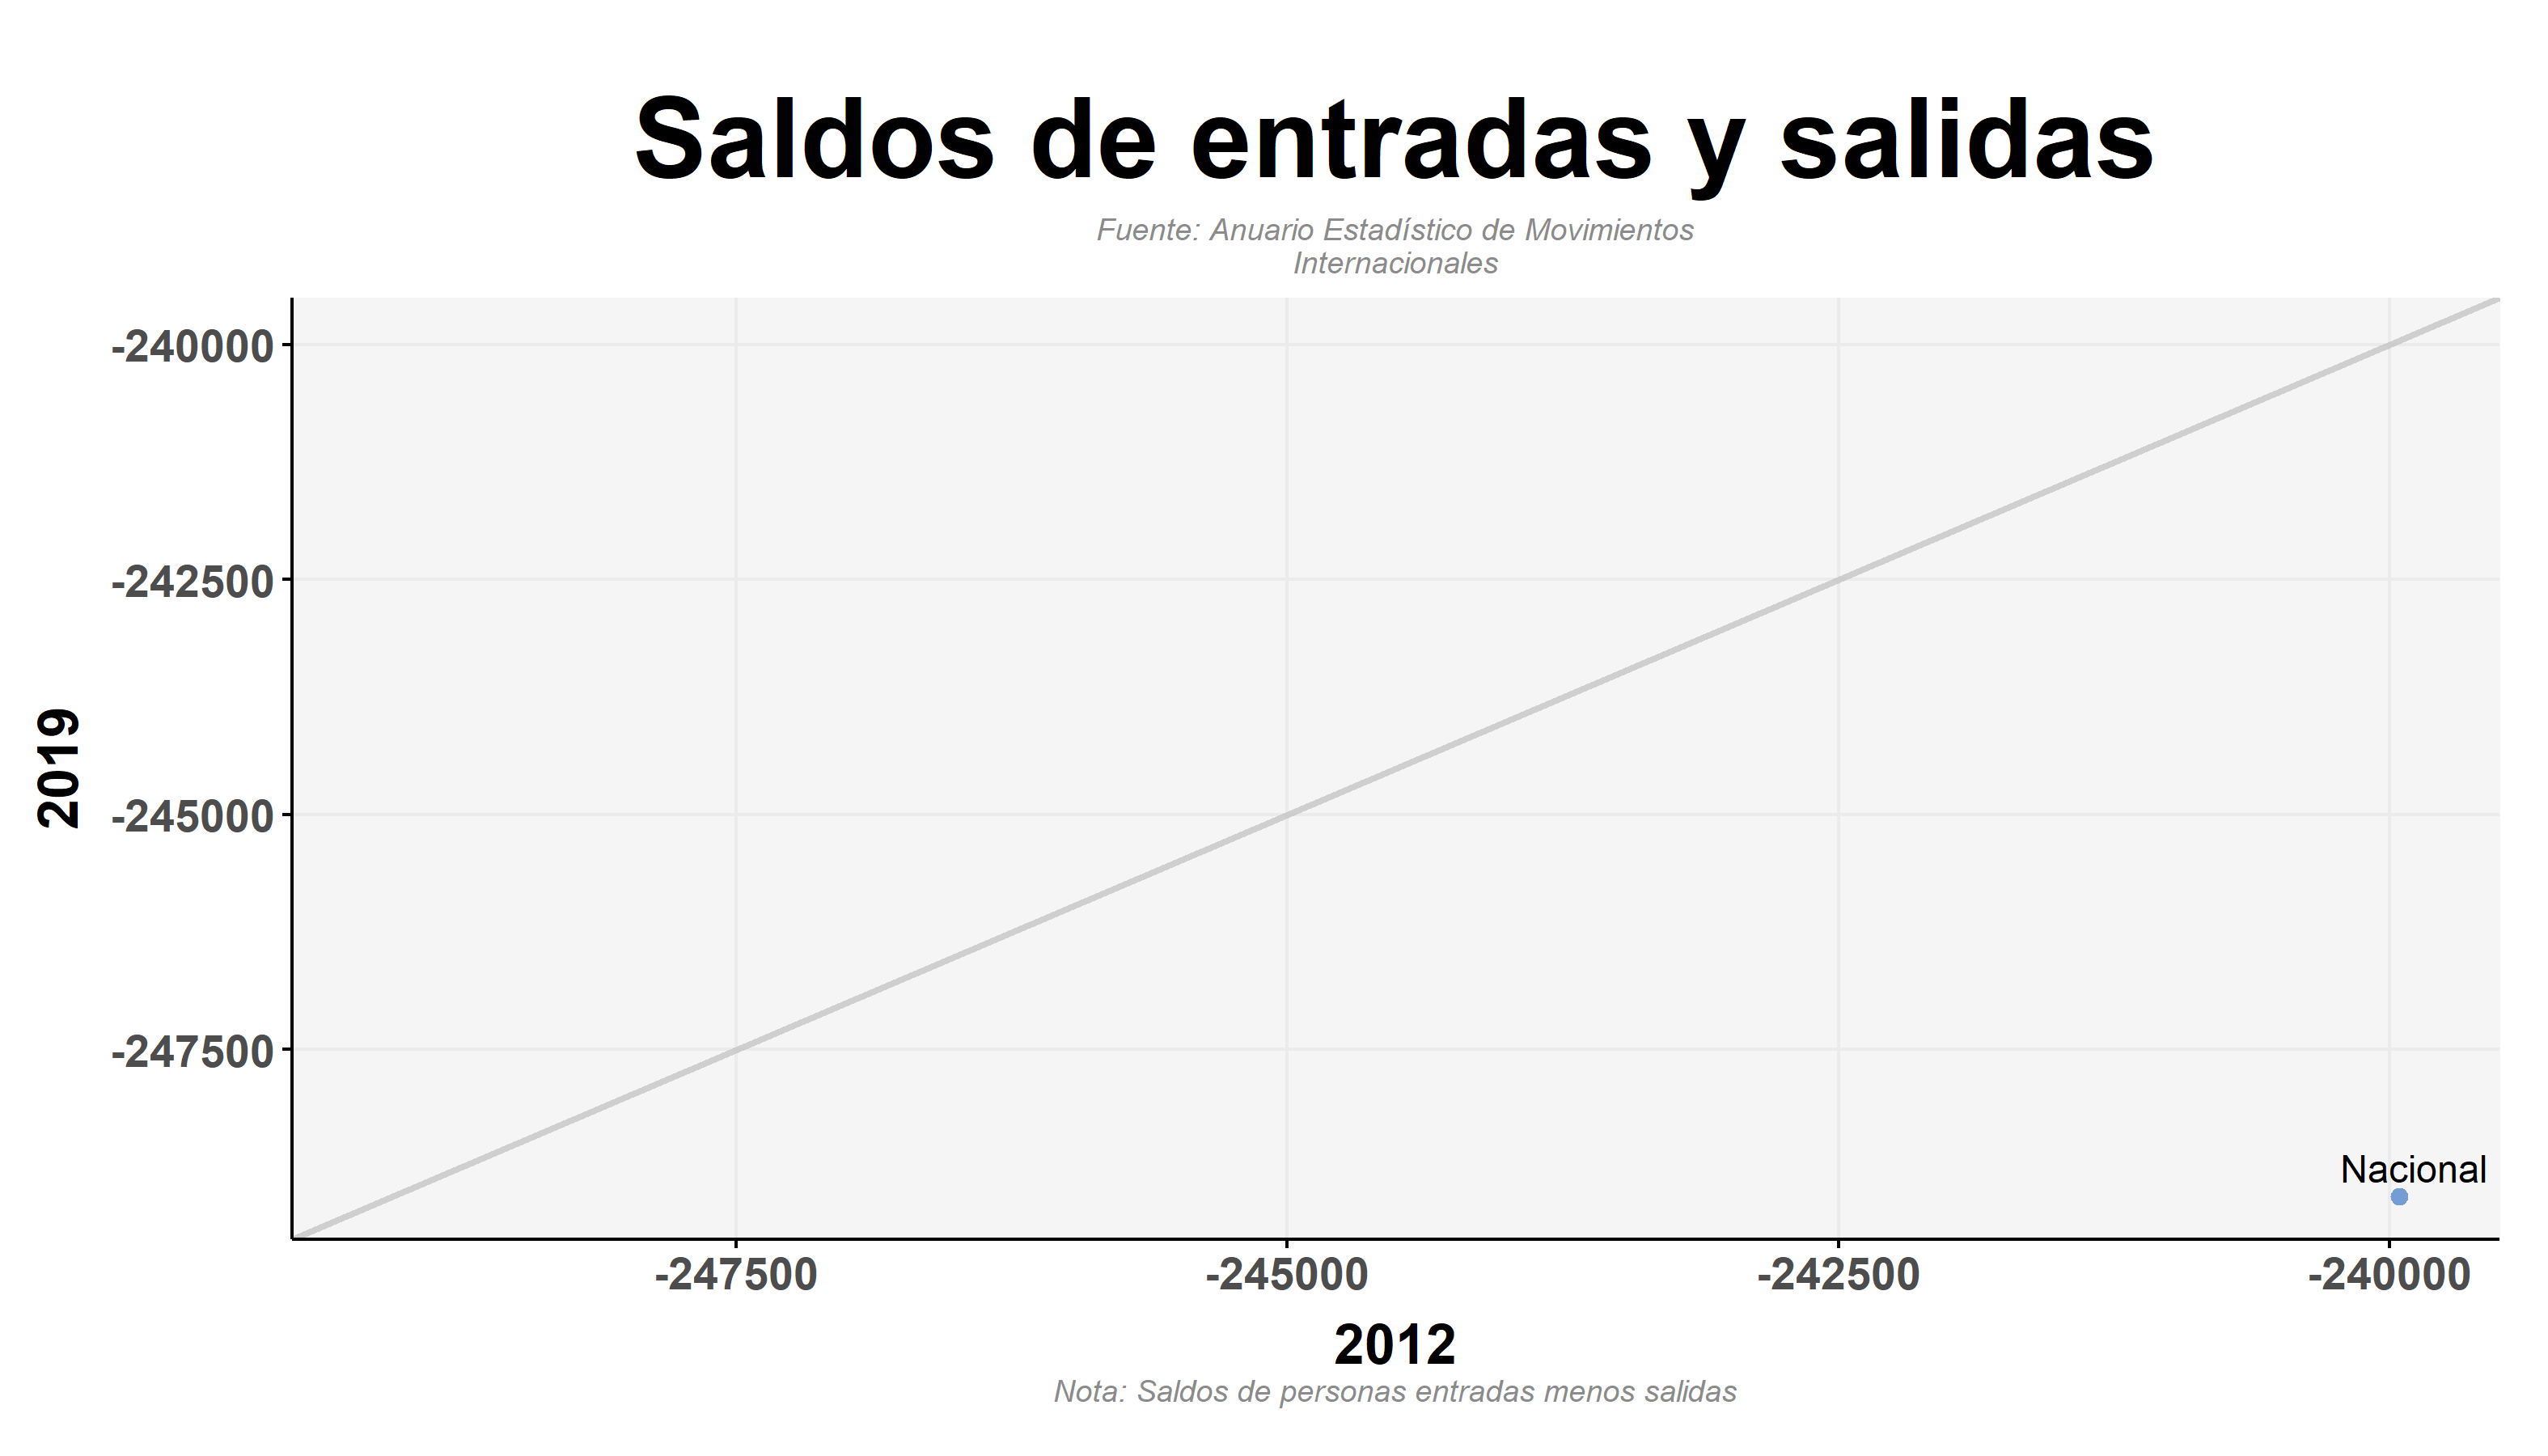
\includegraphics[width=\textwidth,keepaspectratio]{img/var_270_scatter_time.png}
        \end{center}
    \end{figure}
            \begin{itemize}
                    \item El IPM en general vemos que para las cabeceras y nacional han estado bajando y desde el 2017 se han subido los niveles levemente hasta el pico en el 2018, donde baja para 2019 y hay un leve aumento en 2020.
                    \item A nivel de centros poblados y rural vemos que a pesar de tener el mismo comportamiento sus cambios son más abruptos, como el pico de 2018 que se denota que viene aumentando después del 2016 y el del 2020 que aparece como un retroceso de la mitad de lo que disminuyó en 2019.
                    \item Para el 2020 se registraron IPM menores que los registrados en 2010, lo que demuestra una mejora en los últimos 10 años.
                    \item La zona rural parece más sensible a los cambios en términos del IPM.
                    \end{itemize}

        \subsubsection{Necesidades Básicas Insatisfechas - NBI}
        
%%%% Include figures
    \begin{figure}[H]
        \caption[Necesidades Básicas Insatisfechas - Minorías VS no minorías ]{\label{nbi_minorias_vs} }
        \begin{center}
        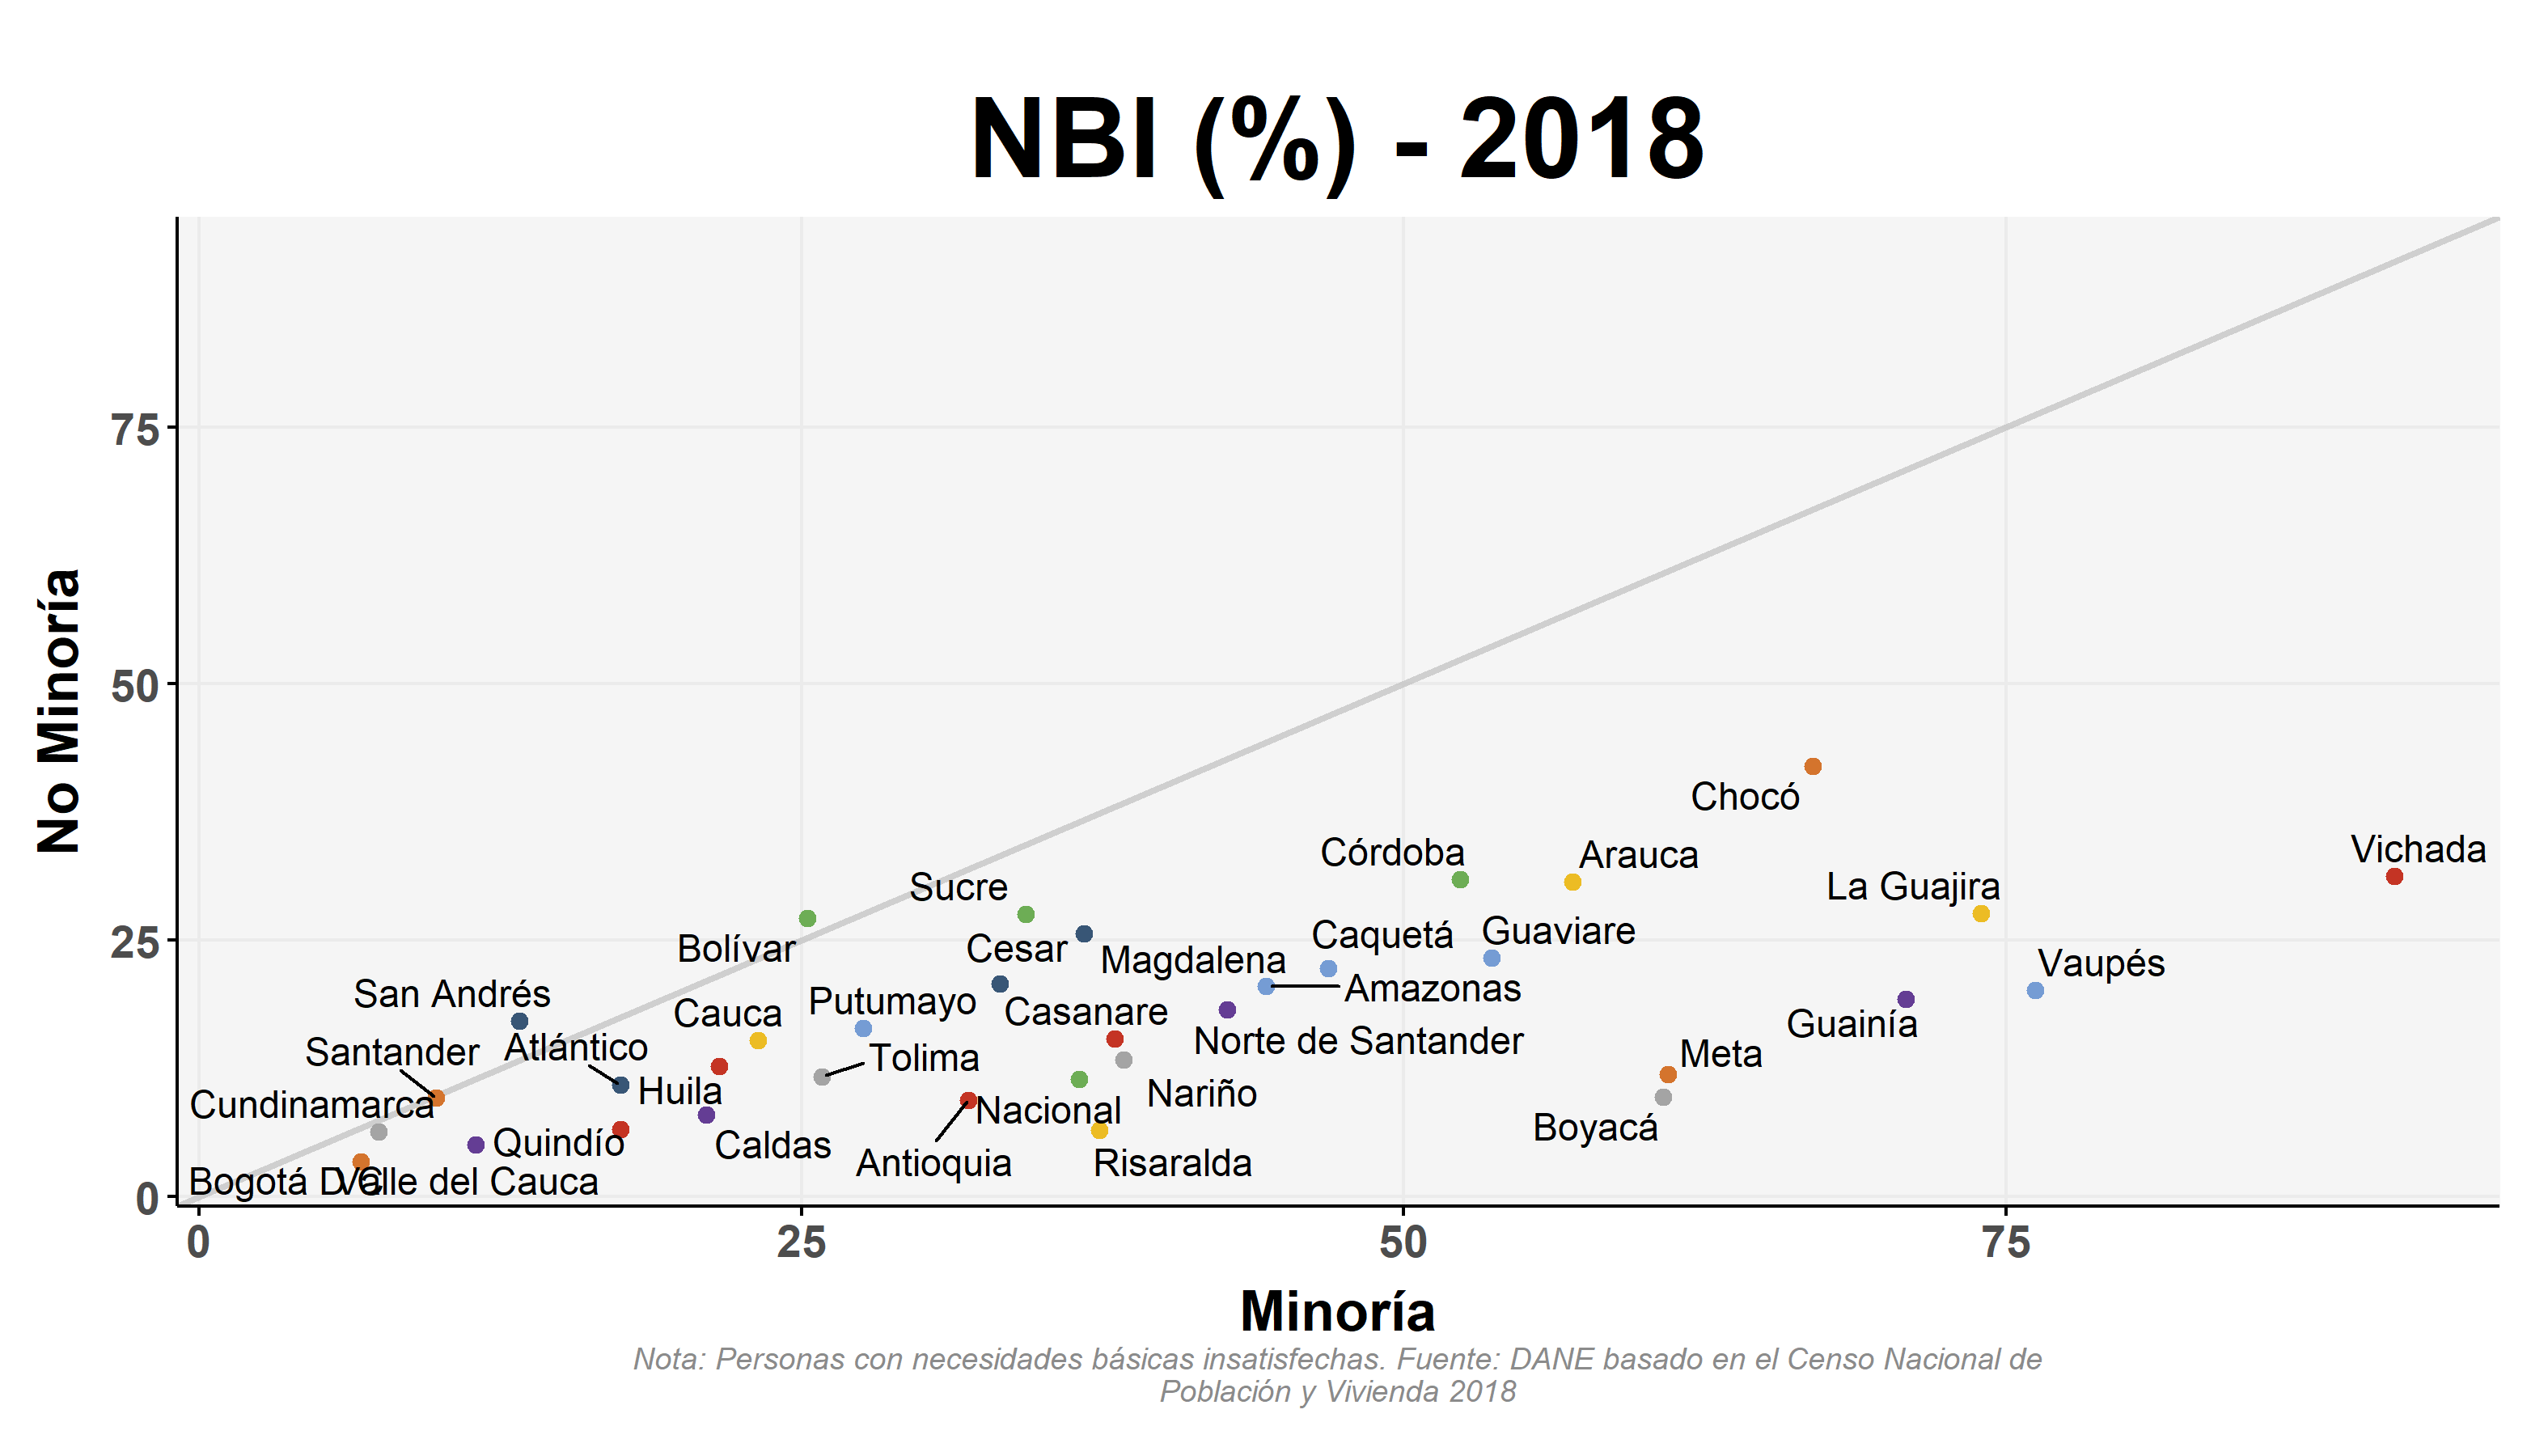
\includegraphics[width=\textwidth,keepaspectratio]{img/var_272_scatter.png}
        \end{center}
    \end{figure}
            \begin{itemize}
                    \item Gran parte de los departamentos tienen NBI de las no minorías por debajo del 30\%, mientras que las de las minorías están distribuidas entre 0 y 75\%. 
                    \item Solo San Andrés y Bolívar presentan NBI mayores para las no minorías que para las minorías.
                    \item Cundinamarca y Santander presentan valores similares de NBI entre minorías y no minorías.
                    \item A nivel nacional encontramos que las minorías tienen NBI por encima del 35\% mientras que las no minorías están cerca del 10\%, con una diferencias de más del 20\%.
                    \end{itemize}

%%%% Include figures
    \begin{figure}[H]
        \caption[Necesidades Básicas Insatisfechas para minorías y no minorías en el 2018 ]{\label{nbi_minorias} }
        \begin{center}
        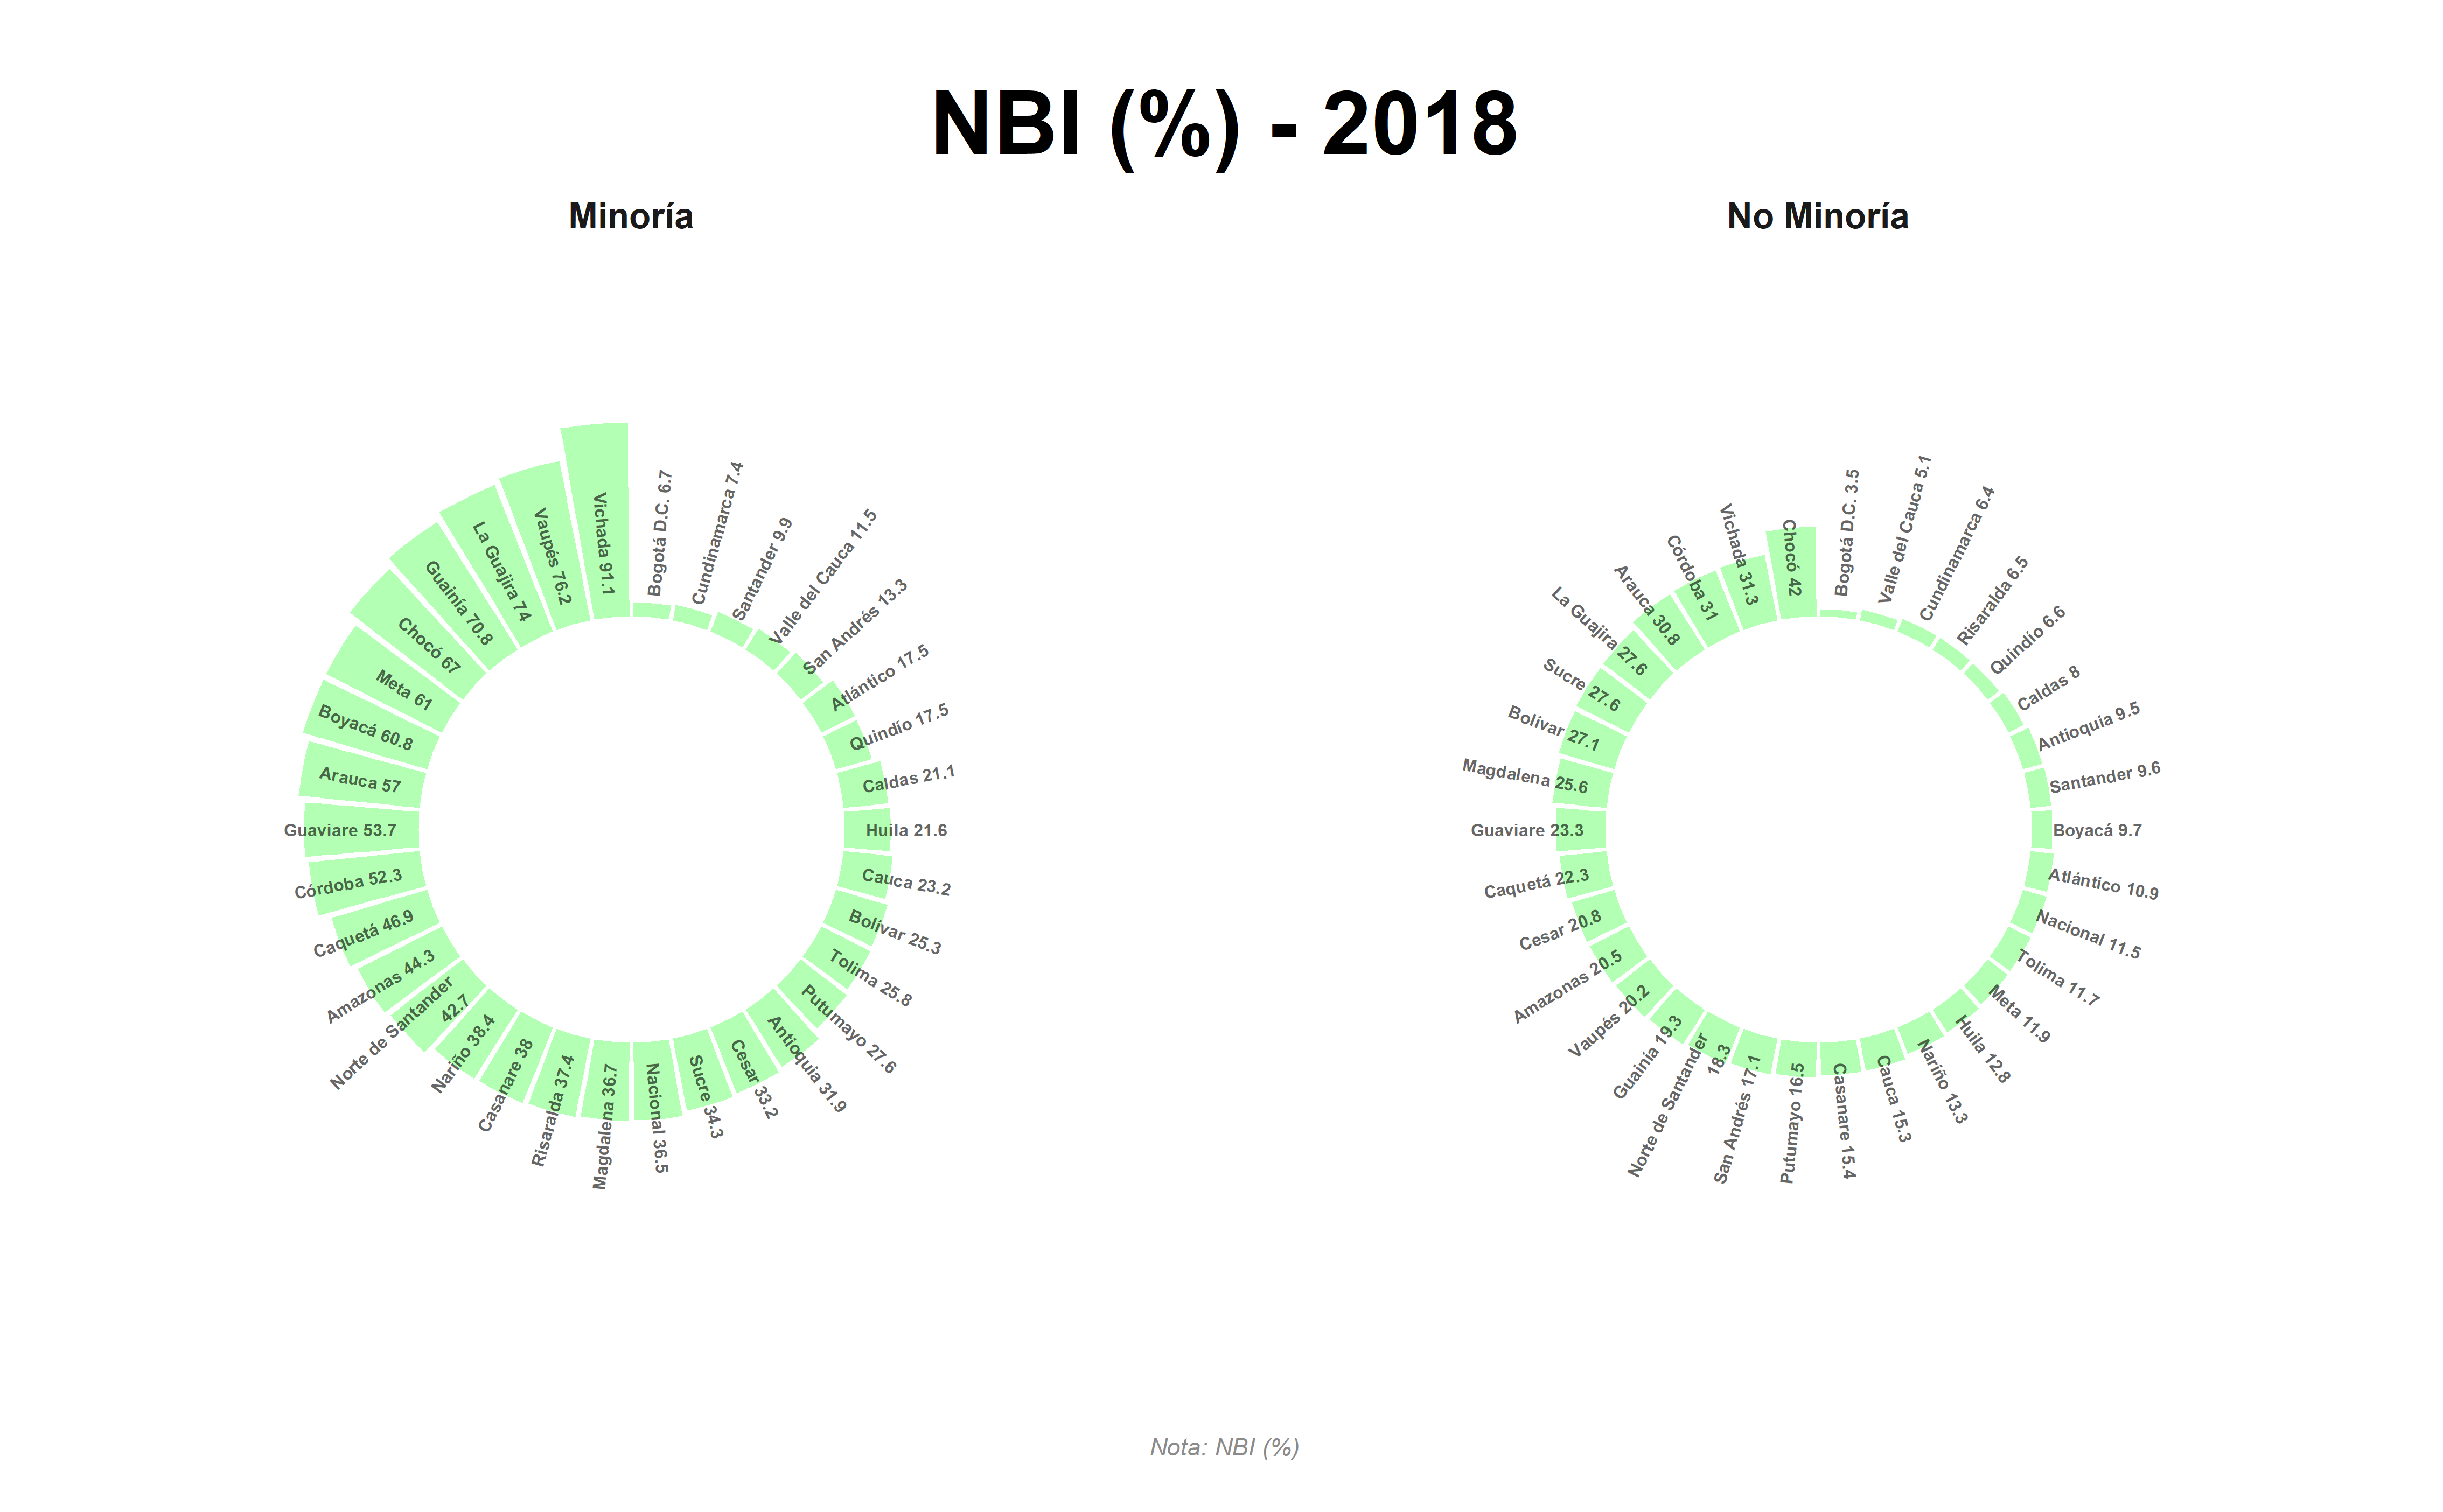
\includegraphics[width=\textwidth,keepaspectratio]{img/var_272_static.png}
        \end{center}
    \end{figure}
            \begin{itemize}
                    \item Bogotá es la zona con menor nivel de NBI para ambos, mientras que Vichada es el de mayor para las minorías y Chocó para las no minorías.
                    \item La diferencia entre las zonas extremos es de poco menos del 40\% para las no minorías (Bogotá - Chocó) y de más del 80\% para las minorías (Bogotá - Vichada).
                    \item La distribución de NBI es menor para las no minorías (3 a 42\%), teniendo un salto del 10\% aproximadamente entre el último y el anterior a este, mientras que las minorías tienen una mayor área de distribución (6 a 92\%) con un salto de aproximadamente 15\% entre los dos últimos.
                    \end{itemize}

%%%% Include figures
    \begin{figure}[H]
        \caption[Necesidades Básicas Insatisfechas por departamentos para el 2018 (mapa) ]{\label{nbi_dptos_mapa} }
        \begin{center}
        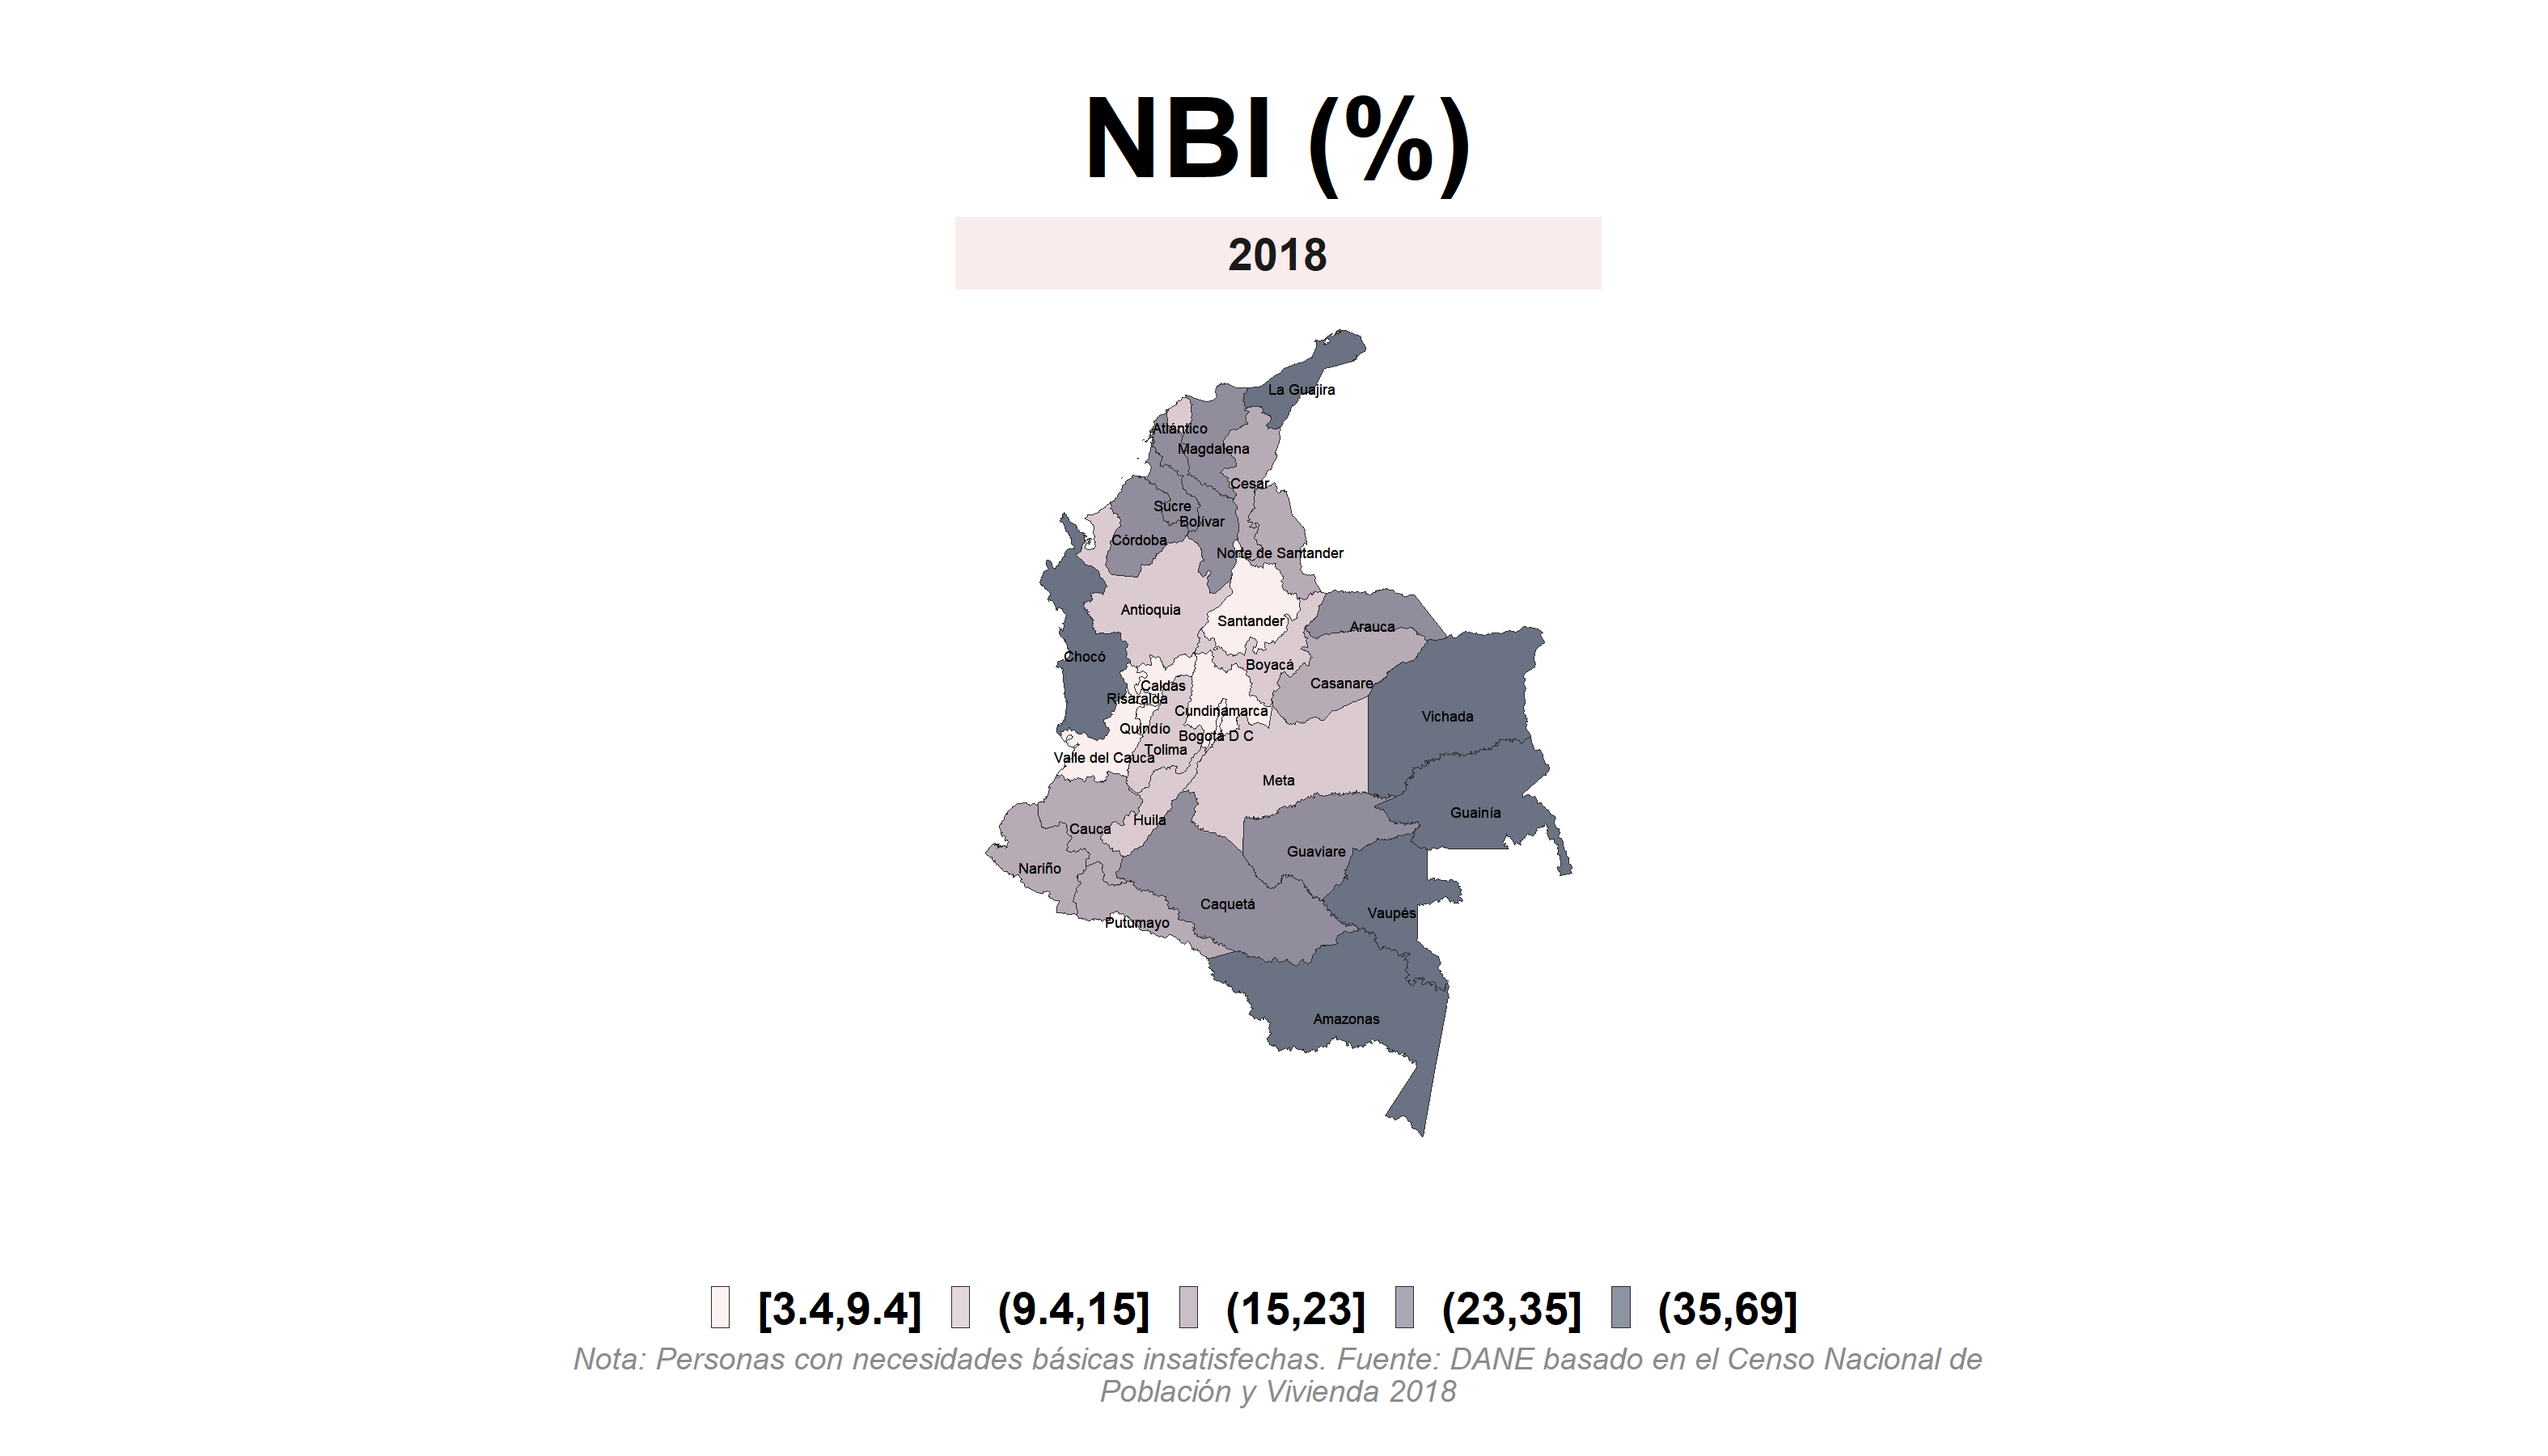
\includegraphics[width=\textwidth,keepaspectratio]{img/var_273_map.png}
        \end{center}
    \end{figure}
            \begin{itemize}
                    \item Valle, Quindío, Risaralda, Caldas, Cundinamarca, Bogotá y Santander son los departamentos con menor porcentaje de NBI, menos del 10\%.
                    \item Se ve que hacia el centro del país se encuentran los departamentos con menores niveles de NBI, mientras que a la periferia se ve como aumentan estas.
                    \item Vichada, Guainía, Vaupés, Amazonas, Chocó y La Guajira tienen el mayor porcentaje de NBI, por encima de 35\%. Todos los departamentos están en la frontera del país, siendo gran parte de estos en los llanos orientales y la Amazonia.
                    \end{itemize}

%%%% Include figures
    \begin{figure}[H]
        \caption[Necesidades Básicas Insatisfechas por departamentos para 2018 ]{\label{nbi_dptos} }
        \begin{center}
        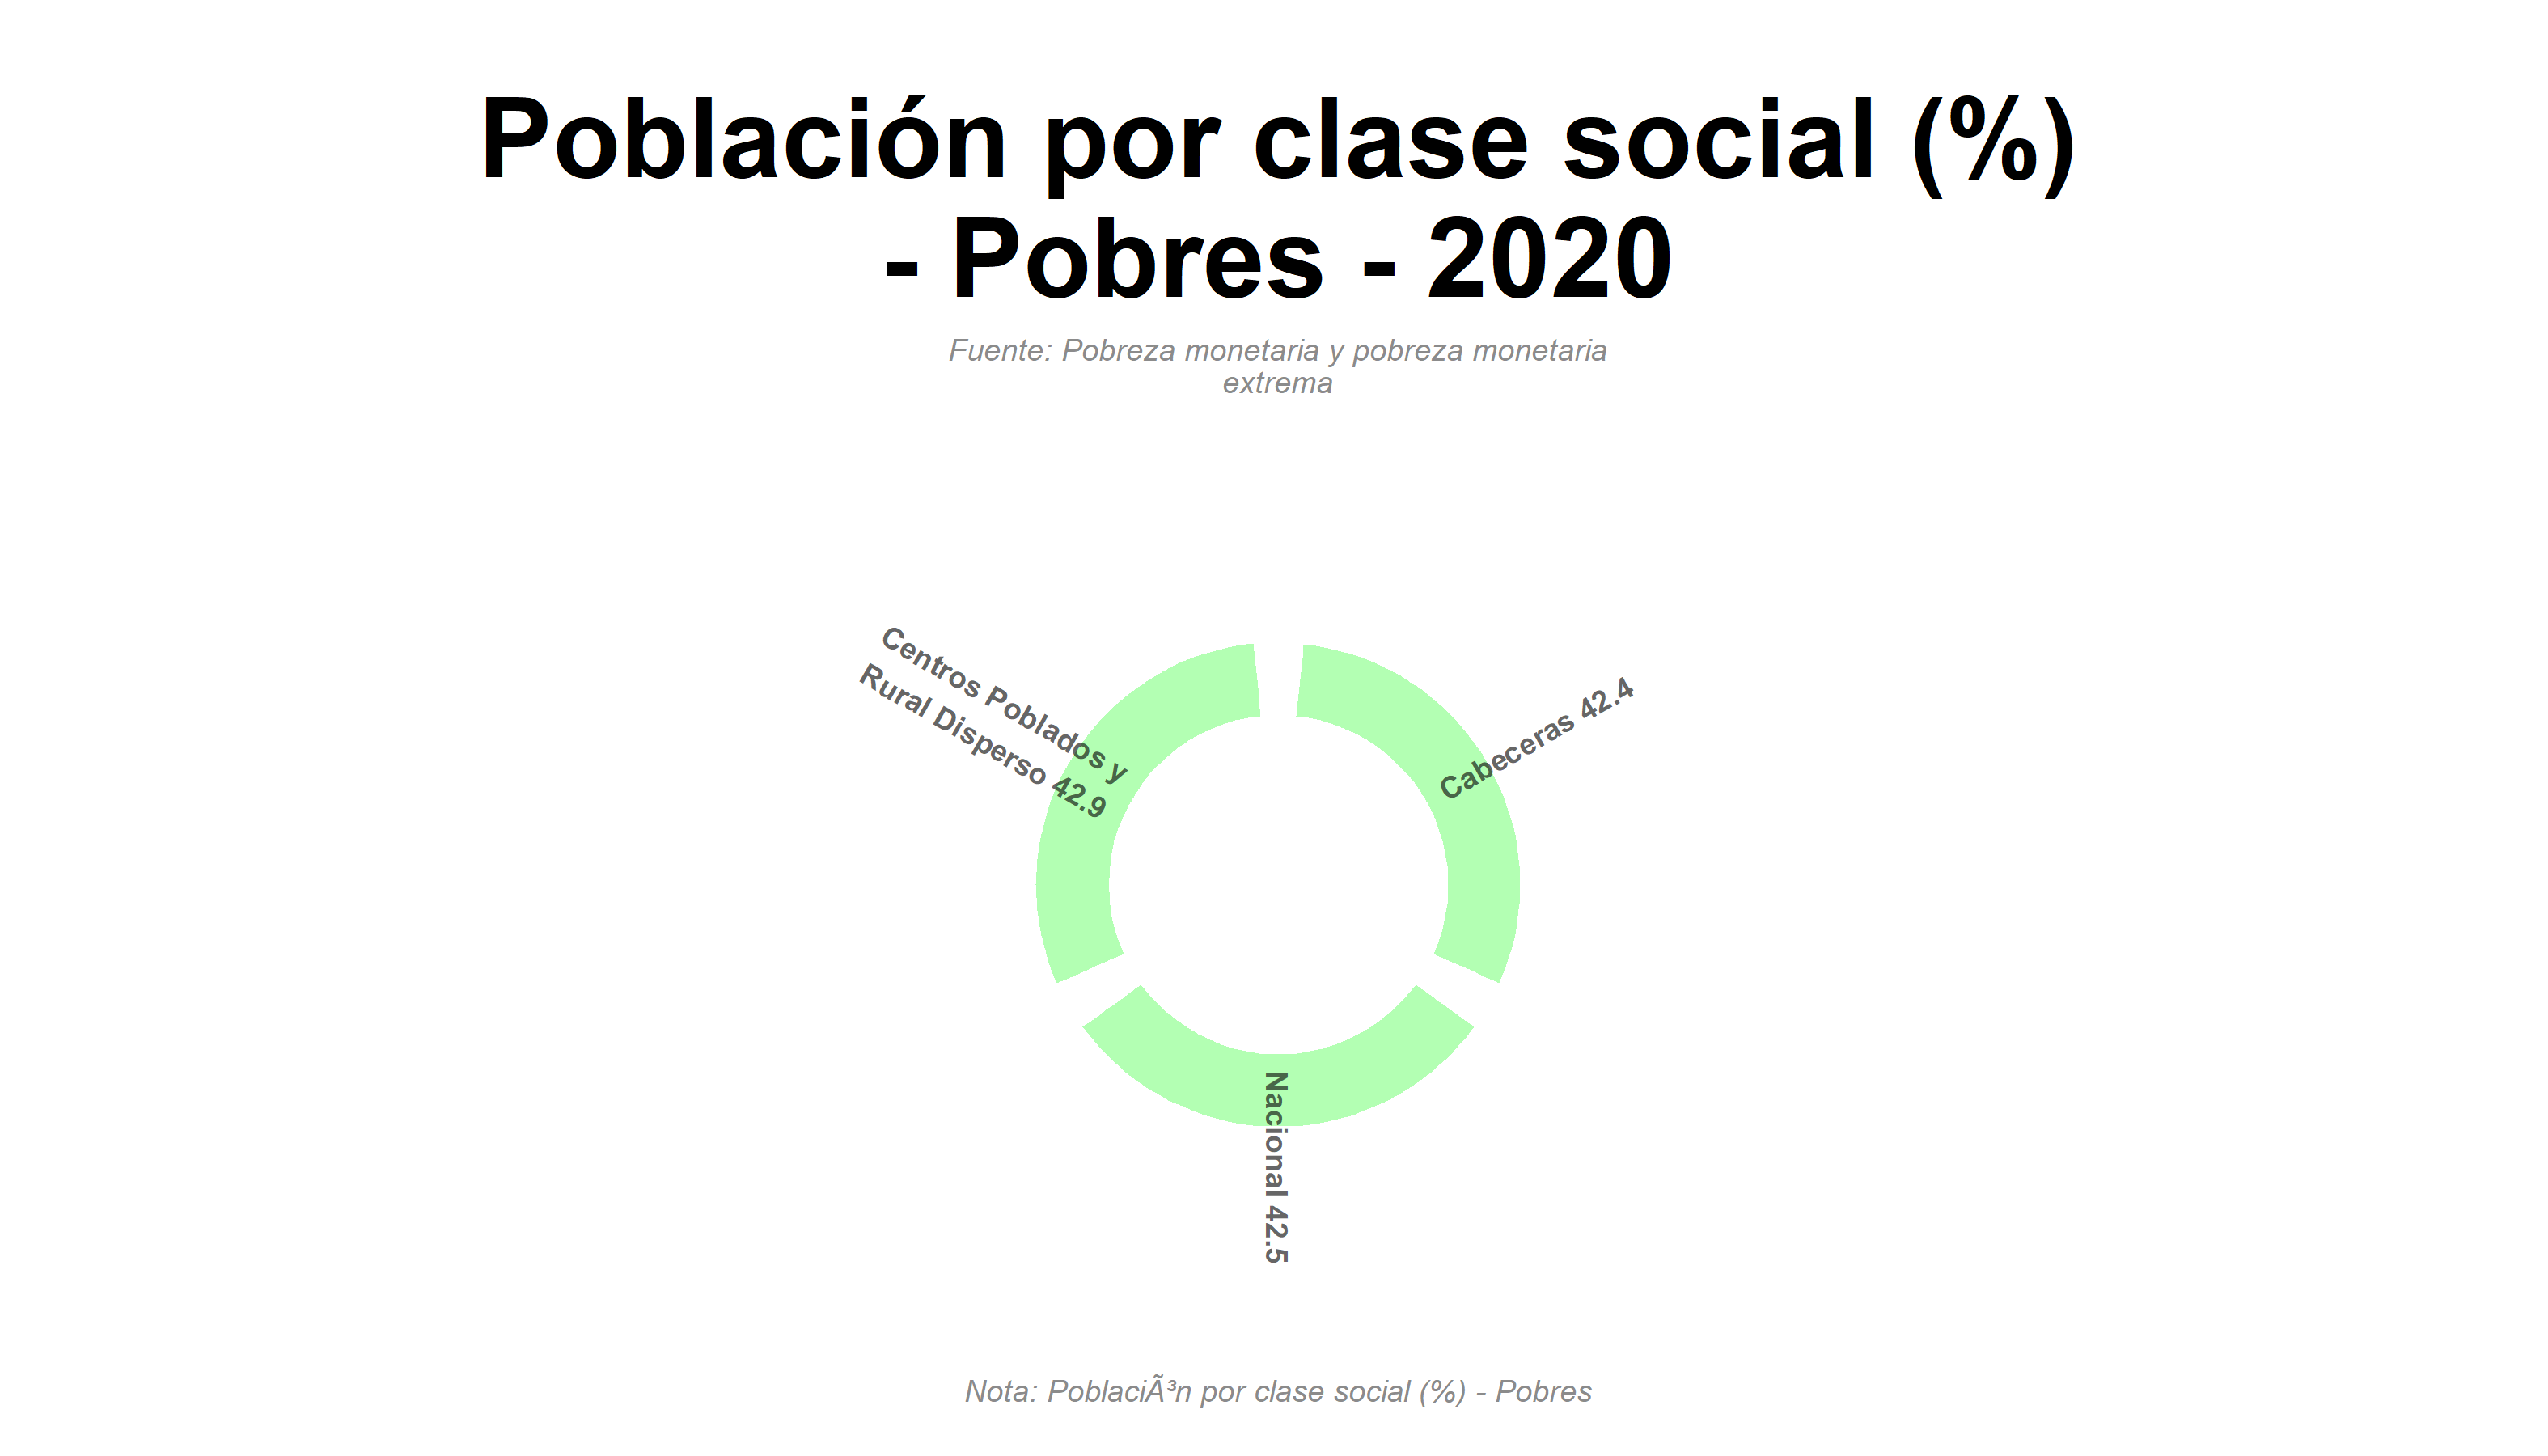
\includegraphics[width=\textwidth,keepaspectratio]{img/var_273_static.png}
        \end{center}
    \end{figure}
            \begin{itemize}
                    \item La distribución de las NBI está en gran parte de los dptos entre 3 y 35\%, y los últimos 5 dptos entre 50 y 69\%, siendo un salto de poco más del 15\% entre estos y el anterior a estos.
                    \item La diferencia entre las zonas extremo es de aproximadamente un 65\% (Bogotá - Vaupés)
                    \end{itemize}

%%%% Include figures
    \begin{figure}[H]
        \caption[Necesidades Básicas Insatisfechas por zonas y nacional ]{\label{nbi_zonas} }
        \begin{center}
        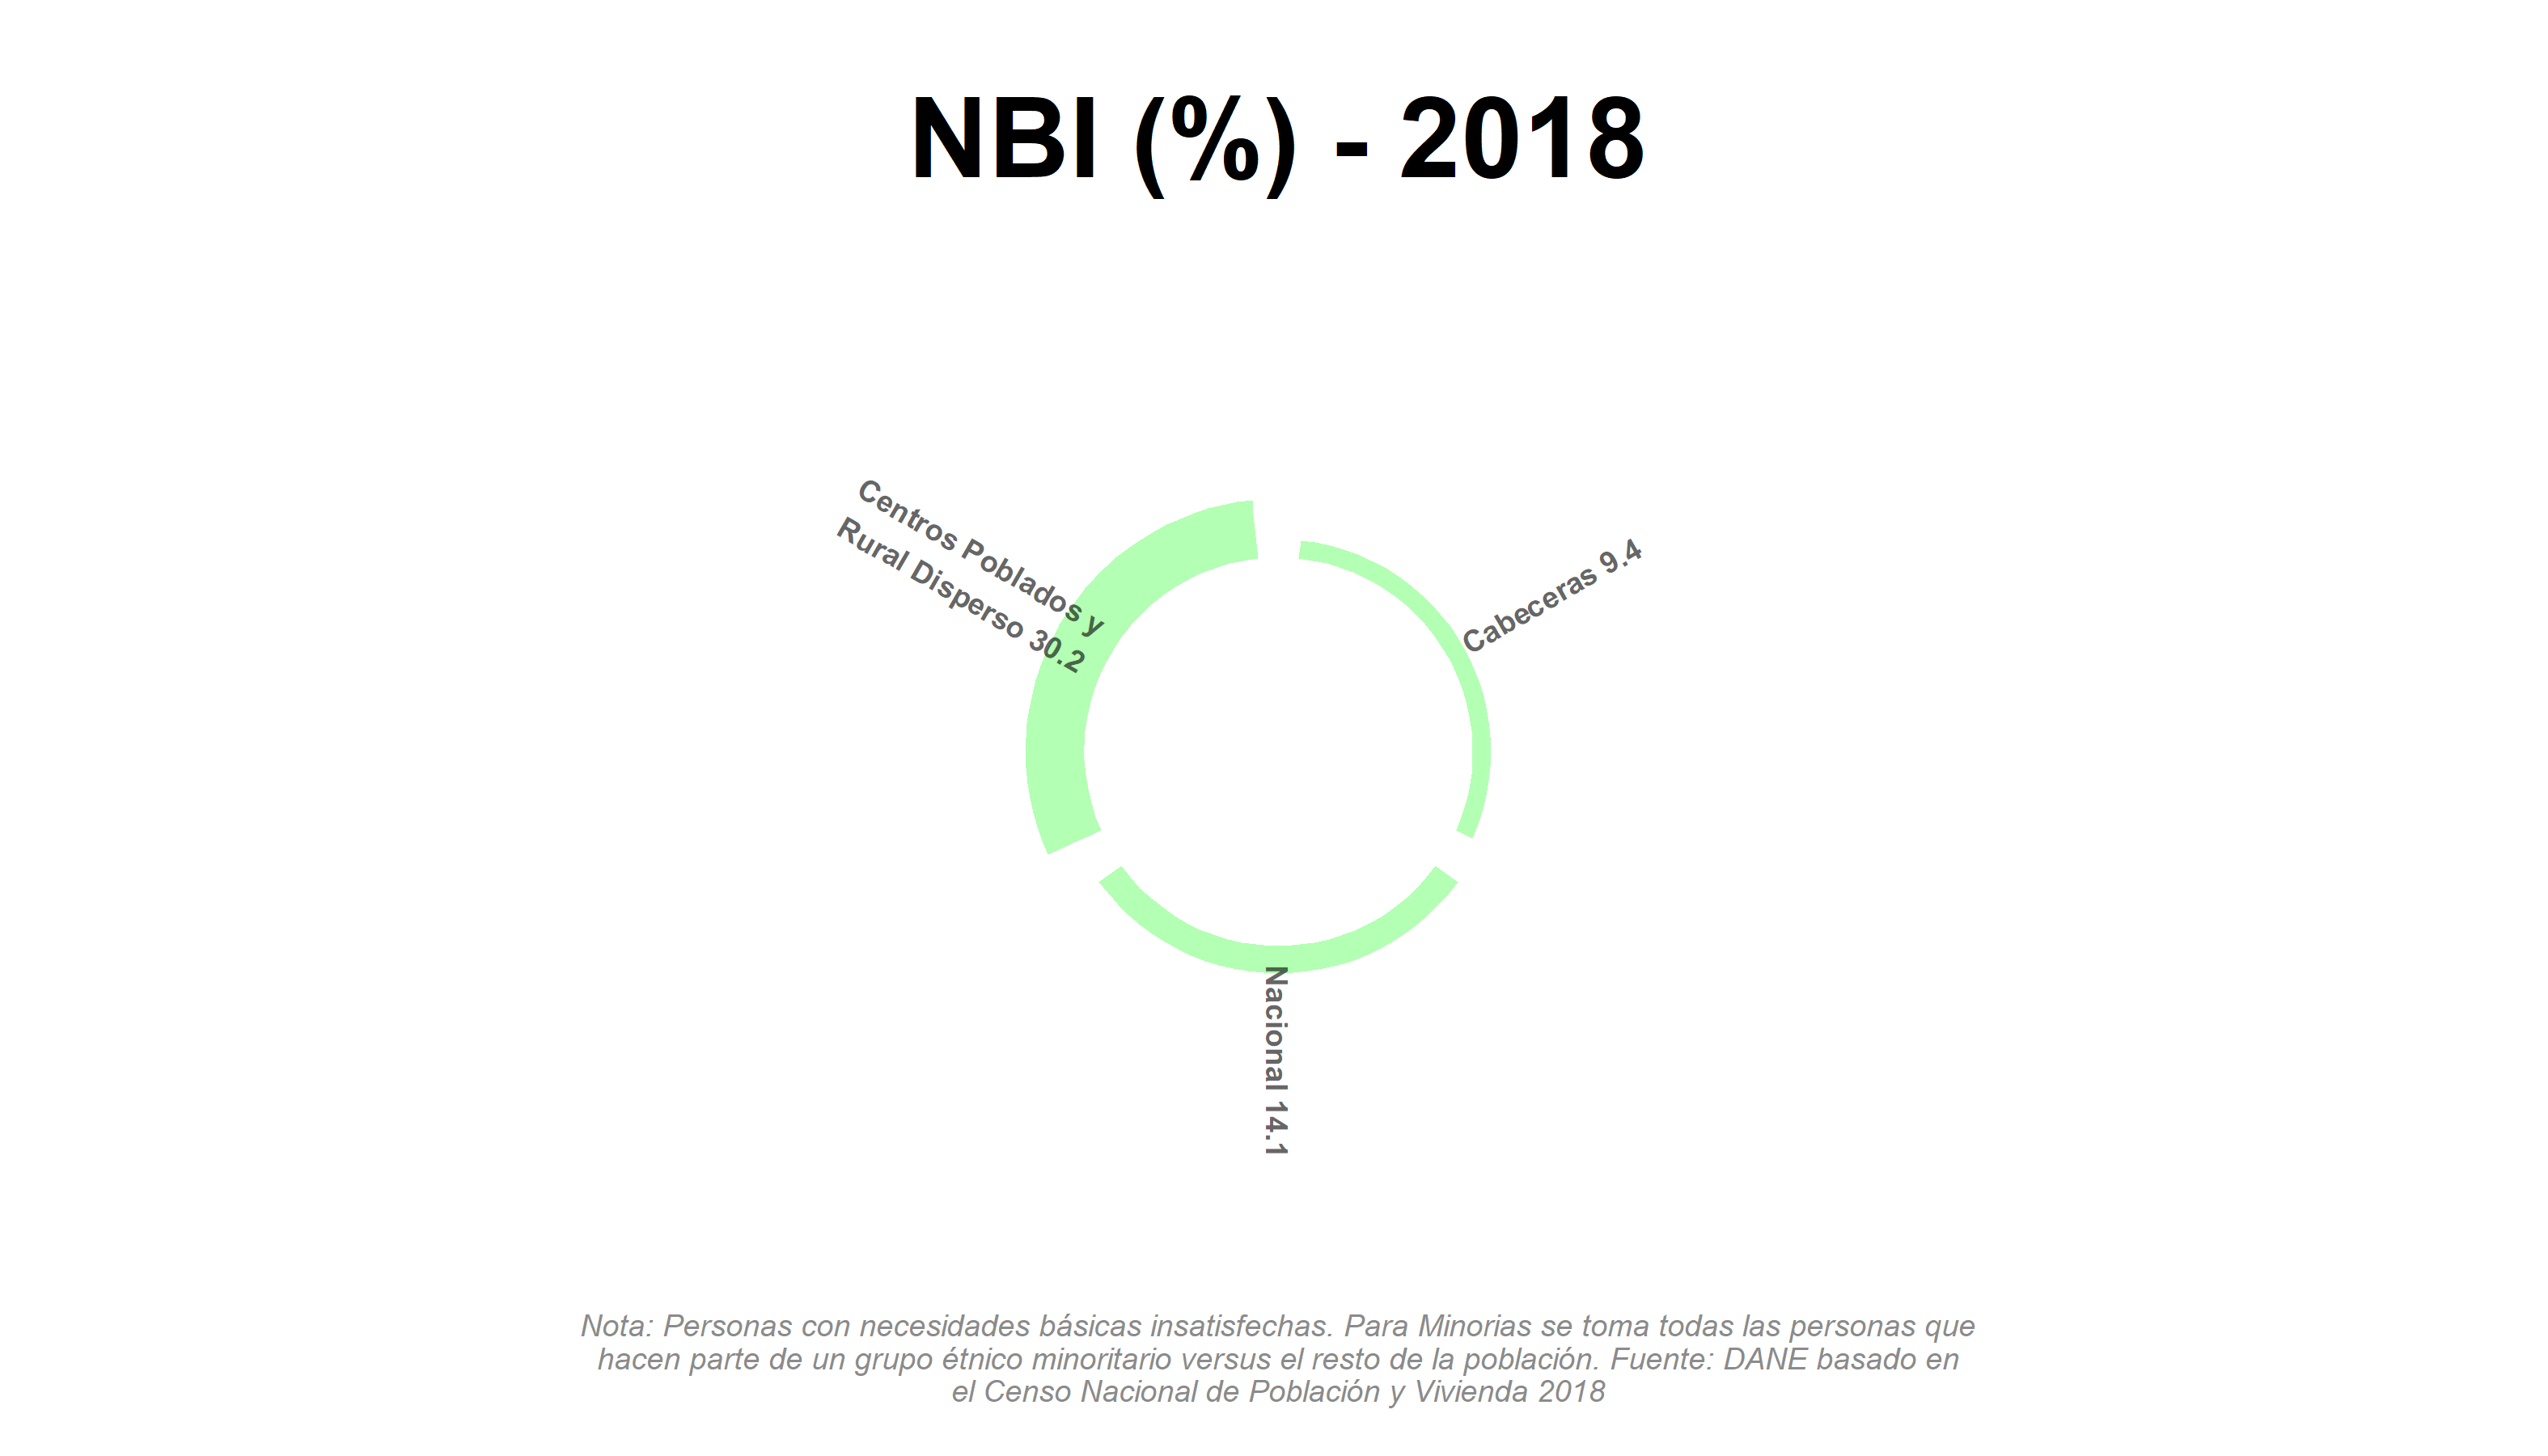
\includegraphics[width=\textwidth,keepaspectratio]{img/var_276_static.png}
        \end{center}
    \end{figure}
            \begin{itemize}
                    \item Los cálculos de las NBI solo están para el 2018 gracias al censo nacional del mismo año, se tiene que a nivel nacional las NBI son del 14.1\%.
                    \item A nivel rural es donde más NBI hay, con un 30.2\%, mientras que las NBI de las cabeceras son del 9.4\%, una diferencia de más del 20\% y siendo las cabeceras menos que el total nacional.n
                    \end{itemize}

\section{Desigualdad}

\begin{figure}[H]
        \caption[Indicador Pulso Social sobre Desigualdad (PCA)]{\label{pca_pobreza} }
        \begin{center}
        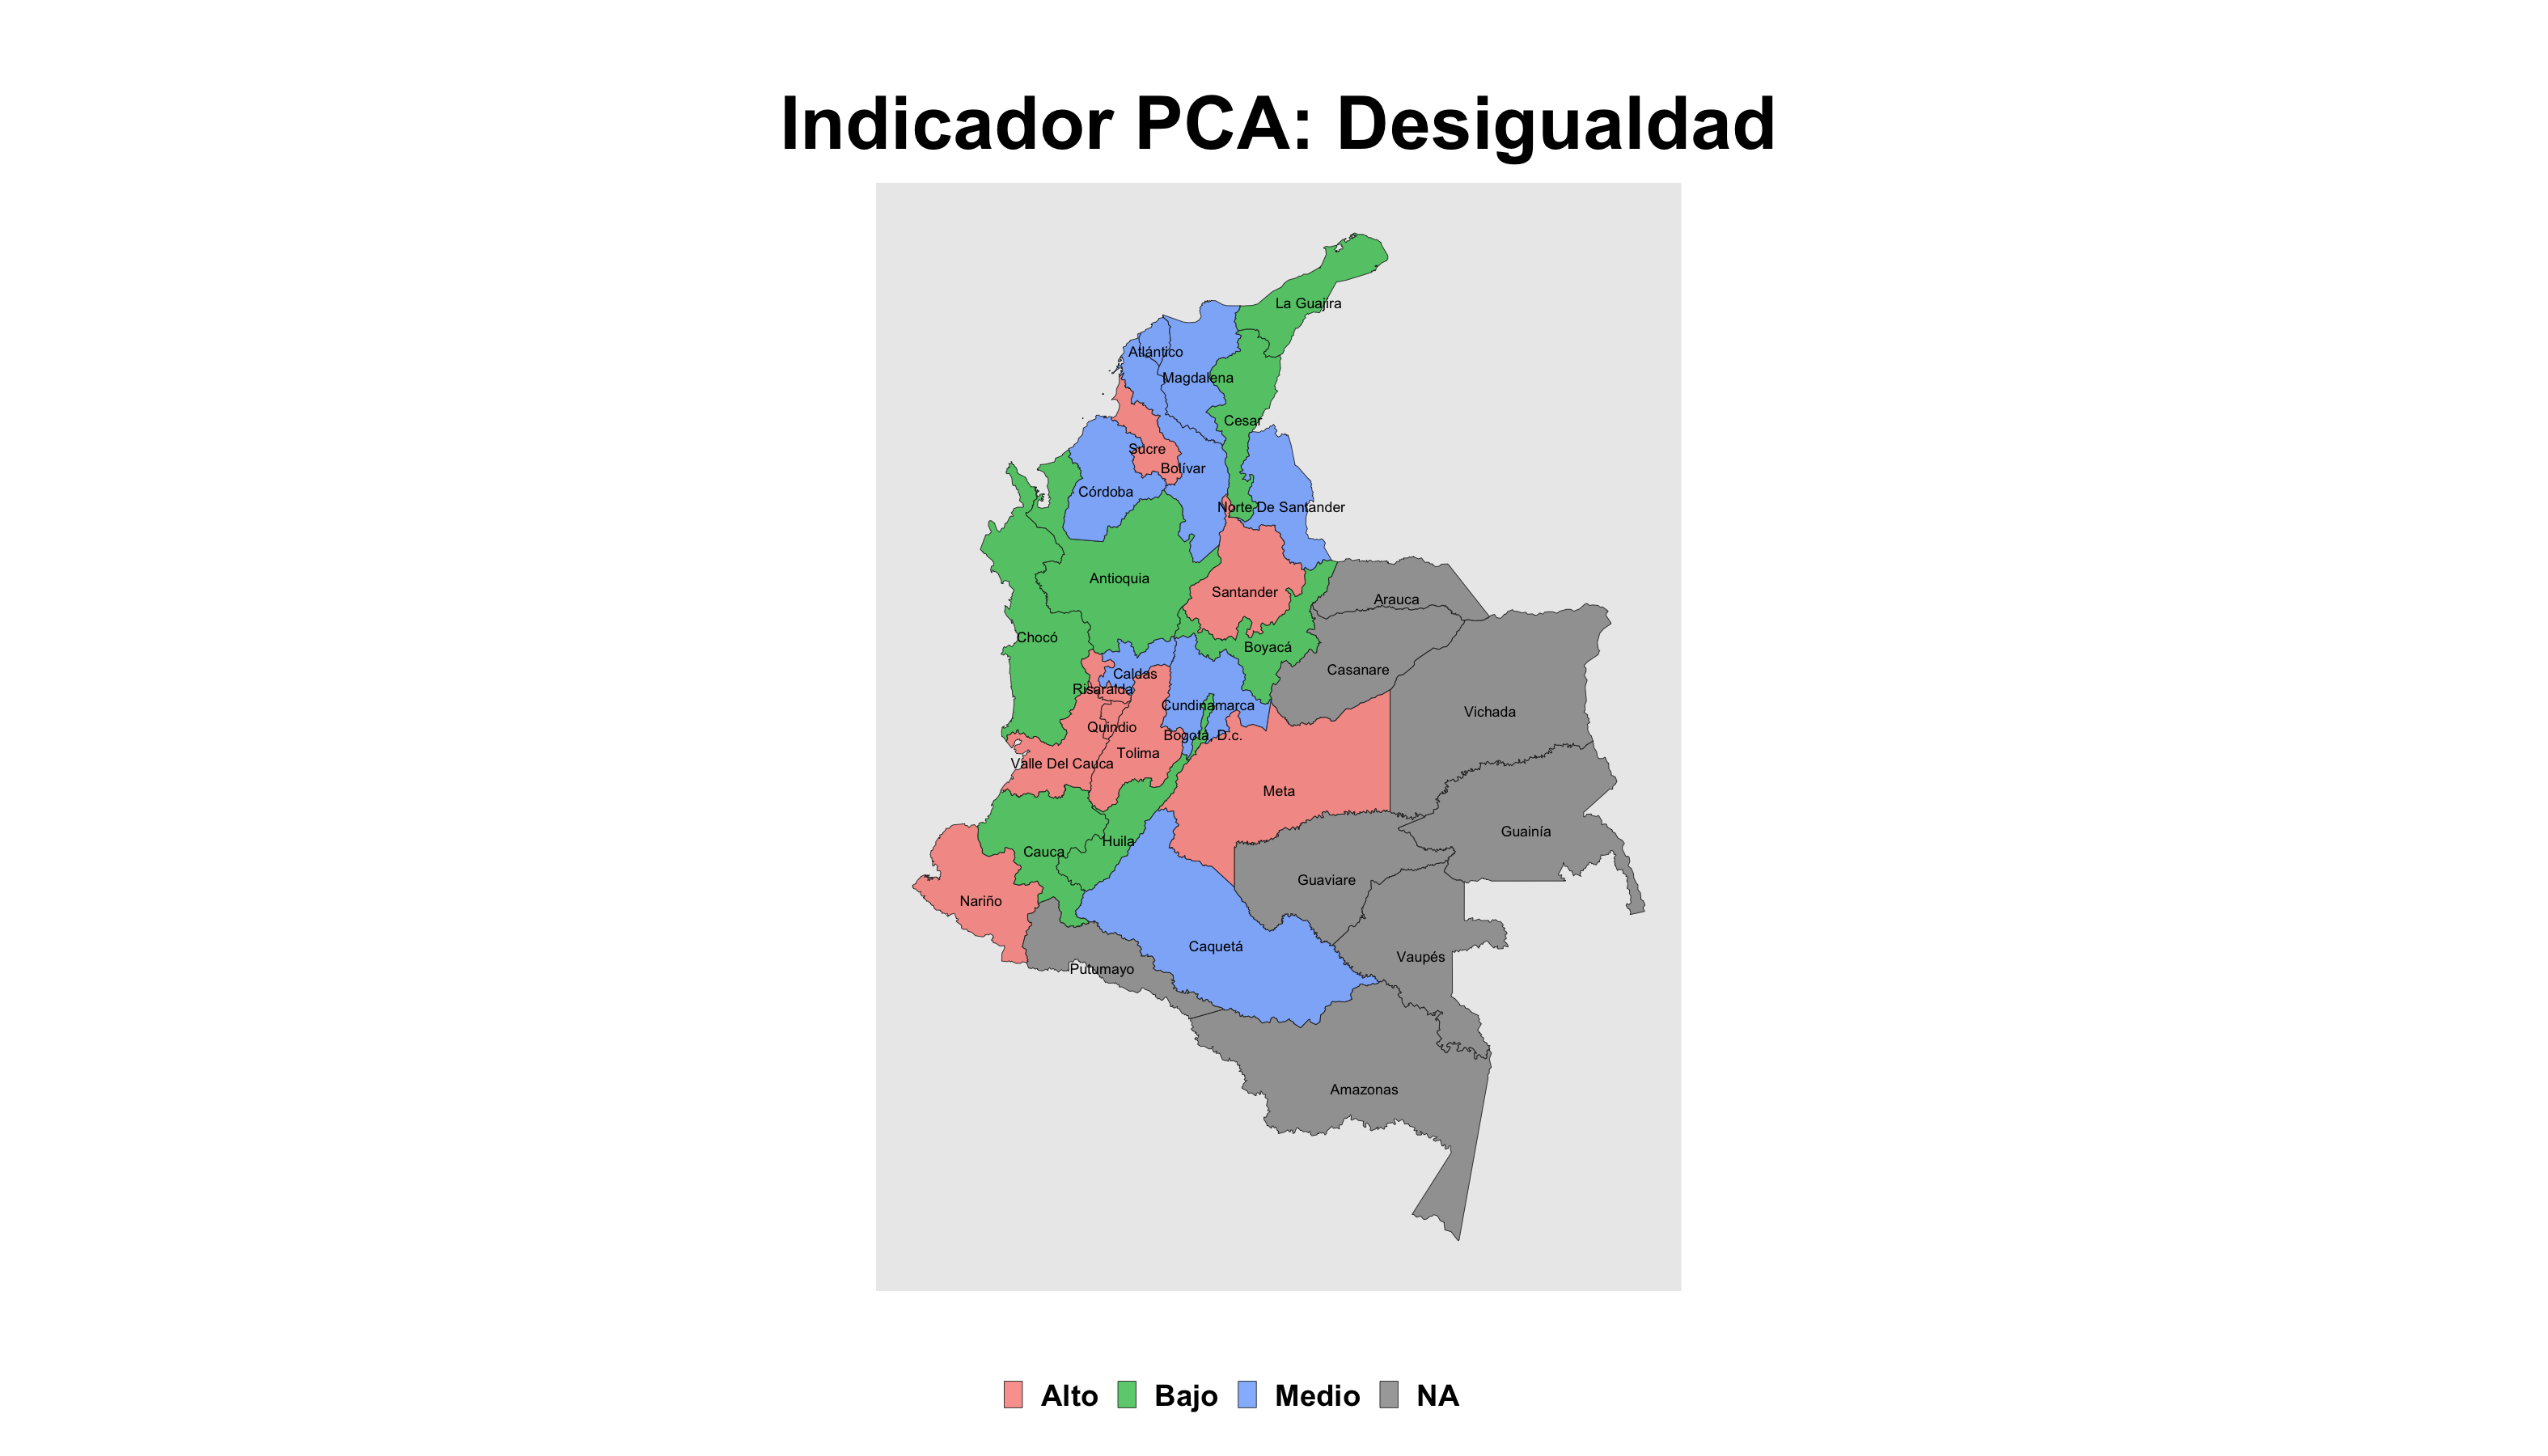
\includegraphics[width=\textwidth,keepaspectratio]{pca_clusters/pca_desigualdad_pca.png}
        \end{center}
    \end{figure}

 %%%%---------------------
    %%% Principales resultados
    %%%%---------------------
    \begin{tcolorbox}[enhanced, colback=mycolor,colframe=mycolor,drop fuzzy shadow,watermark color=white,
                        %%% Título
                        title=Principales Resultados]
    
                    \begin{itemize}
                    \item Pero hay una brecha de género enorme, especialmente en los percentiles más bajos de ingreso.
                    \item El rezago en el ingreso de las mujeres con respecto al de los hombres es de más de 10 años.
                \end{itemize}
     
    \end{tcolorbox}
    %%%%---------------------
    %%%%---------------------
    %%%%---------------------
    
    
    \subsection{Indicadores Convencionales}
        \subsubsection{Coeficiente de Gini}

%%%% Include figures
    \begin{figure}[H]
        \caption[Coeficiente de Gini por ciudades - 2002 VS 2020 ]{\label{gini_ciudades_vs} }
        \begin{center}
        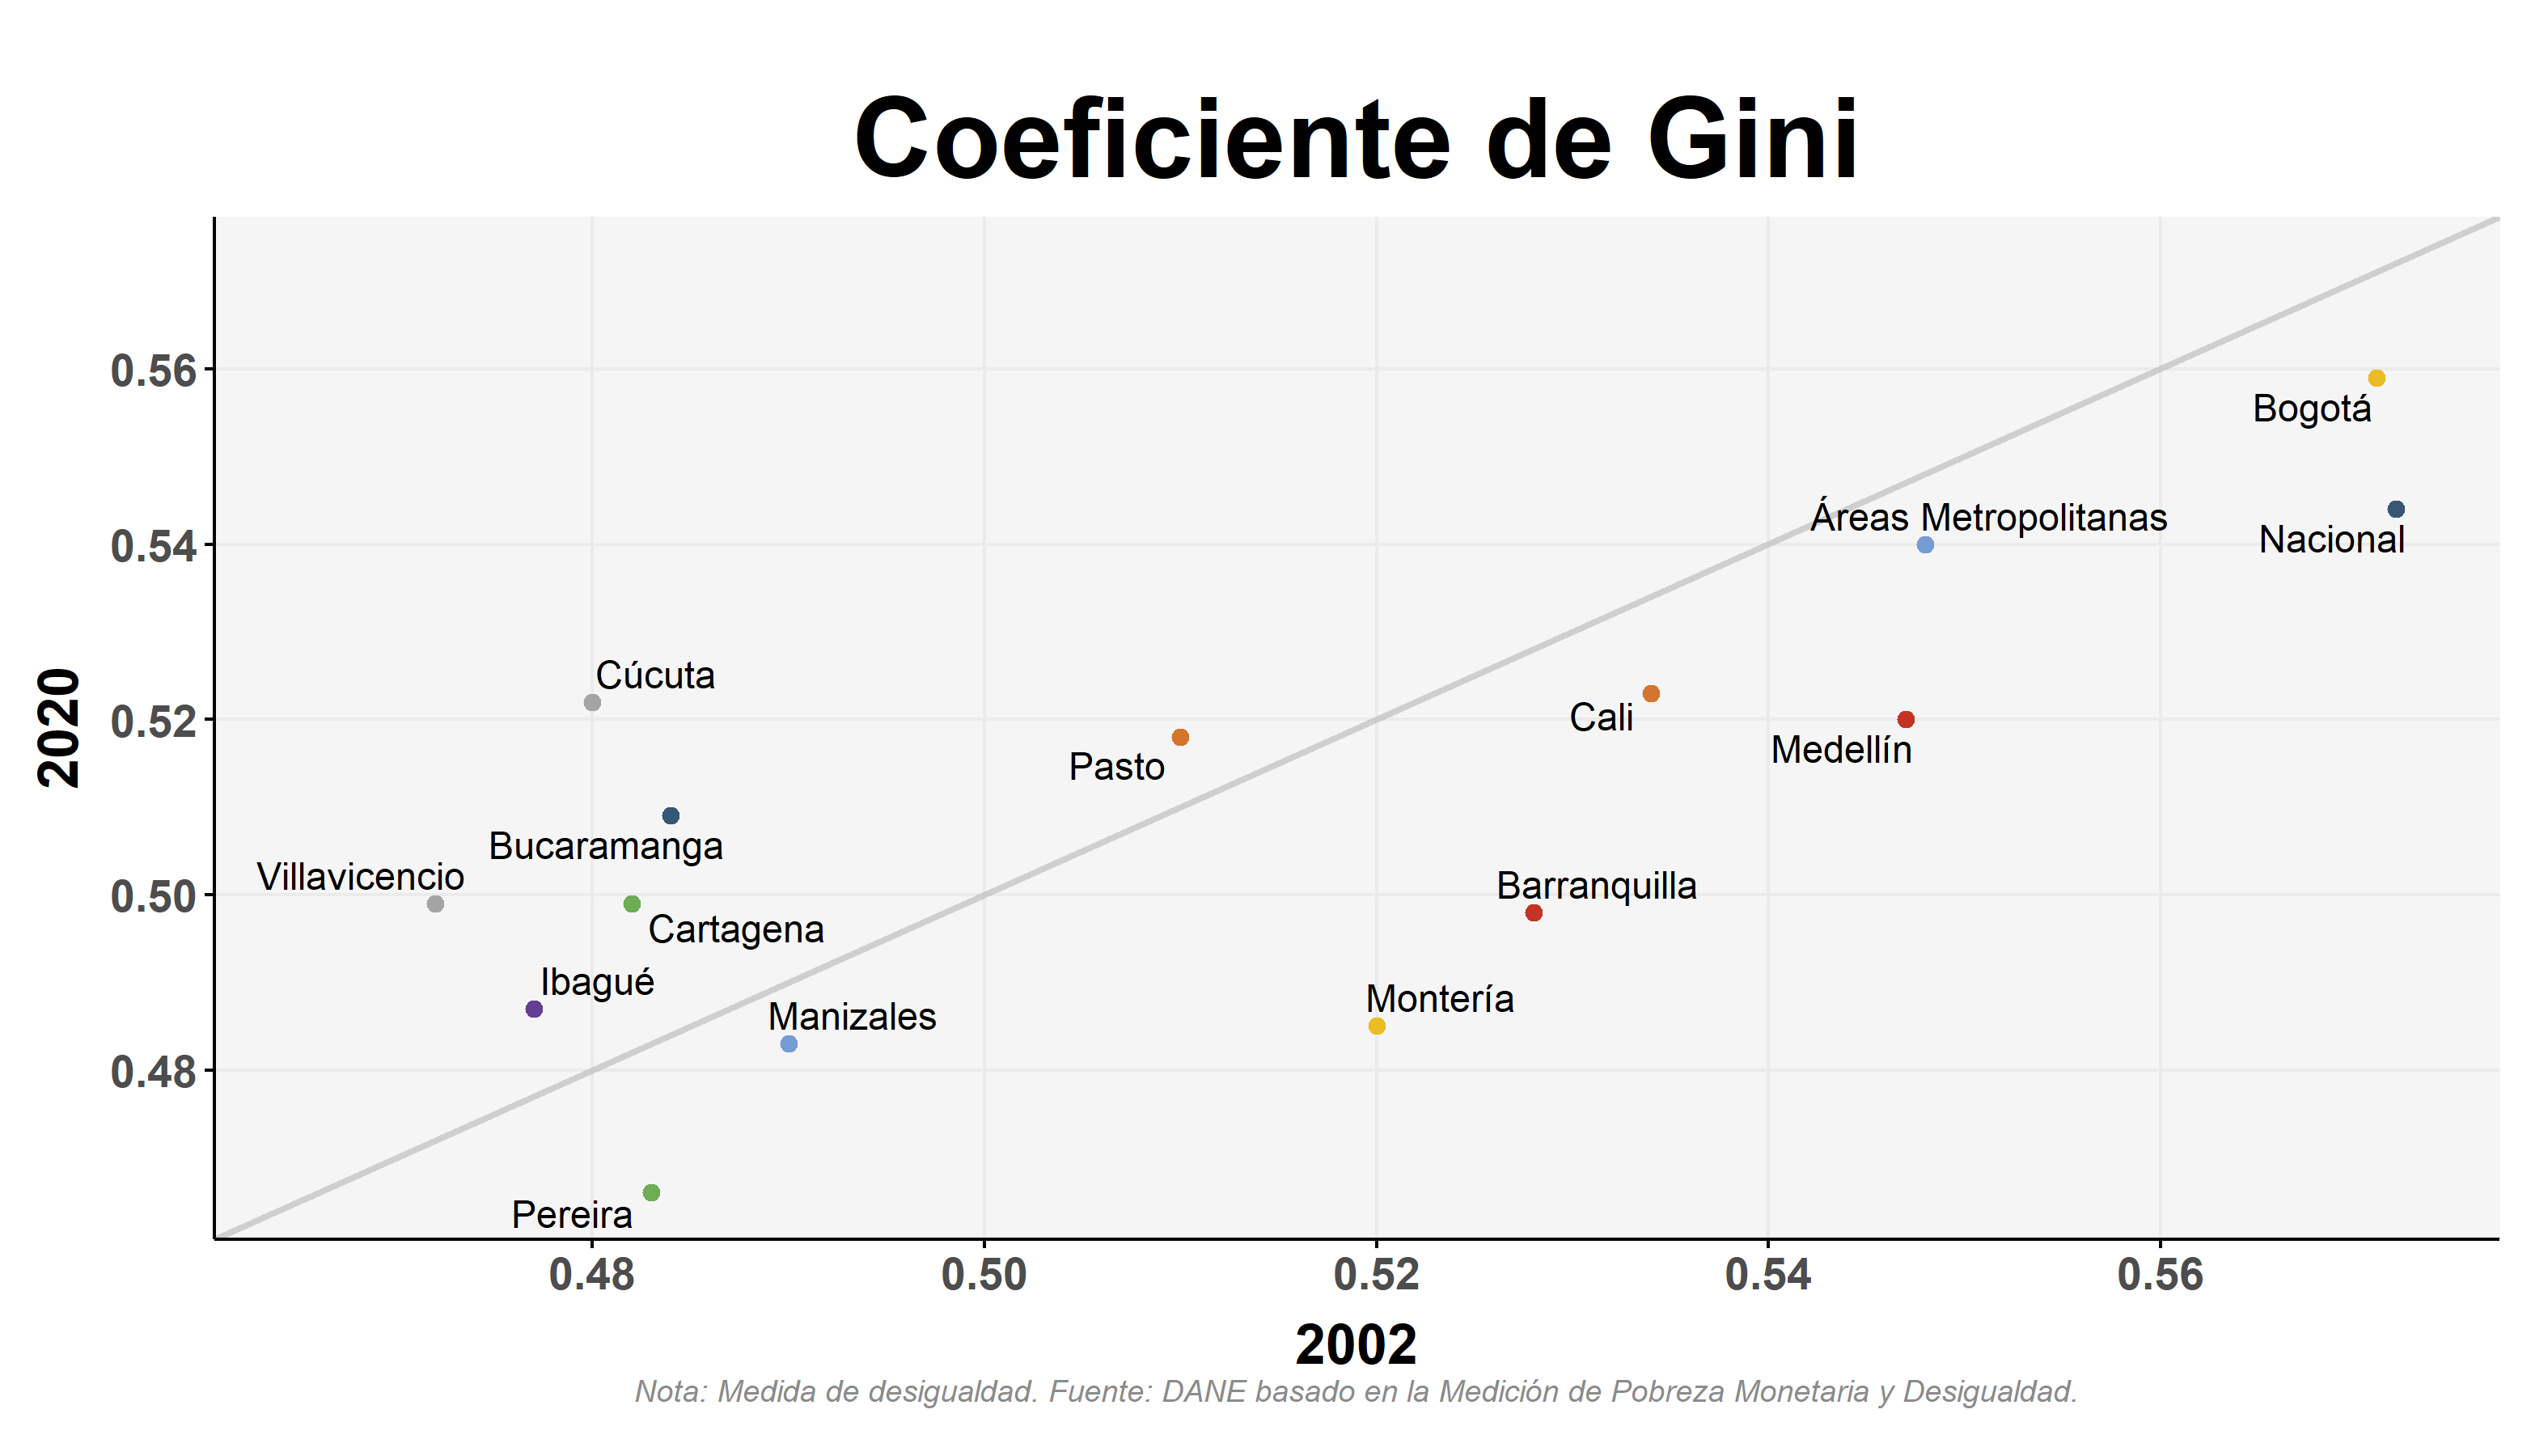
\includegraphics[width=\textwidth,keepaspectratio]{img/var_253_scatter_time.png}
        \end{center}
    \end{figure}
            \begin{itemize}
                    \item En general la mayoría de las ciudades mejoraron sus niveles de desigualdad.
                    \item Cúcuta, Bucaramanga y Villavicencio son las ciudades que aumentaron los niveles de desigualdad que tenían hace casi 20 años.
                    \item Manizáles, Bogotá y Pasto se podría decir que se mantuvieron cerca de los niveles de desigualdad que tenían en 2002.
                    \item Bogotá sigue siendo la ciudad con mayor nivel de desigualdad, mientras que la de menor es Pereira.
                    \end{itemize}

%%%% Include figures
    \begin{figure}[H]
        \caption[Coeficiente de Gini por departamentos - 2002 VS 2020 ]{\label{gini_dptos_vs} }
        \begin{center}
        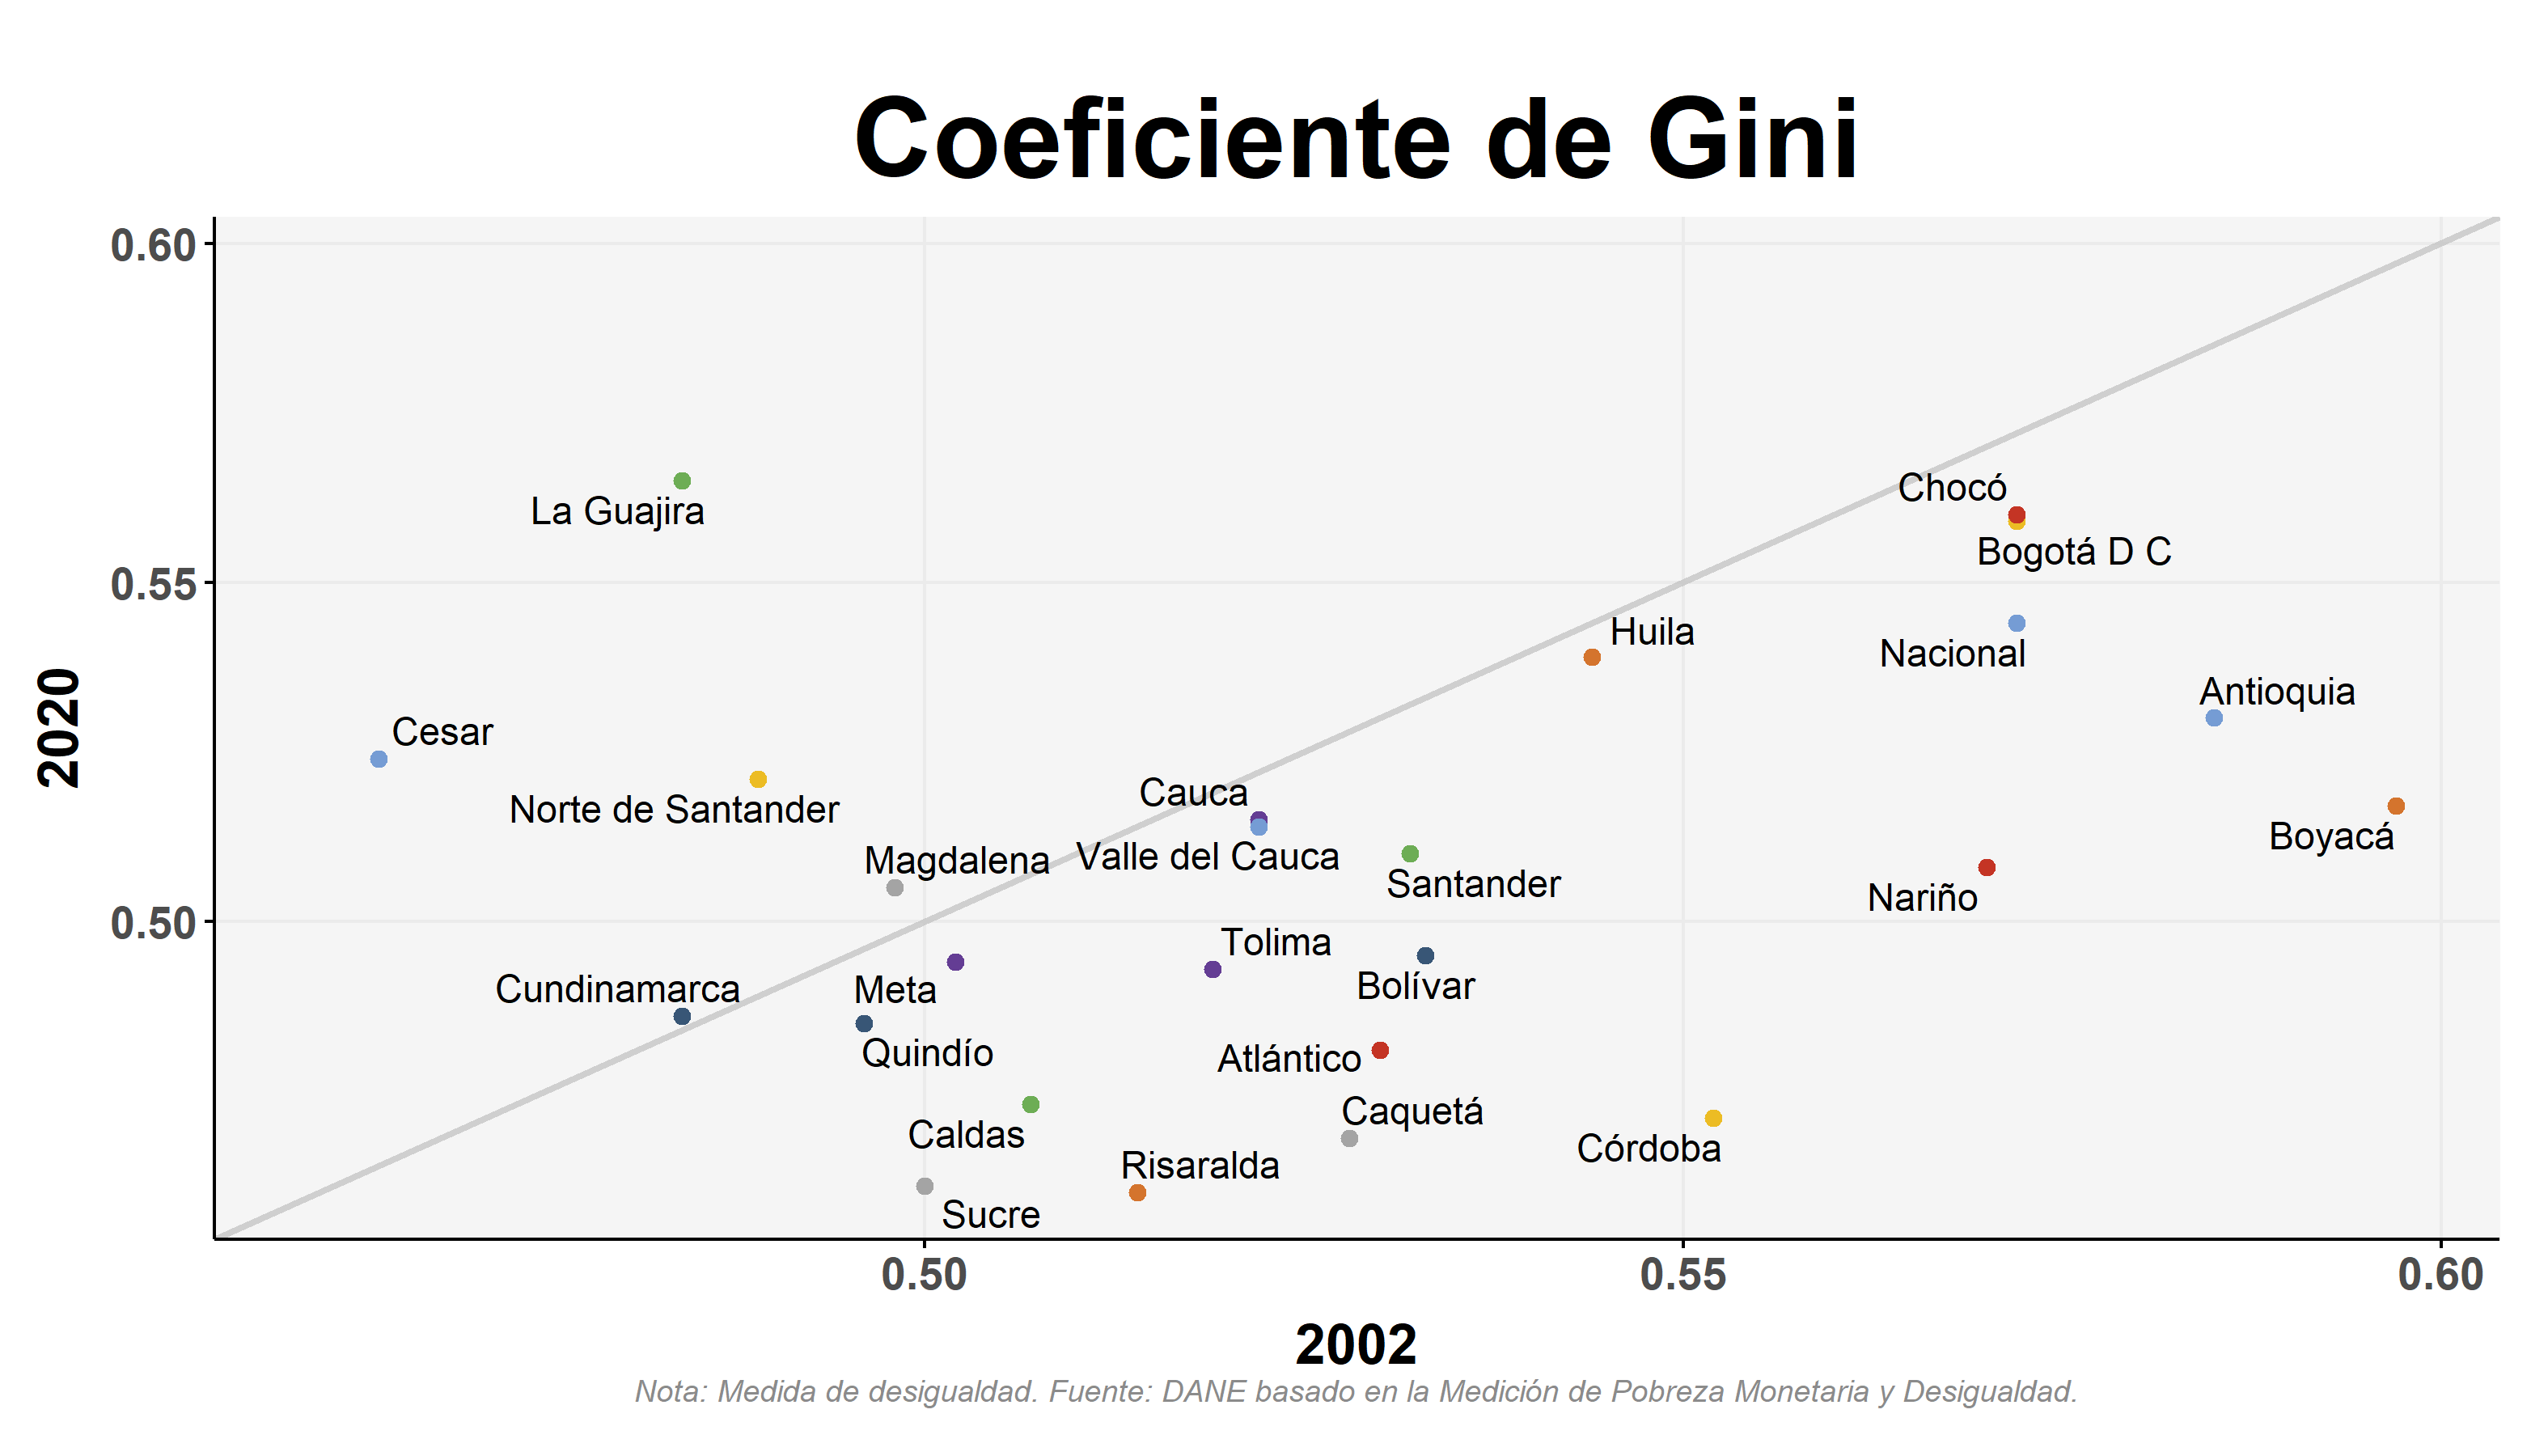
\includegraphics[width=\textwidth,keepaspectratio]{img/var_254_scatter_time.png}
        \end{center}
    \end{figure}
            \begin{itemize}
                    \item Gran parte de los territorios mostró una mejorías en la desigualdad.
                    \item Departamentos como Huila, Cauca y Cundinamarca están cerca de los niveles reportados 18 años atrás.
                    \item La Guajira a pesar de en el 2002 ser de los departamentos con menor desigualdad, para el 2020 es el de mayor según el coeficiente de Gini.
                    \item Risaralda es el dpto con menor desigualdad, aunque cabe mencionar que la distribución no es tan amplia (0.45 a 0.55).
                    \end{itemize}

%%%% Include figures
    \begin{figure}[H]
        \caption[Coeficiente de Gini por zonas y nacional ]{\label{gini_zonas} }
        \begin{center}
        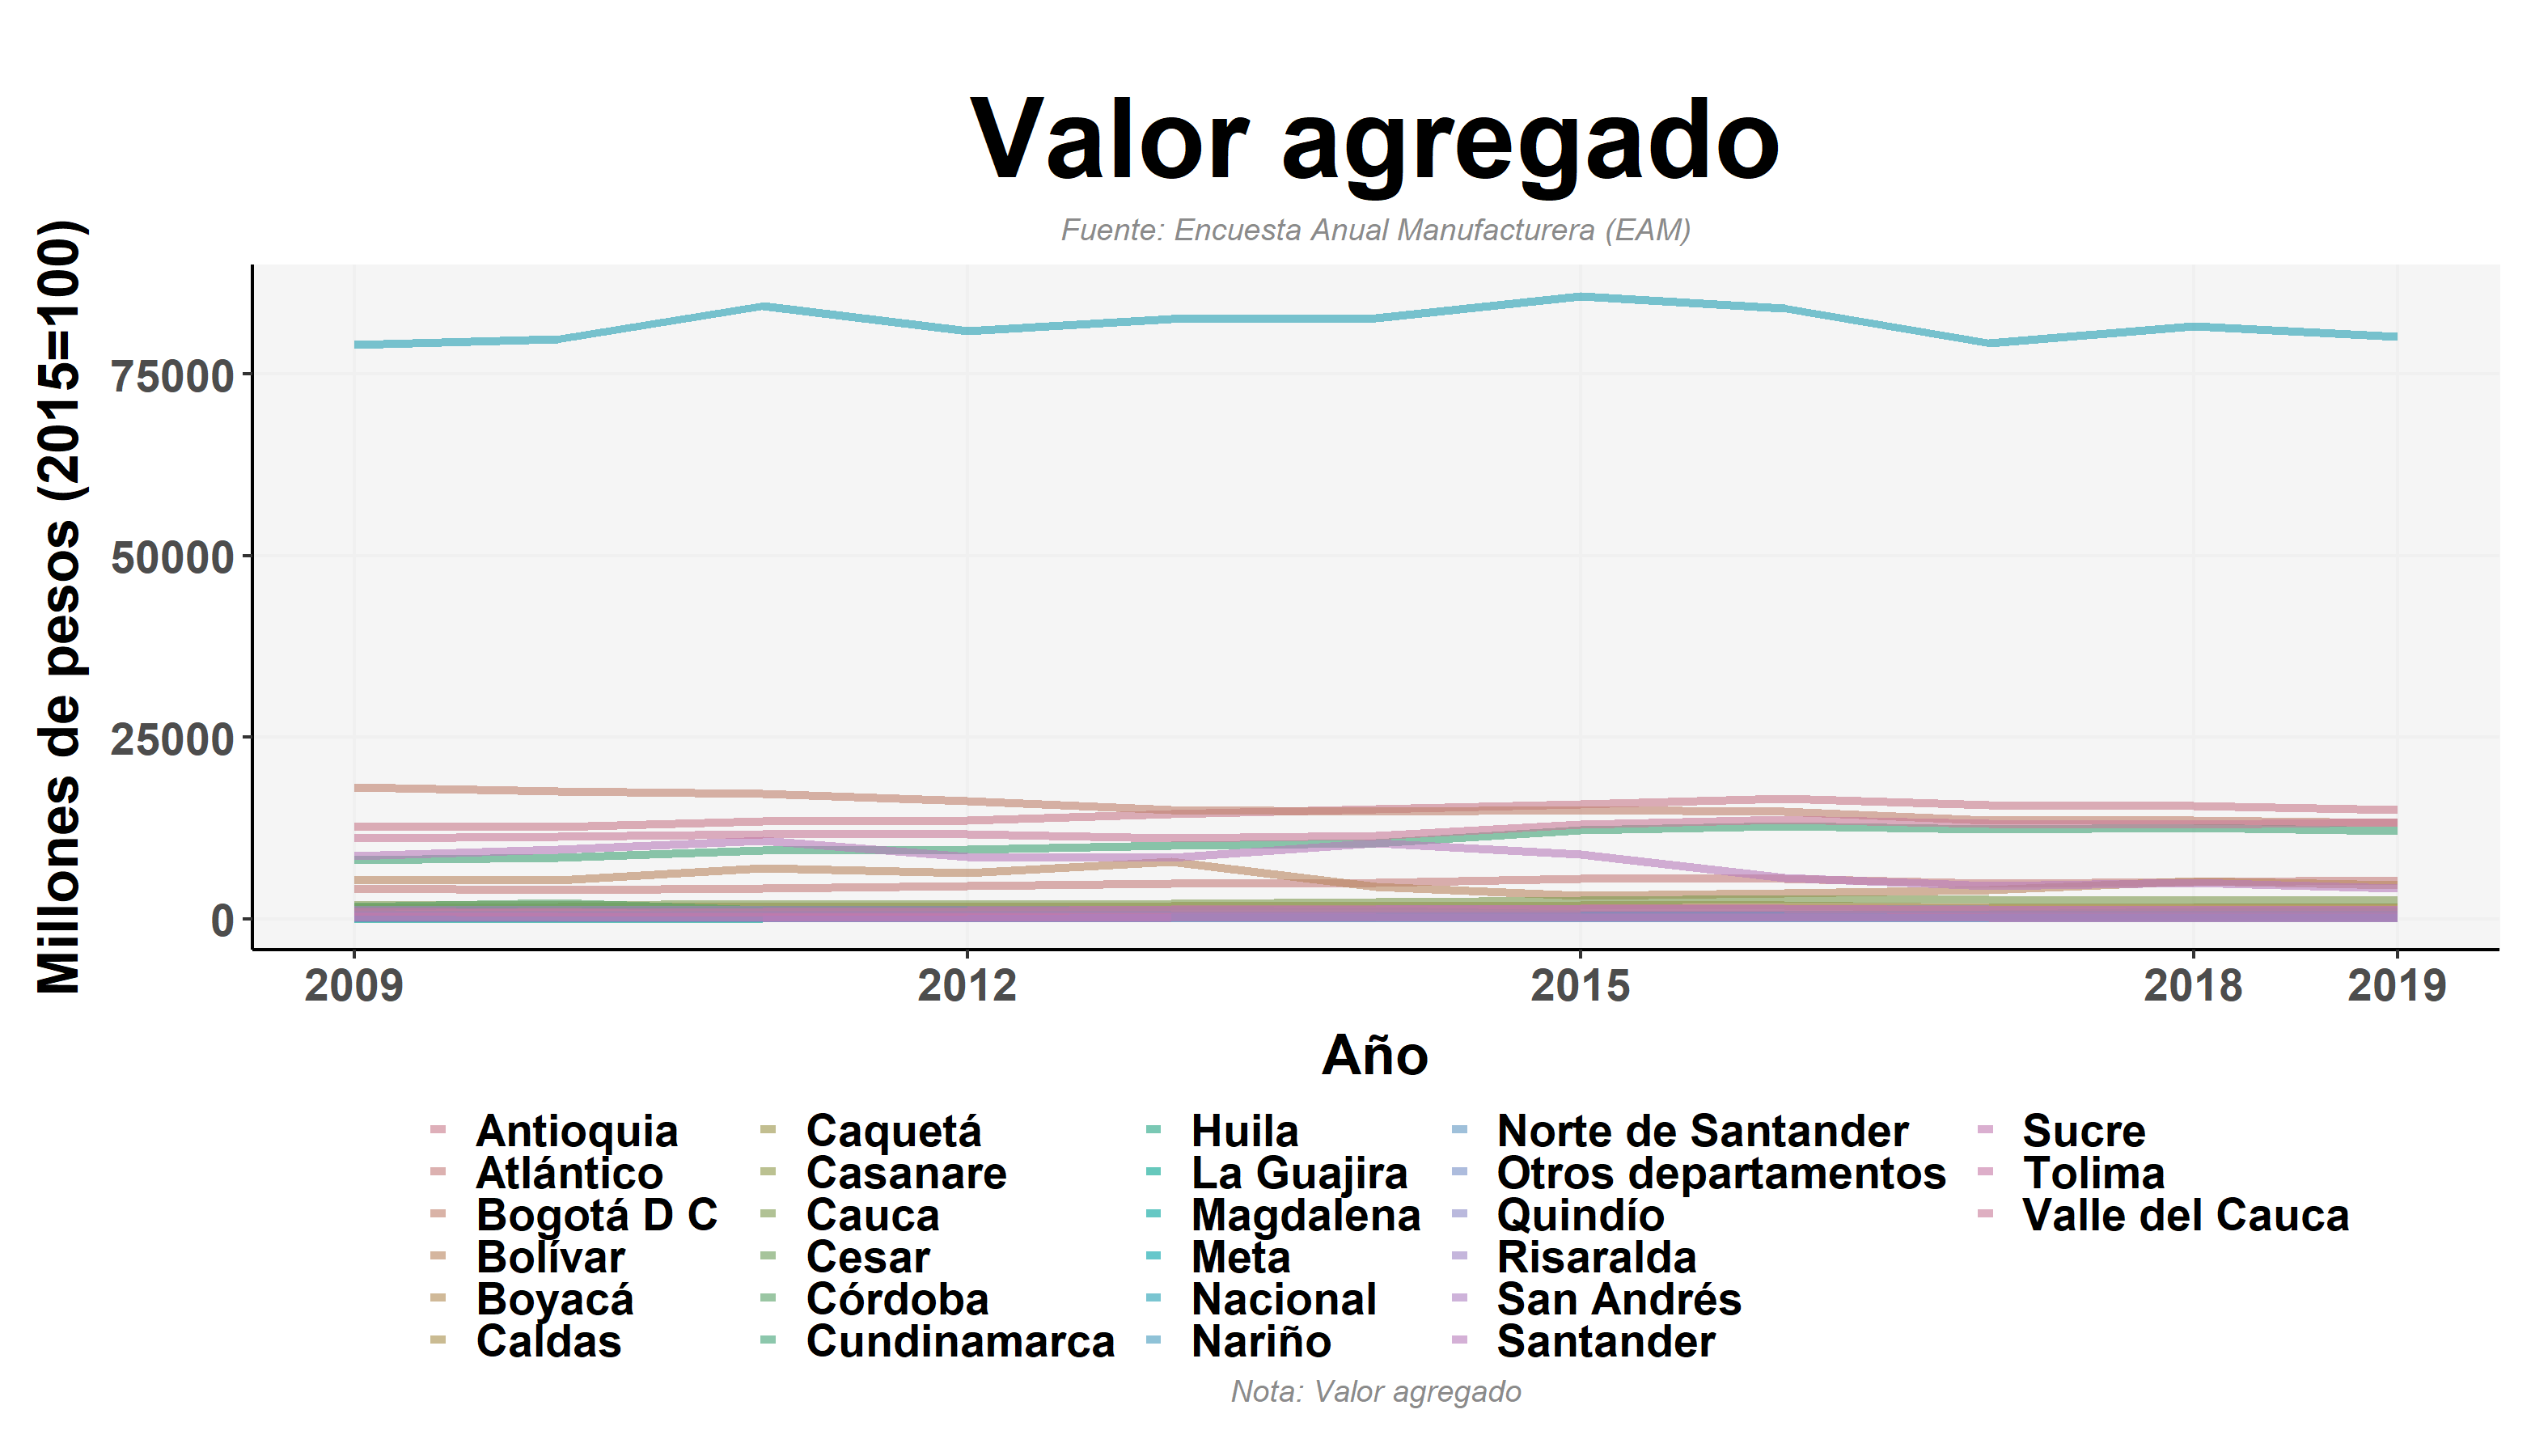
\includegraphics[width=\textwidth,keepaspectratio]{img/var_256_trend.png}
        \end{center}
    \end{figure}
            \begin{itemize}
                    \item A nivel de zonas se encontró que desde el 2008 se veía una tendencia a la baja hasta el 2017 donde volvió a aumentar, a excepción de la zona rural, que se intensificó en el 2020.
                    \item La zona rural ha mostrado tener los niveles de desigualdad más bajo, manteniendo niveles similares desde el 2014.
                    \item Para el 2020 las cabeceras y a nivel nacional tuvieron una menor brecha, alcanzando niveles similares.
                    \item Para las otras cabeceras el comportamiento es igual que el de las cabeceras, pero con menor intensidad en el caso del 2020.
                    \end{itemize}

\section{Características de las Viviendas}

\begin{figure}[H]
        \caption[Indicador Pulso Social sobre Características de la Vivienda (PCA)]{\label{pca_pobreza} }
        \begin{center}
        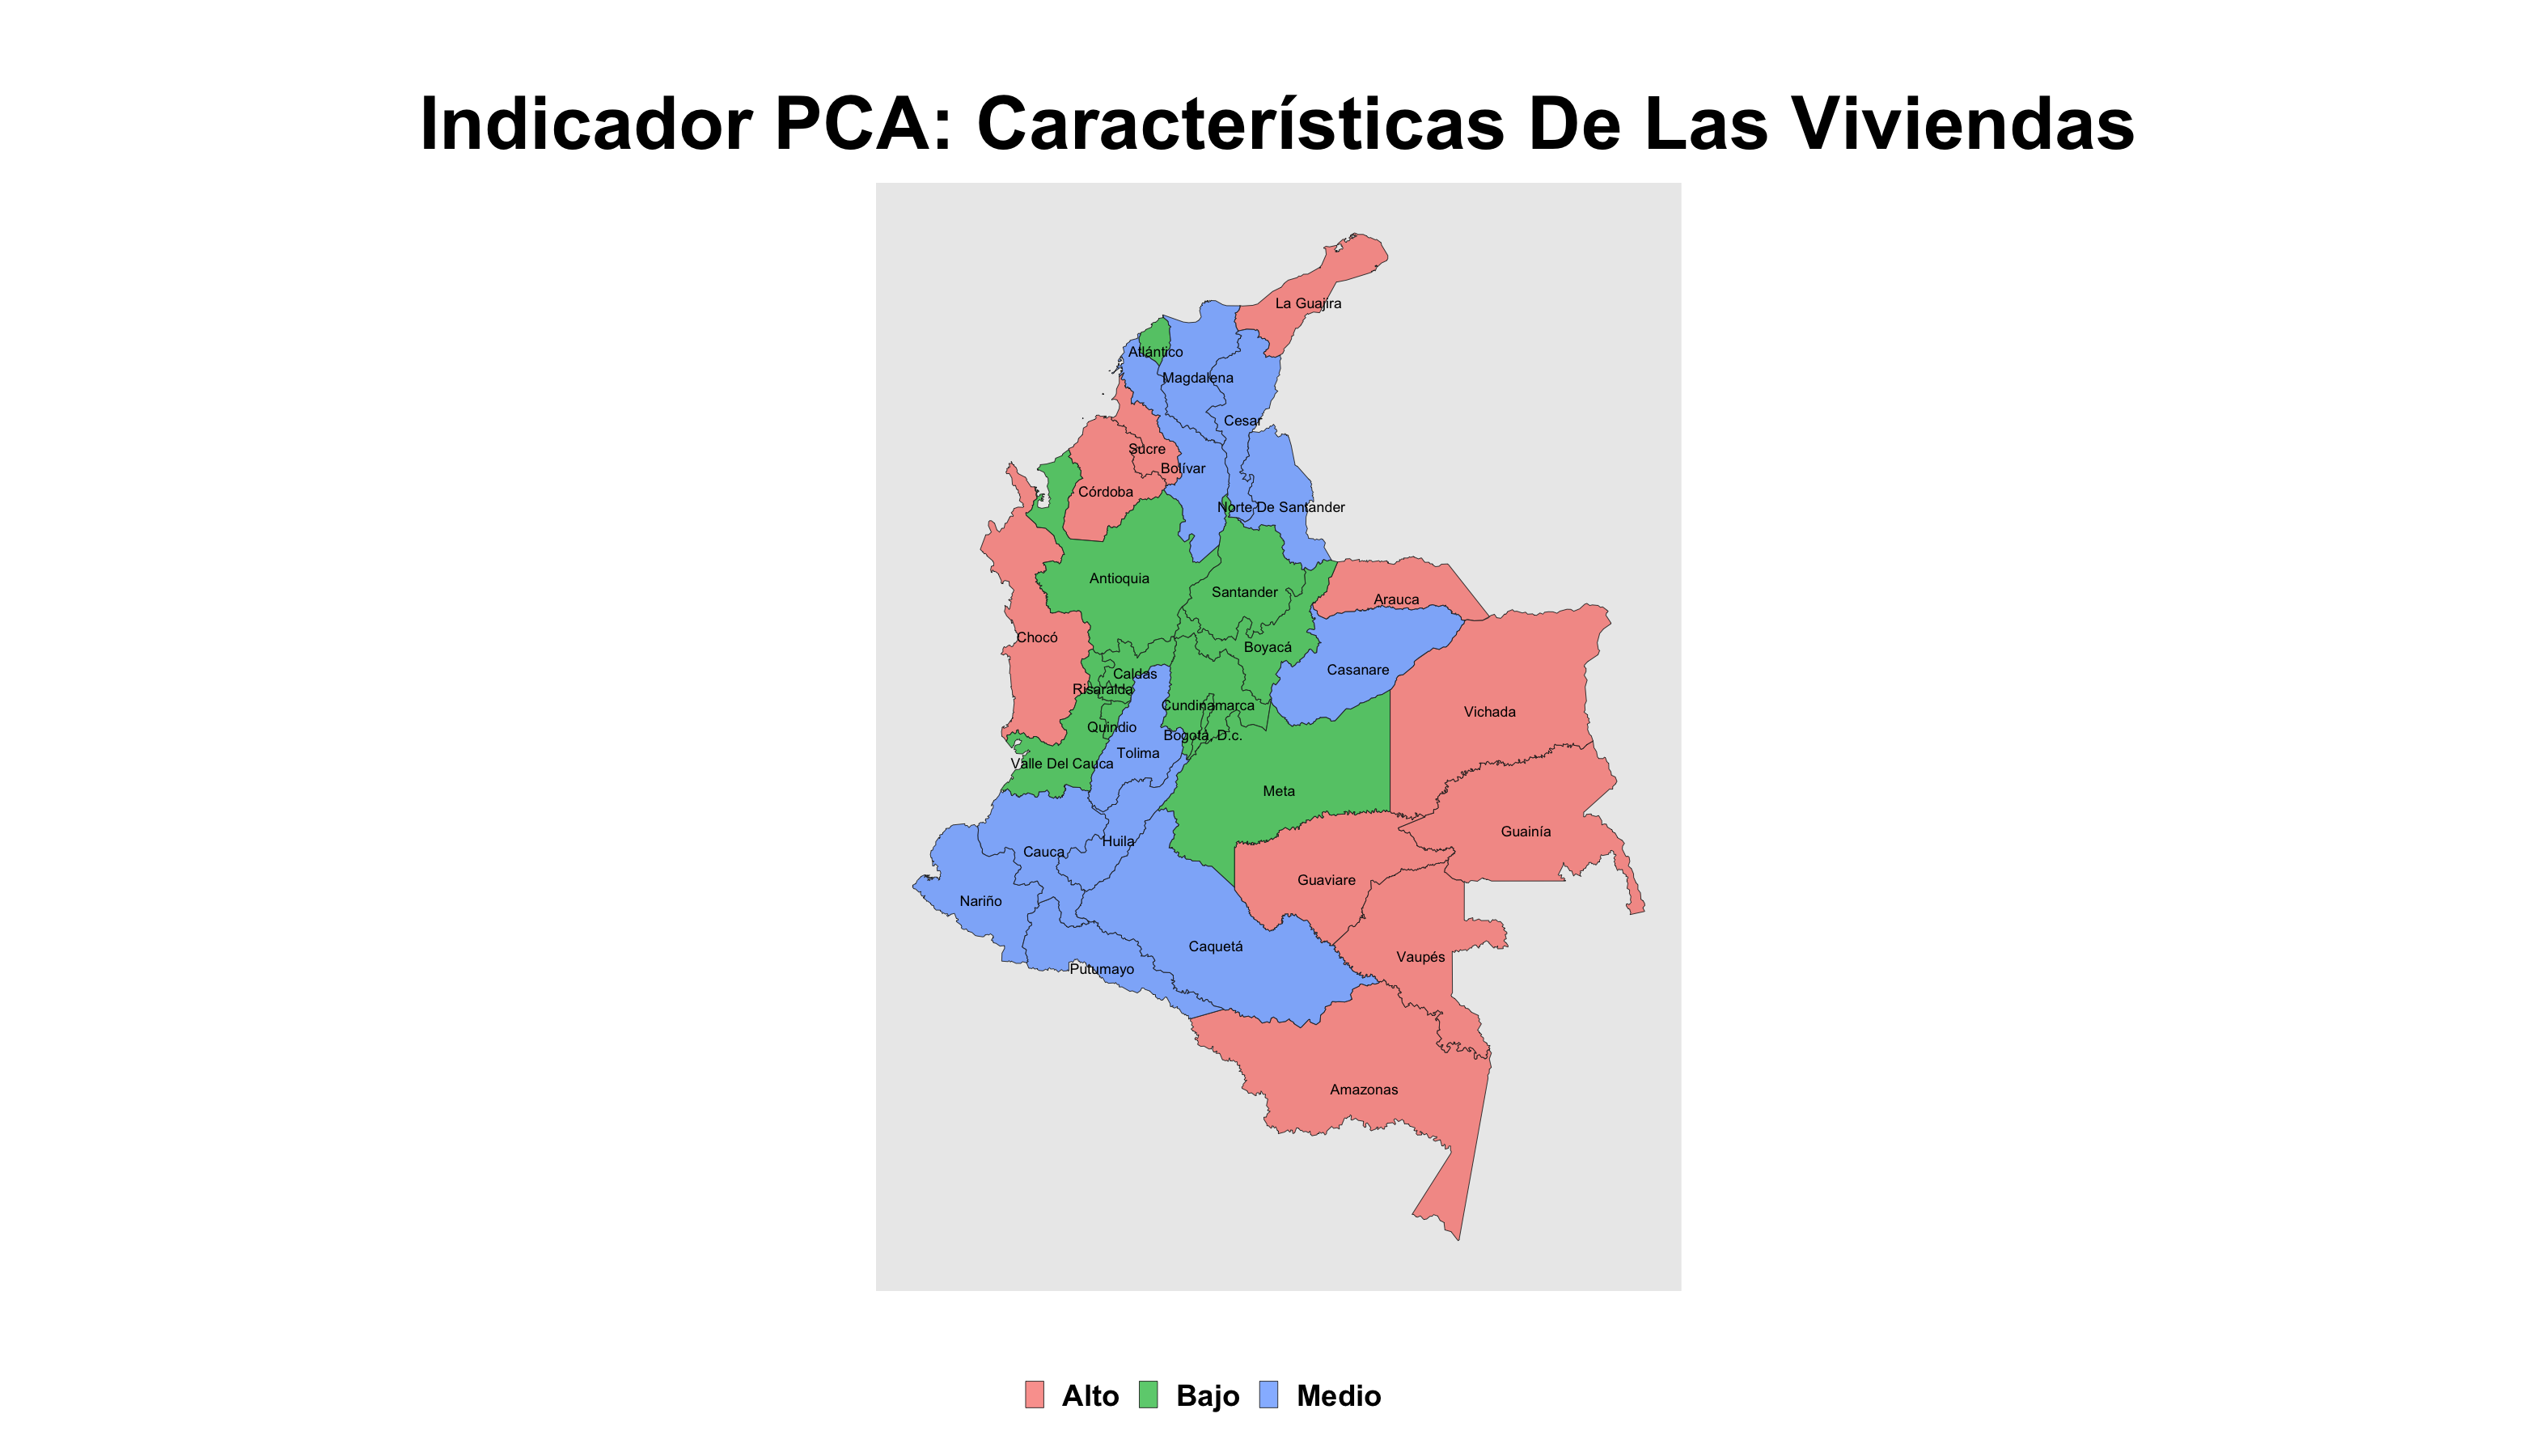
\includegraphics[width=\textwidth,keepaspectratio]{pca_clusters/pca_caracteristicas_de_las_viviendas_pca.png}
        \end{center}
    \end{figure}

 %%%%---------------------
    %%% Principales resultados
    %%%%---------------------
    \begin{tcolorbox}[enhanced, colback=mycolor,colframe=mycolor,drop fuzzy shadow,watermark color=white,
                        %%% Título
                        title=Principales Resultados]
    
                    \begin{itemize}
                    \item Pero hay una brecha de género enorme, especialmente en los percentiles más bajos de ingreso.
                    \item El rezago en el ingreso de las mujeres con respecto al de los hombres es de más de 10 años.
                \end{itemize}
     
    \end{tcolorbox}
    %%%%---------------------
    %%%%---------------------
    %%%%---------------------
    
    
    \subsection{Calidad de los Materiales}
        \subsubsection{Material de la Pared}

%%%% Include figures
    \begin{figure}[H]
        \caption[Viviendas con pared de ladrillo por departamentos para 2020 ]{\label{pared_ladrillo_dptos} }
        \begin{center}
        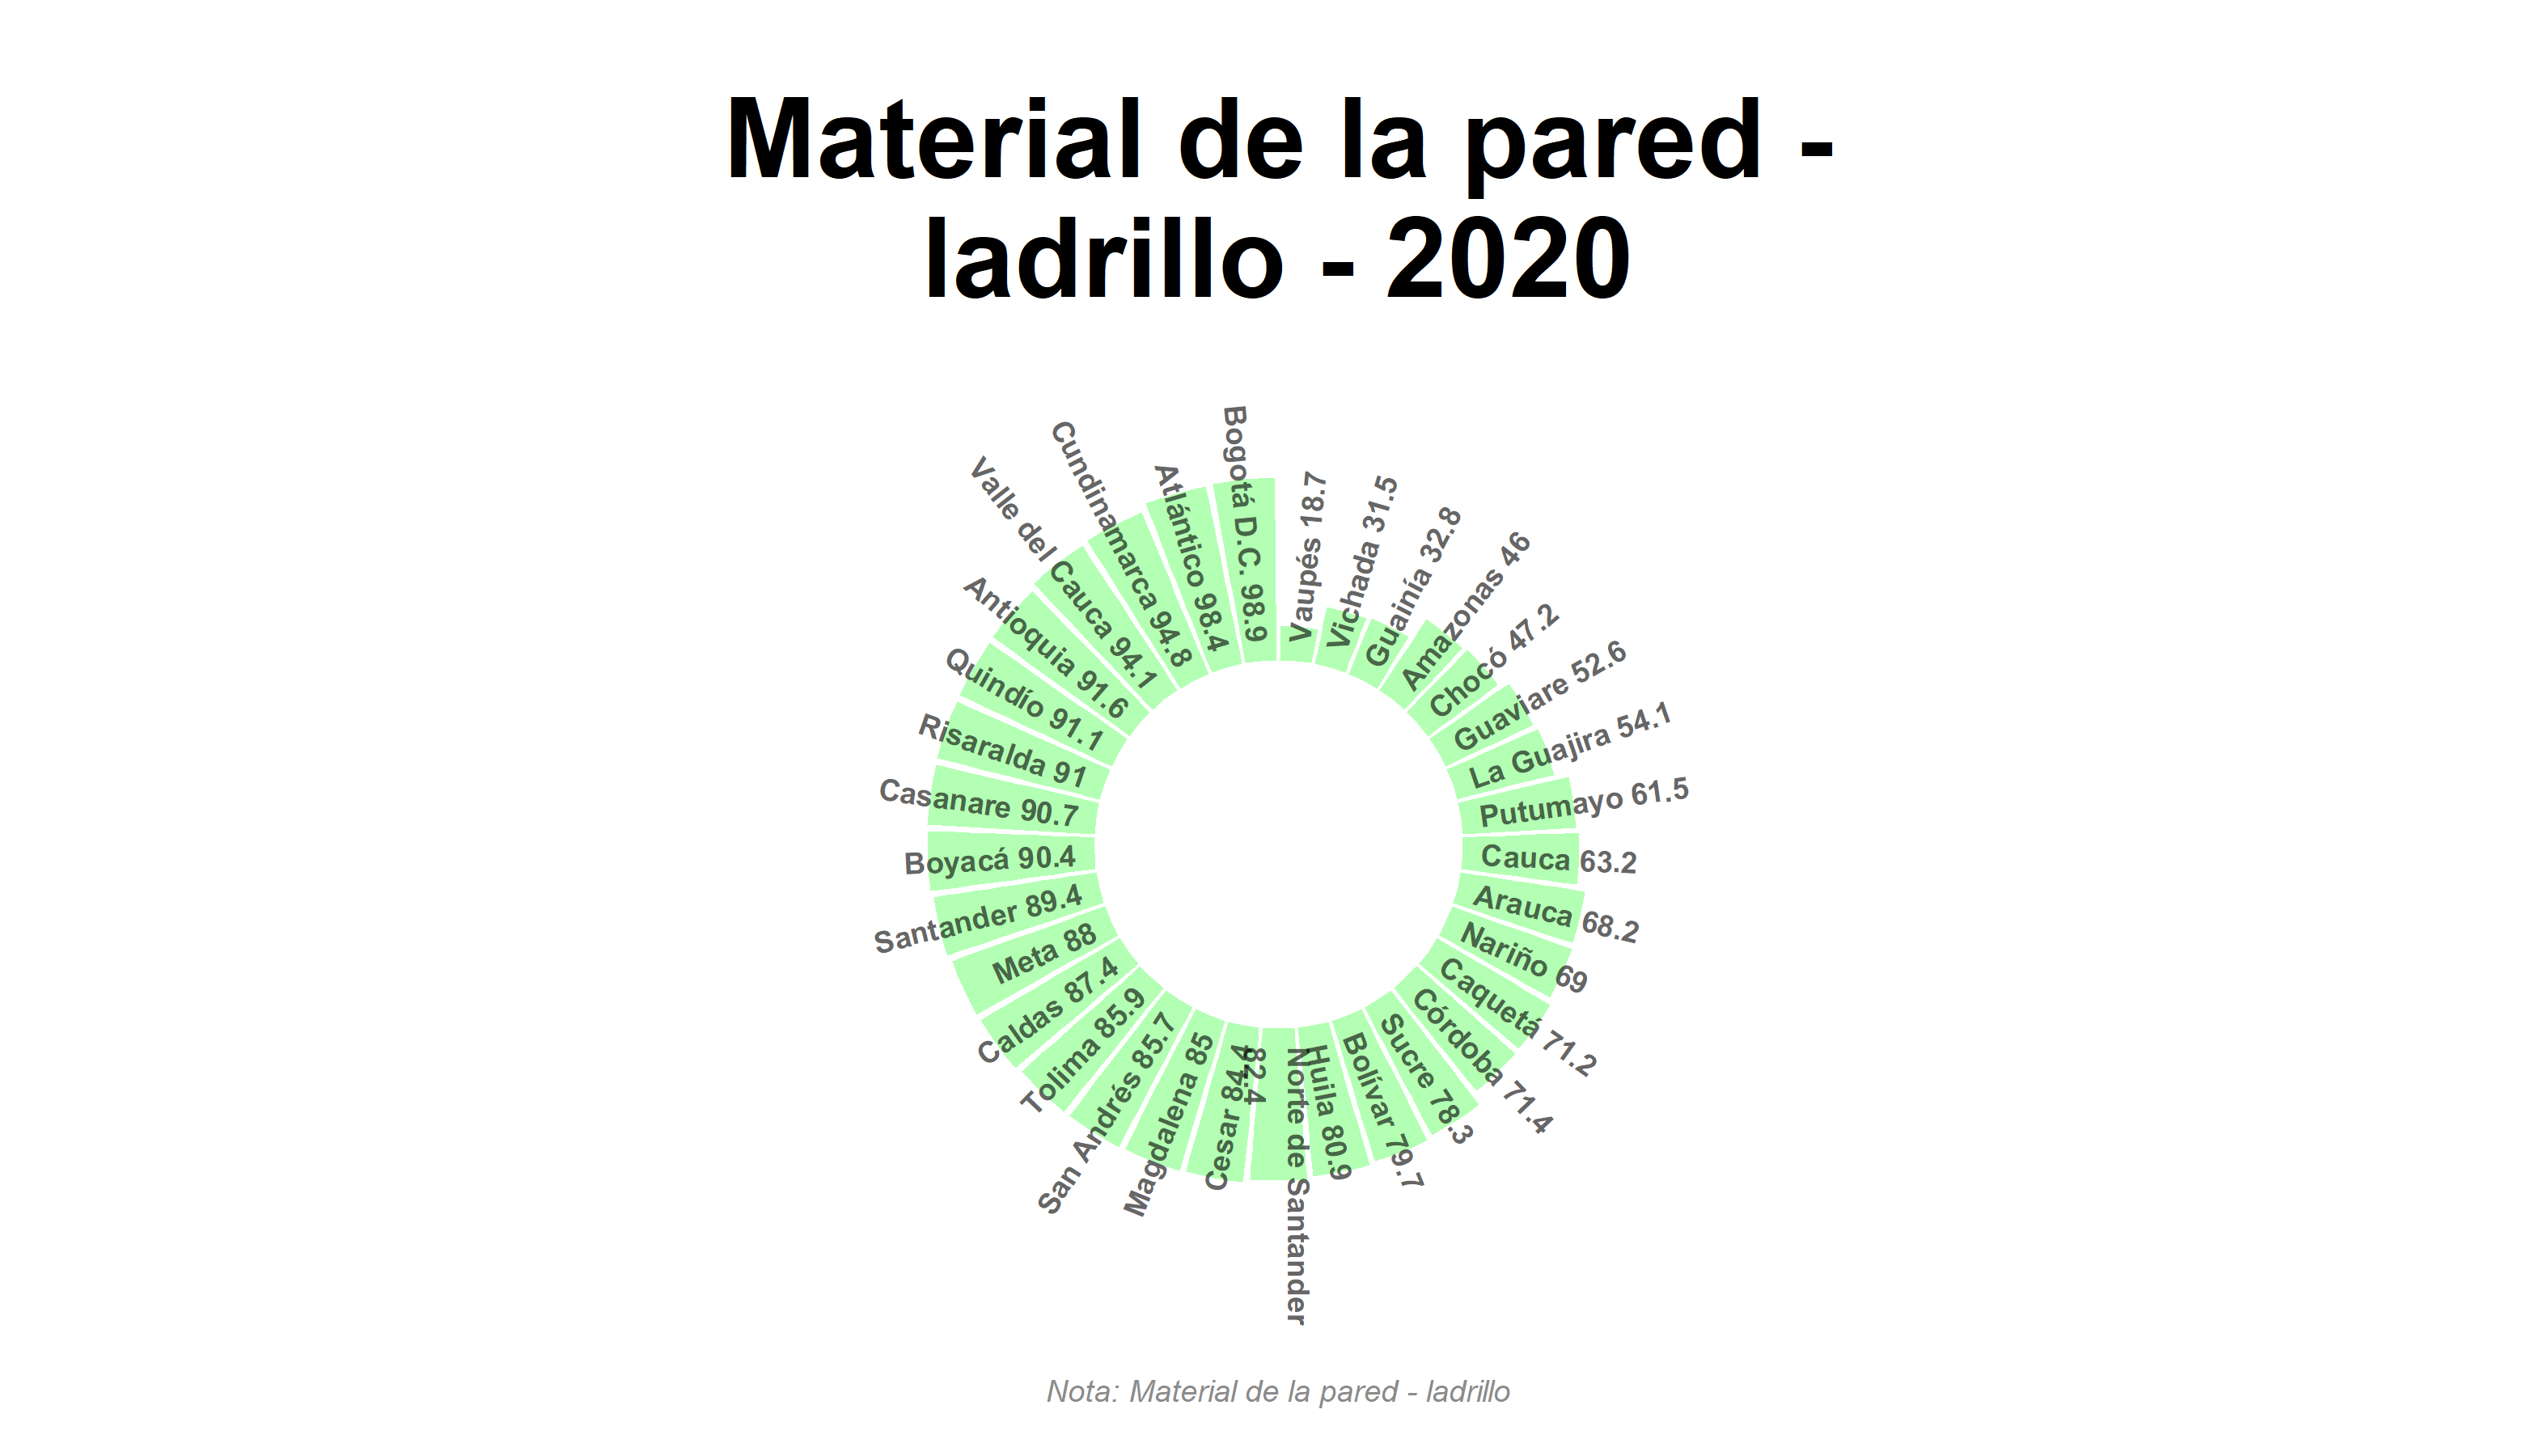
\includegraphics[width=\textwidth,keepaspectratio]{img/var_150_static.png}
        \end{center}
    \end{figure}
            \begin{itemize}
                    \item El ladrillo es el material más usado para las paredes, estando en más del 60\% de las viviendas en la mayoría de los dptos, siendo más de la mitad de estos por encima del 80\%.
                    \item La diferencia entre el territorio con más viviendas con paredes de ladrillo y el de menos es de poco más del 80\% (Bogotá - Vaupés).
                    \item Los departamentos que menos viviendas en este material tienen están por debajo del 35\%, teniendo el caso de Vaupés que solo el 19\% de las viviendas tienen paredes en este material.
                    \end{itemize}

%%%% Include figures
    \begin{figure}[H]
        \caption[Viviendas con pared de ladrillo por zonas ]{\label{pared_ladrillo_zonas} }
        \begin{center}
        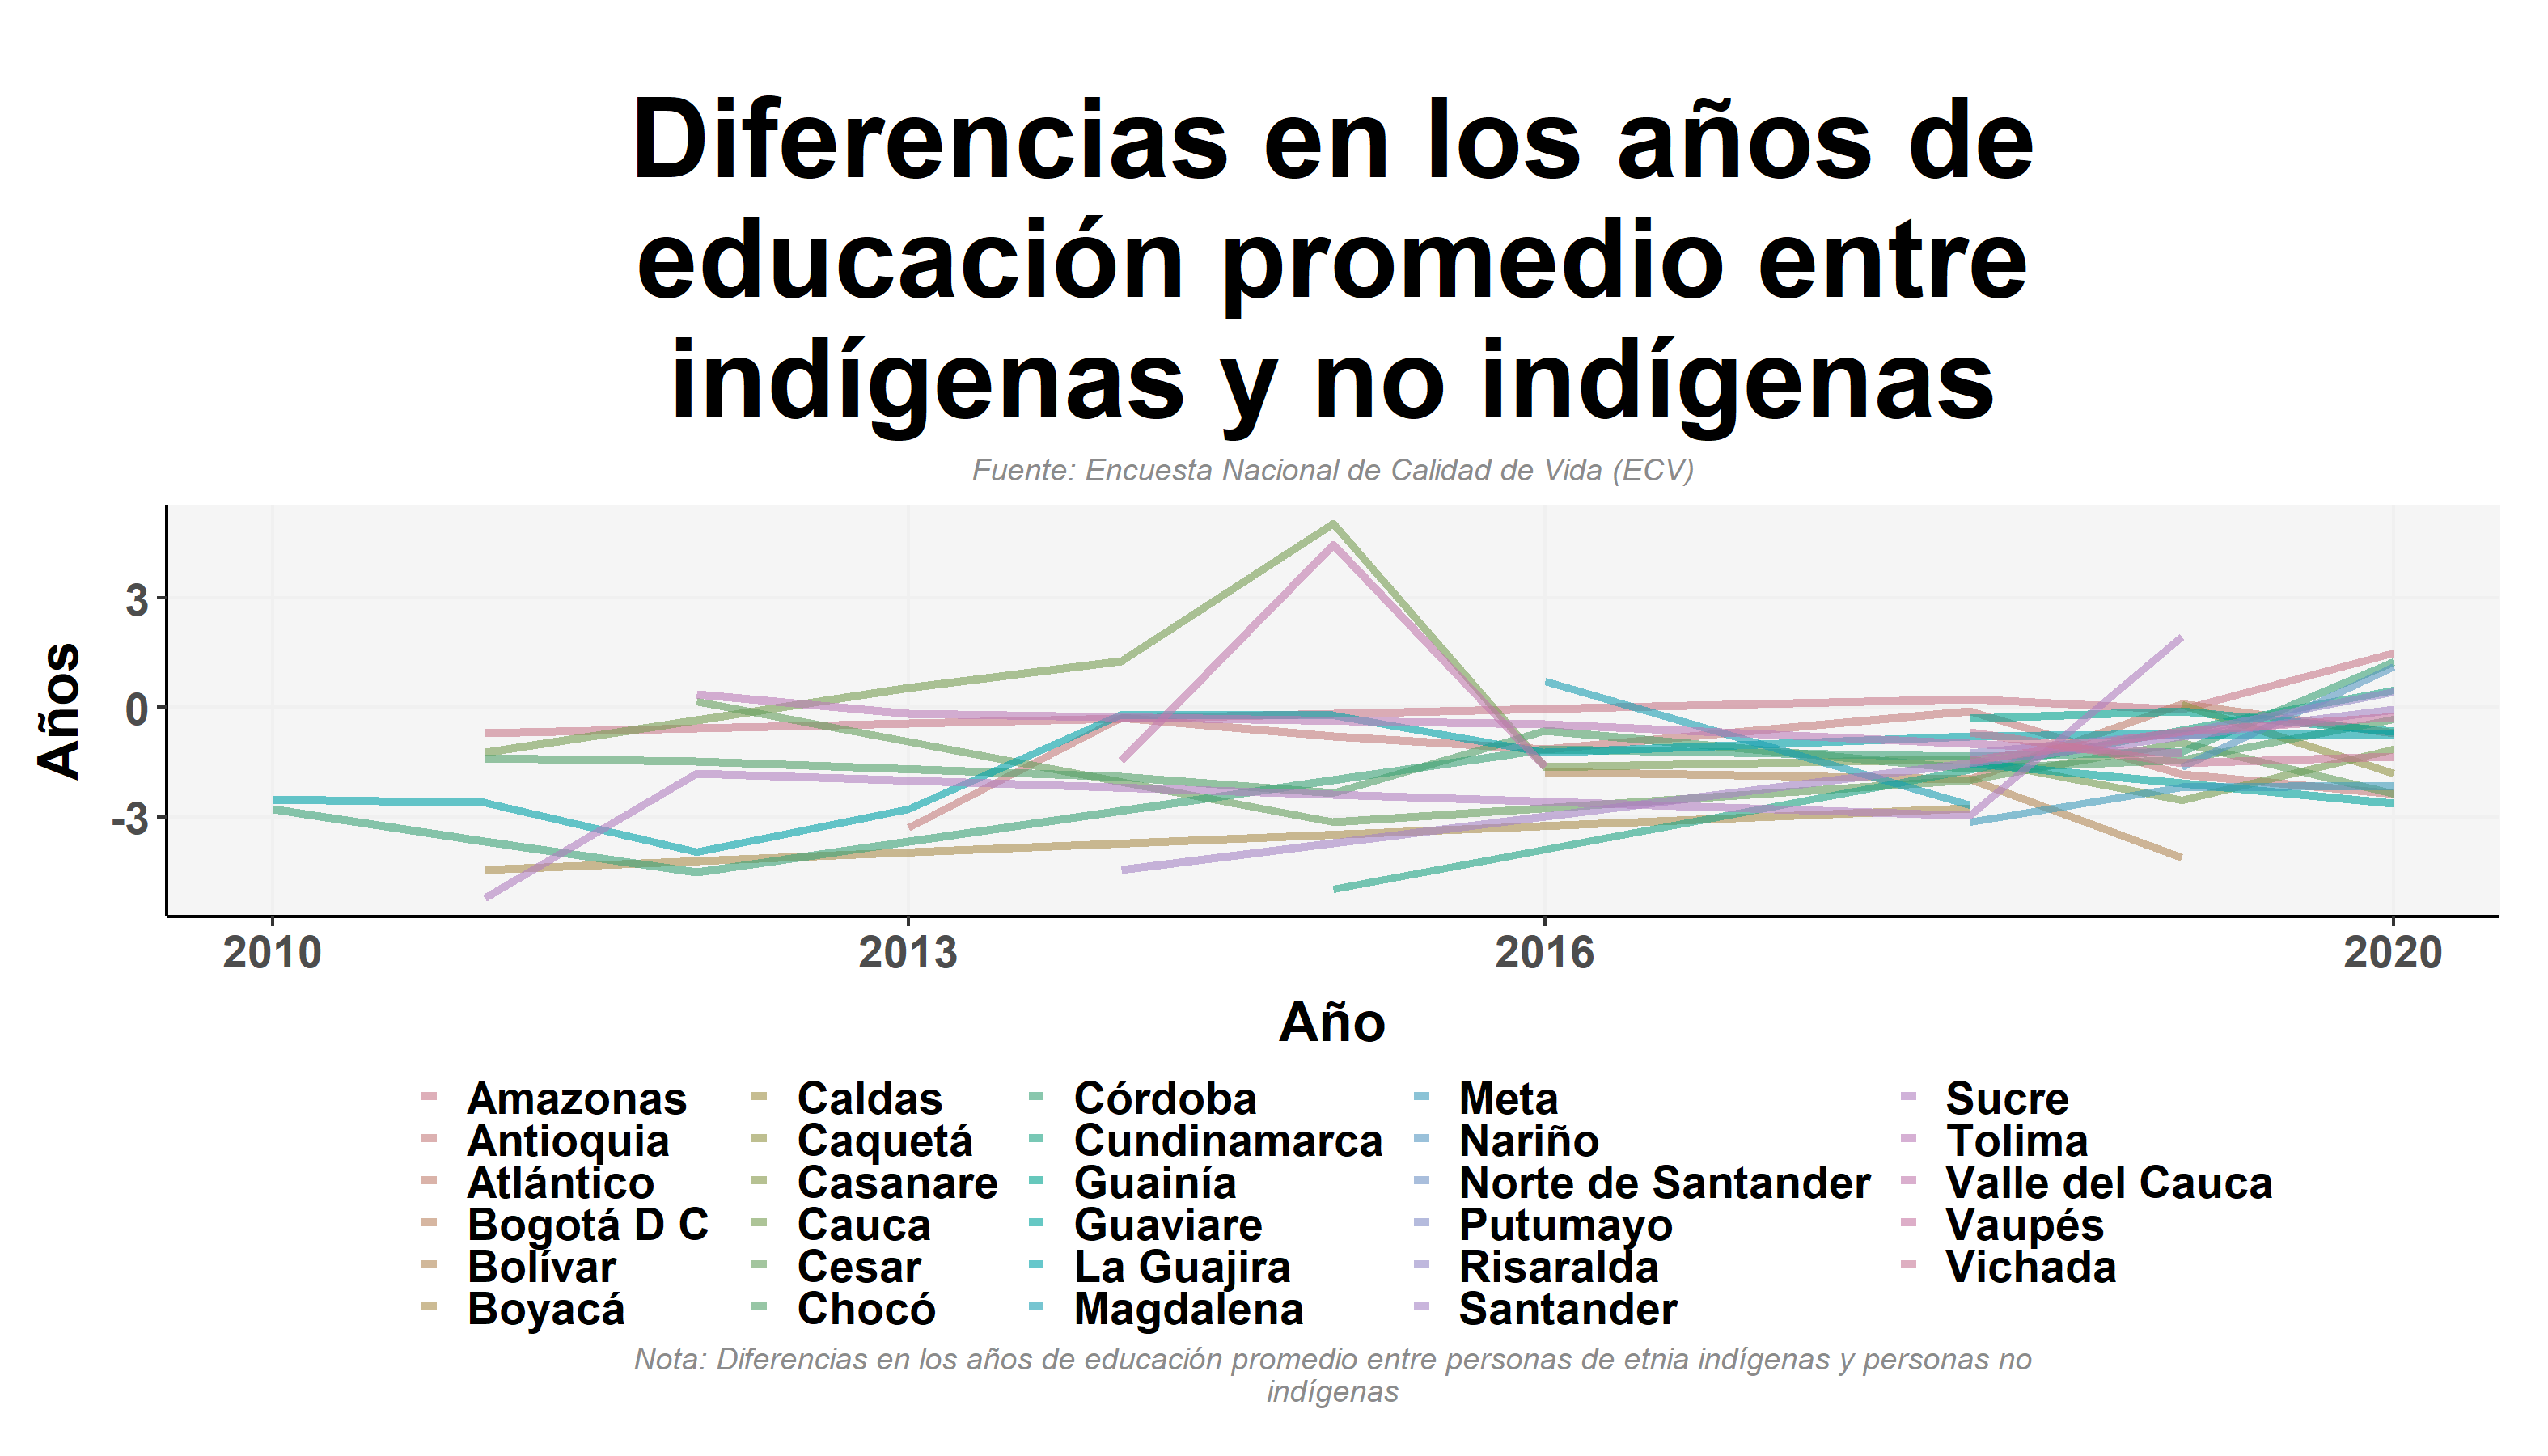
\includegraphics[width=\textwidth,keepaspectratio]{img/var_151_trend.png}
        \end{center}
    \end{figure}
            \begin{itemize}
                    \item El material es predominantemente usado en las cabeceras, estando por encima del 90\% de las viviendas, mientras que en la zona rural es cerca del 60\%.
                    \item El uso del material estaba aumentando en la zonas rurales, pero a partir del 2016 disminuyó a tal nivel que para 2020 está a los niveles que se tenían en el 2010.
                    \end{itemize}

%%%% Include figures
    \begin{figure}[H]
        \caption[Viviendas con pared de madera por departamentos para 2020 ]{\label{pared_madera_dptos} }
        \begin{center}
        \includegraphics[width=\textwidth,keepaspectratio]{img/var_160_static.png}
        \end{center}
    \end{figure}
            \begin{itemize}
                    \item Las paredes de madera son el segundo material más usado para las paredes, aunque la mitad de los territorios están por debajo del 10\% de las viviendas, los últimos cuatro están por encima del 40\%
                    \item El de menor viviendas en este material es Bogotá con menos del 1\%, mientras que el de más es Vaupés con cerca del 65\%.
                    \item La zonas en las que más se usa el materias son en la Amazonia y los llanos orientales (gráfica map 160 - 2020) con niveles por encima del 20\% de las viviendas..
                    \end{itemize}

%%%% Include figures
    \begin{figure}[H]
        \caption[Viviendas con pared de madera por zonas ]{\label{pared_madera_zonas} }
        \begin{center}
        \includegraphics[width=\textwidth,keepaspectratio]{img/var_161_trend.png}
        \end{center}
    \end{figure}
            \begin{itemize}
                    \item El material es usado predominantemente en las zonas rurales, cerca del 20\% de las viviendas, mientras que en las cabeceras está por debajo del 5\%.
                    \item El uso de este material aumentó desde 2016 para la zona rural, en las cabeceras se ha mantenido constante.
                    \end{itemize}

%%%% Include figures
    \begin{figure}[H]
        \caption[Viviendas con pared de bahareque revocado por departamentos para 2020 ]{\label{pared_bahareque_revo_dptos} }
        \begin{center}
        \includegraphics[width=\textwidth,keepaspectratio]{img/var_154_static.png}
        \end{center}
    \end{figure}
            \begin{itemize}
                    \item Aunque es el tercer material más usado encontramos que solo 3 departamentos tienen niveles por encima del 10\% de las viviendas, Huila, La Guajira y Guainía, siendo este último el de mayor con un 13.8\%.
                    \item La mitad de los departamentos tienen menos del 1\% de las viviendas, o valores cercanos a cero, con paredes en este material.
                    \end{itemize}

%%%% Include figures
    \begin{figure}[H]
        \caption[Viviendas con pared de bahareque revocado por zonas ]{\label{pared_bahareque_revo_zonas} }
        \begin{center}
        \includegraphics[width=\textwidth,keepaspectratio]{img/var_155_trend.png}
        \end{center}
    \end{figure}
            \begin{itemize}
                    \item El material es predominantemente usado en las zonas rurales, cerca de un 6\% para 2020, mientras que en las cabeceras es menos del 1\%.
                    \item El uso de este material ha venido disminuyendo en ambas zonas, pero es más notorio en el área rural, donde en 2010 estaba por encima del 8\%.
                    \end{itemize}

%%%% Include figures
    \begin{figure}[H]
        \caption[Viviendas con pared de bahareque no revocado por departamentos para 2020 ]{\label{pared_bahareque_no_revo_dptos} }
        \begin{center}
        \includegraphics[width=\textwidth,keepaspectratio]{img/var_152_static.png}
        \end{center}
    \end{figure}
            \begin{itemize}
                    \item A pesar de ser el cuarto material más usado solo 2 departamentos superan el 10\% de las viviendas con este material, Cauca y La Guajira.
                    \item Este es el segundo material más usado en La Guajira con un 29.4\%, con una diferencia de cerca del 20\% con el Cauca.
                    \end{itemize}

%%%% Include figures
    \begin{figure}[H]
        \caption[Viviendas con pared de bahareque no revocado por zonas ]{\label{pared_bahareque_no_revo_zonas} }
        \begin{center}
        \includegraphics[width=\textwidth,keepaspectratio]{img/var_153_trend.png}
        \end{center}
    \end{figure}
            \begin{itemize}
                    \item Material predominante en las zonas rurales, más del 6\% de las viviendas, en las cabeceras es cercano a cero.
                    \item A pesar que estaba disminuyendo, desde el 2016 tuvo un incremento dejándolo en 2020 con valores cercanos a los niveles del 2010.
                    \end{itemize}

%%%% Include figures
    \begin{figure}[H]
        \caption[Viviendas con pared de latas desechables por departamentos para 2020 ]{\label{pared_latas_dptos} }
        \begin{center}
        \includegraphics[width=\textwidth,keepaspectratio]{img/var_158_static.png}
        \end{center}
    \end{figure}
            \begin{itemize}
                    \item A pesar de ser uno de los materiales menos usados, se resalta que en Vaupés, Guainía y Vichada es un material bastante usado en comparación.
                    \item En el Vichada es donde más se usa, siendo que el 17.3\% de las viviendas tienen paredes en este material, superando en en poco más del 10\% a Guainía que es el segundo donde más se usa.
                    \end{itemize}

        \subsubsection{Material del Piso}

%%%% Include figures
    \begin{figure}[H]
        \caption[Viviendas con piso de baldosa por departamentos - 2010 VS 2020 ]{\label{piso_baldosa_dptos_vs} }
        \begin{center}
        \includegraphics[width=\textwidth,keepaspectratio]{img/var_173_scatter_time.png}
        \end{center}
    \end{figure}
            \begin{itemize}
                    \item Gran parte de los territorios ha aumentado el porcentaje de viviendas con este material.
                    \item Amazonas y Putumayo son los dptos que tuvieron el mayor retroceso en el porcentaje de viviendas, pasando de estar por el 60\% en 2010 a estar alrededor del 30\% en 2020.
                    \item Cauca, Huila y La Guajira presentan a 2020 niveles similares a los tenidos hace 10 años.
                    \end{itemize}

%%%% Include figures
    \begin{figure}[H]
        \caption[Viviendas con piso de baldosa por departamento para 2020 ]{\label{piso_baldosa_dptos} }
        \begin{center}
        \includegraphics[width=\textwidth,keepaspectratio]{img/var_173_static.png}
        \end{center}
    \end{figure}
            \begin{itemize}
                    \item Más de la mitad de los departamentos tienen menos del 50\% de las viviendas con pisos de baldosa.
                    \item La diferencia entre los territorios extremos es de poco más del 70\% (Bogotá - Vaupés).
                    \item A pesar de ser el material más usado en el piso se denota que la distribución varía mucho entre los territorios yendo desde 6\% hasta el 80\% de las viviendas.
                    \end{itemize}

%%%% Include figures
    \begin{figure}[H]
        \caption[Viviendas con piso de baldosa por zonas ]{\label{piso_baldosa_zonas} }
        \begin{center}
        \includegraphics[width=\textwidth,keepaspectratio]{img/var_174_trend.png}
        \end{center}
    \end{figure}
            \begin{itemize}
                    \item El uso del material para el piso de las viviendas ha aumentado, siendo más significativo en las cabeceras.
                    \item Poco más del 70\% de las viviendas en las cabeceras tienen pisos de baldosa, mientras que en las zonas rurales son el 20\% aproximadamente.
                    \end{itemize}

%%%% Include figures
    \begin{figure}[H]
        \caption[Viviendas con piso de cemento por departamentos - 2010 VS 2020 ]{\label{piso_cemento_dptos_vs} }
        \begin{center}
        \includegraphics[width=\textwidth,keepaspectratio]{img/var_177_scatter_time.png}
        \end{center}
    \end{figure}
            \begin{itemize}
                    \item Solo Santander, Putumayo y Huila presentan un incremento en el porcentaje de viviendas con pisos de cementos.
                    \item La gran mayoría de los dptos han disminuido las viviendas con este material, estando concentradas por debajo del 45\% para 2020.
                    \item Boyacá mantiene sus niveles de viviendas con pisos de cementos que tenía en el 2010.
                    \end{itemize}

%%%% Include figures
    \begin{figure}[H]
        \caption[Viviendas con piso de cemento por departamentos para 2020 ]{\label{piso_cemento_dptos} }
        \begin{center}
        \includegraphics[width=\textwidth,keepaspectratio]{img/var_177_static.png}    
        \end{center}
    \end{figure}
            \begin{itemize}
                    \item Más de la mitad de los territorios están por debajo del 40\% de viviendas con piso en cemento.
                    \item El material es el segundo más usado, teniendo una distribución amplia, desde un 6\% hasta un 57\%.
                    \item La diferencia entre los territorios extremos es de aproximadamente un 50\% (Bogotá - Caquetá).
                    \item Los dptos donde el número de viviendas con este tipo de material es mayor se encuentran especialmente en la costa, en zonas de frontera o al sur del país. Los territorios en el centro tienden a reportar menores niveles.
                    \end{itemize}

%%%% Include figures
    \begin{figure}[H]
        \caption[Viviendas con piso de cemento por zonas ]{\label{piso_cemento_zonas} }
        \begin{center}
        \includegraphics[width=\textwidth,keepaspectratio]{img/var_178_trend.png}
        \end{center}
    \end{figure}
            \begin{itemize}
                    \item En general se puede ver que en ambas zonas hay una disminución de las viviendas con piso de cemento.
                    \item El uso de cemento como material para el piso es predominante en las zonas rurales, poco más del 50\% para 2020, mientras que en las cabeceras está cercano al 20\% de las viviendas.
                    \end{itemize}

%%%% Include figures
    \begin{figure}[H]
        \caption[Viviendas con piso de tierra por departamentos - 2010 VS 2020 ]{\label{piso_tierra_dptos_vs} }
        \begin{center}
        \includegraphics[width=\textwidth,keepaspectratio]{img/var_179_scatter_time.png}
        \end{center}
    \end{figure}
            \begin{itemize}
                    \item Se denota como gran parte de los departamentos están concentrados en valores inferiores al 10\% y mantenidos entre los dos años de referencia. 
                    \item La Guajira y Arauca destacan al presentar el doble de viviendas con piso de tierra en 2020 comparada con las del 2010.
                    \item Por el lado de Córdoba y Magdalena se ve como han disminución notable en cuanto a viviendas con pisos de tierra.
                    \end{itemize}

%%%% Include figures
    \begin{figure}[H]
        \caption[Viviendas con piso de tierra por departamentos para 2020 ]{\label{piso_tierra_dptos} }
        \begin{center}
        \includegraphics[width=\textwidth,keepaspectratio]{img/var_179_static.png}
        \end{center}
    \end{figure}
            \begin{itemize}
                    \item Los extremos entre el de menor y mayor porcentaje de viviendas es avismal, teniendo a San Andrés con el 0.3\% de viviendas con piso de tierra, mientras que en el Vichada son el 66.4\% de estas, es decir que más de la mitad de las viviendas están en esta condición.
                    \item Más de la mitad de los dptos están por debajo del 10\%.
                    \item Los dptos con mayor nivel de viviendas con este tipo de piso se encuentran principalmente en la costa Caribe y en el oriente, mientras que los de menor están en la zona cafetera (gráfica map 179 para 2020).
                    \end{itemize}

%%%% Include figures
    \begin{figure}[H]
        \caption[Viviendas con piso de tierra por zonas ]{\label{piso_tierra_zonas} }
        \begin{center}
        \includegraphics[width=\textwidth,keepaspectratio]{img/var_180_trend.png}
        \end{center}
    \end{figure}
            \begin{itemize}
                    \item En las zonas rurales los pisos de tierra se presentan alrededor en el 20\% de las viviendas, mientras que en las cabeceras es menos del 3\%.
                    \item En las zonas rurales a pesar de que a principios de la década estaban disminuyendo las viviendas con este tipo de piso, desde el 2015 esta ha venido aumentan, teniendo para 2020 niveles superiores a los reportados en 2010.
                    \item Para las cabeceras las viviendas con este tipo de material han disminuido, pero aun se mantienen cerca al mismo nivel que hace 10 años.
                    \end{itemize}

%%%% Include figures
    \begin{figure}[H]
        \caption[Viviendas con piso de madera burda por departamentos - 2010 VS 2020 ]{\label{piso_madera_burda_dptos_vs} }
        \begin{center}
        \includegraphics[width=\textwidth,keepaspectratio]{img/var_175_scatter_time.png}
        \end{center}
    \end{figure}
            \begin{itemize}
                    \item La mayoría de los dptos se encuentran concentrados en cero o cerca a este.
                    \item Amazonas y Chocó son los departamentos que más aumentaron las viviendas con este tipo de pisos, triplicando y doblando, respectivamente, los valores presentados en 2010.
                    \item Caquetá y Caldas tuvieron las mayores mejoras, siendo la primera la mitad de lo que presentó en 2010.
                    \item Nariño mantiene los niveles que tenía hace 10 años.
                    \end{itemize}

%%%% Include figures
    \begin{figure}[H]
        \caption[Viviendas con piso de madera burda por departamentos para 2020 ]{\label{piso_madera_burda_dptos} }
        \begin{center}
        \includegraphics[width=\textwidth,keepaspectratio]{img/var_175_static.png}
        \end{center}
    \end{figure}
            \begin{itemize}
                    \item Solo 6 dptos presentan más del 10\% de las viviendas con pisos de este material.
                    \item Los últimos 3 dptos tienen valores alrededor del 40\%, Vaupés, Chocó y Amazonas.
                    \item Amazonas tiene casi la mitad de las viviendas con piso de madera burda, siendo este el dpto con más porcentaje, mientras que La Guajira presenta el 0.2\% de las viviendas con pisos de este material.
                    \end{itemize}

%%%% Include figures
    \begin{figure}[H]
        \caption[Viviendas con piso de madera burda por zonas ]{\label{piso_madera_burda_zonas} }
        \begin{center}
        \includegraphics[width=\textwidth,keepaspectratio]{img/var_176_trend.png}
        \end{center}
    \end{figure}
            \begin{itemize}
                    \item Para las cabeceras se ha mantenido el porcentaje de viviendas con este tipo de piso en alrededor del 2\%, con una leve disminución en el tiempo.
                    \item Para la zona rural el porcentaje de viviendas se mantuvo constante la primera mitad de la década, pero después del 2016 aumentó, mostrando para 2020 niveles superiores a los registrados en 2012.
                    \end{itemize}

        \subsubsection{Hacinamiento}

%%%% Include figures
    \begin{figure}[H]
        \caption[Hacinamiento por departamentos - Cambio porcentual entre 2018 y 2020 ]{\label{hacinamiento_dptos_cambio} }
        \begin{center}
        \includegraphics[width=\textwidth,keepaspectratio]{img/var_265_map_change.png}
        \end{center}
    \end{figure}
            \begin{itemize}
                    \item Los dptos de Chocó, Putumayo, Córdoba, Bolívar, Boyacá, Guainía y Meta presentaron una disminución del hacinamiento crítico de más del 20\%.
                    \item Por otro lado Quindío, Tolima, Huila, Bogotá, Guaviare y Vaupés fueron lo que más aumentaron los niveles de hacinamiento crítico.
                    \end{itemize}

%%%% Include figures
    \begin{figure}[H]
        \caption[Hacinamiento por departamentos para 2020 ]{\label{hacinamiento_dptos} }
        \begin{center}
        \includegraphics[width=\textwidth,keepaspectratio]{img/var_265_static.png}
        \end{center}
    \end{figure}
            \begin{itemize}
                    \item La distribución de los valores va desde 3\% hasta poco más del 30\%.
                    \item Los territorios con mayor hacinamiento crítico se ubican en la zona Caribe y el oriente - Amazonia (gráfica mas 265 para 2020).
                    \item Más de la mitad de los dptos tiene niveles por debajo del 10\% de hacinamiento crítico.
                    \item La diferencia entre el territorio con menor y mayor para 2020 nivel de hacinamiento es de cerca al 30\% (Boyacá - Vaupés).
                    \end{itemize}

%%%% Include figures
    \begin{figure}[H]
        \caption[Hacinamiento por zonas y nacional ]{\label{hacinamiento_zonas} }
        \begin{center}
        \includegraphics[width=\textwidth,keepaspectratio]{img/var_267_trend.png}
        \end{center}
    \end{figure}
            \begin{itemize}
                    \item Tanto las zonas como a nivel nacional hay una tendencia a la baja en el hacinamiento crítico, teniendo menores niveles para 2020 comparados con los reportados en 2010.
                    \item Para 2019 se ve un pico pronunciado en las cabeceras y a nivel nacional, pero en las zonas rurales este siguió a la baja en ese año.
                    \item La brecha entre las zonas rurales y cabeceras a pesar de haber disminuido, siendo el hacinamiento menor en las zonas rurales, a partir del 2019 aumentó significativamente, llevando a tener la brecha similar al 2013, un retroceso de 7 años.
                    \end{itemize}

\section{Acceso a servicios de agua potable y saneamiento}

\begin{figure}[H]
        \caption[Indicador Pulso Social sobre Acceso a servicios de agua potabla y saneamiento (PCA)]{\label{pca_pobreza} }
        \begin{center}
        \includegraphics[width=\textwidth,keepaspectratio]{pca_clusters/pca_acceso_a_servicio_de_agua_potable_y_saneamiento_pca.png}
        \end{center}
    \end{figure}

 %%%%---------------------
    %%% Principales resultados
    %%%%---------------------
    \begin{tcolorbox}[enhanced, colback=mycolor,colframe=mycolor,drop fuzzy shadow,watermark color=white,
                        %%% Título
                        title=Principales Resultados]
    
                    \begin{itemize}
                    \item Pero hay una brecha de género enorme, especialmente en los percentiles más bajos de ingreso.
                    \item El rezago en el ingreso de las mujeres con respecto al de los hombres es de más de 10 años.
                \end{itemize}
     
    \end{tcolorbox}
    %%%%---------------------
    %%%%---------------------
    %%%%---------------------
    
    
    \subsection{Agua Potable}

%%%% Include figures
    \begin{figure}[H]
        \caption[Acueducto público como fuentes de agua por departamentos - 2010 VS 2020 ]{\label{cueducto_publico_dptos_vs} }
        \begin{center}
        \includegraphics[width=\textwidth,keepaspectratio]{img/var_129_scatter_time.png}
        \end{center}
    \end{figure}
            \begin{itemize}
                    \item Es la fuente de agua más común en el país, siendo para la mayoría de los dptos más del 50\% de las viviendas usan esta fuente.
                    \item En general para 2020 la mayoría de los dptos han mejorado o mantenido los niveles que presentaron en 2010.
                    \item Chocó es el que presenta el mayor cambio entre lo años, pasando de que más del 60\% de las viviendas tengan esta fuente de agua en 2010, a manos del 25\% de las viviendas en el 2020.
                    \end{itemize}

%%%% Include figures
    \begin{figure}[H]
        \caption[Acueducto público como fuentes de agua por departamentos para 2020 ]{\label{cueducto_publico_dptos} }
        \begin{center}
        \includegraphics[width=\textwidth,keepaspectratio]{img/var_129_static.png}
        \end{center}
    \end{figure}
            \begin{itemize}
                    \item Aunque más de la mitad de los territorios tienen como fuente de agua el acueducto público en más del 60\% de las viviendas, también hay zonas con menos del 20\%.
                    \item Bogotá es el territorio con más viviendas con esta fuente de agua, 98.9\%, mientras que Vaupés presenta el menor número con un 0.8\%.
                    \item Las zonas de menor acceso a esta fuente de agua se encuentran ubicadas en la región de la Amazonia y los llanos orientales, y el Chocó (map 129 2020).
                    \end{itemize}

%%%% Include figures
    \begin{figure}[H]
        \caption[Acueducto público como fuentes de agua por zonas ]{\label{cueducto_publico_zonas} }
        \begin{center}
        \includegraphics[width=\textwidth,keepaspectratio]{img/var_130_trend.png}
        \end{center}
    \end{figure}
            \begin{itemize}
                    \item Mientras que en las cabeceras más del 90\% de las viviendas tienen acceso a un acueducto público, en las zonas rurales es cerca del 20\%.
                    \item En el trascurso de los años el porcentaje de viviendas con acceso a un acueducto público se ha mantenido en valores similares, sin mayores cambios desde el 2010.
                    \end{itemize}

%%%% Include figures
    \begin{figure}[H]
        \caption[Acueducto comunal como fuentes de agua por departamentos - 2010 VS 2020 ]{\label{cueducto_comunal_dptos_vs} }
        \begin{center}
        \includegraphics[width=\textwidth,keepaspectratio]{img/var_133_scatter_time.png}
        \end{center}
    \end{figure}
            \begin{itemize}
                    \item Aunque en la mayoría de los dptos ha aumentado las viviendas con el acceso a esta fuente de agua, gran parte se concentra por debajo del 20\%.
                    \item Meta, Nariño, Risaralda y Caldas son los dptos donde más disminuyó el acceso a esta fuente de agua entre los años de referencia.
                    \end{itemize}

%%%% Include figures
    \begin{figure}[H]
        \caption[Acueducto comunal como fuentes de agua por departamentos para 2020 ]{\label{cueducto_comunal_dptos} }
        \begin{center}
        \includegraphics[width=\textwidth,keepaspectratio]{img/var_133_static.png}
        \end{center}
    \end{figure}
            \begin{itemize}
                    \item Se encuentra que para 2020 el 75\% de los territorios tienen menos del 15\% de las viviendas con acceso a un acueducto comunal.
                    \item Hay territorio que no tienen acueducto comunal, San Andrés y Vaupés, siendo los de menor rango, mientras que Boyacá, Nariño y Cauca tienen alrededor de un 30\% de las viviendas que dependen de esta fuente de agua, siendo el de mayor porcentaje Cauca con un 34.5\%.
                    \item Esta fuente de agua se concentra en el 2020 en la zona centro y sur-occidente del país (map 133 2020)
                    \end{itemize}

%%%% Include figures
    \begin{figure}[H]
        \caption[Acueducto comunal como fuentes de agua por zonas ]{\label{cueducto_comunal_zonas} }
        \begin{center}
        \includegraphics[width=\textwidth,keepaspectratio]{img/var_134_trend.png}
        \end{center}
    \end{figure}
            \begin{itemize}
                    \item El acueducto tiene un papel protagónico en los centros poblados y rural disperso, siendo la fuente de agua para cerca del 40\% de las viviendas, mientras que en las cabeceras son menos del 5\% de las viviendas.
                    \item Para la zona rural vemos que ha sido muy variada en los años, y aunque a finales de la década estaba disminuyendo, para 2020 aumentó superando los valores del 2010.
                    \end{itemize}

%%%% Include figures
    \begin{figure}[H]
        \caption[Río o quebradas como fuentes de agua por departamentos - 2010 VS 2020 ]{\label{rio_dptos_vs} }
        \begin{center}
        \includegraphics[width=\textwidth,keepaspectratio]{img/var_142_scatter_time.png}
        \end{center}
    \end{figure}
            \begin{itemize}
                    \item Es la tercera fuente de agua más usada por las viviendas aunque gran parte de los territorios está concentrada por debajo del 10\% y la mayoría tuvieron mejoras entre el 2010 y 2020.
                    \item Algunos dptos no están dado que se tuvieron en cuenta en la ECV desde 2018.
                    \end{itemize}

%%%% Include figures
    \begin{figure}[H]
        \caption[Río o quebradas como fuentes de agua por departamentos para 2020 ]{\label{rio_dptos} }
        \begin{center}
        \includegraphics[width=\textwidth,keepaspectratio]{img/var_141_static.png}
        \end{center}
    \end{figure}
            \begin{itemize}
                    \item Todos los dptos están por debajo del 20\%, incluso más del 75\% de estos están por debajo del 10\%, pero hay uno que es el de mayor porcentaje, Vichada, donde cerca del 60\% de las viviendas su fuente de agua es un río o una quebrada.
                    \item Los dptos que más usan esta fuente de agua se encuentran principalmente en la zona oriental y amazónica (map 141 2020)
                    \end{itemize}

%%%% Include figures
    \begin{figure}[H]
        \caption[Río o quebradas como fuentes de agua por zonas ]{\label{rio_zonas} }
        \begin{center}
        \includegraphics[width=\textwidth,keepaspectratio]{img/var_142_trend.png}
        \end{center}
    \end{figure}
            \begin{itemize}
                    \item Es principalmente usada en las zonas rurales, alrededor del 15\%.
                    \item Para las cabeceras el uso de esta fuente agua es cercano a cero.
                    \item En los últimos años a disminuido el uso de esta fuente de en la zona rural, mostrando valores menores en 2020 a los registrados en el 2010.
                    \end{itemize}

%%%% Include figures
    \begin{figure}[H]
        \caption[Pozo con bomba como fuentes de agua por departamentos - 2010 VS 2020 ]{\label{pozo_bomba_dptos_vs} }
        \begin{center}
        \includegraphics[width=\textwidth,keepaspectratio]{img/var_135_scatter_time.png}
        \end{center}
    \end{figure}
            \begin{itemize}
                    \item Aunque en la mayoría de los dptos no es una fuente de agua muy utilizada, tenemos casos como Casanare y Arauca que pasaron de 0\% de viviendas con esta fuente, a más del 10\%, incluso del 20\% para Arauca.
                    \item En zonas como Amazonas, Bolívar, Putumayo y Magdalena el porcentaje de viviendas con esta fuente de agua disminuyó.
                    \end{itemize}

%%%% Include figures
    \begin{figure}[H]
        \caption[Pozo con bomba como fuentes de agua por departamentos para 2020 ]{\label{pozo_bomba_dptos} }
        \begin{center}
        \includegraphics[width=\textwidth,keepaspectratio]{img/var_135_static.png}
        \end{center}
    \end{figure}
            \begin{itemize}
                    \item Menos del 10\% de las viviendas en el 75\% de los territorios usan el pozo con bomba como fuente de agua.
                    \item Los últimos cuatro dptos tienen por encima del 20\% de las viviendas con esta fuente de agua. Se destaca que los dptos hacen parte de la zona oriental y amazónica del país, donde es popular esta fuente de agua (map 135 2020).
                    \item Guainía es el dpto con mayor proporción de viviendas con esta fuente de agua, 37.1\%, mientras que Bogotá presenta el menor, con cero viviendas, seguido por Caldas con el 0.1\%.
                    \end{itemize}

%%%% Include figures
    \begin{figure}[H]
        \caption[Pozo con bomba como fuentes de agua por zonas ]{\label{pozo_bomba_zonas} }
        \begin{center}
        \includegraphics[width=\textwidth,keepaspectratio]{img/var_136_trend.png}
        \end{center}
    \end{figure}
            \begin{itemize}
                    \item Es una fuente de agua utilizada especialmente en la zona rural que ha venido en aumento presentando para 2020 valores superiores a los del 2010, aunque en el 2020 hubo una disminución de este.
                    \item Para la cabeceras estás son menos del 1 \%. de las viviendas y se ha mantenido constante.
                    \end{itemize}

%%%% Include figures
    \begin{figure}[H]
        \caption[Agua lluvia como fuentes de agua por departamentos - 2010 VS 2020 ]{\label{agua_lluvia_dptos_vs} }
        \begin{center}
        \includegraphics[width=\textwidth,keepaspectratio]{img/var_139_scatter_time.png}
        \end{center}
    \end{figure}
            \begin{itemize}
                    \item Es una fuente de agua poco común donde la mayoría de los territorios menos del 5\% de las viviendas la usas, pero en territorios como Chocó se duplicó aproximadamente las viviendas que usan esta fuente de agua, o el Amazonas donde pasó de reportar niveles cercanos a cero en 2010 a más del 30\% en el 2020.
                    \item Córdoba pasó de tener poco más del 30\% de las viviendas teniendo como fuente de agua la lluvia en 2010 a niveles cercanos a cero en el 2020, Putumayo y Magdalena también presentaron cambios similares.
                    \end{itemize}

%%%% Include figures
    \begin{figure}[H]
        \caption[Agua lluvia como fuentes de agua por departamentos para 2020 ]{\label{agua_lluvia_dptos} }
        \begin{center}
        \includegraphics[width=\textwidth,keepaspectratio]{img/var_139_static.png}
        \end{center}
    \end{figure}
            \begin{itemize}
                    \item Más del 75\% de los territorios tienen menos del 10\% de las viviendas con el agua lluvia como fuente de agua.
                    \item Vaupés y Chocó son los dptos con mayor viviendas con esta fuente de agua, siendo el 84.6\% y 70.4\% de las viviendas respectivamente, a esto también se le unen dptos como Amazonas y Guainía pero con valores entre 20 y 30\% aproximadamente.
                    \item Los dptos con mayor uso de esta fuente de agua se encuentran en el sur y occidente del país (map 139 2020).
                    \end{itemize}

%%%% Include figures
    \begin{figure}[H]
        \caption[Agua lluvia como fuentes de agua por zonas ]{\label{agua_lluvia_zonas} }
        \begin{center}
        \includegraphics[width=\textwidth,keepaspectratio]{img/var_140_trend.png}
        \end{center}
    \end{figure}
            \begin{itemize}
                    \item Es una fuente de agua especialmente usada en las zonas rurales, estando alrededor del 6\% de las viviendas.
                    \item Para las cabeceras esta ha estado disminuyendo hasta niveles por debajo del 1\%.
                    \item En ambas zonas se registraron valores menores en 2020 comparados con los de 2010.
                    \end{itemize}

%%%% Include figures
    \begin{figure}[H]
        \caption[Pozo sin bomba como fuentes de agua por departamentos para 2020 ]{\label{pozo_no_bomba_dptos} }
        \begin{center}
        \includegraphics[width=\textwidth,keepaspectratio]{img/var_137_static.png}
        \end{center}
    \end{figure}
            \begin{itemize}
                    \item Se resalta que para La Guajira y Putumayo el 30.2\% y el 21.9\% de las viviendas respectivamente usan el pozo sin bomba como fuente de agua.
                    \item Para los demás dptos, poco más del 75\% de ellos, son menos del 5\% de las viviendas lo usan como fuente de agua.
                    \end{itemize}

%%%% Include figures
    \begin{figure}[H]
        \caption[Agua en botella o bolsa como fuentes de agua por departamentos para 2020 ]{\label{agua_botella_dptos} }
        \begin{center}
        \includegraphics[width=\textwidth,keepaspectratio]{img/var_143_static.png}
        \end{center}
    \end{figure}
            \begin{itemize}
                    \item Para San Andrés el agua en botella o en bolsa es una de las principales fuentes de agua, siendo esta para el 41.1\% de las viviendas en el dpto. Vaupés le sigue con el 12.3\% de las viviendas.
                    \item A excepción de los dptos mencionados anteriormente los demás territorios están por debajo del 10\%, incluso la mayoría está por debajo del 3\%.
                    \end{itemize}

%%%% Include figures
    \begin{figure}[H]
        \caption[Carrotanque como fuentes de agua por departamentos para 2020 ]{\label{carrotanque_dptos} }
        \begin{center}
        \includegraphics[width=\textwidth,keepaspectratio]{img/var_147_static.png}
        \end{center}
    \end{figure}
            \begin{itemize}
                    \item Es de las fuentes de agua menos común en el país, donde cerca del 80\% son menos del 1\%, pero se destaca que en La Guajira el 10.4\% de las viviendas tienen como fuente de agua el carrotanque.
                    \end{itemize}

    \subsection{Saneamiento}

%%%% Include figures
    \begin{figure}[H]
        \caption[Saneamiento dentro de la vivienda por departamentos - 2010 VS 2020 ]{\label{saneamiento_dentro_dptos_vs} }
        \begin{center}
        \includegraphics[width=\textwidth,keepaspectratio]{img/var_193_scatter_time.png}
        \end{center}
    \end{figure}
            \begin{itemize}
                    \item Gran parte de los territorios están concentrados por encima del 75\% de las viviendas, además de que en general el saneamiento al interior de las viviendas ha aumentado entre 2010 y 2020.
                    \item Arauca, Putumayo y Amazonas muestran un gran retroceso en el porcentaje de viviendas con el saneamiento en el interior, pasando de valores cercanos al 80\% en 2010 a cerca del 50\% en el 2020.
                    \item Huila, Tolima y Nariño mantuvieron los niveles que tenían hace 10 años.
                    \end{itemize}

%%%% Include figures
    \begin{figure}[H]
        \caption[Saneamiento dentro de la vivienda por departamentos (mapa) - 2010 VS 2020 ]{\label{saneamiento_dentro_dptos_mapa} }
        \begin{center}
        \includegraphics[width=\textwidth,keepaspectratio]{img/var_193_map.png}
        \end{center}
    \end{figure}
            \begin{itemize}
                    \item Se ve que en el centro del país para 2020 se aumenta el porcentaje de viviendas con baño en el interior, caso contrario pasa a medida que se aleja del centro. 
                    \item Se destaca que la zonas del oriente y la Amazonia se centran los territorios con menor porcentaje de viviendas con saneamiento en el interior.
                    \end{itemize}

%%%% Include figures
    \begin{figure}[H]
        \caption[Saneamiento dentro de la vivienda por departamentos para 2020 ]{\label{saneamiento_dentro_dptos} }
        \begin{center}
        \includegraphics[width=\textwidth,keepaspectratio]{img/var_193_static.png}
        \end{center}
    \end{figure}
            \begin{itemize}
                    \item Los 3 departamentos que menos tienen viviendas con saneamiento dentro están por debajo del 30\%, mientras que más de la mitad de los territorios está por encima del 65\% de las viviendas.
                    \item Mientras que en Vaupés solo 17.9\% de las viviendas tienen el saneamiento en el interior, en Bogotá es el 98.7\% de las viviendas.
                    \end{itemize}

%%%% Include figures
    \begin{figure}[H]
        \caption[Saneamiento dentro de la vivienda por zonas ]{\label{saneamiento_dentro_zonas} }
        \begin{center}
        \includegraphics[width=\textwidth,keepaspectratio]{img/var_194_trend.png}
        \end{center}
    \end{figure}
            \begin{itemize}
                    \item En ambas zonas han aumentado las viviendas con el saneamiento en el interior, siendo este mayor en las zonas rurales.
                    \item La zona rural presenta un aumento, logrando que la zona rural pase del 50\% de las viviendas con saneamiento en el interior.
                    \end{itemize}

%%%% Include figures
    \begin{figure}[H]
        \caption[Saneamiento fuera de la vivienda por departamentos - 2010 VS 2020 ]{\label{saneamiento_fuera_dptos_vs} }
        \begin{center}
        \includegraphics[width=\textwidth,keepaspectratio]{img/var_195_scatter_time.png}
        \end{center}
    \end{figure}
            \begin{itemize}
                    \item En la mayoría de los dptos se ha disminuido las viviendas con saneamiento fuera, especialmente en el Meta, La Guajira, Cundinamarca y Casanare.
                    \item Huila y Bogotá presentan a 2020 los mismos niveles que en el 2010.
                    \item Arauca, Amazonas, Putumayo y Norte son los dptos que tuvieron un aumento significativo en las viviendas con saneamiento fuera.
                    \end{itemize}

%%%% Include figures
    \begin{figure}[H]
        \caption[Saneamiento fuera de la vivienda por departamentos (mapa) - 2010 VS 2020 ]{\label{saneamiento_fuera_mapa} }
        \begin{center}
        \includegraphics[width=\textwidth,keepaspectratio]{img/var_195_map.png}
        \end{center}
    \end{figure}
            \begin{itemize}
                    \item Caso contrario a lo que pasa con el saneamiento dentro, acá a medida que se aleja del centro aumentan las viviendas con saneamiento fuera, mientras que en el centro del país disminuyen las viviendas con este tipo de saneamiento.
                    \item La Amazonia y parte de la costa presentan los porcentajes más altos de viviendas con el saneamiento fuera.
                    \end{itemize}

%%%% Include figures
    \begin{figure}[H]
        \caption[Saneamiento fuera de la vivienda por departamentos para 2020 ]{\label{saneamiento_fuera_dptos} }
        \begin{center}
        \includegraphics[width=\textwidth,keepaspectratio]{img/var_195_static.png}
        \end{center}
    \end{figure}
            \begin{itemize}
                    \item Alrededor del 30\% de los dptos tienen menos del 10\% de las viviendas con saneamiento fuera.
                    \item Los 3 dptos con mayor porcentaje de viviendas con saneamiento están cerca del 40\%, teniendo Arauca el más alto con un 39.8\%.
                    \item Bogotá presenta el menor número de viviendas con el saneamiento fuera con un 1.3\%.
                    \end{itemize}

%%%% Include figures
    \begin{figure}[H]
        \caption[Saneamiento fuera de la vivienda por zonas ]{\label{saneamiento_fuera_zonas} }
        \begin{center}
        \includegraphics[width=\textwidth,keepaspectratio]{img/var_196_trend.png}
        \end{center}
    \end{figure}
            \begin{itemize}
                    \item Ambas zonas presentan una disminución en el porcentaje de las viviendas con el saneamiento fuera.
                    \item En las zonas rurales es más común este tipo de saneamiento estando en cerca al 30\% de las viviendas, mientras que en las cabeceras es cerca del 5\%.
                    \end{itemize}

\section{Crecimiento Económico y Productivo}

\begin{figure}[H]
        \caption[Indicador Pulso Social sobre Crecimiento Económico y Productivo]{\label{pca_pobreza} }
        \begin{center}
        \includegraphics[width=\textwidth,keepaspectratio]{pca_clusters/pca_crecimiento_economico_y_productivo_pca.png}
        \end{center}
    \end{figure}

 %%%%---------------------
    %%% Principales resultados
    %%%%---------------------
    \begin{tcolorbox}[enhanced, colback=mycolor,colframe=mycolor,drop fuzzy shadow,watermark color=white,
                        %%% Título
                        title=Principales Resultados]
    
                    \begin{itemize}
                    \item Pero hay una brecha de género enorme, especialmente en los percentiles más bajos de ingreso.
                    \item El rezago en el ingreso de las mujeres con respecto al de los hombres es de más de 10 años.
                \end{itemize}
     
    \end{tcolorbox}
    %%%%---------------------
    %%%%---------------------
    %%%%---------------------
    
    
    \subsection{Indicadores Convencionales}
        \subsubsection{Índice de diversidad económica}

%%%% Include figures
    \begin{figure}[H]
        \caption[Índice de diversidad económica por departamentos (mapa) - 2010 VS 2020 ]{\label{diversidad_econ_dptos_mapa} }
        \begin{center}
        \includegraphics[width=\textwidth,keepaspectratio]{img/var_300_map.png}
        \end{center}
    \end{figure}
            \begin{itemize}
                    \item En general se muestra como los territorios se han vuelto más diversos económicamente hablando.
                    \item Las regiones tienden a compartir el mismos niveles de diversidad económica entre los dptos que la componen.
                    \item Las regiones de los llanos orientales y la Amazonia presentan la menor diversidad económica.
                    \item Meta, Quindío, Magdalena y Córdoba muestran un aumento en el índice, es decir se hicieron menos diversos. Por otro lado Arauca, Casanare y La Guajira se volvieron significativamente más diversas (300 scatter).
                    \item La mayoría de los departamentos catalogados como menos diversos, se han mantenido con los mismos niveles que se tenían en el 2005 (300 scatter).
                    \end{itemize}

%%%% Include figures
    \begin{figure}[H]
        \caption[Índice de diversidad económica por departamentos para 2020 ]{\label{diversidad_econ_dptos} }
        \begin{center}
        \includegraphics[width=\textwidth,keepaspectratio]{img/var_300_static.png}
        \end{center}
    \end{figure}
            \begin{itemize}
                    \item Mientras que en Antioquia el índice es de 9.9, siendo el territorio con más diversidad, en Vaupés por otro lado es la zona con menor diversidad, teniendo un índice de 34.4.
                    \end{itemize}

        \subsubsection{Establecimientos}

%%%% Include figures
    \begin{figure}[H]
        \caption[Establecimientos por departamentos - Cambio porcentual entre 2009 y 2019 ]{\label{establecimientos_dptos_cambio} }
        \begin{center}
        \includegraphics[width=\textwidth,keepaspectratio]{img/var_217_map_change.png}
        \end{center}
    \end{figure}
            \begin{itemize}
                    \item Se resalta que la información no está para todos los departamentos.
                    \item En la zona centro del país se evidencia un aumento en el número de establecimientos a excepción de Bogotá que es de las zonas en donde disminuyó.
                    \item El grueso de los territorios ha disminuido el número de establecimientos entre 2009 y 2019.
                    \end{itemize}

%%%% Include figures
    \begin{figure}[H]
        \caption[Establecimientos a nivel nacional ]{\label{establecimientos_nacional} }
        \begin{center}
        \includegraphics[width=\textwidth,keepaspectratio]{img/var_218_trend.png}
        \end{center}
    \end{figure}
            \begin{itemize}
                    \item Entre 2009 y 2010 se vio un aumento en el número de establecimientos.
                    \item A partir del 2010 los establecimientos disminuyeron significativamente, pasando de tener cerca de 10mil establecimientos a nivel nacional en 2010 a reportar alrededor de 7mil en 2019.
                    \end{itemize}

        \subsubsection{Personal promedio por empresa}

%%%% Include figures
    \begin{figure}[H]
        \caption[Personal promedio por empresa por departamentos - 2009 VS 2019 ]{\label{personal_promedio_dptos_vs} }
        \begin{center}
        \includegraphics[width=\textwidth,keepaspectratio]{img/var_220_scatter_time.png}
        \end{center}
    \end{figure}
            \begin{itemize}
                    \item Gran parte de los dptos se vio un aumento en el personal promedio por empresas, siendo Cauca, Caldas y Casanare tienen el mayor aumento entre 2009 y 2019.
                    \item Cundinamarca es el único dpto que disminuye su personal promedio pero no de manera significante.
                    \end{itemize}

%%%% Include figures
    \begin{figure}[H]
        \caption[Personal promedio por empresa a nivel nacional ]{\label{personal_promedio_nacional} }
        \begin{center}
        \includegraphics[width=\textwidth,keepaspectratio]{img/var_221_trend.png}
        \end{center}
    \end{figure}
            \begin{itemize}
                    \item Aunque en el 2010 se disminuyó el promedio de personal por empresa, este ha aumentado significativamente desde entonces.
                    \item Para 2019 el personas promedio por empresa fue poco más de 90 personas, mientras que en 2009 fue de alrededor de 70 personas.
                    \end{itemize}

        \subsubsection{Producción bruta}

%%%% Include figures
    \begin{figure}[H]
        \caption[Producción bruta por departamentos (mapa) - 2009 VS 2019 ]{\label{prod_bruta_dptos_mapa} }
        \begin{center}
        \includegraphics[width=\textwidth,keepaspectratio]{img/var_223_map.png}
        \end{center}
    \end{figure}
            \begin{itemize}
                    \item En general los dptos mantienen sus niveles de producción bruta o con leves aumentos entre 2009 y 2019, especialmente para Cundinamarca, Bolívar y Santander.
                    \item La mayor producción se concentra en la zona centro del país, aunque cabe destacar que falta información de las zonas más alejadas del país (Amazonia - llanos orientales).
                    \end{itemize}

%%%% Include figures
    \begin{figure}[H]
        \caption[Producción bruta a nivel nacional ]{\label{prod_bruta_nacional} }
        \begin{center}
        \includegraphics[width=\textwidth,keepaspectratio]{img/var_224_trend.png}
        \end{center}
    \end{figure}
            \begin{itemize}
                    \item Desde 2009 estaba en aumento hasta un pico en el 2016, donde tuvo un retroceso que para el 2019 aún no se había recuperado a los niveles del pico más alto.
                    \end{itemize}

        \subsubsection{Valor agregado}

%%%% Include figures
    \begin{figure}[H]
        \caption[Valor agregado por departamentos (mapa) - 2009 VS 2019 ]{\label{valor_agreg_dptos_mapa} }
        \begin{center}
        \includegraphics[width=\textwidth,keepaspectratio]{img/var_226_map.png}
        \end{center}
    \end{figure}
            \begin{itemize}
                    \item El valor agregado a mantenido los valores similares en los territorios entre 2009 y 2019.
                    \item El valor agregado más alto se concentra en el interior del país, siendo mayor en Antioquia, Cundinamarca, Valle y Bogotá.
                    \item Los dptos con en las zonas de la Amazonia y oriente no tienen información.
                    \end{itemize}

%%%% Include figures
    \begin{figure}[H]
        \caption[Valor agregado a nivel nacional ]{\label{valor_agreg_nacional} }
        \begin{center}
        \includegraphics[width=\textwidth,keepaspectratio]{img/var_227_trend.png}
        \end{center}
    \end{figure}
            \begin{itemize}
                    \item A nivel nacional el valor agregado varía a través del tiempo, que aunque haya aumentado, a partir del 2015 tuvo una caída que llevó a que en el 2017 tuviera los valores cercanos del 2009 y que al 2019 aún no se recupera.
                    \end{itemize}

    \subsection{Indicadores No Convencionales}
        \subsubsection{Intensidad lumínica}

%%%% Include figures
    \begin{figure}[H]
        \caption[Logaritmo de la intensidad lumínica promedio por departamentos (mapa) - 2012 VS 2020 ]{\label{log_lumicidad_dptos_mapa} }
        \begin{center}
        \includegraphics[width=\textwidth,keepaspectratio]{img/var_301_map.png}
        \end{center}
    \end{figure}
            \begin{itemize}
                    \item Se evidencia que en la zona centro del país el logaritmo es mayor, mientras que en las regiones apartadas como la Amazonia y los llanos orientales este es mucho menor.
                    \item Entre los dos años la intensidad lumínica no ha variado de manera significativa.
                    \item Las zonas en donde más alto es el índice coincide con las ciudades más grandes y de mayor actividad económica.
                    \end{itemize}

%%%% Include figures
    \begin{figure}[H]
        \caption[Logaritmo de la intensidad lumínica promedio por departamentos para 2020 ]{\label{log_lumicidad_dptos} }
        \begin{center}
        \includegraphics[width=\textwidth,keepaspectratio]{img/var_301_static.png}
        \end{center}
    \end{figure}
            \begin{itemize}
                    \item El índice confirma la heterogeneidad en la actividad económica entre regiones. 
                    \end{itemize}

\section{Migración}

 %%%%---------------------
    %%% Principales resultados
    %%%%---------------------
    \begin{tcolorbox}[enhanced, colback=mycolor,colframe=mycolor,drop fuzzy shadow,watermark color=white,
                        %%% Título
                        title=Principales Resultados]
    
            \begin{itemize}
                    \item En general los saldos migratorios han sido negativos, es decir se han presentado más salidas que entradas al país.
                    \item Hubo un aumento de las entradas entre 2012 y 2017, siendo este último el pico más alto, desde entonces tuvo una caída hasta llegar a niveles similares para el 2019 a los registrados en el 2012.
                    \end{itemize}

     
    \end{tcolorbox}
    %%%%---------------------
    %%%%---------------------
    %%%%---------------------
    
    

%%%% Include figures
    \begin{figure}[H]
        \caption[Saldos de entradas y salidas a nivel nacional ]{\label{saldos_nacional} }
        \begin{center}
        \includegraphics[width=\textwidth,keepaspectratio]{img/var_240_trend.png}
        \end{center}
    \end{figure}

%%%% Include figures
    \begin{figure}[H]
        \caption[Saldos de entradas y salidas a nivel nacional por grupo etéreo ]{\label{saldos_edad} }
        \begin{center}
        \includegraphics[width=\textwidth,keepaspectratio]{img/var_238_trend.png}
        \end{center}
    \end{figure}
            \begin{itemize}
                    \item La población mayor de 66 años presenta los saldos más cercanos a cero.
                    \item A partir del 2017 la población entre 0 y 15 años aumentó las salidas.
                    \item La población entre 16 y 30 años es de las que presenta más salidas actualmente, aunque para 2017 se disparó la entrada (crisis venezolana).
                    \item El grupo de 31 a 65 años es el segundo con más movimientos en la actualidad, aunque en el 2012 las personas de esta edad eran las que tenían mayores salidas.
                    \end{itemize}

%%%% Include figures
    \begin{figure}[H]
        \caption[Saldos de entradas y salidas a nivel nacional de colombianos y extranjeros ]{\label{saldos_nacionalidad} }
        \begin{center}
        \includegraphics[width=\textwidth,keepaspectratio]{img/var_237_trend.png}
        \end{center}
    \end{figure}
            \begin{itemize}
                    \item A principio de la década estaba disminuyendo la salida de colombianos, pero a partir del 2015 esta se volvió a incrementar.
                    \item En el caso colombiano se presentan más salidas que entradas, mientras que para los extranjeros son más las entradas que salidas.
                    \item En los extranjeros vemos que se presentó un pico en el 2017, probablemente por la migración venezolana, pero decayó de inmediato en el año siguiente.
                    \end{itemize}

\section{Cambio Climático}


 %%%%---------------------
    %%% Principales resultados
    %%%%---------------------
    \begin{tcolorbox}[enhanced, colback=mycolor,colframe=mycolor,drop fuzzy shadow,watermark color=white,
                        %%% Título
                        title=Principales Resultados]
    
            \begin{itemize}
                    \item El impacto del cambio climático tendrá efectos diferenciados en las regiones del país.
                    \item Las regiones costeras serán las más impactadas.
            \end{itemize}
     
    \end{tcolorbox}
    %%%%---------------------
    %%%%---------------------
    %%%%---------------------
    

%%%% Include figures
    \begin{figure}[H]
        \caption[Área vulnerable al cambio climático por departamentos ]{\label{cambio_climatico_dptos} }
        \begin{center}
        \includegraphics[width=\textwidth,keepaspectratio]{img/var_299_map.png}
        \end{center}
    \end{figure}


\section{Estructura Demográfica}

 %%%%---------------------
    %%% Principales resultados
    %%%%---------------------
    \begin{tcolorbox}[enhanced, colback=mycolor,colframe=mycolor,drop fuzzy shadow,watermark color=white,
                        %%% Título
                        title=Principales Resultados]
    
            \begin{itemize}
                    \item El impacto del cambio climático tendrá efectos diferenciados en las regiones del país.
                    \item Las regiones costeras serán las más impactadas.
            \end{itemize}
     
    \end{tcolorbox}
    %%%%---------------------
    %%%%---------------------
    %%%%---------------------

%%%% Include figures
    \begin{figure}[H]
        \caption[Población infantil - 2018 VS 2026]{\label{ingreso_laboral_75_ciudades_minorias} }
        \begin{center}
        \includegraphics[width=\textwidth,keepaspectratio]{img/var_46456_static.png}
        \end{center}
    \end{figure}
            \begin{itemize}
                    \item Para 2026 la población infantil disminuirá en todo el país
                    \item 
                    \item 
                \end{itemize}


\section{Covid - 19}

 %%%%---------------------
    %%% Principales resultados
    %%%%---------------------
    \begin{tcolorbox}[enhanced, colback=mycolor,colframe=mycolor,drop fuzzy shadow,watermark color=white,
                        %%% Título
                        title=Principales Resultados]
    
            \begin{itemize}
                    \item El impacto del cambio climático tendrá efectos diferenciados en las regiones del país.
                    \item Las regiones costeras serán las más impactadas.
            \end{itemize}
     
    \end{tcolorbox}
    %%%%---------------------
    %%%%---------------------
    %%%%---------------------

           \clearpage
           
            % ------------------------------------------------------------------------------
          % - Resultados
          % -----------------------------------------------------------------------------
          %~~~~~~~~~~~~~~~~~~~~~~~~~~~~~~~~~~~~~~~~~~~~~~~~~~~~~~~~~~~~~~~~~~~~~
% File  : capa
%~~~~~~~~~~~~~~~~~~~~~~~~~~~~~~~~~~~~~~~~~~~~~~~~~~~~~~~~~~~~~~~~~~~~~

% Limpa os estilos de página
  \thispagestyle{empty}

% Desenho no fundo da página
  \ThisCenterWallPaper{1}{sty/pulso_titulos.pdf}

% Cria uma mini-página para inserir os dados da capa usando 70% da largura do texto
    \begin{minipage}{0.85\textwidth}
    \end{minipage}%

    \vspace{14cm}
    \begin{minipage}{0.85\textwidth}
      \begin{center}
          % Rodapé da capa
          \sffamily
          
           \rule{\textwidth}{0.2mm}
          { \sffamily \color{modalblue}%
        \chapter{Indicadores de Resultados} 
        }
          \rule{\textwidth}{0.2mm}\\
      \end{center}
    \end{minipage}%
    


          \clearpage
          \newpage
        
          
          \pagestyle{modal}
 
           
\section{Infancia y Niñez}

        La dimensión de Infancia y Niñez está compuesta por 17 variables, que consisten en asistencia escolar entre menores de 5 años (total y por quintiles), asistencia a primaria, mortalidad infantil y tamaño de clase escolar. La Tabla X muestra las variables que componen esta dimensión, e incluye sus estadísticas descriptivas.
        
        El índice de Infancia y niñez se construyó utilizando el valor de éstas 17 variables en 2020. Específicamente, el índice es el primer componente principal que recopila el 30\% de la varianza de los datos (Gráfica Y). Como muestra la Gráfica Z en el Anexo, las variables de asistencia escolar de menores de 5 años (agregado y por quintiles) son las que mayor peso tienen en este componente principal, contribuyendo cada una entre un 10 y 15\% al índice. Otras variables como la asistencia a primaria, la mortalidad infantil y el tamaño de clase tienen un peso por debajo del 6\%.
        
        La Figura \ref{pca_infancia_y_ninez} muestra los clusters de departamentos formados por este indicador. Los departamentos ubicados al noroeste del país (incluyendo a Bogotá) conforman el cluster con índices más altos. Esto se debe a que estos departamentos tienen las tasas más altas de asistencia escolar en menores de 5 años, como se describe en la siguiente sección.  
        
        \begin{figure}[H]
        \caption[Indicador Pulso Social sobre Infancia y Niñez]{\label{pca_infancia_y_ninez} }
        \begin{center}
        \includegraphics[width=\textwidth,keepaspectratio]{pca_clusters/pca_infancia_y_ninez_pca.png}
        \end{center}
    \end{figure}
    
    
   %%%%---------------------
    %%% Principales resultados
    %%%%---------------------
    \begin{tcolorbox}[enhanced, colback=mycolor,colframe=mycolor,drop fuzzy shadow,watermark color=white,
                        %%% Título
                        title=Principales Resultados]
    
            \begin{itemize}
                    \item Resultado 1 
                    \item Resultado 2
            \end{itemize}
     
    \end{tcolorbox}
    %%%%---------------------
    %%%%---------------------
    %%%%---------------------
        
        A continuación describimos las tendencias en las variables que más explican la varianza en el índice de infancia y niñez entre regiones.  
        
    \subsection{Asistencia escolar de menores de 5 años}

        La siguiente gráfica  muestra la asistencia preescolar de menores de 5 años por zonas, y revela que la asistencia en zonas urbanas es casi el doble que en las zonas rurales. Hasta el 2020, ésta brecha se había mantenido constante. Sin embargo, con la pandemia la asistencia en  zonas urbanas cayó mucho más que en las zonas rurales (de 40 a 25\% vs. 24 a 20\%), cerrando la brecha significativamente.

    \begin{figure}[H]
        \caption[Asistencia escolar de menores de 5 años por zonas]{\label{asist5_zona_scatter} }
        \begin{center}
        \includegraphics[width=\textwidth,keepaspectratio]{img/var_100_trend.png}
        \end{center}
    \end{figure}
 
        La asistencia de niños en edad pre-escolar es muy heterogénea entre departamentos.  La siguiente gráfica, que muestra las tasas de asistencia por departamento en 2010 y 2020, revela que en 2020, departamentos como Casanare tenía  menos del 3\% de los niños menores de 5 años asistiendo a un establecimiento educativo, comparado con un 43\% en La Guajira. De los 33 departamentos con datos de asistencia preescolar en 2020, sólo 10 tenían tasas de asistencia preescolar superiores al 25\%, concentrados en el área noroeste del país, y en Bogotá.
        
        Entre 2010 y 2020, casi todos los departamentos sufrieron caídas significativas en las tasas de asistencia preescolar (i.e. se ubican por debajo de la diagonal) y algunos de estos departamentos cambiaron significativamente sus posiciones relativas. Atlántico, por ejemplo, pasó de ocupar en 2010 el puesto más alto en términos de asistencia escolar de menores de 5 años (51\%) a ocupar el puesto \#27 en 2020 (27\%).     

    \begin{figure}[H]
        \caption[Asistencia escolar de menores de 5 años por departamentos - 2010 VS 2020 ]{\label{asist5_dpto_scatter} }
        \begin{center}
        \includegraphics[width=\textwidth,keepaspectratio]{img/var_99_scatter_time.png}
        \end{center}
    \end{figure}

        Las brechas por quintil de ingreso en la asistencia preescolar varían por departamento. Como muestran las siguientes gráficas, algunos departamentos como Bolívar y Sucre, tienen altas tasas de asistencia preescolar tanto en el quintil más alto, como el más bajo (entre 41\% y 47\%). Sin embargo, en otros departamentos hay grandes brechas. En Putumayo, por ejemplo, el 32\% de los niños en el quintil 5 (Figura \ref{asist5_q5_dpto_static}) de ingreso asisten a un establecimiento educativo, comparado con sólo un 7\% en el quintil 1 (Figura \ref{asist5_q1_dpto_static}). 

    \begin{figure}[H]
        \caption[Asistencia escolar de menores de 5 años para el primer quintil de ingreso por departamentos para 2020 ]{\label{asist5_q1_dpto_static} }
        \begin{center}
        \includegraphics[width=\textwidth,keepaspectratio]{img/var_101_static.png}
        \end{center}
    \end{figure}

    \begin{figure}[H]
        \caption[Asistencia escolar de menores de 5 años para el último quintil de ingreso]{\label{asist5_q5_dpto_static} }
        \begin{center}
        \includegraphics[width=\textwidth,keepaspectratio]{img/var_109_static.png}
        \end{center}
    \end{figure}

    \subsection{Asistencia escolar primaria}

        PENDIENTE - Asistencia escolar a educación primaria

    \subsection{Mortalidad Infantil}

        La tasa de mortalidad infantil en Colombia ha disminuido ligeramente en los últimos 10 años, pasando de 13 fallecidos por cada 1.000 nacidos vivos en 2010, a 10 fallecidos en 2020 (Figura \ref{mortinf_nal_trend}). Pero, como muestra la Figura \ref{mortinf_dpto_static}, existe gran heterogeneidad regional. Algunos departamentos como Boyacá, Caquetá y Santander tienen tasas de mortalidad infantil bajas (6), comparables con países de la OECD como Arabia Saudita y Estados Unidos. Sin embargo, algunas regiones como Vichada, Chocó y La Guajira tienen tasas de mortalidad muy altas (cercanas o superiores a 20), comparables con países de bajos ingresos como Algeria y Cambodia.

    \begin{figure}[H]
        \caption[Tasa de mortalidad infantil a nivel nacional ]{\label{mortinf_nal_trend} }
        \begin{center}
        \includegraphics[width=\textwidth,keepaspectratio]{img/var_291_trend.png}
        \end{center}
    \end{figure}

    \begin{figure}[H]
        \caption[Tasa de mortalidad infantil por departamentos para 2020 ]{\label{mortinf_dpto_static} }
        \begin{center}
        \includegraphics[width=\textwidth,keepaspectratio]{img/var_290_static.png}
        \end{center}
    \end{figure}


    \subsection{Tamaño de clase en primaria}

    El tamaño de clase, o número promedio de estudiantes por profesor, se utiliza para medir la calidad de la educación. Este indicador tiene un peso muy bajo en el índice de Infancia y Niñez, pues su variación regional es pequeña comparada con la observada en otros indicadores en esta dimensión. 
    
    Como muestra la Figura \ref{tamano_primaria_dpto_scatter}, el tamaño de clase en primaria oscila entre 10 y 25 estudiantes por profesor. Departamentos con baja población, como Putumayo, Caquetá y Guaviare, tienen los tamaños de clase más pequeños, mientras que   


    \begin{figure}[H]
        \caption[Tamaño de clase en primaria por departamentos - 2010 VS 2020 ]{\label{tamano_primaria_dpto_scatter} }
        \begin{center}
        \includegraphics[width=\textwidth,keepaspectratio]{img/var_228_scatter_time.png}
        \end{center}
    \end{figure}
            \begin{itemize}
                \item En general los departamentos han disminuido o mantenido levemente el número de estudiantes por docente en primaria entre 2014 y 2020.
                \item Vichada ha sido de los que presentó un mayor aumento, pasando de estar cerca de 15 estudiantes por docente a 25, de igual manera Amazonas paso de aproximadamente 17 a 22 estudiantes por docente.
                \item Vichada pasó de estar entre los diez con menor tamaño de clase en primaria, a ser el segundo con más estudiantes por docente.
                \end{itemize}

%%%% Include figures
    \begin{figure}[H]
        \caption[Tamaño de clase en primaria por departamentos para 2020 ]{\label{tamano_primaria_dpto_static} }
        \begin{center}
        \includegraphics[width=\textwidth,keepaspectratio]{img/var_228_static.png}
        \end{center}
    \end{figure}
            \begin{itemize}
                \item Hay una diferencia de aproximadamente 17 estudiantes entre el tamaño de clase en Atlántico y Vichada, siendo el de mayor y menor tamaño en promedio respectivamente.
                \item Los dptos con mayor tamaño en las clases en primario se concentran especialmente en la costa Caribe colombiana.
                \item En el centro-sur del país se concentran los dptos con menor tamaño de clase (228 map 2020).
                \end{itemize}

%%%% Include figures
    \begin{figure}[H]
        \caption[Tamaño de clase en primaria a nivel nacional ]{\label{tamano_primaria_nal_trend} }
        \begin{center}
        \includegraphics[width=\textwidth,keepaspectratio]{img/var_229_trend.png}
        \end{center}
    \end{figure}
            \begin{itemize}
                \item El tamaño de clase ha venido disminuyendo significativamente desde el 2014.
                \item En 2016 hubo un aumento en el tamaño de la clase, pero se compensó al año siguiente.
                \item Los últimos tres años a mantenido niveles del 20 estudiantes por docente.
                \end{itemize}

\section{Juventud}

\begin{figure}[H]
        \caption[Indicador Pulso Social sobre Juventud]{\label{pca_juvented} }
        \begin{center}
        \includegraphics[width=\textwidth,keepaspectratio]{pca_clusters/pca_juventud_pca.png}
        \end{center}
    \end{figure}
    
    
   %%%%---------------------
    %%% Principales resultados
    %%%%---------------------
    \begin{tcolorbox}[enhanced, colback=mycolor,colframe=mycolor,drop fuzzy shadow,watermark color=white,
                        %%% Título
                        title=Principales Resultados]
    
            \begin{itemize}
                    \item Resultado 1 
                    \item Resultado 2
            \end{itemize}
     
    \end{tcolorbox}
    %%%%---------------------
    %%%%---------------------
    %%%%---------------------


    \subsection{Educación superior}

%%%% Include figures
    \begin{figure}[H]
        \caption[Jóvenes de 18 a 28 años que han asistido a una institución de educación superior por departamentos - 2010 VS 2020 ]{\label{asist_edusup_dpto_scatter} }
        \begin{center}
        \includegraphics[width=\textwidth,keepaspectratio]{img/var_127_scatter_time.png}
        \end{center}
    \end{figure}
            \begin{itemize}
                \item Boyacá, Arauca y Amazonas presentaron una disminución fuerte en el \% de jóvenes que han asistido a la educación superior, siendo el primero el de mayor disminución pasando de estar cerca del 50\% a estar debajo del 30\%. Los otros dos pasaron de estar cerca al 30\% a valores cercanos a 15 y 10\% respectivamente.
                \item Caquetá, Risaralda, Caldas, Cundinamarca, Córdoba y Magdalena presentan el mayor aumento, alrededor del doble para 2020, comparado con lo reportado en 2010 (gráfica map change 127).
                \end{itemize}

%%%% Include figures
    \begin{figure}[H]
        \caption[Jóvenes de 18 a 28 años que han asistido a una institución de educación superior por departamentos para 2020 ]{\label{asist_edusup_dpto_static} }
        \begin{center}
        \includegraphics[width=\textwidth,keepaspectratio]{img/var_127_static.png}
        \end{center}
    \end{figure}
            \begin{itemize}
                \item Vichada es el territorio con menor porcentaje de jóvenes que han asistido a la educación superior con un 7.5\%, mientras que Bogotá es el de mayor asistencia con un 43.3\%, mostrando la desigualdad y heterogeneidad.
                \item Se resalta que la diferencia entre Bogotá y Atlántico, el segundo territorio con mayor asistencias, es de aproximadamente un 10\%.
                \item Se evidencia que los territorios en el centro del país tienen más jóvenes que asisten a una institución de educación superior, mientras que en la periferia, especialmente por el oriente y la Amazonia, se encuentran los territorios con menor asistencia para el 2020 (gráfica map 127 2020).
                \end{itemize}

%%%% Include figures
    \begin{figure}[H]
        \caption[Jóvenes de 18 a 28 años que han asistido a una institución de educación superior por zonas ]{\label{asist_edusup_zona_trend} }
        \begin{center}
        \includegraphics[width=\textwidth,keepaspectratio]{img/var_128_trend.png}
        \end{center}
    \end{figure}
            \begin{itemize}
                \item En la zona rural se ve un incremento constantes en los últimos 11 años, teniendo para 2020 un mayor porcentaje de jóvenes que han asistido a instituciones de educación superior a los registrados en 2010. Mientras que en la zona urbana se ve una leve disminución desde 2017.
                \item Encontramos que en las cabeceras el porcentaje de jóvenes es aproximadamente 3 veces los registrados en las zonas rurales.
                \item La brecha entre las zonas se ha mantenido a niveles similares a lo largo del tiempo.
                \end{itemize}

    \subsection{Calidad de la educación}
        \subsubsection{Tamaño de clase en secundaria y media}

%%%% Include figures
    \begin{figure}[H]
        \caption[Tamaño de clase en secundaria y media por departamentos - 2014 VS 2020 ]{\label{temano_sec_dpto_scatter} }
        \begin{center}
        \includegraphics[width=\textwidth,keepaspectratio]{img/var_230_scatter_time.png}
        \end{center}
    \end{figure}
            \begin{itemize}
                \item Solo alrededor de 7 dptos muestran desmejoras en el tamaño de la clase para 2020 con respecto al 2014
                \item Atlántico, Guainía y Guaviare son los dptos donde hubo la mayores desmejoras en el tamaño de las clases de secundaria y media.
                \item Valle, Casanare y Cesar mantuvieron para 2020 tamaños de clase similares a los del 2014.
                \item Quindío es de los dptos que más mejoró en el tamaño de clase.
                \item El Guaviare se mantiene como el dpto con menor tamaño de clase, pero aun así aumentó y perdió la diferencia que tenía contra los otros en 2014.
                \end{itemize}

%%%% Include figures
    \begin{figure}[H]
        \caption[Tamaño de clase en secundaria y media por departamentos para 2020 ]{\label{temano_sec_dpto_static} }
        \begin{center}
        \includegraphics[width=\textwidth,keepaspectratio]{img/var_230_static.png}
        \end{center}
    \end{figure}
            \begin{itemize}
                \item En general no hay mucha heterogeneidad entre los dptos, todos mantienen niveles entre 14 y 24\%.
                \item La diferencia entre el de mayor y menor tamaño de clase en secundaria y media es de menos del 10\% (Cesar - Guaviare)
                \end{itemize}

%%%% Include figures
    \begin{figure}[H]
        \caption[Tamaño de clase en secundaria y media a nivel nacional ]{\label{temano_sec_nal_trend} }
        \begin{center}
        \includegraphics[width=\textwidth,keepaspectratio]{img/var_231_trend.png}
        \end{center}
    \end{figure}
            \begin{itemize}
                \item A nivel nacional el tamaño de la clase a disminuido a pesar del pico que presentó en 2017 y 2020.
                \item El aumento del tamaño de la clase para 2020 llevó a un retroceso a los niveles registrados en 2016, aunque aún continua con una mejora comparado a los del 2014.
                \end{itemize}

    \subsection{Fecundidad adolescente}

%%%% Include figures
    \begin{figure}[H]
        \caption[Tasa de fecundidad en mujeres jóvenes por departamentos - 2010 VS 2019 ]{\label{fecundjov_dpto_scatter} }
        \begin{center}
        \includegraphics[width=\textwidth,keepaspectratio]{img/var_282_scatter_time.png}
        \end{center}
    \end{figure}
            \begin{itemize}
                \item En general la tasa de fecundidad en mujeres entre 15 a 19 años ha disminuido en la mayoría de los territorios.
                \item La Guajira, Vichada, Atlántico y Magdalena son los territorios donde aumentó la tasa de manera significativa, en especial el primero que pasó de estar en el promedio nacional en el promedio nacional en 2010 y pasó a ser la segunda tasa más alta en 2019.
                \item Guaviare, Vaupés, Cundinamarca y Casanare obtuvieron la mayor disminución, en especial Guaviare que pasó de tener la tasa más alta, por encima de 125 nacimientos por cada mil mujeres para 2010, a una de alrededor de 75 para 2019.
                \end{itemize}

%%%% Include figures
    \begin{figure}[H]
        \caption[Tasa de fecundidad en mujeres jóvenes por departamentos para 2019 ]{\label{fecundjov_dpto_static} }
        \begin{center}
        \includegraphics[width=\textwidth,keepaspectratio]{img/var_282_static.png}
        \end{center}
    \end{figure}
            \begin{itemize}
                \item La tasa de fecundidad adolescente en Bogotá es de 34.4 nacimientos por cada mil mujeres, siendo la más baja, mientras que el Magdalena tiene la tasa más alta con 96.2 nacimientos, mostrando la desigualdad.
                \item Los territorios con la tasa de fecundidad más alta se concentran en la región Caribe, mientras que los de menor tasa están en la zona central y occidental del país.
                \end{itemize}

%%%% Include figures
    \begin{figure}[H]
        \caption[Tasa de fecundidad en mujeres jóvenes a nivel nacional ]{\label{fecundjov_nal_trend} }
        \begin{center}
        \includegraphics[width=\textwidth,keepaspectratio]{img/var_283_trend.png}
        \end{center}
    \end{figure}
            \begin{itemize}
                \item A nivel nacional se ha venido disminuyendo constantemente desde el 2012, pasando de tener valores por encima de 70 nacimientos por cada mil mujeres de 15 a 19 años, a estar por debajo de los 60 nacimientos.
                \end{itemize}

    \subsection{Desempleo e inactividad}
        \subsubsection{Jóvenes que no estudian ni trabajan}

%%%% Include figures
    \begin{figure}[H]
        \caption[Porcentaje de jóvenes que no estudian, ni trabajan a nivel nacional ]{\label{ninijov_nal_trend} }
        \begin{center}
        \includegraphics[width=\textwidth,keepaspectratio]{img/var_42_trend.png}
        \end{center}
    \end{figure}
            \begin{itemize}
                \item El porcentaje de jóvenes que no estudian ni trabajan estuvo disminuyendo en la primera mitad de la década pero a partir de 2016 volvió a incrementar.
                \item Aunque desde el 2016 estaba aumentando los ninis, en 2020 se evidencio un aumento pasando de ser alrededor del 25\% en 2019 a estar por encima del 30\% en 2020, estando por niveles superiores a los registrados en el 2010.
                \end{itemize}

%%%% Include figures
    \begin{figure}[H]
        \caption[Porcentaje de jóvenes que no estudian, ni trabajan por género ]{\label{ninijov_gen_trend} }
        \begin{center}
        \includegraphics[width=\textwidth,keepaspectratio]{img/var_41_trend.png}
        \end{center}
    \end{figure}
            \begin{itemize}
                \item Hay una diferencia evidente entre los géneros, las mujeres jóvenes tienen el mayor porcentaje, siendo el doble que en los hombres.
                \item En ambos géneros la tendencia en los años tuvo el mismo comportamiento pero las variaciones son mayores en las mujeres.
                \item Para 2020 vemos que se presenta un aumento fuerte en ambos géneros, más pronunciado en las mujeres, que hace que lleguen a niveles mayores a los registrados hace 11 años.
                \end{itemize}

%%%% Include figures
    \begin{figure}[H]
        \caption[Porcentaje de jóvenes que no estudian, ni trabajan por minorías y no minorías para 2020 ]{\label{ninijov_minoria_scatter} }
        \begin{center}
        \includegraphics[width=\textwidth,keepaspectratio]{img/var_40_scatter.png}
        \end{center}
    \end{figure}
            \begin{itemize}
                \item El porcentaje de ninis jóvenes es mayor para las no minorías, aunque la diferencia es de poco más de un 4\%, siendo para las minorías un 54\% y las no minorías cerca del 50\%.
                \item En ambas desagregaciones vemos que la mitad de los jóvenes no estudian ni trabajan.
                \end{itemize}

        \subsubsection{Tasa de desempleo joven}

%%%% Include figures
    \begin{figure}[H]
        \caption[Tasa de desempleo joven a nivel nacional ]{\label{desempjov_nal_trend} }
        \begin{center}
        \includegraphics[width=\textwidth,keepaspectratio]{img/var_56_trend.png}
        \end{center}
    \end{figure}
            \begin{itemize}
                \item En la primera mitad de la década se evidencio una disminución de la tasa de desempleo para los jóvenes, pero a partir del 2016 esta volvió a incrementar.
                \item Para 2020 vemos que la tasa de desempleo tuvo un fuerte aumento, cambiando la tendencia que traía, que llevó a registrar una tasa superior a la de 11 años atrás.
                \end{itemize}

%%%% Include figures
    \begin{figure}[H]
        \caption[Tasa de desempleo joven por género ]{\label{desempjov_gen_trend} }
        \begin{center}
        \includegraphics[width=\textwidth,keepaspectratio]{img/var_55_trend.png}
        \end{center}
    \end{figure}
            \begin{itemize}
                \item El desempleo tanto en hombre y mujeres jóvenes es mayor en 2020 de lo que era en el 2010.
                \item Existe una brecha de género, siendo la tasa de desempleo de la mujer más alta en aproximadamente un 10\% con respecto a la del hombre.
                \item Los cambios en la tendencia es mayor en la mujer, por eso aunque ambos tuvieron un aumento en 2020 por la pandemia, la tasa de la mujer fue más afectada.
                \end{itemize}

%%%% Include figures
    \begin{figure}[H]
        \caption[Tasa de desempleo joven por minorías y no minorías para 2020 ]{\label{desempjov_minoria_scatter} }
        \begin{center}
        \includegraphics[width=\textwidth,keepaspectratio]{img/var_54_scatter.png}
        \end{center}
    \end{figure}
            \begin{itemize}
                \item Para 2020 las no minorías presentaron una mayor tasa de desempleo que las minorías, aunque la diferencia es de menos del 1\%.
                \end{itemize}

        \subsubsection{Tasa global de participación de los jóvenes}

%%%% Include figures
    \begin{figure}[H]
        \caption[Tasa global de participación entre jóvenes a nivel nacional ]{\label{particjov_nal_trend} }
        \begin{center}
        \includegraphics[width=\textwidth,keepaspectratio]{img/var_86_trend.png}
        \end{center}
    \end{figure}
            \begin{itemize}
                \item La tasa global de participación de jóvenes inició en la década con un aumento, pero desde 2013 ha venido disminuyendo de manera constante, intensificándose en 2020.
                \item En el 2020 la tasa de participación disminuyó significativamente a causa de la pandemia reportando valores menores que en el 2010, aunque cabe aclarar que desde el 2019 se había superado este valor.
                \end{itemize}

%%%% Include figures
    \begin{figure}[H]
        \caption[Tasa global de participación entre jóvenes por género ]{\label{particjov_gen_trend} }
        \begin{center}
        \includegraphics[width=\textwidth,keepaspectratio]{img/var_85_trend.png}
        \end{center}
    \end{figure}
            \begin{itemize}
                \item La participación laboral evidencia una brecha entre hombres y mujeres, siendo mayor la participación de los hombres.
                \item La tasa de participación en los hombres evidencia mayor variación en el tiempo, mientras que la de la mujer se ha mantenido aparentemente constante.
                \item Para 2020 aunque la tasa de participación parecía más constante, la pandemia afecto más a estas que los hombres con una mayor disminución.
                \end{itemize}

%%%% Include figures
    \begin{figure}[H]
        \caption[Tasa global de participación entre jóvenes por minorías y no minorías para 2020 ]{\label{particjov_minoria_scatter} }
        \begin{center}
        \includegraphics[width=\textwidth,keepaspectratio]{img/var_84_scatter.png}
        \end{center}
    \end{figure}
            \begin{itemize}
                \item La tasa global de participación es mayor para las minorías que para las no minorías.
                \item Hay una diferencia aproximadamente del 2\% entre las tasas de participación.
                \end{itemize}

    \subsection{Empleo formal}

%%%% Include figures
    \begin{figure}[H]
        \caption[Tasa de formalidad entre jóvenes a nivel nacional ]{\label{formaljov_nal_trend} }
        \begin{center}
        \includegraphics[width=\textwidth,keepaspectratio]{img/var_66_trend.png}
        \end{center}
    \end{figure}
            \begin{itemize}
                \item Hasta el 2016 la tasa de formalidad entre jóvenes estuvo en aumento, pero disminuyó a partir de ahí, presentando un pico en 2019 donde recuperó pero volvió a descender significativamente en 2020 a causa de la pandemia.
                \item Para 2020 la tasa de participación tuvo un retroceso de aproximadamente de 7 años, es decir que tenía niveles similares a los registrados en el 2013.
                \end{itemize}

%%%% Include figures
    \begin{figure}[H]
        \caption[Tasa de formalidad entre jóvenes por género ]{\label{formaljov_gen_trend} }
        \begin{center}
        \includegraphics[width=\textwidth,keepaspectratio]{img/var_65_trend.png}
        \end{center}
    \end{figure}
            \begin{itemize}
                \item La tasa de formalidad entre géneros ha mantenido la brecha, siendo las mujeres con una tasa mayor a la de los hombres.
                \item La tasa de la mujer estuvo aumentando hasta 2016, donde se mantuvo relativamente constante hasta el 2020 donde cae a niveles cercanos a los del 2015, por otro lado la tasa para el hombre aumentó hasta el 2013, después se mantuvo constante y en 2020 decayó fuertemente, llegando a niveles cercanos del 2012.
                \item Para 2020 la tasa de formalidad masculina llegó a los niveles que tenía la de la mujer en 2010.
                \end{itemize}

%%%% Include figures
    \begin{figure}[H]
        \caption[Tasa de formalidad entre jóvenes por minorías y no minorías para 2020 ]{\label{formaljov_minoria_scatter} }
        \begin{center}
        \includegraphics[width=\textwidth,keepaspectratio]{img/var_64_scatter.png}
        \end{center}
    \end{figure}
            \begin{itemize}
                \item Las minorías tienen una mayor tasa de formalidad con un 50\%, mientras que las no minorías es de poco más del 30\%.
                \end{itemize}

    \subsection{Empleo informal}

%%%% Include figures
    \begin{figure}[H]
        \caption[Tasa de informalidad entre jóvenes a nivel nacional ]{\label{informaljov_nal_trend} }
        \begin{center}
        \includegraphics[width=\textwidth,keepaspectratio]{img/var_76_trend.png}
        \end{center}
    \end{figure}
            \begin{itemize}
                \item En la primera mitad de la década la tasa de informalidad para jóvenes estaba disminuyendo, pero desde el 2018 ha aumentado significativamente, superando los niveles registrado para el 2010, en especial para 2020.
                \item El 2020 registró un aumento significativo dada la emergencia sanitaria.
                \end{itemize}

%%%% Include figures
    \begin{figure}[H]
        \caption[Tasa de informalidad entre jóvenes por género ]{\label{informaljov__gen_trend} }
        \begin{center}
        \includegraphics[width=\textwidth,keepaspectratio]{img/var_75_trend.png}
        \end{center}
    \end{figure}
            \begin{itemize}
                \item La brecha entre hombre y mujeres se ha mantenido, siendo la tasa de informalidad del hombre más alta a la de la mujer.
                \item Desde 2014 ambas tasas de informalidad del hombre ha estado aumentando, mientras que la de la mujer se mantuvo casi estable hasta 2017 donde inició a aumentar de manera constante.
                \end{itemize}

%%%% Include figures
    \begin{figure}[H]
        \caption[Tasa de informalidad entre jóvenes por minorías y no minorías para 2020 ]{\label{informaljov_minoria_scatter} }
        \begin{center}
        \includegraphics[width=\textwidth,keepaspectratio]{img/var_74_scatter.png}
        \end{center}
    \end{figure}
            \begin{itemize}
                \item La tasa de informalidad es mayor para las no minorías que las minorías con una diferencia aproximada del 12\%.
                \end{itemize}

    \subsection{Ingreso laboral}

%%%% Include figures
    \begin{figure}[H]
        \caption[Percentil 25 del ingreso laboral de los jóvenes a nivel nacional ]{\label{inglab25jov_nal_trend} }
        \begin{center}
        \includegraphics[width=\textwidth,keepaspectratio]{img/var_13_trend.png}
        \end{center}
    \end{figure}
            \begin{itemize}
                \item Hasta 2017 estuvo aumentando el ingreso laboral para el percentil 25, después de eso ha estado disminuyendo.
                \end{itemize}

%%%% Include figures
    \begin{figure}[H]
        \caption[Percentil 25 del ingreso laboral de los jóvenes por género ]{\label{inglab25jov_gen_trend} }
        \begin{center}
        \includegraphics[width=\textwidth,keepaspectratio]{img/var_12_trend.png}
        \end{center}
    \end{figure}
            \begin{itemize}
                \item La brecha de ingresos de género entre jóvenes para el percentil 25 se ha mantenido en los años, siendo el ingreso de las mujeres menor.
                \item Hasta el 2017 los ingresos laborales estaban aumentando, después inició a disminuir retrocediendo a los valores de 2015 para ambos.
                \end{itemize}

%%%% Include figures
    \begin{figure}[H]
        \caption[Percentil 25 del ingreso laboral de los jóvenes por minorías y no minorías para 2020 ]{\label{inglab25jov_minoria_scatter} }
        \begin{center}
        \includegraphics[width=\textwidth,keepaspectratio]{img/var_11_scatter.png}
        \end{center}
    \end{figure}
            \begin{itemize}
                \item Las minorías reciben mayor ingreso, aproximadamente 550 mil pesos, mientras que en las no minorías es de poco menos de 350 mil.
                \end{itemize}

%%%% Include figures
    \begin{figure}[H]
        \caption[Percentil 50 del ingreso laboral de los jóvenes a nivel nacional ]{\label{inglab50jov_nal_trend} }
        \begin{center}
        \includegraphics[width=\textwidth,keepaspectratio]{img/var_23_trend.png}
        \end{center}
    \end{figure}
            \begin{itemize}
                \item El ingreso en el percentil 50 de los jóvenes es aproximadamente el doble al ingreso en el percentil 25.
                \item Para el percentil 50 el ingreso ha venido aumentando constantemente desde el 2011.
                \end{itemize}

%%%% Include figures
    \begin{figure}[H]
        \caption[Percentil 50 del ingreso laboral de los jóvenes por género ]{\label{inglab50jov_gen_trend} }
        \begin{center}
        \includegraphics[width=\textwidth,keepaspectratio]{img/var_22_trend.png}
        \end{center}
    \end{figure}
            \begin{itemize}
                \item En el percentil 50 el ingreso de los jóvenes por género presenta niveles similares a partir del 2014 tanto para hombre como para mujer.
                \item Para ambos géneros se evidencia un aumento constante desde el 2011.
                \end{itemize}

%%%% Include figures
    \begin{figure}[H]
        \caption[Percentil 50 del ingreso laboral de los jóvenes por minorías y no minorías para 2020 ]{\label{inglab50jov_minoria_scatter} }
        \begin{center}
        \includegraphics[width=\textwidth,keepaspectratio]{img/var_21_scatter.png}
        \end{center}
    \end{figure}
            \begin{itemize}
                \item El ingreso laboral en el percentil 50 es mayor para las minorías que las no minorías, siendo una diferencia de alrededor de 500 mil pesos.
                \end{itemize}

%%%% Include figures
    \begin{figure}[H]
        \caption[Percentil 75 del ingreso laboral de los jóvenes a nivel nacional ]{\label{inglab75jov_nal_trend} }
        \begin{center}
        \includegraphics[width=\textwidth,keepaspectratio]{img/var_33_trend.png}
        \end{center}
    \end{figure}
            \begin{itemize}
                \item El ingreso de los jóvenes en el percentil 75 estuvo en aumento desde el 2010 hasta el 2017, para 2019 tiene un retroceso a los valores del 2016.
                \item Para 2019 aumentó el ingreso pero aún no se recuperó los niveles de 2017.
                \end{itemize}

%%%% Include figures
    \begin{figure}[H]
        \caption[Percentil 75 del ingreso laboral de los jóvenes por género ]{\label{inglab75jov_gen_trend} }
        \begin{center}
        \includegraphics[width=\textwidth,keepaspectratio]{img/var_32_trend.png}
        \end{center}
    \end{figure}
            \begin{itemize}
                \item La brecha de ingreso por género en el percentil 75 es mayor a la del 50, pero menor a la del 25.
                \item El ingreso ha aumentado de manera constante para el hombre hasta 2017, en el caso de la mujer aumentó hasta 2014 y a partir de ahí inició a fluctuar aún más.
                \end{itemize}

%%%% Include figures
    \begin{figure}[H]
        \caption[Percentil 75 del ingreso laboral de los jóvenes por minorías y no minorías para 2020 ]{\label{inglab75jov_minoria_scatter} }
        \begin{center}
        \includegraphics[width=\textwidth,keepaspectratio]{img/var_31_scatter.png}
        \end{center}
    \end{figure}
            \begin{itemize}
                \item El ingreso en el percentil 75 es mayor para las minorías que para las no minorías, con una diferencia aproximadamente de 100 mil pesos.
                \end{itemize}

\section{Adultez}

\begin{figure}[H]
        \caption[Indicador Pulso Social sobre Adultez]{\label{pca_pobreza} }
        \begin{center}
        \includegraphics[width=\textwidth,keepaspectratio]{pca_clusters/pca_adultez_pca.png}
        \end{center}
    \end{figure}
    
    
   %%%%---------------------
    %%% Principales resultados
    %%%%---------------------
    \begin{tcolorbox}[enhanced, colback=mycolor,colframe=mycolor,drop fuzzy shadow,watermark color=white,
                        %%% Título
                        title=Principales Resultados]
    
            \begin{itemize}
                    \item Resultado 1 
                    \item Resultado 2
            \end{itemize}
     
    \end{tcolorbox}
    %%%%---------------------
    %%%%---------------------
    %%%%---------------------
    
    
    \subsection{Desempleo}
        \subsubsection{Personas que no estudian ni trabajan}

%%%% Include figures
    \begin{figure}[H]
        \caption[Personas que no estudian ni trabajan a nivel nacional ]{\label{nini_nal_trend} }
        \begin{center}
        \includegraphics[width=\textwidth,keepaspectratio]{img/var_36_trend.png}
        \end{center}
    \end{figure}
            \begin{itemize}
                \item De 2010 hasta el 2015 el porcentaje de ninis estaba disminuyendo pero a partir del 2016 tuvo un incremento hasta 2019 que llegó cerca a los niveles registrados en 2011.
                \item Para 2020 a pesar de la pandemia el porcentaje de ninis disminuyó significativamente.
                \end{itemize}

%%%% Include figures
    \begin{figure}[H]
        \caption[Personas que no estudian ni trabajan por minorías y no minorías para 2020 ]{\label{nini_minoria_scatter} }
        \begin{center}
        \includegraphics[width=\textwidth,keepaspectratio]{img/var_34_scatter.png}
        \end{center}
    \end{figure}
            \begin{itemize}
                \item Las minorías presentan menos porcentaje de ninis que las no minorías, aunque la diferencia entre estos es de un 2\% aproximadamente.
                \end{itemize}

        \subsubsection{Tasa de desempleo}

%%%% Include figures
    \begin{figure}[H]
        \caption[Tasa de desempleo por ciudades - 2010 VS 2020 ]{\label{desemp_ciudad_scatter} }
        \begin{center}
        \includegraphics[width=\textwidth,keepaspectratio]{img/var_45_scatter_time.png}
        \end{center}
    \end{figure}
            \begin{itemize}
                \item Pasto y Pereira son las únicas ciudades que mostraron una mejora para 2020 con respecto a lo registrado en 2010.
                \item Se incrementó en las demás ciudades el desempleo para 2020 debido a la pandemia, especialmente en ciudades como Villavicencio, Cúcuta y Bogotá.
                \item Manizales y Montería a pesar de haber aumentado, este fue leve permitiéndoles estar cerca a los valores del 2010.
                \item No se muestra mucha variación entre las ciudades, la diferencia entre la de mayor y menor tasa es de poco más del 10\% (Ibagué - Barranquilla)
                \end{itemize}

%%%% Include figures
    \begin{figure}[H]
        \caption[Tasa de desempleo por ciudades por género para 2020 ]{\label{desemp_gen_ciudad_scatter} }
        \begin{center}
        \includegraphics[width=\textwidth,keepaspectratio]{img/var_44_scatter.png}
        \end{center}
    \end{figure}
            \begin{itemize}
                \item En general en las ciudades las mujeres tienen tasas de desempleo más altas en comparación con los hombres.
                \item Bucaramanga es la ciudad en la que la brecha entre género es menor.
                \end{itemize}

%%%% Include figures
    \begin{figure}[H]
        \caption[Tasa de desempleo por ciudades por minorías y no minorías para 2020 ]{\label{desemp_minoria_ciudad_scatter} }
        \begin{center}
        \includegraphics[width=\textwidth,keepaspectratio]{img/var_43_scatter.png}
        \end{center}
    \end{figure}
            \begin{itemize}
                \item Las oportunidades de empleo para las minorías varía según la región.
                \item Ibagué, Montería y Cúcuta son las ciudades en las que la tasa de desempleo de las minorías es más alta que el resto, mientras que en Montería y Cali son menores a las de no minorías.
                \end{itemize}

%%%% Include figures
    \begin{figure}[H]
        \caption[Tasa de desempleo por departamentos - 2010 VS 2020 ]{\label{desemp_dpto_scatter} }
        \begin{center}
        \includegraphics[width=\textwidth,keepaspectratio]{img/var_47_scatter_time.png}
        \end{center}
    \end{figure}
            \begin{itemize}
                \item En general se evidencia un aumento en la tasa de desempleo por dptos para 2020, con algunos territorios presentando mejoras.
                \item Risaralda, Atlántico y Bolívar son los dptos que presentan las mayores mejoras en el 2020 con respecto al 2010.
                \item Norte pasó de estar en el promedio a ser el tercer dpto con la tasa de desempleo más alta, mientras que Bolívar pasó a ser el segundo con la tasa más baja.
                \end{itemize}

%%%% Include figures
    \begin{figure}[H]
        \caption[Tasa de desempleo por departamentos para 2020 ]{\label{desemp_dpto_static} }
        \begin{center}
        \includegraphics[width=\textwidth,keepaspectratio]{img/var_47_static.png}
        \end{center}
    \end{figure}
            \begin{itemize}
                \item Entre el dpto con mayor y menor tasa de desempleo hay una diferencia aproximadamente del 12\% (Tolima - Nariño).
                \item Las zonas con mayor tasa de desempleo se concentran en el centro del país.
                \end{itemize}

%%%% Include figures
    \begin{figure}[H]
        \caption[Tasa de desempleo a nivel nacional ]{\label{desemp_nal_trend} }
        \begin{center}
        \includegraphics[width=\textwidth,keepaspectratio]{img/var_50_trend.png}
        \end{center}
    \end{figure}
            \begin{itemize}
                \item En la primera mitad de la década la tasa de desempleo estaba disminuyendo, pero a partir del 2016 esta inició su aumento.
                \item Aunque desde 2016 la tasa de desempleo estaba en aumento, en 2020 esta se intensificó dada la emergencia sanitaria, sobrepasando los niveles registrados en 2010.
                \end{itemize}

%%%% Include figures
    \begin{figure}[H]
        \caption[Tasa de desempleo por género ]{\label{desemp_gen_trend} }
        \begin{center}
        \includegraphics[width=\textwidth,keepaspectratio]{img/var_49_trend.png}
        \end{center}
    \end{figure}
            \begin{itemize}
                \item La brecha de género se ha mantenido en los últimos diez años, incentivándose con la pandemia de 2020.
                \item Aunque ambas tasas aumentaron en 2020, se ve que este fue mayor en la mujer que en el hombre, pero ambos superaron los registrados en los últimos 10 años.
                \item Para 2020 el incremento en la tasa de desempleo del hombre hizo que se acercara a los niveles registrados para la mujer en el 2014, su punto más bajo.
                \end{itemize}

    \subsection{Empleo formal}

%%%% Include figures
    \begin{figure}[H]
        \caption[Tasa de formalidad por ciudades por minorías y no minorías para 2020 ]{\label{formal_minoria_ciudad_scatter} }
        \begin{center}
        \includegraphics[width=\textwidth,keepaspectratio]{img/var_57_scatter.png}
        \end{center}
    \end{figure}
            \begin{itemize}
                \item En general en las principales ciudades la tasa de formalidad es mayor para las minorías.
                \item Bucaramanga, Ibagué y Cúcuta son las únicas en las que la tasa es mayor para las no minorías.
                \item Cali, Pasto y Cartagena son las ciudades en donde las tasas de ambas partes es similar.
                \end{itemize}

%%%% Include figures
    \begin{figure}[H]
        \caption[Tasa de formalidad por ciudades a nivel nacional ]{\label{formal_nal_trend} }
        \begin{center}
        \includegraphics[width=\textwidth,keepaspectratio]{img/var_60_trend.png}
        \end{center}
    \end{figure}
            \begin{itemize}
                \item La tasa de formalidad ha estado aumentando de manera constante con un pico para 2019.
                \item Para 2020 hay una disminución, retrocediendo aproximadamente 5 años.
                \end{itemize}

%%%% Include figures
    \begin{figure}[H]
        \caption[Tasa de formalidad por género ]{\label{formal_gen_trend} }
        \begin{center}
        \includegraphics[width=\textwidth,keepaspectratio]{img/var_59_trend.png}
        \end{center}
    \end{figure}
            \begin{itemize}
                \item La brecha entre ambos géneros ha ido disminuyendo al final de la década.
                \item La tasa de formalidad del hombre ha variado más en los últimos años, especialmente en el 2020, mientras que la de la mujer es menos susceptible.
                \end{itemize}

    \subsection{Empleo informal}

%%%% Include figures
    \begin{figure}[H]
        \caption[Tasa de informalidad por ciudades por minorías y no minorías para 2020 ]{\label{informal_minoria_ciudad_scatter} }
        \begin{center}
        \includegraphics[width=\textwidth,keepaspectratio]{img/var_67_scatter.png}
        \end{center}
    \end{figure}
            \begin{itemize}
                \item En Bucaramanga, Ibagué y Manizales son de las ciudades donde las minorías presentan una tasa de informalidad mayor a la de las no minorías.
                \item Montería, Barranquilla, Pasto y Bogotá son las ciudades donde las minorías tienen una menor tasa de informalidad.
                \item Medellín tiene tasas de informalidad similares tanto para las no minorías y las minorías.
                \end{itemize}

%%%% Include figures
    \begin{figure}[H]
        \caption[Tasa de informalidad a nivel nacional ]{\label{informal_nal_trend} }
        \begin{center}
        \includegraphics[width=\textwidth,keepaspectratio]{img/var_70_trend.png}
        \end{center}
    \end{figure}
            \begin{itemize}
                \item Aunque al inicio de la década estaba disminuyendo a partir del 2015 estuvo variando significativamente.
                \item En 2020 se presenta un aumento pasando de estar en su punto más bajo en 2019 al más alto registrado en la década.
                \end{itemize}

%%%% Include figures
    \begin{figure}[H]
        \caption[Tasa de informalidad por género ]{\label{informal_gen_trend} }
        \begin{center}
        \includegraphics[width=\textwidth,keepaspectratio]{img/var_69_trend.png}
        \end{center}
    \end{figure}
            \begin{itemize}
                \item Las mujeres tienden a tener tasas de informalidad más bajos que los hombres.
                \item La tasa de informalidad en los hombres ha ido aumentando, mientras que en la mujer disminuyó significativamente entre 2011 y 2015.
                \item En los últimos años la tasa de informalidad en la mujer estaba a niveles similares hasta 2020 dónde aumentó significativamente a niveles similares en el 2013, por el lado de la de los hombres en los últimos años estuvo variando y para 2020 estuvo por encima de la registrada en 2010, este suceso también pasó entre 2016 y 2018.
                \end{itemize}

    \subsection{Ingreso laboral}

%%%% Include figures
    \begin{figure}[H]
        \caption[Percentil 25 del ingreso laboral de los adultos a nivel nacional ]{\label{inglab25adu_nal_trend} }
        \begin{center}
        \includegraphics[width=\textwidth,keepaspectratio]{img/var_10_trend.png}
        \end{center}
    \end{figure}
            \begin{itemize}
                \item El ingreso laboral de los adultos en el percentil 25 ha estado aumentando hasta 2017 donde inicia a disminuir.
                \item Entre 2010 y 2019 el ingreso laboral para adultos ha aumentado 100 mil pesos aproximadamente con un total por debajo de los 800 mil en 2019.
                \end{itemize}

%%%% Include figures
    \begin{figure}[H]
        \caption[Percentil 25 del ingreso laboral de los adultos por género ]{\label{inglab25adu_gen_trend} }
        \begin{center}
        \includegraphics[width=\textwidth,keepaspectratio]{img/var_9_trend.png}
        \end{center}
    \end{figure}
            \begin{itemize}
                \item El ingreso laboral para adultos en el percentil 25 muestra una brecha de género que se ha mantenido a lo largo del tiempo de aproximadamente 200 mil pesos, siendo los hombres quienes reciben más.
                \item El ingreso laboral ha presentado mayor cambio en los hombres que en las mujeres.
                \end{itemize}

%%%% Include figures
    \begin{figure}[H]
        \caption[Percentil 25 del ingreso laboral de los adultos por ciudades - 2010 VS 2019 ]{\label{inglab25adu_ciudad_scatter} }
        \begin{center}
        \includegraphics[width=\textwidth,keepaspectratio]{img/var_7_scatter_time.png}
        \end{center}
    \end{figure}
            \begin{itemize}
                \item A excepción de Bucaramanga y Cúcuta las demás ciudades principales han mejorado el ingreso laboral en el percentil 25.
                \item Cúcuta y Bucaramanga mantienen los mismos niveles de ingreso laboral que hace 10 años.
                \item Mientras Cúcuta tiene aproximadamente 700 mil como ingreso laboral Bogotá tiene 1.3 millones, es decir 600 mil pesos más aproximadamente.
                \end{itemize}

%%%% Include figures
    \begin{figure}[H]
        \caption[Percentil 25 del ingreso laboral de los adultos por ciudades por género para 2019 ]{\label{inglab25adu_gen_ciudad_static} }
        \begin{center}
        \includegraphics[width=\textwidth,keepaspectratio]{img/var_6_static.png}
        \end{center}
    \end{figure}
            \begin{itemize}
                \item La brecha entre ambos géneros persiste, mientras que en los hombres vemos una menor heterogeneidad en los datos, en las mujeres vemos como pueden variar mucho entre las ciudades.
                \item La diferencia entre la ciudad con más ingreso y la de menos es de 100 mil aproximadamente para los hombres y de 400 mil para las mujeres.
                \end{itemize}

%%%% Include figures
    \begin{figure}[H]
        \caption[Percentil 50 del ingreso laboral de los adultos a nivel nacional ]{\label{inglab50adu_nal_trend} }
        \begin{center}
        \includegraphics[width=\textwidth,keepaspectratio]{img/var_20_trend.png}
        \end{center}
    \end{figure}
            \begin{itemize}
                \item El ingreso laboral en el percentil 50 ha aumentado significativamente desde el 2012, pasando de cerca de 1.2 millones a cerca de 1.4 millones.
                \item El ingreso laboral en el percentil 50 es aproximadamente el doble del registrado en el percentil 25.
                \end{itemize}

%%%% Include figures
    \begin{figure}[H]
        \caption[Percentil 50 del ingreso laboral de los adultos por género ]{\label{inglab50adu_gen_trend} }
        \begin{center}
        \includegraphics[width=\textwidth,keepaspectratio]{img/var_19_trend.png}
        \end{center}
    \end{figure}
            \begin{itemize}
                \item El ingreso laboral en el percentil 50 por género muestra como en esta década se disminuyó la brecha, pasando de 100 mil aproximadamente en 2010 a menos de 50 mil en 2019.
                \item Aunque en ambos géneros el ingreso aumentó, vemos que en el de la mujer lo hizo de manera constante, mientras que en el del hombre los aumentos eran menores y en los últimos años tuvo un retroceso.
                \end{itemize}

%%%% Include figures
    \begin{figure}[H]
        \caption[Percentil 75 del ingreso laboral de los adultos a nivel nacional ]{\label{inglab75adu_nal_trend} }
        \begin{center}
        \includegraphics[width=\textwidth,keepaspectratio]{img/var_30_trend.png}
        \end{center}
    \end{figure}
            \begin{itemize}
                \item Aunque el ingreso estuvo aumentando hasta 2016, después de eso tuvo una fuerte caída que llevó a que en 2018 tuviera valores cercanos a los del 2013, y aunque se recuperó un poco en 2019, estos aún son similares a los de 5 años atrás.'
                \end{itemize}

%%%% Include figures
    \begin{figure}[H]
        \caption[Percentil 75 del ingreso laboral de los adultos por género ]{\label{inglab75adu_gen_trend} }
        \begin{center}
        \includegraphics[width=\textwidth,keepaspectratio]{img/var_29_trend.png}
        \end{center}
    \end{figure}
            \begin{itemize}
                \item En el percentil 75 la brecha de género en el ingreso laboral ha disminuido gracias al aumento del ingreso de la mujer y la disminución en el del hombre.
                \item Mientras el ingreso de la mujer ha estado aumentando en la última década el del hombre solo lo hizo hasta 2016, donde inició a disminuir llegando a que en 2019 tuviera el mismo ingreso que en 2010.
                \end{itemize}

    \subsection{Participación laboral}

%%%% Include figures
    \begin{figure}[H]
        \caption[Tasa global de participación de los adultos a nivel nacional ]{\label{particadu_nal_trend} }
        \begin{center}
        \includegraphics[width=\textwidth,keepaspectratio]{img/var_83_trend.png}
        \end{center}
    \end{figure}
            \begin{itemize}
                \item La tasa global de participación de los adultos aumentó hasta el 2012, después estuvo estable hasta 2017 donde inició a disminuir.
                \item En 2020 la tasa global de participación cayó significativamente teniendo los niveles más bajos de la década.
                \end{itemize}

%%%% Include figures
    \begin{figure}[H]
        \caption[Tasa global de participación de los adultos por género ]{\label{particadu_gen_trend} }
        \begin{center}
        \includegraphics[width=\textwidth,keepaspectratio]{img/var_82_trend.png}
        \end{center}
    \end{figure}
            \begin{itemize}
                \item La tasa global de participación se mantuvo constante, para la tasa del hombre solo se ve un descenso en 2020 mientras que en la mujer el descenso viene desde 2017 que se intensificó en 2020 a causa de la pandemia.
                \item La brecha entre los géneros es de aproximadamente un 20\% siendo siempre la del hombre mayor a la mujer.
                \end{itemize}

%%%% Include figures
    \begin{figure}[H]
        \caption[Tasa global de participación a nivel nacional ]{\label{partic_nal_trend} }
        \begin{center}
        \includegraphics[width=\textwidth,keepaspectratio]{img/var_80_trend.png}
        \end{center}
    \end{figure}
            \begin{itemize}
                \item La tasa global de participación total a nivel nacional se mantuvo en niveles similares a lo largo de la década y para 2020 se disparó significativamente.
                \end{itemize}

%%%% Include figures
    \begin{figure}[H]
        \caption[Tasa global de participación por género/ ]{\label{partic_gen_trend} }
        \begin{center}
        \includegraphics[width=\textwidth,keepaspectratio]{img/var_79_trend.png}
        \end{center}
    \end{figure}
            \begin{itemize}
                \item Al igual que la tasa global de participación de los adultos la tasa total se comporta de manera similar, manteniendo niveles constante hasta el 2020 donde tiene una caída que supera los niveles en 2010.
                \end{itemize}

%%%% Include figures
    \begin{figure}[H]
        \caption[Tasa global de participación por ciudades por minorías y no minorías ]{\label{partic_minoria_ciudad_scatter} }
        \begin{center}
        \includegraphics[width=\textwidth,keepaspectratio]{img/var_77_scatter.png}
        \end{center}
    \end{figure}
            \begin{itemize}
                \item Para todas las ciudades principales la tasa global de participación es mayor para las no minorías que las minorías.
                \item Manizales, Pereira y Cali son las únicas ciudades donde la tasa de participación para las minorías y no minorías son similares.
                \item A nivel nacional la tasa de participación es mayor para las minorías que las no minorías.
                \end{itemize}

    \subsection{Escolaridad}

%%%% Include figures
    \begin{figure}[H]
        \caption[Diferencia en los años de educación promedio entre indígenas y no indígenas por departamentos para 2020 ]{\label{difeducmin_dpto_static} }
        \begin{center}
        \includegraphics[width=\textwidth,keepaspectratio]{img/var_123_static.png}
        \end{center}
    \end{figure}
            \begin{itemize}
                \item Tres cuartos de los dptos las personas no indígenas en promedio tienen más años que los indígenas.
                \item Amazonas, Córdoba y Nariño en promedio tienen un año o más de educación los indígenas con respecto a los no indígenas.
                \item Guaviare es el dpto donde las personas no indígenas tienen caso 2.6 años más de educación con respecto a los indígenas.
                \end{itemize}

%%%% Include figures
    \begin{figure}[H]
        \caption[Diferencia en los años de educación promedio entre indígenas y no indígenas por zonas ]{\label{difeducmin_zona_trend} }
        \begin{center}
        \includegraphics[width=\textwidth,keepaspectratio]{img/var_124_trend.png}
        \end{center}
    \end{figure}
            \begin{itemize}
                \item Las zonas rurales han disminuido la diferencia de años entre indígenas y no indígenas manteniendo un aumento constante.
                \item En las cabeceras los años aumentaron para los indígenas al inicio de la década con una caída en 2016 y a partir del 2018 inició a disminuir y para 2020 llegó a niveles similares para las cabeceras y rurales.
                \end{itemize}

    \subsection{Muerte violenta}

%%%% Include figures
    \begin{figure}[H]
        \caption[Agresiones (homicidios) por departamentos - 2010 VS 2020 ]{\label{homicid_dpto_scatter} }
        \begin{center}
        \includegraphics[width=\textwidth,keepaspectratio]{img/var_286_scatter_time.png}
        \end{center}
    \end{figure}
            \begin{itemize}
                \item Guainía, Chocó, Bolívar y San Andrés son los dptos en donde los homicidios aumentaron para 2020 con respecto a los registrados en 2010.
                \item Sucre, Atlántico y Cauca para 2020 tienen los mismos niveles de homicidios  que se registraron en 2010.
                \item Los demás dptos han disminuido los casos para 2020, en especial Guaviare, Arauca y Antioquia bajaron considerablemente, pasando de liderar la lista a estar en el promedio, en especial Guaviare. 
                \end{itemize}

%%%% Include figures
    \begin{figure}[H]
        \caption[Agresiones (homicidios) por departamentos (mapa) - 2010 VS 2020 ]{\label{homicid_dpto_map} }
        \begin{center}
        \includegraphics[width=\textwidth,keepaspectratio]{img/var_286_map.png}
        \end{center}
    \end{figure}
            \begin{itemize}
                \item Los dptos con mayor concentración de homicidios se encuentran en la zonas sur-occidental del país.
                \item En el centro y oriente del país se encuentran los dptos con el menor nivel de homicidios para 2020.
                \end{itemize}

%%%% Include figures
    \begin{figure}[H]
        \caption[Agresiones (homicidios) por departamentos para 2020 ]{\label{homicid_dpto_static} }
        \begin{center}
        \includegraphics[width=\textwidth,keepaspectratio]{img/var_286_static.png}
        \end{center}
    \end{figure}
            \begin{itemize}
                \item Para 2020 se denota la heterogeneidad entre dptos, mientras Vaupés es el del menor número de homicidios con 4.5 muertes por cada 100 mil habitantes, San Andrés tiene la mayor tasa de homicidios con 59.7 muertes por cada 100 mil habitantes.
                \end{itemize}

%%%% Include figures
    \begin{figure}[H]
        \caption[Agresiones (homicidios) a nivel nacional ]{\label{homicid_nal_trend} }
        \begin{center}
        \includegraphics[width=\textwidth,keepaspectratio]{img/var_289_trend.png}
        \end{center}
    \end{figure}
            \begin{itemize}
                \item Los homicidios disminuyeron constantemente hasta 2016, donde empezó a mantener valores constantes.
                \item En 2020 hubo una caída significante, probablemente a causa de la pandemia.
                \end{itemize}

%%%% Include figures
    \begin{figure}[H]
        \caption[Agresiones (homicidios) por rango de edad ]{\label{homicid_edad_trend} }
        \begin{center}
        \includegraphics[width=\textwidth,keepaspectratio]{img/var_287_trend.png}
        \end{center}
    \end{figure}
            \begin{itemize}
                \item Las tasas de homicidios han ido disminuyendo en la última década.
                \item La mayor concentración de homicidios se encuentra en personas entre 15 a 44 años con 20 muertes por cada 100 mil habitantes, seguido por las personas de 45 a 64 años.
                \item El rango más alto y el más bajo de edades son los de la menor tasas de homicidios.
                \end{itemize}

%%%% Include figures
    \begin{figure}[H]
        \caption[Agresiones (homicidios) por género ]{\label{homicid_gen_map} }
        \begin{center}
        \includegraphics[width=\textwidth,keepaspectratio]{img/var_286_map.png}
        \end{center}
    \end{figure}
            \begin{itemize}
                \item Los hombres son más propensos a homicidios que las mujeres, aunque ha venido disminuyendo con el tiempo.
                \item Para 2020 la tasa del hombre era 20 muertes más por cada 100 mil habitantes que la tasa de la mujer.
                \end{itemize}

    \subsection{Salud mental}

%%%% Include figures
    \begin{figure}[H]
        \caption[Lesiones autoinfligidas intencionalmente (suicidios) por departamentos - 2010 VS 2020 ]{\label{suicid_dpto_scatter} }
        \begin{center}
        \includegraphics[width=\textwidth,keepaspectratio]{img/var_294_scatter_time.png}
        \end{center}
    \end{figure}
            \begin{itemize}
                \item En general gran parte de los dptos han mantenido los mismos niveles para 2020 comparado con los de 2010.
                \item Amazonas y Vaupés aumentaron significativamente las tasas de suicidios estando por encima de 20 muertes por cada 100 mil habitantes mientras que los demás no pasan de las 10 muertes.
                \item Amazonas pasó de ser uno de los dptos con menor tasa de suicidios a tener la segunda tasa más alta.
                \end{itemize}

%%%% Include figures
    \begin{figure}[H]
        \caption[Lesiones autoinfligidas intencionalmente (suicidios) por departamentos (mapa) - 2010 VS 2020 ]{\label{suicid_dpto_map} }
        \begin{center}
        \includegraphics[width=\textwidth,keepaspectratio]{img/var_294_map.png}
        \end{center}
    \end{figure}
            \begin{itemize}
                \item En la zona sur y centro del país aumentaron los suicidios entre los dos años.
                \item El Amazonas es el dpto que presenta el mayor cambio en cuanto al aumento de suicidios mientras que Cundinamarca y Boyacá disminuyeron significativamente.
                \end{itemize}

%%%% Include figures
    \begin{figure}[H]
        \caption[Lesiones autoinfligidas intencionalmente (suicidios) por departamentos por género ]{\label{suicid_dpto_gen_scatter} }
        \begin{center}
        \includegraphics[width=\textwidth,keepaspectratio]{img/var_293_scatter.png}
        \end{center}
    \end{figure}
            \begin{itemize}
                \item Vaupés es el único dpto que la tasa de suicidios es mayor para las mujeres que para los hombres.
                \item Amazonas es el de la mayor tasa de suicidios en hombres, teniendo una diferencia de 10 muertes entre él y el segundo dpto para la tasa de hombres.
                \end{itemize}

%%%% Include figures
    \begin{figure}[H]
        \caption[Lesiones autoinfligidas intencionalmente (suicidios) a nivel nacional ]{\label{suicid_nal_trend} }
        \begin{center}
        \includegraphics[width=\textwidth,keepaspectratio]{img/var_297_trend.png}
        \end{center}
    \end{figure}
            \begin{itemize}
                \item Aunque al inicio de la década se mantuvo a niveles constantes la tasa de suicidio, desde 2014 han ido aumentando de manera constante.
                \item En 2020 la tasa de suicidios disminuyó significativamente a causa de la pandemia.
                \end{itemize}

%%%% Include figures
    \begin{figure}[H]
        \caption[Lesiones autoinfligidas intencionalmente (suicidios) por género ]{\label{suicid_gen_trend} }
        \begin{center}
        \includegraphics[width=\textwidth,keepaspectratio]{img/var_296_trend.png}
        \end{center}
    \end{figure}
            \begin{itemize}
                \item Los suicidios estaban aumentando hasta 2018 para los hombres y 2019 para la mujer, después de eso inició a descender.
                \item Es más común el suicidio en los hombres siendo poco más de 4 muertes por cada 100 mil habitantes mientras que en la mujer es de 1 muerte.
                \item 
                \end{itemize}

%%%% Include figures
    \begin{figure}[H]
        \caption[Lesiones autoinfligidas intencionalmente (suicidios) por grupos de edad ]{\label{suicid_edad_trend} }
        \begin{center}
        \includegraphics[width=\textwidth,keepaspectratio]{img/var_295_trend.png}
        \end{center}
    \end{figure}
            \begin{itemize}
                \item Los suicidios son más común en personas entre 15 y 44 años, seguido por los de 45 a 64 años.
                \item En los rangos de edad más bajo y más alto las tasa de suicidio ha ido aumentando en una pequeña medida.
                \end{itemize}

\section{Vejez}

\begin{figure}[H]
        \caption[Indicador Pulso Social sobre Vejez]{\label{pca_pobreza} }
        \begin{center}
        \includegraphics[width=\textwidth,keepaspectratio]{pca_clusters/pca_vejez_pca.png}
        \end{center}
    \end{figure}
    
    
   %%%%---------------------
    %%% Principales resultados
    %%%%---------------------
    \begin{tcolorbox}[enhanced, colback=mycolor,colframe=mycolor,drop fuzzy shadow,watermark color=white,
                        %%% Título
                        title=Principales Resultados]
    
            \begin{itemize}
                    \item Resultado 1 
                    \item Resultado 2
            \end{itemize}
     
    \end{tcolorbox}
    %%%%---------------------
    %%%%---------------------
    %%%%---------------------
    
    
    \subsection{Enfermedades no transmisibles y obesidad}
        \subsubsection{Defunciones prematuras}

%%%% Include figures
    \begin{figure}[H]
        \caption[Defunciones prematuras a nivel nacional ]{\label{defprem_nal_trend} }
        \begin{center}
        \includegraphics[width=\textwidth,keepaspectratio]{img/var_281_trend.png}
        \end{center}
    \end{figure}
            \begin{itemize}
                \item El numero de menores de 1 año fallecidos ha disminuido a lo largo de la década, en especial en 2020 donde tuvo una caída significativa.
                \end{itemize}

%%%% Include figures
    \begin{figure}[H]
        \caption[Defunciones prematuras por departamento - Cambio porcentual entre 2010 y 2020 ]{\label{defprem_dpto_map_change} }
        \begin{center}
        \includegraphics[width=\textwidth,keepaspectratio]{img/var_280_map_change.png}
        \end{center}
    \end{figure}
            \begin{itemize}
                \item En la parte central y sur del país se encuentran los dptos donde más disminuyó las muertes prematuras.
                \item En la zona oriental se encuentran los dptos con el mayor aumento en las defunciones prematuras.
                \end{itemize}

        \subsubsection{TERMINAR - Defunciones por enfermedades no transmisibles}

%%%% Include figures
    \begin{figure}[H]
        \caption[Defunciones por enfermedades no transmisibles ]{\label{ent_} }
        \begin{center}
        \includegraphics[width=\textwidth,keepaspectratio]{img/var_280_map_change.png}
        \end{center}
    \end{figure}
            \begin{itemize}
                \item 
                \item 
                \end{itemize}




           \clearpage
           
            % ------------------------------------------------------------------------------
          % - Conclusiones
          % -----------------------------------------------------------------------------
          %~~~~~~~~~~~~~~~~~~~~~~~~~~~~~~~~~~~~~~~~~~~~~~~~~~~~~~~~~~~~~~~~~~~~~
% File  : capa
%~~~~~~~~~~~~~~~~~~~~~~~~~~~~~~~~~~~~~~~~~~~~~~~~~~~~~~~~~~~~~~~~~~~~~

% Limpa os estilos de página
  \thispagestyle{empty}

% Desenho no fundo da página
  \ThisCenterWallPaper{1}{sty/pulso_titulos.pdf}

% Cria uma mini-página para inserir os dados da capa usando 70% da largura do texto
    \begin{minipage}{0.85\textwidth}
    \end{minipage}%

    \vspace{14cm}
    \begin{minipage}{0.85\textwidth}
      \begin{center}
          % Rodapé da capa
          \sffamily
          
          \rule{\textwidth}{0.2mm}
          \chapter{Conclusiones}
%          Orientador: \textbf{\Orientador} \\[-0.2cm]
          \rule{\textwidth}{0.2mm}\\
      \end{center}
    \end{minipage}%
    


          \clearpage
          
          \pagestyle{modal}
           \begin{figure}[H]
\caption{Marco de Desarrollo de Competencias (MDC) \label{map_result_2} }
\begin{center}
\includegraphics[width=\textwidth,keepaspectratio]{img/var_10_static.png}
\end{center}
\end{figure}
           \clearpage




          % ------------------------------------------------------------------------------
          % - PÓS-TEXTUAL
          % ------------------------------------------------------------------------------
          \pagestyle{modalpre}

          % Referências bibliográficas
            \clearpage
            \bibliography{references.bib}

          % Glossário
            %\glossary              % Consulte o manual da classe abntex2 para orientações sobre o glossário.
            
            
             % Anexos
             \part*{Anexos}
             \begin{anexosenv}
             
             \chapter{Protocolo de Manejo de Datos - Pulso Social}\label{anex:anexo1}
                Este documento detalla el protocolo de manejo de datos siguiendo la política de datos abiertos y buenas prácticas del Banco Interamericano de Desarrollo (BID, 2018), el flujo de trabajo de Humans Rights Data Analysis Group (HRDAG) y las buenas prácticas para el manejo de códigos y datos en las ciencias sociales de Gentzkow \& Shapiro (2014). 

\section{Datos y códigos abiertos} 
Para garantizar la integridad, accesibilidad y replicabilidad de los datos empleados en el análisis y los resultados obtenidos, todos los datos y códigos se encuentran disponibles en el repositorio de GitHub “BID\_Pulso\_Social”. Los datos utilizados son escogidos y procesados de forma que se garantiza que sean exhaustivos e interoperables:
\begin{itemize}
    \item Los datos son exhaustivos: se emplean bases de datos de fuentes oficiales desagregadas al menor nivel posible (género, grupo etario, raza/etnia, territorial).
    \item Los datos son interoperables: las bases de datos son procesadas y guardadas en una estructura estándar que permite combinar distintos tipos de datos.
\end{itemize}

Adicionalmente, las bases de datos con las que se elaboran los resultados y análisis finales son guardadas en formato .csv, de manera que sean reconocibles por múltiples herramientas en varios lenguajes de programación.
 
\section{Flujo de trabajo}

\subsection{Directorios generales}
El análisis empírico consiste en el procesamiento de datos y construcción de estadísticas descriptivas, organizados en dos directorios: "Data" y "Descriptives".

\begin{itemize}
    \item "Data" contiene el procesamiento de las bases de datos originales para construir bases estandarizadas que servirán de insumo para las estadísticas descriptivas ("Descriptives").
    \item "Descriptives" contiene códigos que usan las bases estandarizadas de "Data" para elaborar bases, gráficas, tablas y demás elementos para el análisis descriptivo.

\end{itemize}


\subsection{Procesamiento de datos}
El procesamiento de una fuente de datos concreta es una tarea. Cada tarea consta de 4 carpetas: Docs, Input, Output y Src (source). Las carpetas funcionan de la siguiente forma:
\begin{itemize}
    \item  La documentación de los datos, diccionarios y otros tipos de documentos de referencia están en "Docs/"
    \item Los datos originales por leer estan en "Input/"
    \item Los códigos que procesan los datos originales, y construyen bases, graficas, tablas y demás, están en "Src/" 
 \item Los resultados del procesamiento (bases, gráficas, tablas) están en "Output/"
\end{itemize}

Los archivos de "Input/" son únicamente de lectura, nunca deben sobrescribirse. En lo posible, tampoco deben cambiarse sus nombres originales o formato, de manera que el código los lea tal cual como fueron descargados de la página web o fuente, sin pasos intermedios. Esto permite replicar los resultados con mayor facilidad. 
Los códigos de "Src/" leen los archivos en "Input/" para crear bases de datos, gráficas, tablas y demás elementos que serán guardados en "Output/". Los códigos también pueden llamar elementos de "Output/": por ejemplo, tras guardar una base de datos, otro código puede llamarla para construir gráficas. 
Los resultados de los códigos de "Src/" son guardados en "Output/".
La Figura 1 muestra un ejemplo del flujo de trabajo para una base de datos en particular, “Ejemplo\_base\_datos”. El procesamiento de esta base de datos se encuentra en el directorio “Data/Ejemplo\_base\_datos/” y se realiza con los códigos de “Src/” a partir de la lectura de los datos originales de “Input/”, y los resultados se guardan en “Output/”.
Figura 1. Flujo de trabajo
 

\subsection{Tareas autocontenidas y autodocumentadas}
Al organizar cada tarea en las 4 carpetas, la tarea se convierte en autocontenida y autodocumentada:

\begin{itemize}
    \item La tarea está autocontenida porque todas las transformaciones relacionadas con esa base de datos, desde el procesamiento del dato original (raw), hasta la construcción de otras bases, tablas y gráficas, se desarrolla y guarda en un mismo directorio: "Data/Ejemplo\_base\_datos"/	\item  La tarea está autodocumentada porque todos los documentos y diccionarios relacionados con ella están en la carpeta "Docs/" y todos los códigos están en "Src/". Todas las transformaciones realizadas a los datos puros están en "Src/" y no se realizan cambios en hojas de cálculo de excel ni otros tipos de software que dificulten la trazabilidad en la construcción de los resultados finales.
\end{itemize}


\subsection{Construcción de estadísticas descriptivas}
El directorio “Descriptives” se encarga de leer las bases estandarizadas de “Data” y construir con ellas estadísticas descriptivas, como tablas, gráficas y demás elementos. 
\begin{itemize}
    \item En este directorio no se realiza procesamiento de datos puros, sino que se parte de los datos estandarizados, que pueden seguir transformándose para construir resultados.
    \item “Descriptives” también se compone de tareas, en las que se parte de una base de datos en particular y con ella se construyen estadísticas descriptivas. Por ejemplo, “Descriptives/Ejemplo\_tasa\_desempleo” tiene las carpetas “Input”, “Output”, y “Src”.
    \item En “Input” se guardan bases de datos transformadas para producir gráficas, tablas y otros elementos.
    \item En “Output” se guardan resultados: gráficas, tablas y otros elementos de estadística descriptiva.
    \item “Src” contiene los códigos que crean bases de datos para las descriptivas, y que construyen gráficas, tablas y demás elementos
\end{itemize}


\section{Manejo de códigos y datos}
El manejo de datos tiene los objetivos de transformar los datos puros a un formato estándar, remover datos atípicos, corregir errores en las variables, generalizar los nombres de las bases de datos y de las variables y emparejar bases.

\subsection{Nombres de carpetas y elementos}
\begin{itemize}
    \item Las carpetas se nombran con mayúscula en la primera letra y los espacios entre palabras se reemplazan con barra al piso. Por ejemplo: “Ejemplo\_base\_datos/”.
    \item Las bases de datos, gráficas, tablas y otros resultados que provengan del código se nombran en minúsculas y los espacios entre palabras se reemplazan con barra al piso. Por ejemplo: “base\_tasa\_desempleo\_municipal.rds”, y “grafica\_tasa\_desempleo\_municipal.jpeg”.
    \item Las bases de datos, gráficas, tablas y otros que quieran hacer énfasis en los periodos separan los años con un guion. Por ejemplo: “base\_tasa\_desempleo\_municipal\_2010-2012.rds”, “base\_tasa\_desempleo\_municipal\_2012-2020.rds”, “grafica\_tasa\_desempleo\_municipal\_2010-2020.jpeg”.
    \item Las bases de datos, gráficas, tablas y demás elementos construidos con el código indican qué tipo de elemento es (una base de datos, una gráfica, una tabla), una descripción de su contenido (desempleo, pobreza, educación), el nivel de desagregación (nacional, departamental, municipal), y cuando es necesario, el periodo para el que están disponibles los datos (2010-2020, 2012-2014).
\end{itemize}


\subsection{Nombres de códigos y sintaxis}

\begin{itemize}
    \item Los códigos se nombran siguiendo un orden alfanumérico que permite identificar el orden en que se ejecutan. Por ejemplo: 01a\_procesar\_geih.R, 01b\_procesar\_ecv.R, 02a\_indicadores\_geih.R, 02b\_indicadores\_ecv.R.
    \item Cada código incluye una descripción corta de las acciones que realiza y la fecha en que fue editado por última vez.
    \item Las variables y objetos de los códigos se nombran en minúsculas con barra al piso para separar palabras. Por ejemplo: data\_desempleo, tasa\_desempleo.
\end{itemize}





             \end{anexosenv}

          % Índice remissimo
            \printindex



%    \end{sloppypar}
\end{document}



                

\end{document}


         
            